% ******************************* PhD Thesis Template **************************
% Please have a look at the README.md file for info on how to use the template

\documentclass[a4paper,12pt,custombib,print,draft,index,custommargin]{PhDThesisPSnPDF}

% ******************************************************************************
% ******************************* Class Options ********************************
% *********************** See README for more details **************************
% ******************************************************************************

% `a4paper'(The University of Cambridge PhD thesis guidelines recommends a page
% size a4 - default option) or `a5paper': A5 Paper size is also allowed as per
% the Cambridge University Engineering Deparment guidelines for PhD thesis
%
% `11pt' or `12pt'(default): Font Size 10pt is NOT recommended by the University
% guidelines
%
% `oneside' or `twoside'(default): Printing double side (twoside) or single
% side. 
%
% `print': Use `print' for print version with appropriate margins and page
% layout. Leaving the options field blank will activate Online version.
%
% `index': For index at the end of the thesis
%
% `draftclassic': For draft mode without loading any images (same as draft in book)
%
% `draft': Special draft mode with line numbers, images, and water mark with
% timestamp and custom text. Position of the text can also be modified.
%
% `abstract': To generate only the title page and abstract page with
% dissertation title and name, to submit to the Student Registry
%
% `chapter`: This option enables only the specified chapter and its references
%  Useful for review and corrections.
%
% ************************* Custom Page Margins ********************************
%
% `custommargin`: Use `custommargin' in options to activate custom page margins,
% which can be defined in the preamble.tex. Custom margin will override
% print/online margin setup.
%
% *********************** Choosing the Fonts in Class Options ******************
%
% `times' : Times font with math support. (The Cambridge University guidelines
% recommend using times)
%
% `fourier': Utopia Font with Fourier Math font (Font has to be installed)
%            It's a free font.
%
% `customfont': Use `customfont' option in the document class and load the
% package in the preamble.tex
%
% default or leave empty: `Latin Modern' font will be loaded.
%
% ********************** Choosing the Bibliography style ***********************
%
% `authoryear': For author-year citation eg., Krishna (2013)
%
% `numbered': (Default Option) For numbered and sorted citation e.g., [1,5,2]
%
% `custombib': Define your own bibliography style in the `preamble.tex' file.
%              `\RequirePackage[square, sort, numbers, authoryear]{natbib}'.
%              This can be also used to load biblatex instead of natbib
%              (See Preamble)
%
% **************************** Choosing the Page Style *************************
%
% `default (leave empty)': For Page Numbers in Header (Left Even, Right Odd) and
% Chapter Name in Header (Right Even) and Section Name (Left Odd). Blank Footer.
%
% `PageStyleI': Chapter Name next & Page Number on Even Side (Left Even).
% Section Name & Page Number in Header on Odd Side (Right Odd). Footer is empty.
%
% `PageStyleII': Chapter Name on Even Side (Left Even) in Header. Section Number
% and Section Name in Header on Odd Side (Right Odd). Page numbering in footer

% Uncomment to change page style
%\pagestyle{PageStyleII}

% ********************************** Preamble **********************************
% Preamble: Contains packages and user-defined commands and settings
% ******************************************************************************
% ****************************** Custom Margin *********************************

% Add `custommargin' in the document class options to use this section
% Set {innerside margin / outerside margin / topmargin / bottom margin}  and
% other page dimensions
\ifsetCustomMargin
  \RequirePackage[left=37mm,right=30mm,top=35mm,bottom=30mm]{geometry}
  \setFancyHdr % To apply fancy header after geometry package is loaded
\fi

% Add spaces between paragraphs
%\setlength{\parskip}{0.5em}
% Ragged bottom avoids extra whitespaces between paragraphs
\raggedbottom
% To remove the excess top spacing for enumeration, list and description
%\usepackage{enumitem}
%\setlist[enumerate,itemize,description]{topsep=0em}

% *****************************************************************************
% ******************* Fonts (like different typewriter fonts etc.)*************

% Add `customfont' in the document class option to use this section

\ifsetCustomFont
  % Set your custom font here and use `customfont' in options. Leave empty to
  % load computer modern font (default LaTeX font).
  %\RequirePackage{helvet}

  % For use with XeLaTeX
  %  \setmainfont[
  %    Path              = ./libertine/opentype/,
  %    Extension         = .otf,
  %    UprightFont = LinLibertine_R,
  %    BoldFont = LinLibertine_RZ, % Linux Libertine O Regular Semibold
  %    ItalicFont = LinLibertine_RI,
  %    BoldItalicFont = LinLibertine_RZI, % Linux Libertine O Regular Semibold Italic
  %  ]
  %  {libertine}
  %  % load font from system font
  %  \newfontfamily\libertinesystemfont{Linux Libertine O}
\fi

% *****************************************************************************
% **************************** Custom Packages ********************************

% ************************* Algorithms and Pseudocode **************************

%\usepackage{algpseudocode}


% ********************Captions and Hyperreferencing / URL **********************

% Captions: This makes captions of figures use a boldfaced small font.
%\RequirePackage[small,bf]{caption}

\RequirePackage[labelsep=space,tableposition=top]{caption}
\renewcommand{\figurename}{Fig.} %to support older versions of captions.sty

\usepackage{hyperref}

% *************************** Graphics and figures *****************************

%\usepackage{rotating}
%\usepackage{wrapfig}

% Uncomment the following two lines to force Latex to place the figure.
% Use [H] when including graphics. Note 'H' instead of 'h'
%\usepackage{float}
%\restylefloat{figure}

% Subcaption package is also available in the sty folder you can use that by
% uncommenting the following line
% This is for people stuck with older versions of texlive
%\usepackage{sty/caption/subcaption}
\usepackage{subcaption}

% ********************************** Tables ************************************
\usepackage{booktabs} % For professional looking tables
\usepackage{multirow}

%\usepackage{multicol}
%\usepackage{longtable}
%\usepackage{tabularx}


% *********************************** SI Units *********************************
\usepackage{siunitx} % use this package module for SI units
\sisetup{separate-uncertainty = true, range-phrase = --, range-units = single, group-separator = {,}}
\DeclareSIUnit\npe{\text{npe}}

% ******************************* Line Spacing *********************************

% Choose linespacing as appropriate. Default is one-half line spacing as per the
% University guidelines

\doublespacing
% \onehalfspacing
% \singlespacing


% ************************ Formatting / Footnote *******************************

% Don't break enumeration (etc.) across pages in an ugly manner (default 10000)
%\clubpenalty=500
%\widowpenalty=500

%\usepackage[perpage]{footmisc} %Range of footnote options


% *****************************************************************************
% *************************** Bibliography  and References ********************

%\usepackage{cleveref} %Referencing without need to explicitly state fig /table

% Add `custombib' in the document class option to use this section
\ifuseCustomBib
   \RequirePackage[square, sort, numbers]{natbib} % CustomBib [square, sort, numbers, authoryear]

% If you would like to use biblatex for your reference management, as opposed to the default `natbibpackage` pass the option `custombib` in the document class. Comment out the previous line to make sure you don't load the natbib package. Uncomment the following lines and specify the location of references.bib file

% \RequirePackage[
%   backend=biber,
%   % style=numeric-comp,
%   style=phys,
%   % citestyle=numeric,
%   % sorting=nty,
%   % natbib=true
%   maxnames=4,
%   bibencoding=utf8
%   ]{biblatex}
% \addbibresource{References/references.bib} %Location of references.bib only for biblatex, Do not omit the .bib extension from the filename.

\fi

% changes the default name `Bibliography` -> `References'
\renewcommand{\bibname}{References}


% ******************************************************************************
% ************************* User Defined Commands ******************************
% ******************************************************************************

% *********** To change the name of Table of Contents / LOF and LOT ************

%\renewcommand{\contentsname}{My Table of Contents}
%\renewcommand{\listfigurename}{My List of Figures}
%\renewcommand{\listtablename}{My List of Tables}


% ********************** TOC depth and numbering depth *************************

\setcounter{secnumdepth}{2}
\setcounter{tocdepth}{2}


% ******************************* Nomenclature *********************************

% To change the name of the Nomenclature section, uncomment the following line

%\renewcommand{\nomname}{Symbols}


% ********************************* Appendix ***********************************

% The default value of both \appendixtocname and \appendixpagename is `Appendices'. These names can all be changed via:

%\renewcommand{\appendixtocname}{List of appendices}
%\renewcommand{\appendixname}{Appndx}

% *********************** Configure Draft Mode **********************************

% Uncomment to disable figures in `draft'
%\setkeys{Gin}{draft=true}  % set draft to false to enable figures in `draft'

% These options are active only during the draft mode
% Default text is "Draft"
%\SetDraftText{DRAFT}

% Default Watermark location is top. Location (top/bottom)
%\SetDraftWMPosition{bottom}

% Draft Version - default is v1.0
\SetDraftVersion{v0.1}

% Draft Text grayscale value (should be between 0-black and 1-white)
% Default value is 0.75
%\SetDraftGrayScale{0.8}


% ******************************** Todo Notes **********************************
%% Uncomment the following lines to have todonotes.

\ifsetDraft
	\usepackage[colorinlistoftodos]{todonotes}
	\newcommand{\mynote}[1]{\todo[author=Cookman,size=\small,inline,color=green!40]{#1}}
\else
	\newcommand{\mynote}[1]{}
	\newcommand{\listoftodos}{}
\fi

% Example todo: \mynote{Hey! I have a note}

% ******************************** Highlighting Changes **********************************
%% Uncomment the following lines to be able to highlight text/modifications.
%\ifsetDraft
%  \usepackage{color, soul}
%  \newcommand{\hlc}[2][yellow]{{\sethlcolor{#1} \hl{#2}}}
%  \newcommand{\hlfix}[2]{\texthl{#1}\todo{#2}}
%\else
%  \newcommand{\hlc}[2]{}
%  \newcommand{\hlfix}[2]{}
%\fi

% Example highlight 1: \hlc{Text to be highlighted}
% Example highlight 2: \hlc[green]{Text to be highlighted in green colour}
% Example highlight 3: \hlfix{Original Text}{Fixed Text}

% *****************************************************************************
% ******************* Better enumeration my MB*************
\usepackage{enumitem}



%%%%%%%%%
\usepackage{mhchem}


\newcommand{\beight}{\ce{^{8}B}}
\newcommand{\onbb}{$0\nu\beta\beta$}
\newcommand{\dmsq}{$\Delta m^{2}_{21}$}
\newcommand{\tonetwo}{$\theta_{12}$}

\usepackage{epigraph}

% ************************ Thesis Information & Meta-data **********************
% Thesis title and author information, refernce file for biblatex
% ************************ Thesis Information & Meta-data **********************
%% The title of the thesis
\title{Measurement of Oscillations in Solar Boron-8 Neutrinos and Studies of Optical Scattering in the SNO+ Detector}
%\texorpdfstring is used for PDF metadata. Usage:
%\texorpdfstring{LaTeX_Version}{PDF Version (non-latex)} eg.,
%\texorpdfstring{$sigma$}{sigma}

%% Subtitle (Optional)
% \subtitle{Using the CUED template}

%% The full name of the author
\author{Daniel Cookman}

%% Department (eg. Department of Engineering, Maths, Physics)
% Cheekily using college here!
\dept{Christ Church College}

%% University and Crest
\university{University of Oxford}
% Crest minimum should be 30mm.
\crest{
\includegraphics[width=0.25\textwidth]{oxford-seal.pdf}}
%% Use this crest, if you are using the college crest
%% Crest long miminum should be 65mm
% \crest{
\includegraphics[width=0.3\textwidth]{Figs/CollegeShields/Christ_Church.pdf}}

%% College shield [optional] 
% Crest minimum should be 30mm.
\collegeshield{
\includegraphics[width=0.25\textwidth]{CollegeShields/Christ_Church}}


%% Supervisor (optional)
%% for multiple supervisors, append each supervisor with the \newline command
%\supervisor{Prof. A.B. Supervisor\newline
%Prof. C.D. Supervisor}

%% Supervisor Role (optional) - Supervisor (default) or advisor
% \supervisorrole{\textbf{Supervisors: }}
%% if no title is desired:
% \supervisorrole{}

%% Supervisor line width: required to align supervisors
%\supervisorlinewidth{0.35\textwidth}

%% Advisor (optional)
%% for multiple advisors, append each advisor with the \newline command
%\advisor{Dr. A. Advisor\newline
%Dr. B. Advisor}
     
%% Advisor Role (optional) - Advisor (default) or leave empty
% \advisorrole{Advisors: }
%% if no title is required
% \advisorrole{}

%% Advisor line width: required to align supervisors
%\advisorlinewidth{0.25\textwidth}


%% You can redefine the submission text:
% Default as per the University guidelines:
% ``This dissertation is submitted for the degree of''
\renewcommand{\submissiontext}{A thesis submitted in fulfilment of the requirements for the degree of}

%% Full title of the Degree
\degreetitle{Doctor of Philosophy}

%% College affiliation (optional)
% \college{Christ Church College}

%% Submission date
% Default is set as {\monthname[\the\month]\space\the\year}
\degreedate{September 2023} 

%% Meta information
% \subject{LaTeX} \keywords{{Neutrinos} {PhD Thesis} {Engineering} {University of
% Oxford}}


% ***************************** Abstract Separate ******************************
% To printout only the titlepage and the abstract with the PhD title and the
% author name for submission to the Student Registry, use the `abstract' option in
% the document class.

\ifdefineAbstract
 \pagestyle{empty}
 \includeonly{Declaration/declaration, Abstract/abstract}
\fi

% ***************************** Chapter Mode ***********************************
% The chapter mode allows user to only print particular chapters with references
% Title, Contents, Frontmatter are disabled by default
% Useful option to review a particular chapter or to send it to supervisior.
% To use choose `chapter' option in the document class

\ifdefineChapter
 \includeonly{Chapter3/chapter3}
\fi

% ******************************** Front Matter ********************************
\begin{document}

\frontmatter

\maketitle

% ******************************* Thesis Dedidcation ********************************

\begin{dedication} 

\textit{To my parents}

\vspace{5cm}
\textit{and}
\vspace{5cm}

\textit{To Oscar Jacobsson:\\The best of us}
\newpage
\begin{figure}[p]
    \centering
    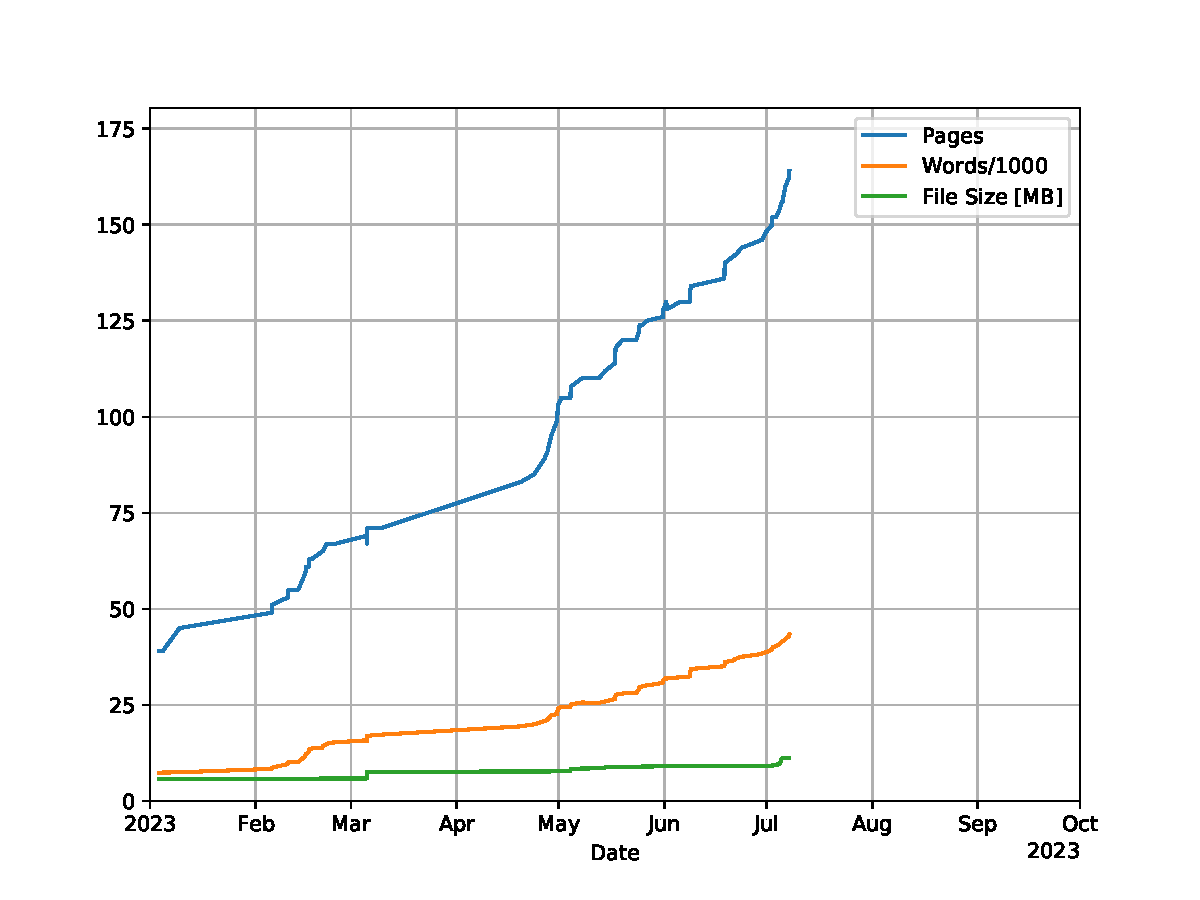
\includegraphics[width=\textwidth]{Figs/pdfstats_plot.pdf}
    \caption[]
    {Plot showing the development of this thesis, as a function of time.}
\end{figure}
\end{dedication}


% ************************** Thesis Acknowledgements **************************

\begin{acknowledgements}      

\textit{No man is an island, entire of itself; every man is a piece of the continent, a part of the main}\footnote{\textit{John Donne, Devotions upon Emergent Occasions}}. 
This is especially true in Experimental Particle Physics, which in recent decades has required large collaborations of people working together to explore the new frontiers. The making of this thesis is no different; I am deeply indebted to a great number of people who have helped me along the way. Here are some small words of thanks to you all.

To Armin Reichold, thank you so much for being my supervisor: always being there to ask the right questions about my work, and giving me advice about what to look at next. I made it through fighting SMELLIE thanks to your help. I've had so much fun doing research with you, learning so much thanks in part to your words to me: ``No black boxes''.

To Steve Biller and Jeff Tseng, your advice on matters of analysis, statistics, and computing have been invaluable. My work would be a shambles otherwise. Thank you also for building such a welcoming place to do Physics.

To Kim Proudfoot and Sue Geddes, who are the primary reason why the Particle Physics sub-department runs in any capacity. Also, to the IT Support staff; my work literally could not have been done without you guys keeping the interactive machines and internet connections working nicely. I'm sorry, Vip, for blocking the queue that time.

To the ever-growing family of colleagues and friends who I have had the pleasure of working in the SNO+ office with: Tereza, Iwan, Josh, Rafael, Cal, Gulliver, Abi, Jasmine, Qingyang, and Ellie. Special thanks to Josie for being an awesome thesis-writing buddy, and a brilliant friend. Also, to the elite strike squad of postdocs: Ed, Will, Ana Sofia, and Ben. I would be remiss in forgetting all the folks who have worked on SMELLIE, including Esther Turner and Jeff Lidgard. Jeff, thanks so much for being willing to fight through SMELLIE `integration hell' with me.

To Vic, Sierra, Caroline, Steph, Cindy, Matt, Mark, Aleksandra, Christine, and Ryan, thanks so much for making Sudbury so inviting whilst I was there; be it stuck underground without power, singing at Little Montreal, sliding on inflatables on Ramsey Lake, or getting stuck in Espanola. James and Rafael (again), it was great fun being housemates. Juliette, thanks for being my partner-in-crime as YM representatives: I hope your canoe is still okay.

To my friends outside the SNO+ cult, you are what makes life worth living: Eimear, Soniya, Ynyr, Ciaran, Niamh, Steph, Gwen, Sol, Ben, and so many others. Also, to everyone I've played with in Quadball (n\'{e}e Quidditch). Never Forget to be Awesome.

And finally, to my family: Mum, Dad, Joel, Ben, Leo, and Crumble. Thank you all for being so loving and fun, even after so many months in lockdown together. I would not be here without you. \textit{...All shall be well, and all shall be well, and all manner of thing shall be well.}\footnote{\textit{Julian of Norwich}}

\end{acknowledgements}

% ************************** Thesis Abstract *****************************
% Use `abstract' as an option in the document class to print only the titlepage and the abstract.
\begin{abstract}
This is where you write your abstract ...
\end{abstract}

\chapter*{Statement of Authorship}
The nature of contemporary experimental particle physics is that the research work is highly collaborative. The SNO+ experiment, which this thesis is about, is an 80+ member Collaboration and as such is no exception. As a result, the work discussed in this thesis is in many places built upon the tireless work of many others within the Collaboration. This Statement, as well as throughout the thesis itself, endeavours to note where the author himself did the research, and where work was taken from others.

Chapters~\ref{chap:theory} and \ref{chap:detector} cover the background knowledge of neutrino physics as well as the SNO+ detector needed to best understand the work performed in the rest of this thesis. This information has been compiled from a variety of books, journal articles, theses, and SNO+ internal technical reports. The author was trained as both a detector `operator' and `expert', taking dozens of shifts to monitor the detector whilst it was taking data, as well as being on-call to help if any issues arose with the detector electronics. The author also made numerous contributions to the Collaboration's central software package, \texttt{RAT}.

Chapters~\ref{chap:smellie_hardware}--\ref{chap:smellie_analysis} cover the work done by the author on the SMELLIE optical calibration system for SNO+. This calibration system historically been built and analysed by multiple people, including: Krishanu Majumdar, Esther Turner, Stephanie Langrock, and Jeff Lidgard. The author installed multiple pieces of new hardware for SMELLIE on-site, with help from Armin Reichold and Jeff Lidgard. With the same team, the author also helped to integrate the new hardware with the existing SMELLIE server software so that the newly-installed hardware could actually be effectively used. The author has taken dozens of hours of calibration data using SMELLIE throughout the course of the DPhil, both by himself and alongside Armin Reichold, Jeff Lidgard, and Ana Sofia In\'{a}cio.

Chapter~\ref{chap:beam_profiling} considers improvements to the simulation of SMELLIE events; the work done by Esther Turner on this subject is considered as a starting point. The rest of the chapter covers a new simulation approach created and developed by the author. Similarly, the scattering analysis performed within Chapter~\ref{chap:smellie_analysis} was inspired from the analyses done by Krishanu Majumdar, Esther Turner, and Stephanie Langrock. However, the work in this thesis uses a new method created by the author, and uses new scintillator phase data taken by the author. Also in this chapter is a separate analysis of this same data to measure the scintillator's extinction length. This was a novel analysis for SMELLIE, designed and implemented entirely by the author.

Finally, Chapter~\ref{chap:solar_osc_analysis} describes an analysis of scintillator phase data performed by the author to measure the solar neutrino oscillation parameters. An initial background-free sensitivity study of this topic was originally performed by Javier Caravaca. However, the work done by the author in this thesis analyses actual data, includes all relevant backgrounds appropriately, and considers systematics. Projections of expected sensitivity with greater livetime were also performed by the author. The analysis made by the author also uses a Bayesian MCMC approach, using the \texttt{OXO} signal extraction software framework initially built by Jack Dunger. A number of further people have since improved \texttt{OXO}, including the author: substantial improvements to the handling of systematics floated within the MCMC fit, as well as allowing for the floating of oscillation parameters within the fit.

% *********************** Adding TOC and List of Figures ***********************

\tableofcontents

\listoffigures

\listoftables

% \printnomenclature[space] space can be set as 2em between symbol and description
%\printnomenclature[3em]

\printnomenclature

% ******************************** Main Matter *********************************
\mainmatter

\addcontentsline{toc}{chapter}{Introduction}
\chapter*{Introduction}\label{chap:intro}
{\color{blue} Couple of pages outlining document's structure and contents (this is what each of the chapters is here for). Less formal than the abstract, also explaining what the expected audience of this thesis is: who will find this document useful!}
%!TEX root = ../thesis.tex
%*******************************************************************************
%*********************************** First Chapter *****************************
%*******************************************************************************

\chapter{The Theory of Neutrino Physics}\label{chap:theory}
\setlength{\epigraphwidth}{.45\textwidth}
\epigraph{\textit{Light\\Light\\The visible reminder of Invisible Light}}{\textit{The Rock}\\\textsc{T. S. Eliot}}
\setlength{\epigraphwidth}{.4\textwidth}

\section{The Standard Model and Neutrinos}
% \subsection{A Brief Introduction to the Standard Model}
% Covering how the SM works at the highest level, including:
% \begin{itemize}
%     \item Quantum Field Theory and the Lagrangian dynamical framework
%     \item The connection between symmetries of a QFT model and its gauge fields that describe the model's forces
%     \item The SM's fundamental symmetries, and associated forces, but ---
%     \item Not (exactly) what we see ``normally''! The electromagnetic and weak forces appear distinct, and the weak gauge bosons have mass. To explain this, we need a further component, the Brout-Englert-Higgs (BEH) Mechanism. 
% \end{itemize}
% [2 pages total]
% \subsection{Neutrinos within the Standard Model}
\nomenclature{\textbf{SM}}{The Standard Model of Particle Physics}
The \textit{Standard Model} (SM) of Particle Physics is the culmination of a century's work by scientists to understand the fundamental constituent elements of the Universe, and their interactions. Within the SM, fundamental particles are excitations of associated quantum fields within spacetime. One class of particles in the SM are known as the neutrinos, $\nu$: these are spin-$1/2$ fermions which are neutral in both the strong and electromagnetic force. The only means by which they are known to interact is through the weak nuclear force. There are three `flavours' of neutrino, one associated with each of their charged lepton counterparts: the electron neutrino $\nu_e$, the muon neutrino $\nu_\mu$, and the tau neutrino $\nu_\tau$.

\nomenclature{\textbf{EW}}{Electroweak (Theory)}
Crucial to understanding the nature of neutrinos is their interactions with other particles. Within the SM, the weak nuclear force and electromagnetism are unified into the Electroweak (EW) Theory by the work of Glashow, Salam, and Weinberg~\cite{glashowPartialsymmetriesWeakInteractions1961,weinbergModelLeptons1967,salamWeakElectromagneticInteractions1994}. % Cite foundational EW papers
This is a so-called \textit{chiral gauge field theory}. Gauge field theories are a special type of quantum field theory which demand that the Lagrangian density $\mathcal{L}$ is invariant under certain kinds of transformation, in addition to the usual requirement of Lorentz invariance. For EW, the Lagrangian is invariant under `local' transformations of the fields' internal degrees of freedom, defined by the `gauge' group $SU(2)_{L}\times U(1)_{Y}$, where $L$ and $Y$ are known as the left-handed weak isospin and weak hypercharge, respectively.

A local transformation is one which changes values of the fields at all points in spacetime. By demanding invariance under these gauge transformations, as well as Lorentz invariance, the theory naturally predicts the existence of vector (spin-1) boson particles. These are known as the `gauge' bosons of the theory, and they mediate the interactions defined by the gauge group. The massive $W^{\pm}$ and $Z^{0}$ bosons, discovered by the UA1 and UA2 experiments in 1983~\cite{arnisonExperimentalObservationIsolated1983,bannerObservationSingleIsolated1983,arnisonExperimentalObservationLepton1983}, % CITE!!!
mediate the weak nuclear force, whilst the massless photon $\gamma$ mediates the electromagnetic force.

The theory of EW interactions is also \textit{chiral}. Any spinor that defines the wavefunction of a spin-$1/2$ field can be split into its left- and right-handed `chiral' components, defined through the projection operators $P_{L,R} = \frac{1\mp\gamma^{5}}{2}$. The force associated with the $SU(2)_{L}$ part of the EW gauge group only interacts with the left-handed components of particles, denoted with the subscript $L$ on their wavefunction.

\nomenclature{\textbf{NC}}{Neutral Current (weak interaction)}
\nomenclature{\textbf{CC}}{Charged Current (weak interaction)}
The Lagrangian that defines the weak interactions of neutrinos is:
\begin{equation}
    -\mathcal{L} = \frac{g}{2\cos{\theta_{W}}}\sum_{\ell,L}\bar{\nu}_{\ell,L}\gamma^{\mu}\nu_{\ell,L}Z^{0}_{\mu}
    +\frac{g}{\sqrt{2}}\sum_{\ell}\bar{\nu}_{\ell,L}\gamma^{\mu}\ell^{-}_{L}W^{+}_{\mu} + \mathrm{h.c.}.
\end{equation}
Here, $g$ is the dimensionless coupling constant associated with $SU(2)_{L}$, and $\theta_{W}$ is the Weinberg angle. The three lepton flavour fields are denoted by $\ell=e,\mu,\tau$, with their associated neutrino fields being given by $\nu_{\ell}$. Similarly, the fields associated with the weak gauge bosons are given by $W^{\pm}$ and $Z^{0}$. The two components of this Lagrangian are known as the Neutral Current (NC) and Charged Current (CC) weak interactions of neutrinos, respectively. Similar Lagrangians exist that define the NC and CC interactions of quarks, as well as the NC interactions of the charged leptons.

\nomenclature{\textbf{IBD}}{Inverse $\beta$-decay}
Solidifying this theoretical picture are decades-worth of experimental tests of neutrinos and their place in the SM. The first neutrinos to be detected were electron anti-neutrinos, by Cowan and Reines in 1956~\cite{cowanDetectionFreeNeutrino1956,reinesNeutrino1956}. % cite Reines and Cowen.
These neutrinos were generated in the $\beta$-decay of radioactive isotopes within the Savannah River nuclear reactor: \ce{n \to p + e^{-} + \bar{\nu}_{e}}. This decay arises from a down quark within the neutron of an atom converting into an up quark via a CC interaction, generating a virtual $W^{-}$ boson that promptly decays into an electron and $\bar{\nu}_{e}$. The method by which Cowen and Reines detected these anti-neutrinos was through \textit{inverse $\beta$-decay} (IBD): \ce{\bar{\nu}_{e} + p \to e^{+} + n}. This process also originates from CC interactions. Analogous CC interactions allowed Danby \textit{et al} to discover the muon neutrino in 1962~\cite{danbyObservationHighEnergyNeutrino1962}, % cite Lederman, Schwarts, Steinberger
and the DONUT Collaboration to discover the tau neutrino in 2000~\cite{kodamaObservationTauNeutrino2001}. % cite DONUT Collaboration

The existence of NC interactions with neutrinos and anti-neutrinos was first demonstrated by the Gargamelle experiment in 1974~\cite{hasertObservationNeutrinolikeInteractions1973,hasertSearchElasticMuonneutrino1973,hasertObservationNeutrinolikeInteractions1974,blietschauEvidenceLeptonicNeutral1976}. % cite gargamelle
In particular, the observation of anti-muon neutrino electron elastic scattering, \ce{\bar{\nu}_{\mu} + e^{-} \to \bar{\nu}_{\mu} + e^{-}} by the experiment was an unambiguous demonstration of NC interactions.

In 1958, Goldhaber \textit{et al}~\cite{goldhaberHelicityNeutrinos1958} were able to demonstrate experimentally that the helicity of electron neutrinos, i.e. the component of their spin along the direction of motion, is $-1$. No evidence of neutrinos with positive helicities (or equally, anti-neutrinos with negative helicities) exists. This stands in firm contrast to all other SM particles.

No flavours of neutrino beyond the electron, muon, or tau types have been discovered. A combined analysis of data from the four LEP experiments looking at the decay width of the $Z$ boson was able to indirectly measure the number of neutrino species that could undergo NC interactions and had masses less than one half of the $Z$ boson: $N_{\nu} = 2.9963\pm0.0074$~\cite{PrecisionElectroweakMeasurements2006,janotImprovedBhabhaCross2020}. % cite LEP papers, including update with correction!
This measurement is very strong evidence that no other `light' weakly-interacting neutrinos exist.


% \begin{itemize}
%     \item Basic description of where neutrinos fit into SM: 3 kinds of neutral fermion, the counterparts to the charged fermions. Interacts with the weak force only.
%     \item Summary of the experimental evidence for this picture: mainly, the discovery of electron anti-neutrinos by Cowan and Reines, the muon neutrino by Lederman, Schwartz, and Steinberger, and the tau neutrino by the DONUT Collaboration. Further critical experiments include the first measurement of a neutrino's helicity by Goldhaber et al. as well as Danby et al.'s demonstration that $\nu_{\mu}$ are distinct from $\nu_{e}$.
%     \item More detailed description, via Feynman diagrams, of the two fundamental modes of interaction by neutrinos with the weak force: charged- and neutral-current interactions. A brief mention of the quantitative theory that underlies description: Gashow, Salam, and Weinberg's Electroweak Theory. This explains not only the V--A structure of charged-current interactions, but also predicted accurately the nature of neutral-current interactions. (Given space constraints, I see no reason to go into much of the details of the theory, or the many experimental tests of its structure.)
% \end{itemize}

% [4 pages]
\section{Neutrino Oscillations and Neutrino Masses}
So far in this description, no attempt has been made to explain the origin of the masses of the fundamental particles. It is certainly straightforward to na\"{i}vely add a mass term such as $m_{e}\bar{e}_{L}e_{R}$ into the SM Lagrangian, where $m_e$ is the mass of the electron. However, one can show that any mass terms added will necessarily violate the $SU(2)_{L}\times U(1)_{Y}$ symmetry that defines the EW interactions~\cite{deppischChapterNeutrinosStandard2019}. % should cite something appropriate.
The weak vector bosons $W^{\pm}$ and $Z$ would then need to be massless, in contradiction with observations.

\nomenclature{\textbf{BEH}}{Brout-Englert-Higgs (Mechanism)}
The solution to this problem comes in the form of the \textit{Brout-Englert-Higgs (BEH) Mechanism}~\cite{englertBrokenSymmetryMass1964,higgsBrokenSymmetriesMasses1964,guralnikGlobalConservationLaws1964}, % cite BEH theory papers
the final component of the SM.  In this Mechanism, an additional two-component ``Higgs'' field $H$ is proposed, which is able to interact with the other fields of the theory in a manner that preserves the SM gauge symmetries. One part of the added Higgs field interactions are the so-called Yukawa terms, which for interactions with leptons are given by:
\begin{equation}\label{eq:SM_yukawa_leptons}
    -\mathcal{L}_{\mathrm{Yukawa,lep}} = \sum_{\ell}y_{\ell}\bar{L}^{\ell}H\ell^{c} + \mathrm{h.c.},
\end{equation}
where $y_{\ell}$ are the ``Yukawa'' coupling constants for the three lepton flavours, $L^{\ell} = \begin{pmatrix}
    \nu_{\ell,L} \\ \ell_{L}
\end{pmatrix}$ are the left-handed lepton doublets of the SM, and $\ell^{c}$ are the right-handed charged leptons.

\nomenclature{\textbf{SSB}}{Spontaneous Symmetry Breaking}
The key to the BEH Mechanism is \textit{Spontaneous Symmetry Breaking} (SSB): the Higgs field is defined in such a way that the ground state takes a non-zero `vacuum expectation value', $v$. By doing so, the underlying gauge symmetry of the EW interactions is spontaneously broken as $SU(2)_{L}\times~U(1)_{Y}\to~U(1)_{Q}$, where $U(1)_{Q}$ is the residual electromagnetic charge conservation. The above Yukawa Lagrangian term after symmetry breaking generates the mass terms for the charged leptons:
\begin{equation}
    -\mathcal{L}_{\mathrm{Yukawa,lep}} \to \sum_{\ell}m_{\ell}\bar{\ell}_{L}\ell^{c} + \mathrm{h.c.},
\end{equation}
where $m_{\ell} = \frac{v}{\sqrt{2}}y_{\ell}$ are the charged lepton masses. Other terms associated with Higgs interactions in the SM generate mass terms for the quarks and weak vector bosons, as seen in data. A further prediction of this BEH Mechanism is the existence of a massive scalar boson known as the Higgs particle; this was discovered in 2012 by the ATLAS and CMS Collaborations~\cite{aadObservationNewParticle2012,chatrchyanObservationNewBoson2012}. %cite Higgs discovery papers

The one type of fundamental particle not covered by the above argument are neutrinos. If neutrinos were massless, then there is no issue: we observe neutrinos to have only negative helicities, which is equal to left-handed chiralities if they are massless. As the SM contains no right-handed neutrinos, no Yukawa interaction can be built to generate masses for the neutrinos. One can also demonstrate that, in the SM, neutrinos cannot even obtain masses through loop corrections~\cite{workmanReviewParticlePhysics2022}. % cite PDG review 14

This assumption of massless neutrinos appears initially consistent with the current observations of direct neutrino mass measurements. The strongest direct limits come from the KATRIN experiment, which looks at the endpoint of the tritium $\beta$-decay spectrum. The `effective'\footnote{
    KATRIN measures the `effective' mass and not the actual mass, because of the phenomenon of neutrino oscillations as described in the following sections.
} electron anti-neutrino mass was measured to be $m_{\nu} < \SI{0.8}{\eV}$ at a 90\% confidence level~\cite{akerDirectNeutrinomassMeasurement2022}. % cite https://inspirehep.net/literature/1863711
Even stronger limits are available from cosmology, by looking in part at the power spectrum of the Cosmic Microwave Background. Assuming the so-called Standard `$\Lambda$CDM' Model of Cosmology, limits on the sum of all three neutrino flavours $\sum m_{\nu}<\mathcal{O}(\SI{0.1}{\eV})$ have been achieved~\cite{divalentinoMostConstrainingCosmological2021}. % cite a couple of papers, maybe.

\subsection{The Evidence for Neutrino Oscillations}\label{sec:nu_osc_evidence}
Despite the current lack of any direct measurements, we now know that at least some neutrino flavours must have mass. This is because of the phenomenon of \textit{neutrino oscillations}, which have been observed over a variety of experiments and contexts. The critical pieces of evidence for this process are described here; the underlying mathematical model that is used to explain them quantitatively is described in Section~\ref{sec:nu_osc_phenom}.

\subsubsection{The Solar Neutrino Problem}
\nomenclature{\textbf{SSM}}{Standard Solar Model}
Neutrinos are generated from the Sun as a by-product of the fusion reactions at its core. At the highest level, protons fuse into alpha particles by the overall reaction \ce{4p \to ^{4}He{} + 2e^{+} + 2\nu_{e}}, generating also $\sim\SI{25}{\MeV}$ of energy that enables the Sun to shine~\cite{bahcallNeutrinoAstrophysics1989}. % cite Bahcall Neutrino Astrophysics.
This process is known as `hydrogen burning'. The Standard Solar Model (SSM) is the current best quantitative description of stellar evolution for main sequence stars, and our Sun in particular. It covers the nuclear reactions that generate both the energy that powers the star and the changes in the relative isotopic abundances, how the energy is transported out through the star via radiation of photons and convection, and how the outward pressures caused by this radiation is balanced by gravity to maintain hydrostatic equilibrium. An introduction to the SSM can be found in~\cite{bahcallNeutrinoAstrophysics1989}. % cite Bahcall's book again.

In the Sun, two sets of nuclear reactions enable hydrogen burning to occur: the \textit{proton-proton (pp) chain} and \textit{CNO cycle}. Diagrams of these reaction chains are shown in Fig.~\ref{fig:solar_nu_chains}. In the pp chain, protons are first fused together to form a \ce{^{2}H} nucleus through the `pp' and `pep' reactions, the latter also using an electron. Both of these processes are weak interactions that generate an electron neutrino. Once a deuterium nucleus has been generated, it strongly interacts with a proton to create a \ce{^{3}He} nucleus. The dominant method for hydrogen burning to then terminate is for two \ce{^{3}He} nuclei strongly interact to generate \ce{^{4}He} and two protons.

\begin{figure}
    \centering
    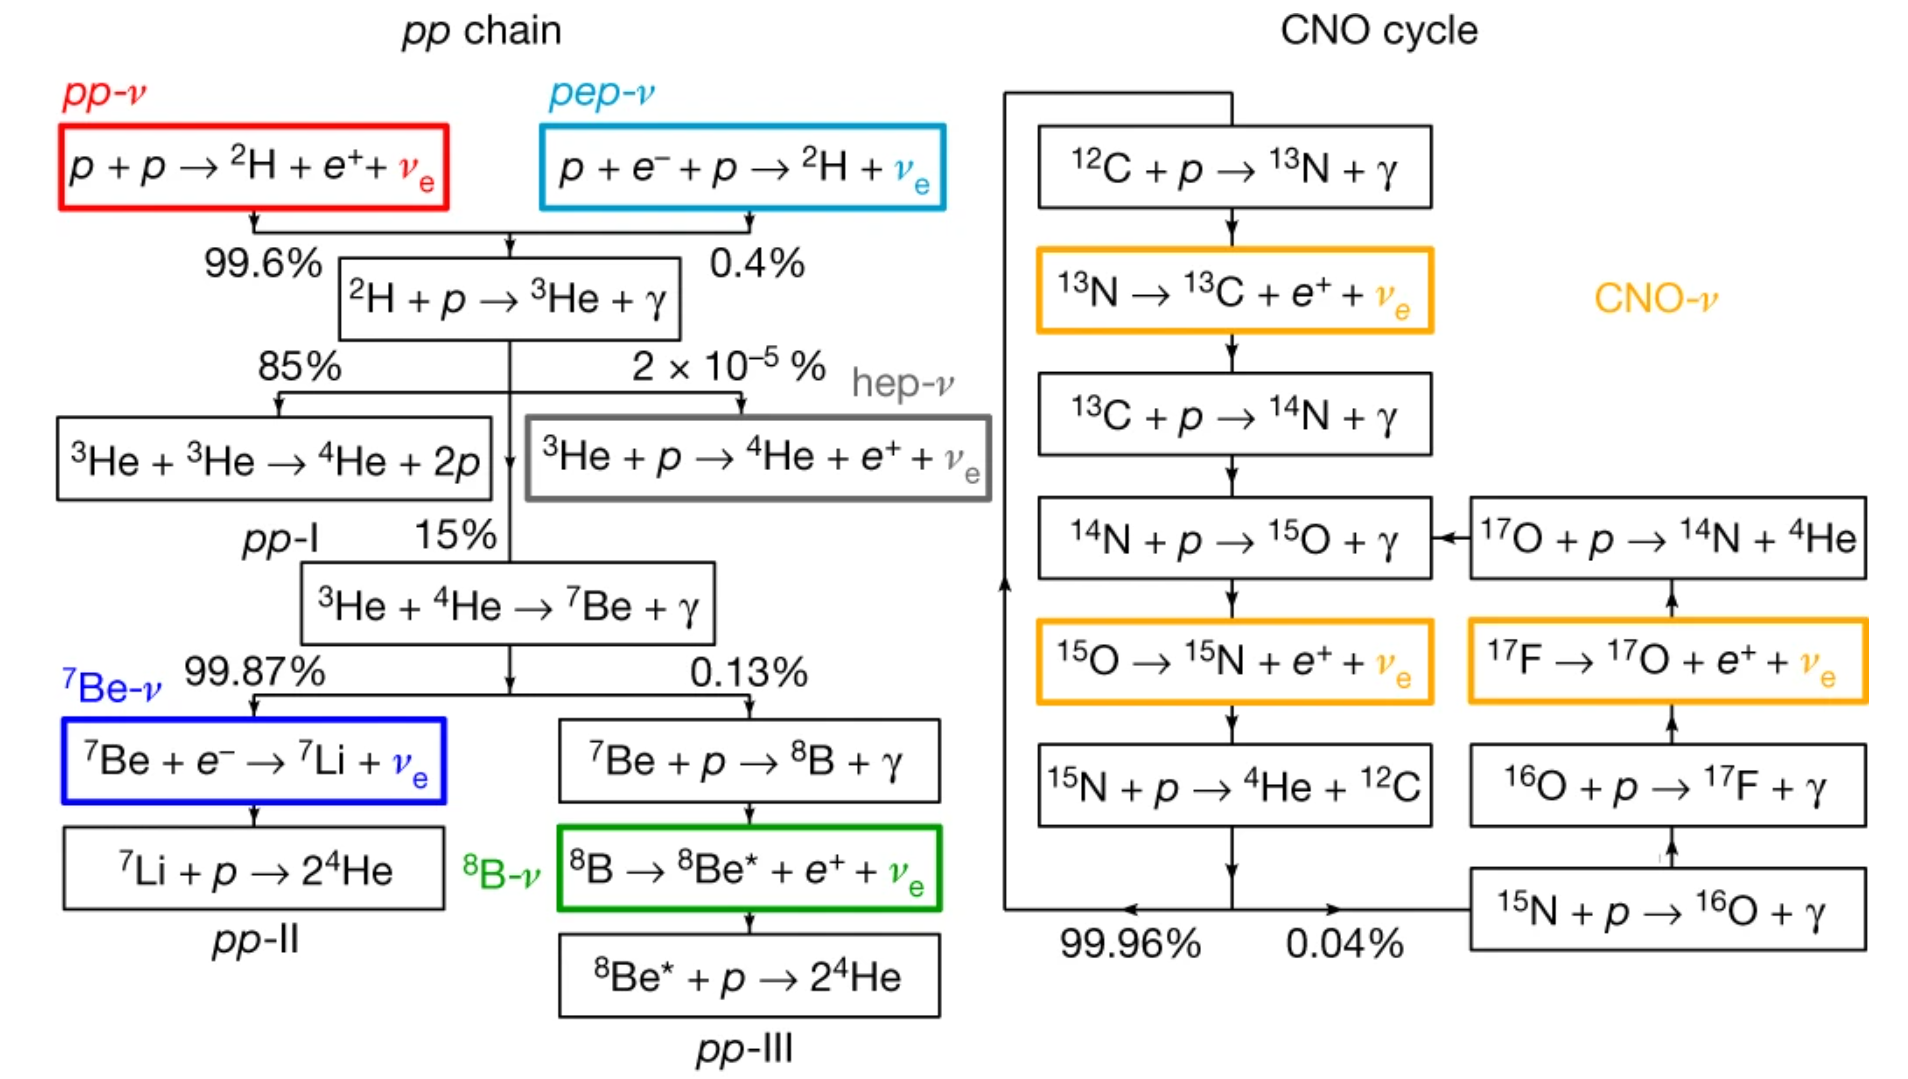
\includegraphics[width=\textwidth]{1_NeutrinoTheory/Figs/solar_nu_chains_diagram.png}
    \caption[Diagram of the pp chain and CNO cycle within the Sun]
    {Diagram of the pp chain and CNO cycle within the Sun, with the reactions that generate neutrinos highlighted. Taken from~\cite{agostiniComprehensiveMeasurementPpchain2018}.}
    \label{fig:solar_nu_chains}
\end{figure}

Two other nuclear reactions with \ce{^{3}He} are possible. In one, \ce{^{3}He} fuses with \ce{^{4}He} to generate a \ce{^{7}Be} nucleus, which can then generate a neutrino either from the creation of \ce{^{7}Li} via electron capture, or from the additional fusing into \beight{} which promptly $\beta^{+}$-decays. These are known as the \ce{^{7}Be} and \beight{} solar neutrino generation reactions, respectively. The final and rarest reaction within the pp chain that generates a neutrino is the so-called `hep' reaction, in which \ce{^{3}He} directly fuses with a proton.

The CNO cycle is a secondary means by which the Sun can burn hydrogen. This is achieved through the aid of a \ce{^{12}C} nucleus as a catalyst. Part of the cycle involves the generation of unstable isotopes \ce{^{13}N} and \ce{^{15}O}, both of which \ce{\beta^{+}}-decay, creating electron neutrinos. In a rare side-chain of the CNO cycle, it is possible to also generate \ce{^{17}F} which also weakly decays to generate a neutrino. This is the final method of generating neutrinos in our Sun.

The SSM quantitatively predicts the flux and energy spectra of neutrinos generated through each of the above processes, as incident on the Earth. This is shown in Fig.~\ref{fig:ssm_neutrino_spectra}. The shapes of the energy spectra are determined by the nuclear reactions that define the process: for example, the broad shape of the \beight{} $\nu_{e}$ energy spectrum comes from the $\beta^{+}$-decay of \beight{} isotopes, and has been measured in nuclear beam experiments to high precision~\cite{winterB8NeutrinoSpectrum2006}. % citation of B8 shape measurement by Winter et al.

\begin{figure}
    \centering
    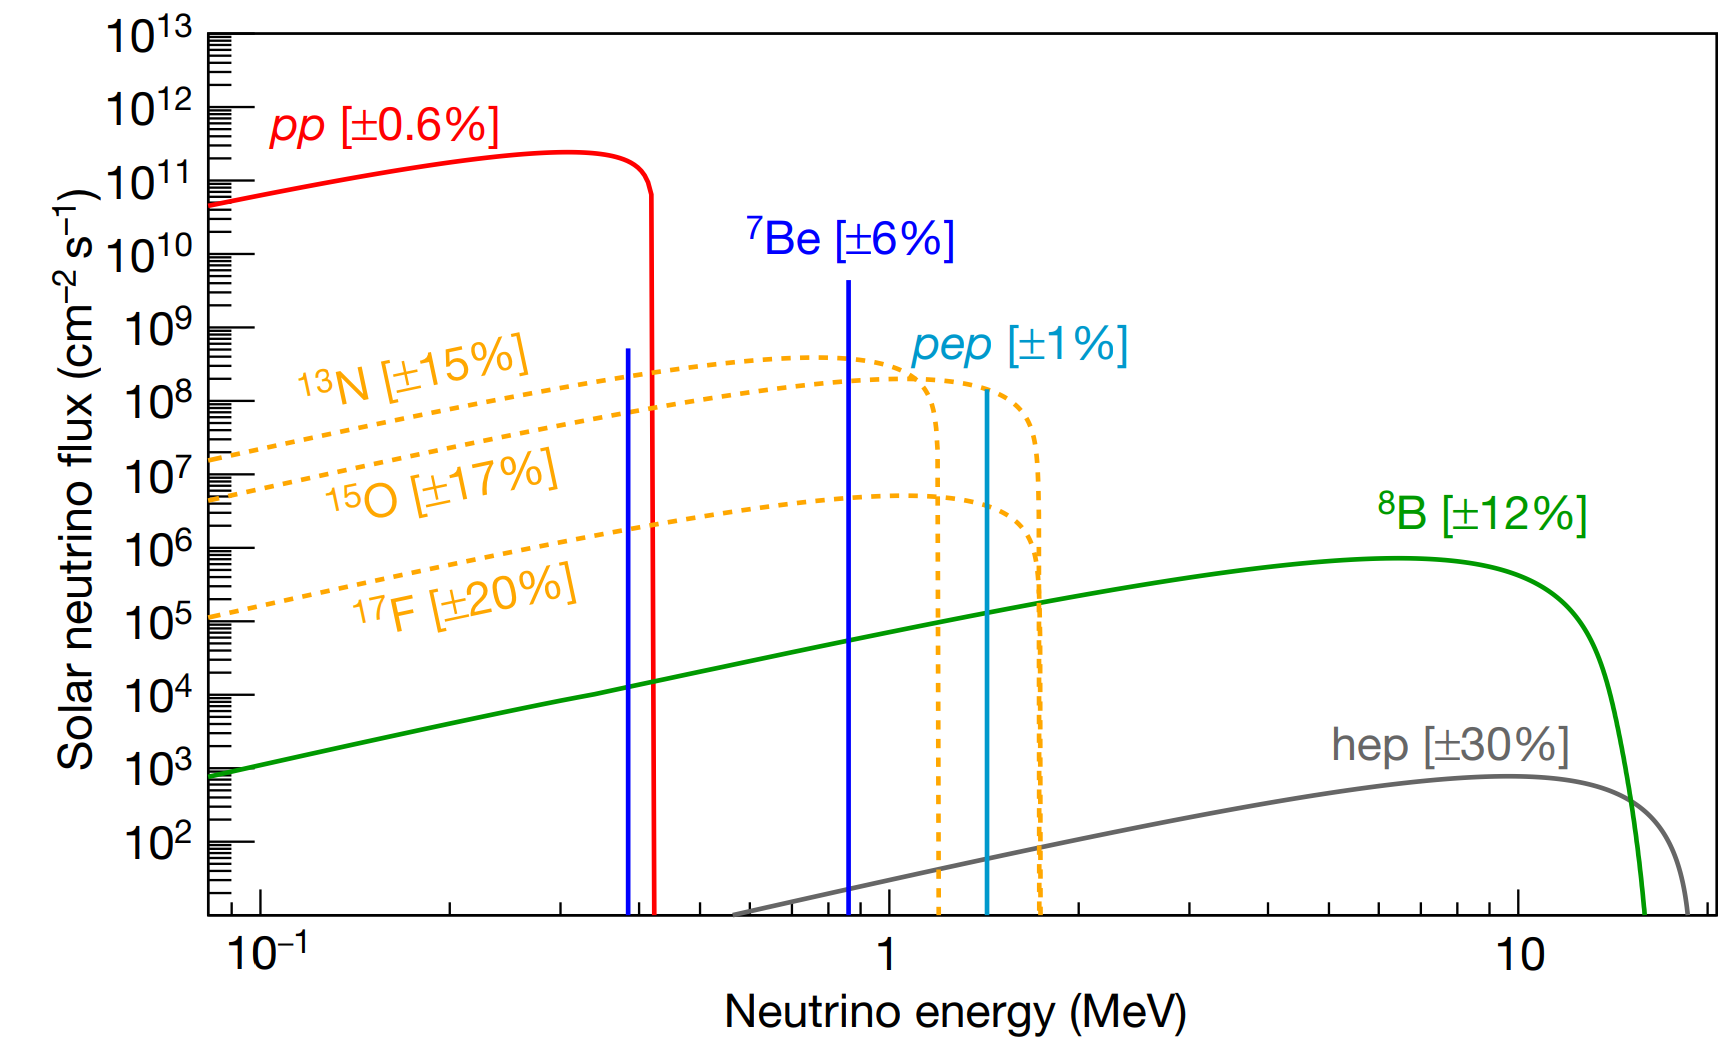
\includegraphics[width=0.8\textwidth]{1_NeutrinoTheory/Figs/solar_nu_energy_spec_SSM.png}
    \caption[Solar neutrino energy spectrum, and associated uncertainties from the SMM]
    {Solar neutrino energy spectra, and associated uncertainties from the SSM. Figure is taken from~\cite{agostiniComprehensiveMeasurementPpchain2018,vinyolesB16StandardSolar2018}; note that the flux is given in units of \si{\per\cm\squared\per\second\per\MeV} for the continuum sources, and \si{\per\cm\squared\per\second} for mono-energetic sources.}
    \label{fig:ssm_neutrino_spectra}
\end{figure}

The rate of the \beight{} interaction in the Sun, and hence the generated neutrino flux, depend strongly on the radial temperature distribution of the Sun, the cross-sections of the pp chain nuclear reactions, and the Sun's chemical composition. The latter point remains a topic of some controversy: measurements of the relative abundances in 1998 through spectroscopy of the Sun's photosphere as well as meteorites give a `metal-to-hydrogen' ratio of $Z/X = 0.023$~\cite{grevesseStandardSolarComposition1998}, whereas a more recent study in 2009 has a substantially lower value of $Z/X = 0.018$~\cite{asplundChemicalCompositionSun2009}. `Metal' here is used in the astrophysical sense: elements heavier than hydrogen or helium. These two models are called the `high-metallicity' \texttt{GS98} model and `low-metallicity' \texttt{AGSS09met} model, respectively. The current best SSM associated with these two abundance models, denoted \texttt{B16\_GS98} and \texttt{B16\_AGSS09met}, have \beight{} flux predictions of $\Phi_{\beight{}} = (5.46\pm12\%)\times 10^{6}\,\si{\per\cm\squared\per\second}$ and $\Phi_{\beight{}} = (4.50\pm12\%)\times 10^{6}\,\si{\per\cm\squared\per\second}$, respectively~\cite{vinyolesB16StandardSolar2018}.

\nomenclature{\textbf{SNU}}{Solar Neutrino Unit, defined as $10^{-36}$ neutrino interactions per second}
The first experiment built to measure solar neutrinos was that of the Homestake Chlorine Detector, starting in the late 1960s~\cite{davisSearchNeutrinosSun1968}. A large tank of \ce{C_{2}Cl_{4}} was put deep underground, whereby electron neutrinos could be captured by the \ce{^{37}Cl} nuclei: \ce{^{37}Cl{} + \nu_{e} \to ^{37}Ar{} + e^{-}}. Through a careful chemical extraction process, any atoms of \ce{^{37}Ar} generated in the tank could be counted with an efficiency over 90\%. After running the experiment for a period of almost 30 years, a final measurement of the solar neutrino interaction rate was $2.56\pm0.16(\mathrm{stat.})\pm0.16(\mathrm{sys.})\,\mathrm{ SNU}$~\cite{clevelandMeasurementSolarElectron1998}, % cite Ray davis
where 1 SNU (`Solar Neutrino Unit') is defined as $10^{-36}$ events per target atom per second. The results as a function of time can be seen in Fig.~\ref{fig:homestake_results}.

\begin{figure}
    \centering
    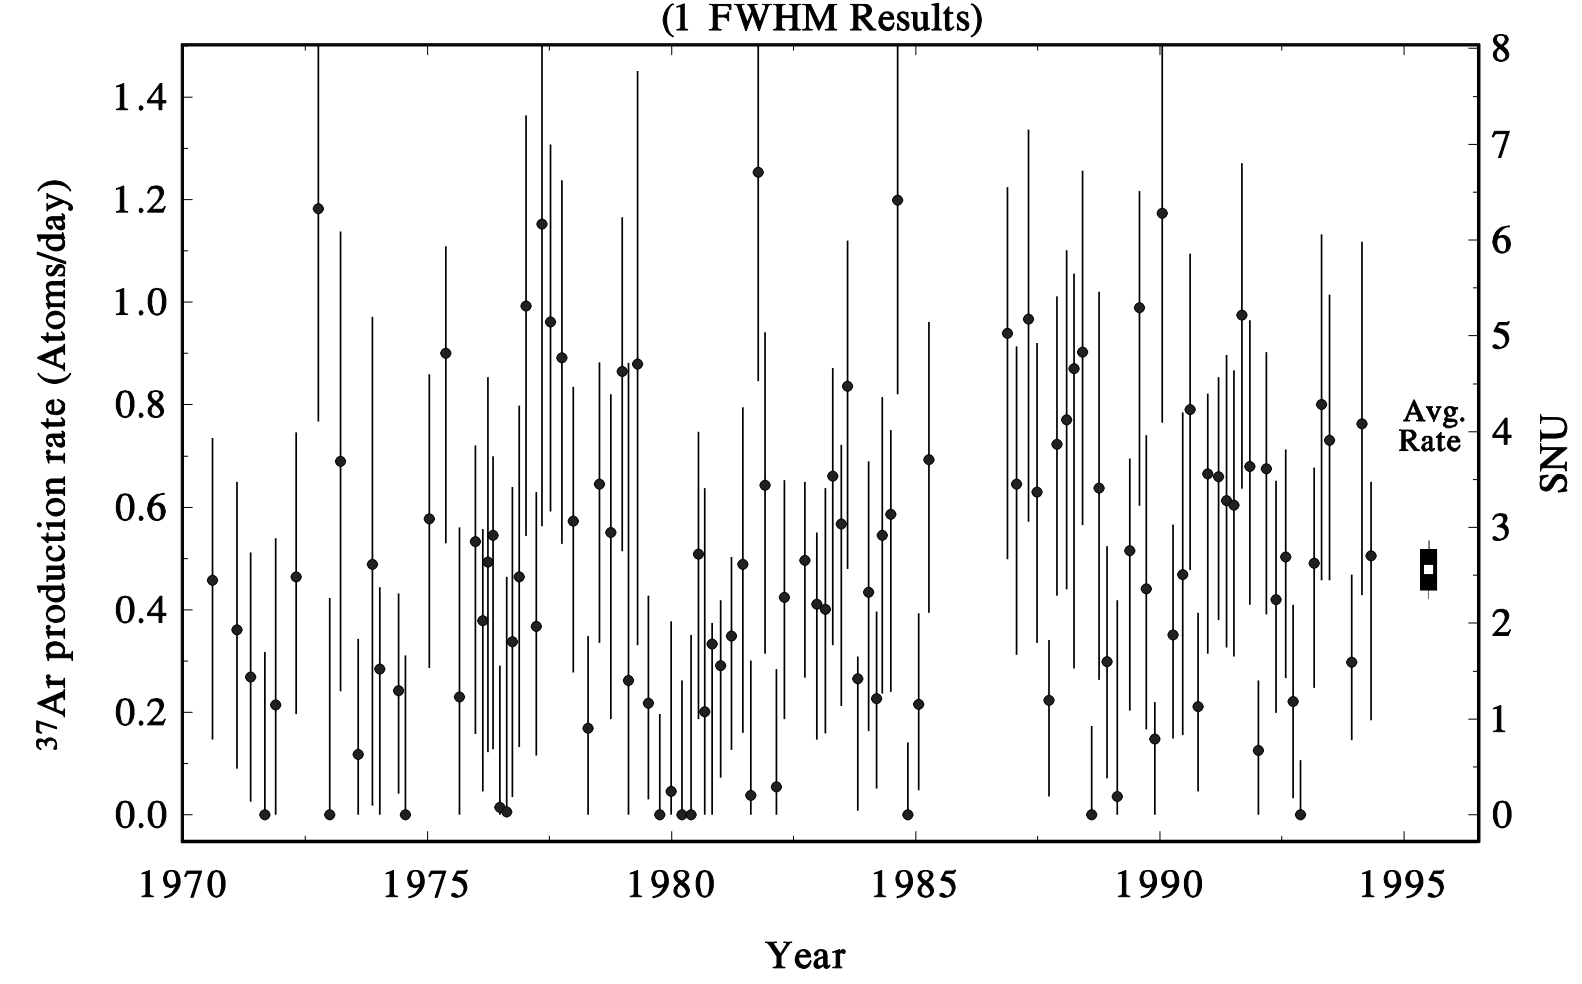
\includegraphics[width=0.8\textwidth]{1_NeutrinoTheory/Figs/homestake_summary_results.png}
    \caption[]{Observed rate in the Homestake Chlorine detector, over the lifetime of the experiment. Taken from~\cite{clevelandMeasurementSolarElectron1998}.}
    \label{fig:homestake_results}
\end{figure}

In contrast, according to one particular recent SSM using the GS98 metallicity model, the expected rate is $8.46^{+0.87}_{-0.88}\,\mathrm{ SNU}$~\cite{pena-garaySolarNeutrinosSolar2008}, highly inconsistent with the results at Homestake. This disagreement became known as the \textit{Solar Neutrino Problem}, and was the first piece of evidence towards neutrino oscillations.

Since the Homestake experiment, a series of solar neutrino experiments used a variety of different target isotopes to measure the rate of solar neutrinos. In all cases, the measured rates were substantially below what is expected from the SSM. The SAGE and GALLEX/GNO experiments used the capture of electron neutrinos on \ce{^{71}Ga} to measure the capture rate: the final observations were $65.4^{+3.1}_{-3.0}(\mathrm{stat.})\,^{+2.6}_{-2.8}(\mathrm{sys.})\,\mathrm{ SNU}$~\cite{abdurashitovMeasurementSolarNeutrino2009} and $69.3\pm4.1\pm3.6\,\mathrm{ SNU}$~\cite{altmannCompleteResultsFive2005}, respectively. An SSM expectation is $127.9^{+8.1}_{-8.2}$~\cite{pena-garaySolarNeutrinosSolar2008}. Because the capture on \ce{^{71}Ga} has a much lower energy threshold than \ce{^{37}Cl}, these experiments were able to show that the Solar Neutrino Problem was associated with the low-energy pp neutrinos as much as the higher energy \beight{} and \ce{^{7}Be} neutrinos.

\nomenclature{\textbf{ES}}{Elastic Scattering}
The Kamiokande experiment, and its successor Super-Kamiokande, are large water Cherenkov detectors, sensitive to neutrinos through neutrino-electron elastic scattering (ES): $\nu_{x} + e^{-}\to\nu_{x} + e^{-}$. All flavours of neutrino are capable of scattering through a NC process, but there is an additional CC mode for electron neutrinos, as shown in Fig.~\ref{fig:nu_e_es_feynman_diagrams}. The differential cross-section for this interaction as a function of the scattered electron's kinetic energy $T$ is given by~\cite{bahcallSolarNeutrinosRadiative1995}: % cite Bahcall
\begin{align}\label{eq:enu_es_xsec}
    \frac{d\sigma_{\nu_{i}}}{dT} &= \frac{2G_{F}^{2}m_{e}}{\pi}\left\{
        g_{L}^{2}(T)\left[
            1 + \frac{\alpha}{\pi}f_{-}(z)
        \right]
        + g_{R}^{2}(T)(1-z)^{2}\left[
            1 + \frac{\alpha}{\pi}f_{+}(z)
        \right]\right.\nonumber\\
        &\qquad \left. {}
        -g_{R}(T)g_{L}(T)\frac{m_{e}}{E_{\nu}}\left[
            1 + \frac{\alpha}{\pi}f_{+-}(z)
        \right]
    \right\},
\end{align}
where $i = e, \mu$\footnote{
    $\frac{d\sigma_{\nu_{\mu}}}{dT} = \frac{d\sigma_{\nu_{\tau}}}{dT}$ because both flavours of neutrino only undergo the NC interaction.
}, $G_{F}$ is the Fermi coupling constant, $m_{e}$ is the electron mass, $\alpha$ is the fine-structure constant, $E_{\nu}$ is the incident neutrino energy, and $z = T/E_{\nu}$. $g_{L,R}(T)$ are the left- and right-handed running chiral couplings, which have a $T$-dependence because of radiative corrections. Similarly, $f_{-}(z)$, $f_{+}(z)$, and $f_{+-}(z)$ are all QED radiative correction terms. 
% Fig.~\ref{fig:nu_e_es_xsec} shows this differential cross-section for both $\nu_{e}$ and $\nu_{\mu}$ scattering. As can be seen, the cross-section for $\nu_{e}$ is $\sim 6$ times that of $\nu_{\mu}$, because of the additional CC interaction mode.

\begin{figure}
    \centering
    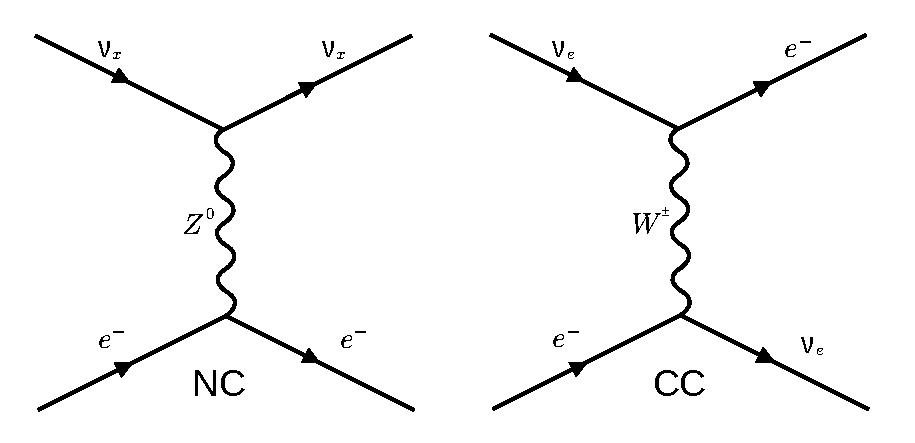
\includegraphics[width=\textwidth]{1_NeutrinoTheory/Figs/feynman_diag_nu_e_es.pdf}
    \caption[The two tree-level Feynman diagrams associated with neutrino-electron elastic scattering]
    {The tree-level Feynman diagrams associated with the NC and CC modes of neutrino-electron elastic scattering.}
    \label{fig:nu_e_es_feynman_diagrams}
\end{figure}

% \begin{figure}
%     \centering
%     % \includegraphics[]{}
%     \caption[]{}
%     \label{fig:nu_e_es_xsec}
% \end{figure}

The most recent combined measurement of the \beight{} solar neutrino flux in Super-Kamiokande is $(2.345\pm0.014(\mathrm{stat.})\pm0.036(\mathrm{sys.}))\times10^{6}\,\si{\per\cm\squared\per\second}$~\cite{abeSolarNeutrinoMeasurements2016}, roughly half the amount expected from the SSM~\cite{vinyolesB16StandardSolar2018}.

\nomenclature{\textbf{SNO}}{Sudbury Neutrino Observatory}
\nomenclature{\textbf{UPW}}{Ultra-pure water}
One of the most important experiments for demonstrating that neutrino oscillations are the solution to the Solar Neutrino Problem was the Sudbury Neutrino Observatory, SNO. A large spherical acrylic vessel \SI{2.2}{\km} underground was filled with \num{1000} tonnes of heavy water, \ce{D_{2}O}, from which Cherenkov light due to particle interactions could be detected~\cite{BOGER2000172}. Neutrinos were able to interact with the heavy water via three complementary modes: the CC process \ce{\nu_{e} + d \to e^{-} + 2p}, the NC process \ce{\nu_{x} + d \to \nu_{x} + p{} + n}, and the ES process described above.

Results of the measured fluxes of $\nu_{e}$ and $\nu_{\mu,\tau}$ solar neutrinos for the three detection modes in SNO, ES results from Super-Kamiokande, and comparison to the SSM are shown in Fig.~\ref{fig:sno_flux_results}. Because the NC interaction is insensitive to neutrino flavour, it is able to directly measure the total flux of \beight{} solar neutrinos, regardless of flavour. One can see that, from the results, the NC flux measurement is consistent with the SSM. In contrast, the CC mode is only sensitive to the $\nu_{e}$ flux, whilst the ES mode is sensitive to an admixture of the different neutrino flavours. The results of all measurements of solar neutrinos from both SNO and Super-Kamiokande lead to consistent values of the flux of \beight{} neutrinos for each flavour, consistent also with the SSM.

\begin{figure}
    \centering
    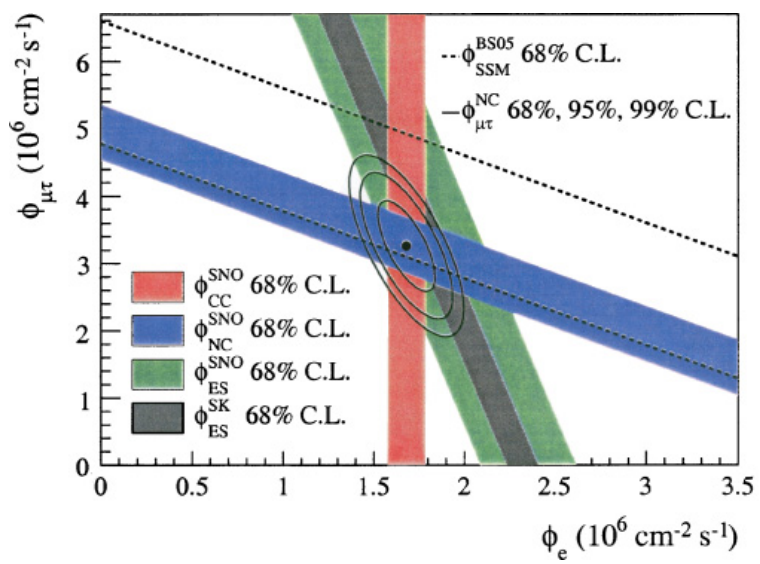
\includegraphics[width=0.7\textwidth]{1_NeutrinoTheory/Figs/sno_vs_ssm_comparison.png}
    \caption[Comparison of measured solar neutrino fluxes in the SNO CC, NC, and ES modes to the SSM]
    {Measured solar neutrino fluxes from electron neutrinos versus muon and tau neutrinos, in the SNO CC, NC, and ES modes (coloured bands). Also shown is the expectation from the SSM (dotted lines), and the ES rate measured from Super-Kamiokande (black band). The combined probability contours are shown in black. Taken from~\cite{aharmimElectronEnergySpectra2005}.}
    \label{fig:sno_flux_results}
\end{figure}

% ADD BOREXINO, KamLAND results???

\subsubsection{The Atmospheric Neutrino Anomaly}
Atmospheric neutrinos come from the decays of cosmic ray pions and muons in the Earth's atmosphere. One can show that the expected ratio of the flux of muon neutrinos to electron neutrinos generated in the atmosphere should be about 2~\cite{fukudaEvidenceOscillationAtmospheric1998}. % cite something!
The IBM~\cite{becker-szendyElectronMuonneutrinoContent1992}, % cite
Kamiokande~\cite{fukudaAtmosphericVmveRatio1994}, % cite
and Super-Kamiokande~\cite{fukudaEvidenceOscillationAtmospheric1998} % cite
experiments were able to detect atmospheric neutrinos through CC interactions with electrons in the water, generating electron or muon tracks (depending on the neutrino flavour) that could be distinguished by the shape of their Cherenkov rings. In all cases, the observed ratio of $\nu_{\mu}$ to $\nu_{e}$ events was consistently below expectations. This was known as the Atmospheric Neutrino Anomaly.

Super-Kamiokande was able to gather enough statistics from atmospheric neutrino interactions to demonstrate that there was a clear dependence on the rate of muon neutrino interactions as a function of the event direction. In particular, the asymmetry $A$ between the number of upward-going muon neutrino events $U$, and downward-going events $D$, was measured in one dataset to be~\cite{fukudaEvidenceOscillationAtmospheric1998}: % cite SK
\begin{equation*}
    A = \frac{U-D}{U+D} = -0.296 \pm 0.048(\mathrm{stat.}) \pm 0.01(\mathrm{sys.}),
\end{equation*}
a deviation from zero by over 6$\sigma$. In contrast, the asymmetry measured for atmospheric $\nu_{e}$ events was consistent with zero. Further analysis on the experiment looked at the rate of atmospheric $\nu_{\mu}$ events as a function of the ratio $L/E$, where $L$ is the estimated distance from production of the neutrino, and $E$ is the neutrino energy. The relative rate compared to expectations is shown in Fig.~\ref{fig:LE_plot_SK_atmos}. Taken together, these atmospheric neutrino results demonstrate that there is a disappearance of muon neutrinos which depends on the ratio $L/E$, whereas there is no similar effect for the electron neutrinos.

\begin{figure}
    \centering
    \begin{subfigure}{0.48\textwidth}
        \centering
        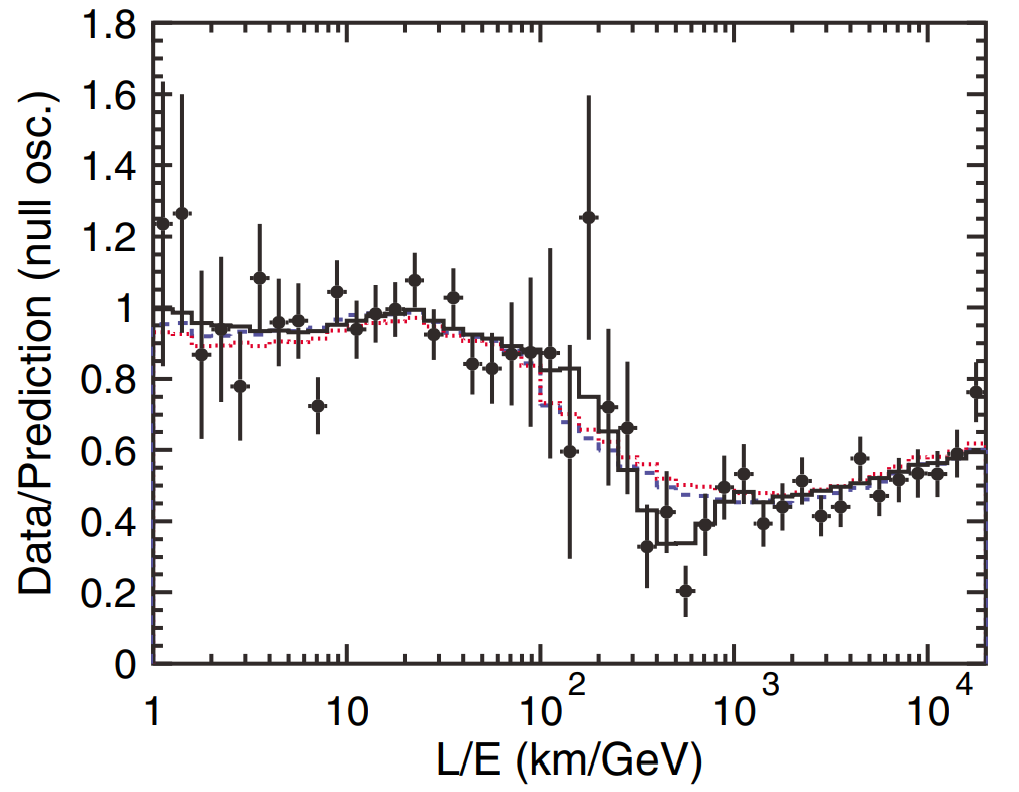
\includegraphics[width=0.95\linewidth]{1_NeutrinoTheory/Figs/sk_atmospherics_LE_plot.png}
        \caption{}
        \label{fig:LE_plot_SK_atmos}
    \end{subfigure}
    \begin{subfigure}{0.48\textwidth}
        \centering
        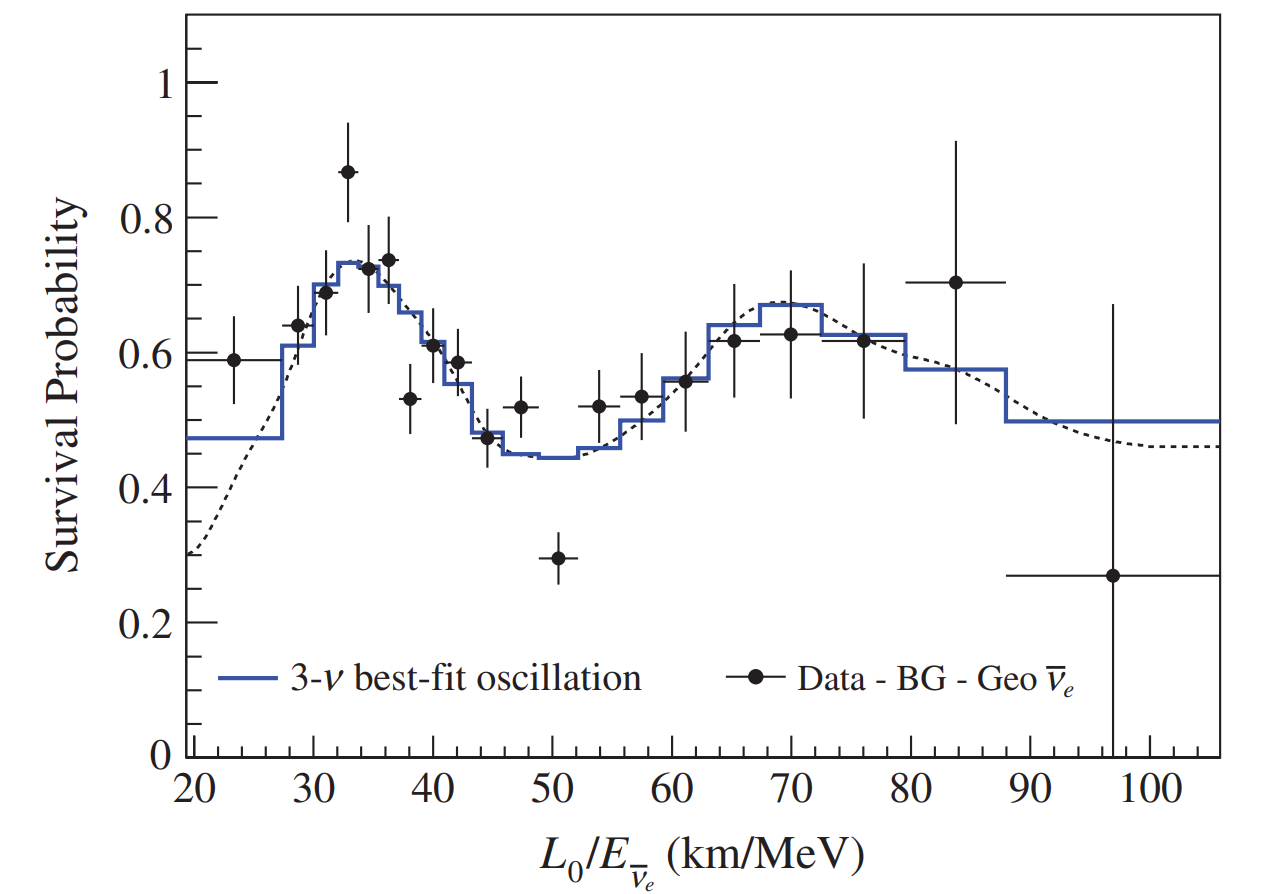
\includegraphics[width=0.95\linewidth]{1_NeutrinoTheory/Figs/kamland_reactor_LE_plot.png}
        \caption{}
        \label{fig:LE_plot_KamLAND_antinu}
    \end{subfigure}
    \begin{subfigure}{0.48\textwidth}
        \centering
        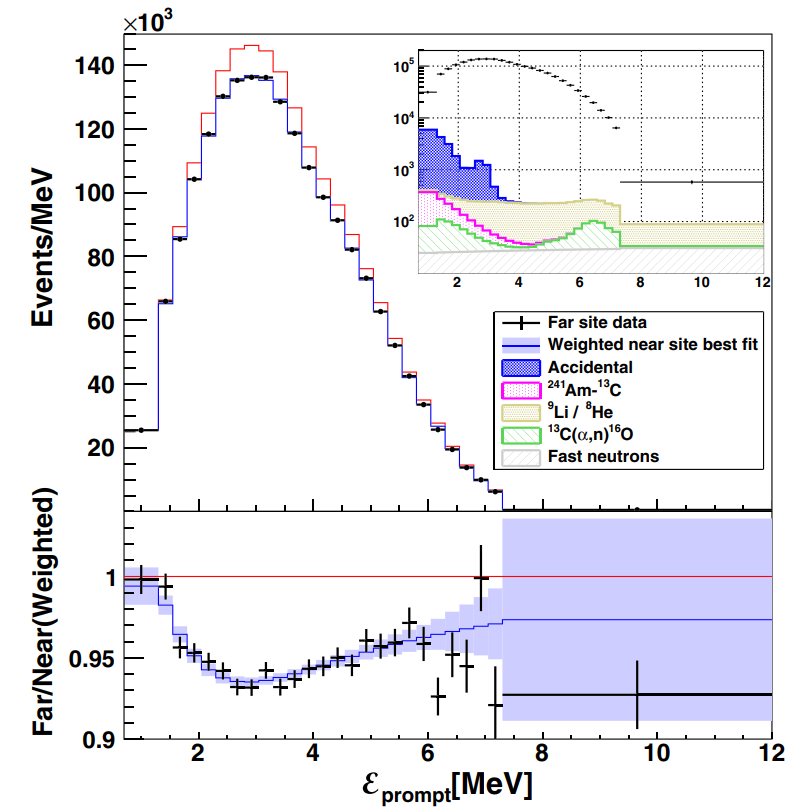
\includegraphics[width=0.95\linewidth]{1_NeutrinoTheory/Figs/dayabay_reactor_e_plot.png}
        \caption{}
        \label{fig:LE_plot_DayaBay}
    \end{subfigure}
    \begin{subfigure}{0.48\textwidth}
        \centering
        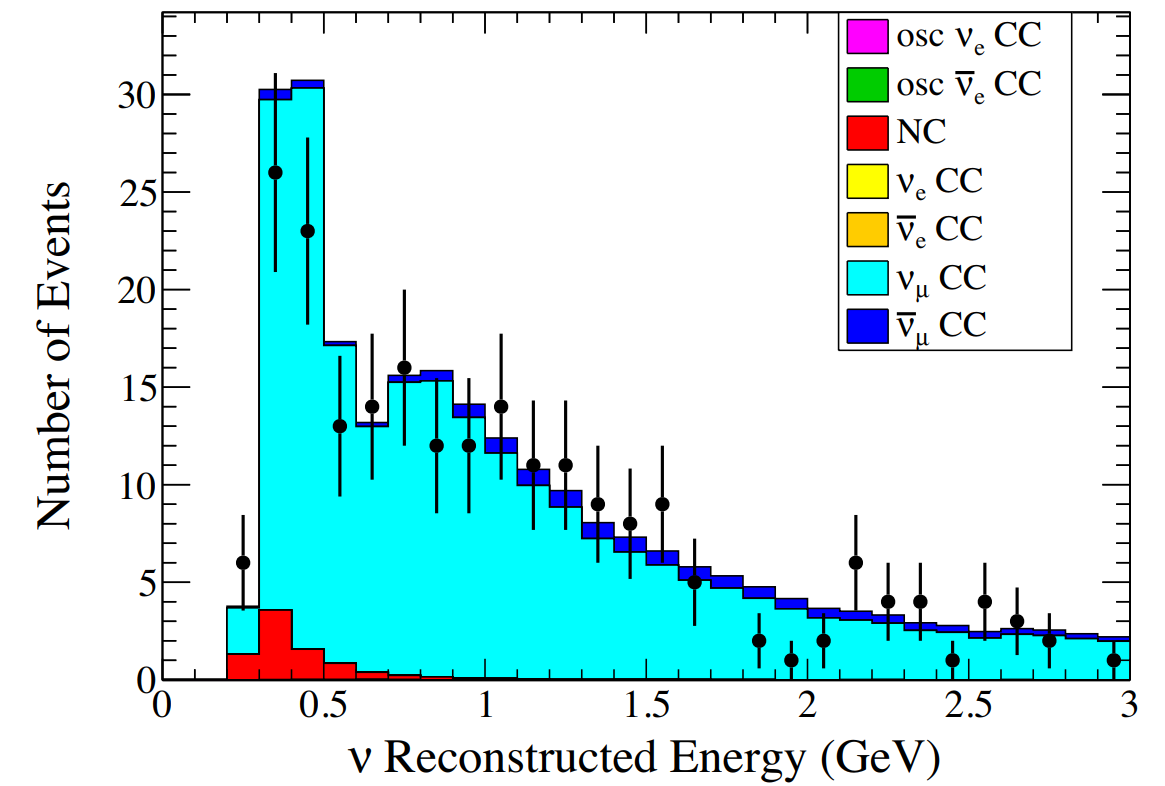
\includegraphics[width=0.95\linewidth]{1_NeutrinoTheory/Figs/T2K_numu_E_plot.png}
        \caption{}
        \label{fig:LE_plot_T2K_numu}
    \end{subfigure}
    \caption[]
    {Plots of measured survival probability for various types of neutrinos, in different experiments, as a function of $L/E$ (or just $E$ when $L$ is fixed). \textbf{(a)}: Atmospheric neutrinos from Super-Kamiokande~\cite{ashieEvidenceOscillatorySignature2004}. The solid line indicates the best-fit expectation from 2-flavour neutrino oscillations; the dashed and dotted lines correspond to the alternative hypotheses of neutrino decay and decoherence, respectively. \textbf{(b)}: Reactor anti-neutrinos from KamLAND~\cite{gandoReactorOnoffAntineutrino2013}. $L_{0} = \SI{180}{\km}$ is the flux-weighted average reactor baseline; the blue bins and black dotted line correspond to the 3-flavour neutrino oscillation best-fit curve. \textbf{(c)}: Reactor anti-neutrinos from Daya Bay~\cite{adeyMeasurementElectronAntineutrino2018}. The expected number of events in the far site with/without neutrino oscillations (blue/red lines) based on the observations in the near site is compared to observations in the far site. \textbf{(d)}: Accelerator muon neutrinos from T2K~\cite{abeImprovedConstraintsNeutrino2021}.}
    \label{fig:LE_plots}
\end{figure}

\subsubsection{Reactor Anti-neutrinos}
The detection of $\bar{\nu}_{e}$ from nuclear reactors via IBD has been used not just to first detect the existence of neutrinos by Cowan and Reines~\cite{cowanDetectionFreeNeutrino1956,reinesNeutrino1956}, but also to provide evidence for neutrino oscillations. For example, the KamLAND experiment is a large-scale liquid scintillator detector based in Japan in which IBD events can be detected~\cite{gandoReactorOnoffAntineutrino2013}. % cite KamLAND
The expected rate of these events could be derived from the known powers of the various Japanese nuclear reactors, as well as their distances from the experiment. The ratio of the measured rate to expectation as a function of $L_{0}/E$, where $L_{0}$ is the flux-averaged distance to the reactors, is shown in Fig.~\ref{fig:LE_plot_KamLAND_antinu}. The plot shows clear evidence of $\bar{\nu}_{e}$ disappearance, with an oscillatory dependence on $L_{0}/E$.

The Daya Bay~\cite{adeyMeasurementElectronAntineutrino2018}, Double Chooz~\cite{dekerretDoubleChoozTh132020}, and RENO~\cite{bakMeasurementReactorAntineutrino2018} experiments are all also liquid scintillator detectors that measured IBD interactions from reactors, but unlike KamLAND they were each placed only $\sim\SI{1}{\km}$ from a nuclear reactor. Each detector observed $\bar{\nu}_{e}$ disappearance over this much shorter length scale, also with a dependence on energy. The results from Daya Bay, as an example, are shown in Fig.~\ref{fig:LE_plot_DayaBay}. Interestingly, the magnitude of the disappearance observed in these `short-baseline' reactor antineutrino experiments is different to those seen in the `long-baseline' KamLAND experiment.

\subsubsection{Accelerator Neutrinos}
Neutrinos generated from accelerators have been able to demonstrate numerous pieces of direct evidence for neutrino oscillations. These accelerators are able to generate very high intensity beams of $\nu_{\mu}$ and $\bar{\nu}_{\mu}$, with some background of $\nu_{e}$ and $\bar{\nu}_{e}$. Much like experiments designed for reactor antineutrino measurements, accelerator neutrino detectors tend to come in two main varieties: long- and short-baseline. Typically, long-baseline experiments have two detectors, one near to the point of neutrino generation, and the much-larger far detector where the main oscillation measurements take place. The near-detector is used to ascertain the precise composition of neutrino beam, in order to minimise systematics in the composition of the beam as well as interaction cross-sections.

A wide variety of accelerator neutrino experiments have taken place over the past 25 years. The long-baseline experiments T2K and NOvA have both demonstrated disappearance of both $\nu_{\mu}$ and $\bar{\nu}_{\mu}$ from their accelerator beams with high statistical significance~\cite{abeImprovedConstraintsNeutrino2021,adamsonConstraintsOscillationParameters2017}. % cite T2K, Nova
An example of the observed energy spectrum from a predominantly $\nu_{\mu}$-type beam, as seen by T2K, is shown in Fig.~\ref{fig:LE_plot_T2K_numu}. In contrast to the energy spectrum of the neutrinos at production, which is unimodal, this plot shows oscillations in the observed rate as a function of neutrino energy. 

T2K and NOvA have also been able to observe the appearance of $\nu_{e}$ and $\bar{\nu}_{e}$ (as appropriate) in their far detectors, well above the background rate expected~\cite{abeObservationElectronNeutrino2014,adamsonFirstMeasurementElectron2016}. Recently, the two experiments have seen evidence for differences in the appearance and disappearance rates of neutrinos and antineutrinos~\cite{abeConstraintMatterAntimatter2020,aceroFirstMeasurementNeutrino2019}. % cite CP violation papers.
In addition to the appearance of $\nu_{e}$ shown by T2K and NOvA, the OPERA long-baseline neutrino experiment was able to show the appearance of $\nu_{\tau}$ in detector~\cite{agafonovaFinalResultsOPERA2018}. % cite OPERA
 
% short-baseline neutrino anomaly???

% \begin{itemize}
%     \item Describe status quo ante of massless nature of neutrinos: BEH mechanism as exists cannot allow for neutrinos to have mass as only left-handed neutrinos have been observed.
%     \item Furthermore, strong experimental limits on neutrino masses, from e.g. tritium-decay endpoint measurements by the KATRIN experiment and cosmological inferences from the CMB by the Planck satellite.
%     \item But --- then neutrino oscillations are observed over a variety of experiments and contexts. Summarise critical bits of evidence:
%     \item Electron neutrino disappearance in solar neutrino experiments, including Ray Davis' Homestake experiment, the SAGE/GALLEX experiments, and SNO. For the latter, the comparison of charged-current and neutral-current modes of interaction was clear evidence of neutrino oscillations over other types of process (e.g. neutrino decay).
%     \item Include in the above a brief description of Bahcall's Standard Solar Model.
%     \item Muon neutrino disappearance in atmospheric and long-baseline accelerator neutrino experiments, such as Super-Kamiokande, T2K, and No$\nu$a.
%     \item A few further observations to note are: reactor electron anti-neutrino disappearance from both KamLAND and Daya Bay; tau neutrino appearance at the OPERA experiment; short-baseline neutrino anomaly within LSND and MiniBooNE (with recent contrary evidence from MicroBooNE).
% \end{itemize}
% [5 pages]
\subsection{The Phenomenology of Neutrino Oscillations}\label{sec:nu_osc_phenom}
\subsubsection{Oscillations in Vacuum}\label{sec:nu_osc_phenom_vacuum}
Taken together, the observations described in the previous section naturally lead to the notion of neutrino oscillations: the idea that as neutrinos propagate through space they are capable of changing flavour. Special Relativity precludes massless particles from experiencing time evolution, so any theory of neutrinos changing flavour between one another must require non-zero mass states.

\nomenclature{\textbf{PMNS}}{Pontecorvo-Maki-Nakagawa-Sakata (neutrino mixing matrix)}
The initial theories describing neutrino oscillations were made by Pontecorvo, Maki, Nakagawa, and Sakata in the 1960s~\cite{makiRemarksUnifiedModel1962,pontecorvoNeutrinoExperimentsProblem1968}. % cite PMNS papers
These theories initially assumed a two-neutrino model of oscillations, but now that $\nu_{\tau}$ particles have been observed a three-neutrino model has been adopted. The theory starts by assuming that the flavour eigenstates of neutrinos, $\nu_{e,\mu,\tau}$ are different from the neutrino mass eigenstates, $\nu_{1,2,3}$, and are instead related to one another through the Pontecorvo-Maki-Nakagawa-Sakata (PMNS) mixing matrix, $U$:
\begin{align}
    \begin{pmatrix}
        \nu_{e} \\ \nu_{\mu} \\ \mu_{\tau}
    \end{pmatrix}
     &= U \cdot 
     \begin{pmatrix}
        \nu_{1} \\ \nu_{2} \\ \nu_{3}
    \end{pmatrix}
     = \begin{pmatrix}
        U_{e1} & U_{e2} & U_{e3} \\
        U_{\mu1} & U_{\mu2} & U_{\mu3} \\
        U_{\tau1} & U_{\tau2} & U_{\tau3} 
    \end{pmatrix} \cdot 
     \begin{pmatrix}
        \nu_{1} \\ \nu_{2} \\ \nu_{3}
    \end{pmatrix}.
    % &= \begin{pmatrix}
    %     c_{12}c_{13} & s_{12}c_{13} & s_{13}e^{-i\delta_{CP}} \\
    %     -s_{12}c_{23}-c_{12}s_{13}s_{23}e^{i\delta_{CP}} & c_{12}c_{23}-s_{12}s_{13}s_{23}e^{i\delta_{CP}} & c_{13}s_{23} \\
    %     s_{12}s_{23}-c_{12}s_{13}c_{23}e^{i\delta_{CP}} & -c_{12}s_{23}-s_{12}s_{13}c_{23}e^{i\delta_{CP}} & c_{13}c_{23} 
    % \end{pmatrix} \cdot 
    %  \begin{pmatrix}
    %     \nu_{1} \\ \nu_{2} \\ \nu_{3}
    % \end{pmatrix}.
\end{align}
Because $U$ must be unitary in order to preserve total probability, its components can be parameterised as follows:
\begin{equation}
    U = 
    \begin{pmatrix}
        c_{12}c_{13} & s_{12}c_{13} & s_{13}e^{-i\delta_{CP}} \\
        -s_{12}c_{23}-c_{12}s_{13}s_{23}e^{i\delta_{CP}} & c_{12}c_{23}-s_{12}s_{13}s_{23}e^{i\delta_{CP}} & c_{13}s_{23} \\
        s_{12}s_{23}-c_{12}s_{13}c_{23}e^{i\delta_{CP}} & -c_{12}s_{23}-s_{12}s_{13}c_{23}e^{i\delta_{CP}} & c_{13}c_{23} 
    \end{pmatrix} \cdot 
     \begin{pmatrix}
        \nu_{1} \\ \nu_{2} \\ \nu_{3}
    \end{pmatrix}.
\end{equation}
This matrix uses three ``mixing angles'' $0\leq \theta_{12},\theta_{13},\theta_{23}\leq \pi/2$, and one further parameter called the ``CP-violating phase'', $0\leq\delta_{CP}\leq2\pi$, with the abbreviations $s_{ij}=\sin{\theta_{ij}}$ and $c_{ij}=\cos{\theta_{ij}}$ used in the above expression.

Given that a neutrino flavour eigenstate $\Ket{\nu_{\alpha}(0)}$ ($\alpha=e,\mu,\tau$) is produced in some CC process at time $t = 0$, because mass eigenstates $\Ket{\nu_{i}(0)}$ ($i=1,2,3$) are simultaneously the energy eigenstates when propagating in free space, the time evolution of the neutrino state is given by:
\begin{equation}
    \Ket{\nu_{\alpha}(t)} = \sum_{i=1}^{3}U_{\alpha i}e^{-E_{i}t}\Ket{\nu_{i}(0)}.
\end{equation}
$E_{i}$ is the energy eigenvalues corresponding to the associated mass eigenstates. The oscillation probability of going from one flavour $\alpha$ to another $\beta$ is given by $P\left(\nu_{\alpha}\to\nu_{\beta}\right) = |\Braket{\nu_{\beta} | \nu_{\alpha}(t)}|^{2}$. Assuming that the neutrino is ultra-relativistic so that $E_{i}\gg m_{i}$, where $m_{i}$ is the mass of the $i^{\mathrm{th}}$ mass eigenstate, and that all mass eigenstates have the same definite momentum, one can show that the oscillation probability becomes~\cite{deppischChapterNeutrinoOscillations2019}: % cite Deppisch book?
\begin{align}\label{eq:nu_osc_vacuum}
    P\left(\nu_{\alpha}\to\nu_{\beta}\right) &=
        \delta_{\alpha\beta} 
        - 4\sum_{i<j}\Re\left\{W_{\alpha\beta,ij}\right\}\sin^{2}\left(\frac{\Delta m^{2}_{ij}L}{4E}\right)\nonumber\\
        &- 2\sum_{i<j}\Im\left\{W_{\alpha\beta,ij}\right\}\sin\left(\frac{\Delta m^{2}_{ij}L}{2E}\right),
\end{align}
where $\delta_{\alpha\beta}$ is the usual Kronecker delta, $W_{\alpha\beta,ij}=U_{\alpha i}U_{\beta i}^{*}U_{\alpha j}^{*}U_{\beta j}$, $\Delta m^{2}_{ij}=m^{2}_{i} - m^{2}_{j}$, $L$ is the distance between the creation and detection of the neutrinos, and $E_{i}\approx E$ is the average energy of the neutrino. As can be seen, the probability will oscillate as a function of $L/E$, in accordance with what was seen in Section~\ref{sec:nu_osc_evidence}.

If anti-neutrinos are produced, then oscillations are governed by $U^{*}$, which is equivalent to $U$ but with the CP phase changing sign: $\delta_{CP}\to -\delta_{CP}$. Therefore, the difference between $P\left(\nu_{\alpha}\to\nu_{\beta}\right)$ and $P\left(\bar{\nu}_{\alpha}\to\bar{\nu}_{\beta}\right)$ is given by twice the third term of Eq.~\ref{eq:nu_osc_vacuum}.

In a neutrino flavour disappearance measurement, $P_{\alpha\alpha} = P\left(\nu_{\alpha}\to\nu_{\beta}\right)$ is the \textit{survival probability} of the neutrinos. In this case, $W_{\alpha\beta,ij} = |U_{\alpha i}U_{\alpha j}^{*}|^{2}$ is real, and the survival probability formula simplifies to:
\begin{equation}
    P_{\alpha\alpha} = 1 
    - 4\sum_{i<j}|U_{\alpha i}U_{\alpha j}^{*}|^{2}\sin^{2}\left(\frac{\Delta m^{2}_{ij}L}{4E}\right).
\end{equation}

An experiment is only sensitive to neutrino oscillations from mass splitting $\Delta m^{2}_{ij}$ if $X_{ij}$ is $\mathcal{O}(1)$, where $X_{ij}$ is the phase within the relevant oscillation probability term:
\begin{equation}\label{eq:nu_osc_phase}
    X_{ij} = \frac{\Delta m^{2}_{ij} L}{4E} = 1.27 \frac{\Delta m^{2}_{ij} [10^{-3}\,\si{\eV\squared}] L [\si{\km}]}{E [\si{MeV}]}.
\end{equation}
If $X_{ij}\ll 1$, then $\sin^{2}\left(X_{ij}\right)\to 0$, and no oscillations are seen due to that mass splitting. If instead $X_{ij}\gg 1$, then what can only be observed is the average effect over many oscillations, $\left<\sin^{2}\left(X_{ij}\right)\right> = 1/2$.

From the results of a variety of neutrino oscillation experiments, the oscillation parameters and magnitudes of the mass splittings have now been measured, with varying degrees of precision. A global fit of the experimental data by the NuFit group in October 2021~\cite{estebanFateHintsUpdated2020} give the values shown in Table~\ref{tab:nufit_osc_params}. All the parameters appear to have no-zero values, implying that mixing between all neutrino flavours is possible. Furthermore, $|\dmsq{}|\ll|\Delta m^{2}_{31}|\sim|\Delta m^{2}_{32}|$, meaning there are two distinct `scales' in $L/E$ that are sensitive to neutrino oscillations.

\begin{table}
    \centering
    \begin{tabular}{c p{2.2cm} p{2.2cm}}
        \hline
        Parameter   & Normal Hierarchy                       & Inverted Hierarchy  \\ \hline \hline
        $\theta_{12} [^{\circ}]$ & $33.44^{+0.77}_{-0.74}$  & $33.45^{+0.77}_{-0.74}$     \\
        $\theta_{23} [^{\circ}]$ & $49.2^{+1.0}_{-1.3}$     & $49.5^{+1.0}_{-1.2}$  \\
        $\theta_{13} [^{\circ}]$ & $8.57^{+0.13}_{-0.12}$   & $8.60^{+0.12}_{-0.12}$  \\
        $\delta_{CP} [^{\circ}]$ & $194^{+52}_{-25}$        & $287^{+27}_{-32}$   \\
        $\dmsq{} [10^{-5}\,\si{eV\squared}]$ & $7.42^{+0.21}_{-0.20}$ & $7.42^{+0.21}_{-0.20}$    \\
        $\Delta m^{2}_{3\ell} [10^{-3}\,\si{eV\squared}]$ & $+2.515^{+0.028}_{-0.028}$ & $-2.498^{+0.028}_{-0.029}$    \\
        \hline
    \end{tabular}
    \caption[Global Fit neutrino oscillation parameters]
    {Global fit results for the neutrino oscillation parameters and mass splittings, as performed in NuFit 5.1~\cite{estebanFateHintsUpdated2020}. The results for both the Normal and Inverted Hierarchy are shown: $\Delta m^{2}_{3\ell} = \Delta m^{2}_{31}$ in the former, $\Delta m^{2}_{32}$ in the latter. The results used do not include atmospheric neutrino data from Super-Kamiokande.}
    \label{tab:nufit_osc_params}
\end{table}

\nomenclature{\textbf{IH}}{Normal Hierarchy (of neutrino masses)}
\nomenclature{\textbf{NH}}{Inverted Hierarchy (of neutrino masses)}
In addition to this information, we also know from solar data that the sign of \dmsq{} must be positive, for reasons that will be explained in the next section. However, the same cannot be yet said for $\Delta m^{2}_{31}$. This leads to two possible scenarios of the ordering of the neutrino mass states. If the sign of $\Delta m^{2}_{31}$ is positive, then $m_{\nu_{1}}<m_{\nu_{2}}<m_{\nu_{3}}$, known as the Normal Hierarchy (NH). Alternatively, $m_{\nu_{3}}<m_{\nu_{1}}<m_{\nu_{2}}$, known as the Inverted Hierarchy (IH).

\subsubsection{Neutrino Oscillations in Matter}
Considering only neutrino oscillations in vacuum is insufficient to understanding the results of certain neutrino experiments, especially those detecting high-energy solar neutrinos, such as those from the \beight{} chain. Using Eq.~\ref{eq:nu_osc_phase} for the case of solar neutrinos, one finds that $X_{ij}\gg 1$ for all $i,j$, so all effects of neutrino oscillations in the vacuum should be washed out. This leads to an expected electron neutrino survival probability for solar neutrinos of:
\begin{align}\label{eq:solar_pee_naive}
    P_{ee}  &= 1 - 2\sum_{i<j}|U_{ei}U_{ej}^{*}|^{2}\\
            &= 1 - \frac{1}{2}\sin^{2}(2\theta_{13}) - \frac{1}{2}\sin^{2}(2\theta_{12})\cos^{4}(\theta_{13})\\
            &= 0.55,
\end{align}
using the parameters in Table~\ref{tab:nufit_osc_params}. This survival probability value appears somewhat consistent with those measured in low-energy solar neutrino experiments such as SAGE and GALLEX/GNO, but not with experiments with higher energy thresholds such as Homestake, Super-Kamiokande, or SNO.

\nomenclature{\textbf{MSW effect}}{Mikheyev-Smirnov-Wolfenstein effect (of neutrinos)}
The resolution of this apparent problem is that the effect of matter on neutrino oscillations have not been considered. When neutrinos travel through a medium, the electrons, protons, and neutrons within that medium interact weakly with those neutrinos, leading to coherent forward elastic scattering. The resulting phenomenon is known as the \textit{MSW effect}, after its discovery by Mikheyev, Smirnov, and Wolfenstein~\cite{wolfensteinNeutrinoOscillationsMatter1978,mikheyevResonantAmplificationOscillations1986}. %cite MSW effect papers

One can show that there is an effective potential due to these weak interactions of the form $V_{CC}(x) = \sqrt{2}G_{F}n_{e}(x)$, where $n_{e}(x)$ is the electron number density at a position $x$~\cite{giuntiChapterNeutrinoOscillations2007}. % cite something
This effective potential is only felt by electron neutrinos, because of the additional CC interaction possible, as seen in Fig.~\ref{fig:nu_e_es_feynman_diagrams}. All neutrino flavours experience NC interactions identically, and so can be ignored in what follows. The effective potential modifies the Hamiltonian, and therefore by the Schr\"{o}dinger Equation the propagation of the neutrino wavefunctions are modified.

The resulting dynamics of the MSW effect for 3-$\nu$ oscillations in a general medium can become quite complex. However, for the case of solar neutrinos two simplifying assumptions can be made that make many of the equations far more tractable: a full discussion can be read in e.g.~\cite{giuntiChapter13Phenomenology2007}. % cite Giutti
Firstly, for solar neutrinos it can be shown that $A_{CC} = 2EV_{CC} \ll \Delta m^{2}_{31}$, leading to the evolution of the $\nu_{3}$ state decoupling from the $\nu_{1}$ and $\nu_{2}$ states. There exists a new basis in which the Hamiltonian is diagonalised, known as the matter eigenstate basis, leading to new effective oscillation parameters: %cite Giutti
\begin{align}\label{eq:matter_osc_params}
    \tan{2\theta_{12}^{M}} &= \frac{\tan{2\theta_{12}}}{1-\frac{A_{CC}}{A_{res}}},\nonumber\\
    \Delta m^{2}_{M,21} &= \dmsq{}\sqrt{\sin^{2}2\theta_{12} + \cos^{2}2\theta_{12}\left(1-\frac{A_{CC}}{A_{res}}\right)^{2}},\\
    A_{res} &= \frac{\cos{2\theta_{12}\dmsq{}}}{\cos^{2}\theta_{13}}.\nonumber
\end{align}
$A_{res}$ is the value of $A_{CC}$ at which a resonance occurs, leading to the effective mass splitting $\Delta m^{2}_{M,21}$ being minimised. In the core of the Sun, this resonance occurs at an energy of $E\sim \SI{2}{\MeV}$. If $A_{CC} \ll A_{res}$, then the effective oscillation parameters reduce back to the vacuum oscillation parameters, as expected. If instead $A_{res} \ll A_{CC} \ll \Delta m^{2}_{31}$, then $\theta_{12}^{M}\to \pi/2$. In this case, $\nu_{e}$ that are created in the medium are completely driven into the $\ket{\nu_{2}^{M}}$ effective mass eigenstate.

Because the values of the effective oscillation parameters are a function of the electron density of the medium, calculating the full impact of the MSW effect of a medium with strongly-changing density can be challenging. However, If the rate of change of electron density is slow enough as a function of distance, a second approximation can be made: this is known as the \textit{adiabatic approximation}. For solar neutrinos, this approximation has been shown to be valid assuming the SSM and the measured values of the oscillation parameters. Under this approximation, states that are in a given effective mass eigenstate smoothly transform into one another as the neutrinos propagate. Therefore, an electron neutrino with high-enough energy that it has been driven into the $\ket{\nu_{2}^{M}}$ state in the Sun's core will then smoothly transform into the equivalent $\ket{\nu_{2}}$ mass eigenstate once it has reached the Sun's surface. This state then travels through space without any further oscillations occurring, because the neutrino has been transformed into a mass eigenstate. For such a neutrino, the detection probability becomes simply:
\begin{align}
    P(\nu_{2}\to\nu_{e}) &= |\Braket{\nu_{e}|\nu_{2}}|^{2} = |U_{e2}|^{2}\\
                         &= \sin^{2}\tonetwo{}\cos^{2}\theta_{13}\\
                         &= 0.30,
\end{align}
using the oscillation parameters from Table~\ref{tab:nufit_osc_params}. This survival probability is almost half of the value seen in Eq.~\ref{eq:solar_pee_naive}.

At intermediate energies, solar neutrinos are only partly driven into the $\ket{\nu_{2}^{M}}$ eigenstate, leading to a survival probability that is somewhere in-between the two extremes: $0.30\leq P_{ee} \leq 0.55$. The value of $P_{ee}$ for a given neutrino will be dependent on both the neutrino's energy and its location of production in the Sun: a neutrino generated closer to the core of Sun will have to travel through regions of greater electron density, driving the effective mixing angle $\theta_{12}^{M}$ larger.

Looking at data, Fig.~\ref{fig:pee_solar_data} shows the measured values of $P_{ee}$ for a number of different types of solar neutrino, each with their own characteristic energy spectrum. Also shown is the expectation after considering the MSW effect: as can be seen, the solar neutrino data appears consistent with this model.

\begin{figure}
    \centering
    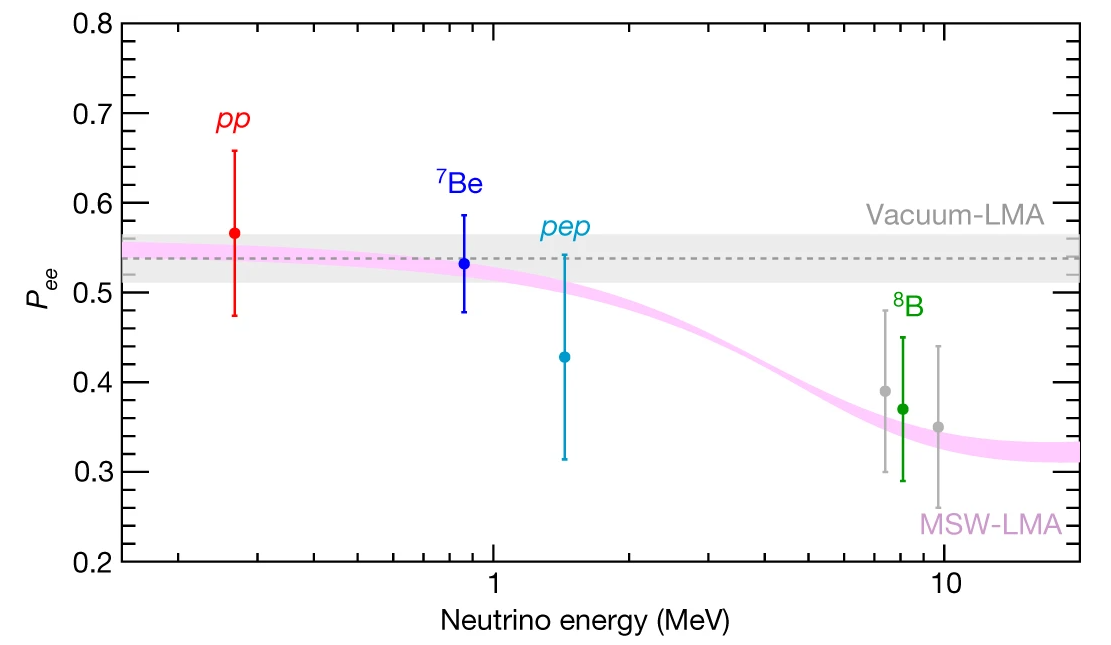
\includegraphics[width=0.8\textwidth]{1_NeutrinoTheory/Figs/borexino_pee_energy_plot.png}
    \caption[Measured survival probability versus mean neutrino energy for each solar neutrino type, as observed by Borexino]{Measured survival probability versus mean neutrino energy for each solar neutrino type, as observed by Borexino. Taken from~\cite{agostiniComprehensiveMeasurementPpchain2018}. For comparison, the expected survival probability due to vacuum oscillations and the MSW effect are shown.}
    \label{fig:pee_solar_data}
\end{figure}

Important to note is that the resonance phenomenon of the MSW effect requires a positive sign for \dmsq{} to occur, given that $0\leq\tonetwo{}\leq\pi/4$. If $\dmsq{}<0$, then in the case where $|A_{CC}|\gg |A_{res}|$, $\theta_{12}^{M}$ will be driven to 0 instead of $\pi/2$. This would lead to the survival probability of solar neutrinos increasing at higher energies, entirely counter to what is seen in data. Because of this, the sign of \dmsq{} is known to be positive.

% \begin{itemize}
%     \item Describe the current phenomenological model of 3-flavour neutrino oscillations that can explain all of this evidence: the PMNS mixing matrix.
%     \item Describe also the MSW effect, which is critical for explaining solar neutrino oscillations.
%     \item Show the formula for solar neutrino oscillations, given this MSW effect in both the Sun and Earth. Note the dependence of solar neutrino oscillations on only the ``solar'' oscillation parameters. This is all particularly useful for the solar analysis chapter.
% \end{itemize}
% [3 pages]

\subsection{The Origins of Neutrino Mass}
Having seen a wide variety of experiments over many decades observe neutrino oscillations, and the phenomenology that describes them requiring at least two neutrino mass states to be non-zero, a critical question is how neutrino masses can be included into the SM. There are two different approaches to doing so. If neutrinos are given a \textit{Dirac mass term}, then a term similar to the one in Eq.~\ref{eq:SM_yukawa_leptons} is added, now using right-handed neutrino terms $\nu^{c}_{j}$:
\begin{align}
    -\mathcal{L}_{\mathrm{Dirac}} &= \sum_{i,j}y^{\nu}_{ij}\bar{L}^{i}CH\nu^{c}_{j} + \mathrm{ h.c.}\\
                              &\to \sum_{i,j}m^{\nu}_{ij}\bar{\nu}_{i,L}\nu^{c}_{j} + \mathrm{ h.c.}.
\end{align}
The $3\times3$ matrix $y^{\nu}_{ij}$ describes the Yukawa coupling strengths between the neutrinos and the charge conjugate of the Higgs doublet, $CH$. After SSB, a neutrino mass matrix is obtained $m^{\nu}_{ij} = \frac{v}{\sqrt{2}}y^{\nu}_{ij}$, which can be related to the PMNS mixing matrix~\cite{deppischChapterNeutrinosStandard2019}. %cite
The theoretical downsides of this approach are two-fold: firstly, because $v = \SI{246.22}{\GeV} \gg m_{\nu_{i}}\sim \mathcal{O}(10^{-2}\si{\eV\squared})$, this requires fine-tuning of the Yukawa coupling parameters down to values $\sim\mathcal{O}(10^{-14})$.

A second assumption needed for neutrinos to be Dirac particles is the existence of right-handed, `sterile' neutrinos. These are so-called because their right-handed nature precludes them from interacting via any of the three main fundamental forces of particle physics. The only known means by which sterile neutrinos could have any contact with the rest of the SM is via the above mass term of the Lagrangian; this implies that neutrinos could oscillate into a sterile neutrino state, for example. The LSND and MiniBooNE short-baseline neutrino experiments have seen excesses at low energies that could be explained by oscillations of a sterile neutrino with a mass splitting of $\Delta m^{2}_{41}\sim\mathcal{O}(\SI{1}{\eV\squared})$~\cite{aguilarEvidenceNeutrinoOscillations2001,aguilar-arevaloUpdatedMiniBooNENeutrino2021}; % cite LSND & MiniBooNE excess papers
however, these results seem at odds with recent results by the MicroBooNE Collaboration~\cite{abratenkoFirstConstraintsLight2023}. % cite MicroBooNE

\nomenclature{\textbf{BSM}}{Beyond the Standard Model}
An alternative approach to generating neutrino masses without needing to posit the existence of right-handed neutrino states is through a \textit{Majorana mass term}:
\begin{equation}
    \mathcal{L}_{M} = \frac{1}{2}\sum_{i,j}m^{\nu}_{ij}\nu^{T}_{i,L}C\nu_{j,L} + \mathrm{ h.c.},
\end{equation}
where there is now no longer a coupling to the Higgs field, and instead the charge conjugate of the left-handed neutrino states is used. This term breaks SM gauge symmetry, so in theories Beyond the Standard Model (BSM) that want to include such a term typically introduce a higher-order term that reduces after SSB down to the Majorana term~\cite{weinbergBaryonLeptonNonconservingProcesses1979}. % cite some relevant papers, inc. Weinberg
Many of these BSM theories, for example ones that include a so-called `Seesaw Mechanism', also have a means of explaining why neutrinos have such light masses, without having to resort to `unnatural' Yukawa coupling strengths~\cite{minkowskiEgRateOne1977}. % cite 
For this term to exist neutrinos must be a `Majorana particle', in which they are their own antiparticle, expressed mathematically as $\nu^{c} = \nu$. This is named after Ettore Majorana, who realised that a mass term such as the above could exist under these special conditions~\cite{majoranaTeoriaSimmetricaElettrone1937}. % cite Majorana

The existence of this Majorana mass term would have major consequences, beyond just allowing for neutrino masses. Crucially, the term violates lepton number, as it allows for neutrinos to annihilate one another. Because all other terms in the SM conserve the `accidental' symmetry of lepton number conservation, any evidence of lepton number violation with neutrinos can provide strong evidence that neutrinos are Majorana particles.

\nomenclature{\textbf{\onbb{}}}{Neutrinoless double beta decay}
\nomenclature{\textbf{\twonbb{}}}{Two-neutrino double beta decay}
One prominent search mode for determining whether neutrinos have a Majorana mass term is by looking for \textit{neutrinoless double beta decay}, \onbb{}. This is a variant of the radioactive decay known as \textit{two-neutrino double beta decay}, \twonbb{}, and was first hypothesised by Wendell H Furry~\cite{furryTransitionProbabilitiesDouble1939}. % cite Furry paper
\twonbb{} is a nuclear process theorised by Maria Goeppert-Mayer~\cite{goeppert-mayerDoubleBetaDisintegration1935}, % cite
in which two $\beta$-decays occur simultaneously in one nucleus, generating two electrons and two electron anti-neutrinos. This is only possible in the subset of isotopes for which \twonbb{} is energetically favourable, but the usual single $\beta$-decay is not (or indeed any other form of nuclear decay).

One example of an isotope capable of \twonbb{} is \ce{^{130}Te}. Fig.~\ref{fig:bb_isobar_example} shows the mass excesses of the nuclear ground state energy levels for isotopes in the isobar $A = 130$. As can be seen, \ce{^{130}Te} is not capable of $\beta^{-}$-decay to \ce{^{130}I}, but decay via \twonbb{} down to the stable isotope \ce{^{130}Xe} is possible. This process has been observed by the CUORE experiment~\cite{adamsMeasurementEnsuremathNu2021}, % cite CUORE
and \twonbb{} has been similarly observed in a number of other isotopes such as \ce{^{76}Ge}~\cite{agostiniResultsBetaBeta2015}, % cite
\ce{^{136}Xe}~\cite{gandoPrecisionAnalysis1362019}, % cite
and \ce{^{150}Nd}~\cite{arnoldMeasurementEnsuremathNu2016}. % cite

\begin{figure}[!th]
    \centering
    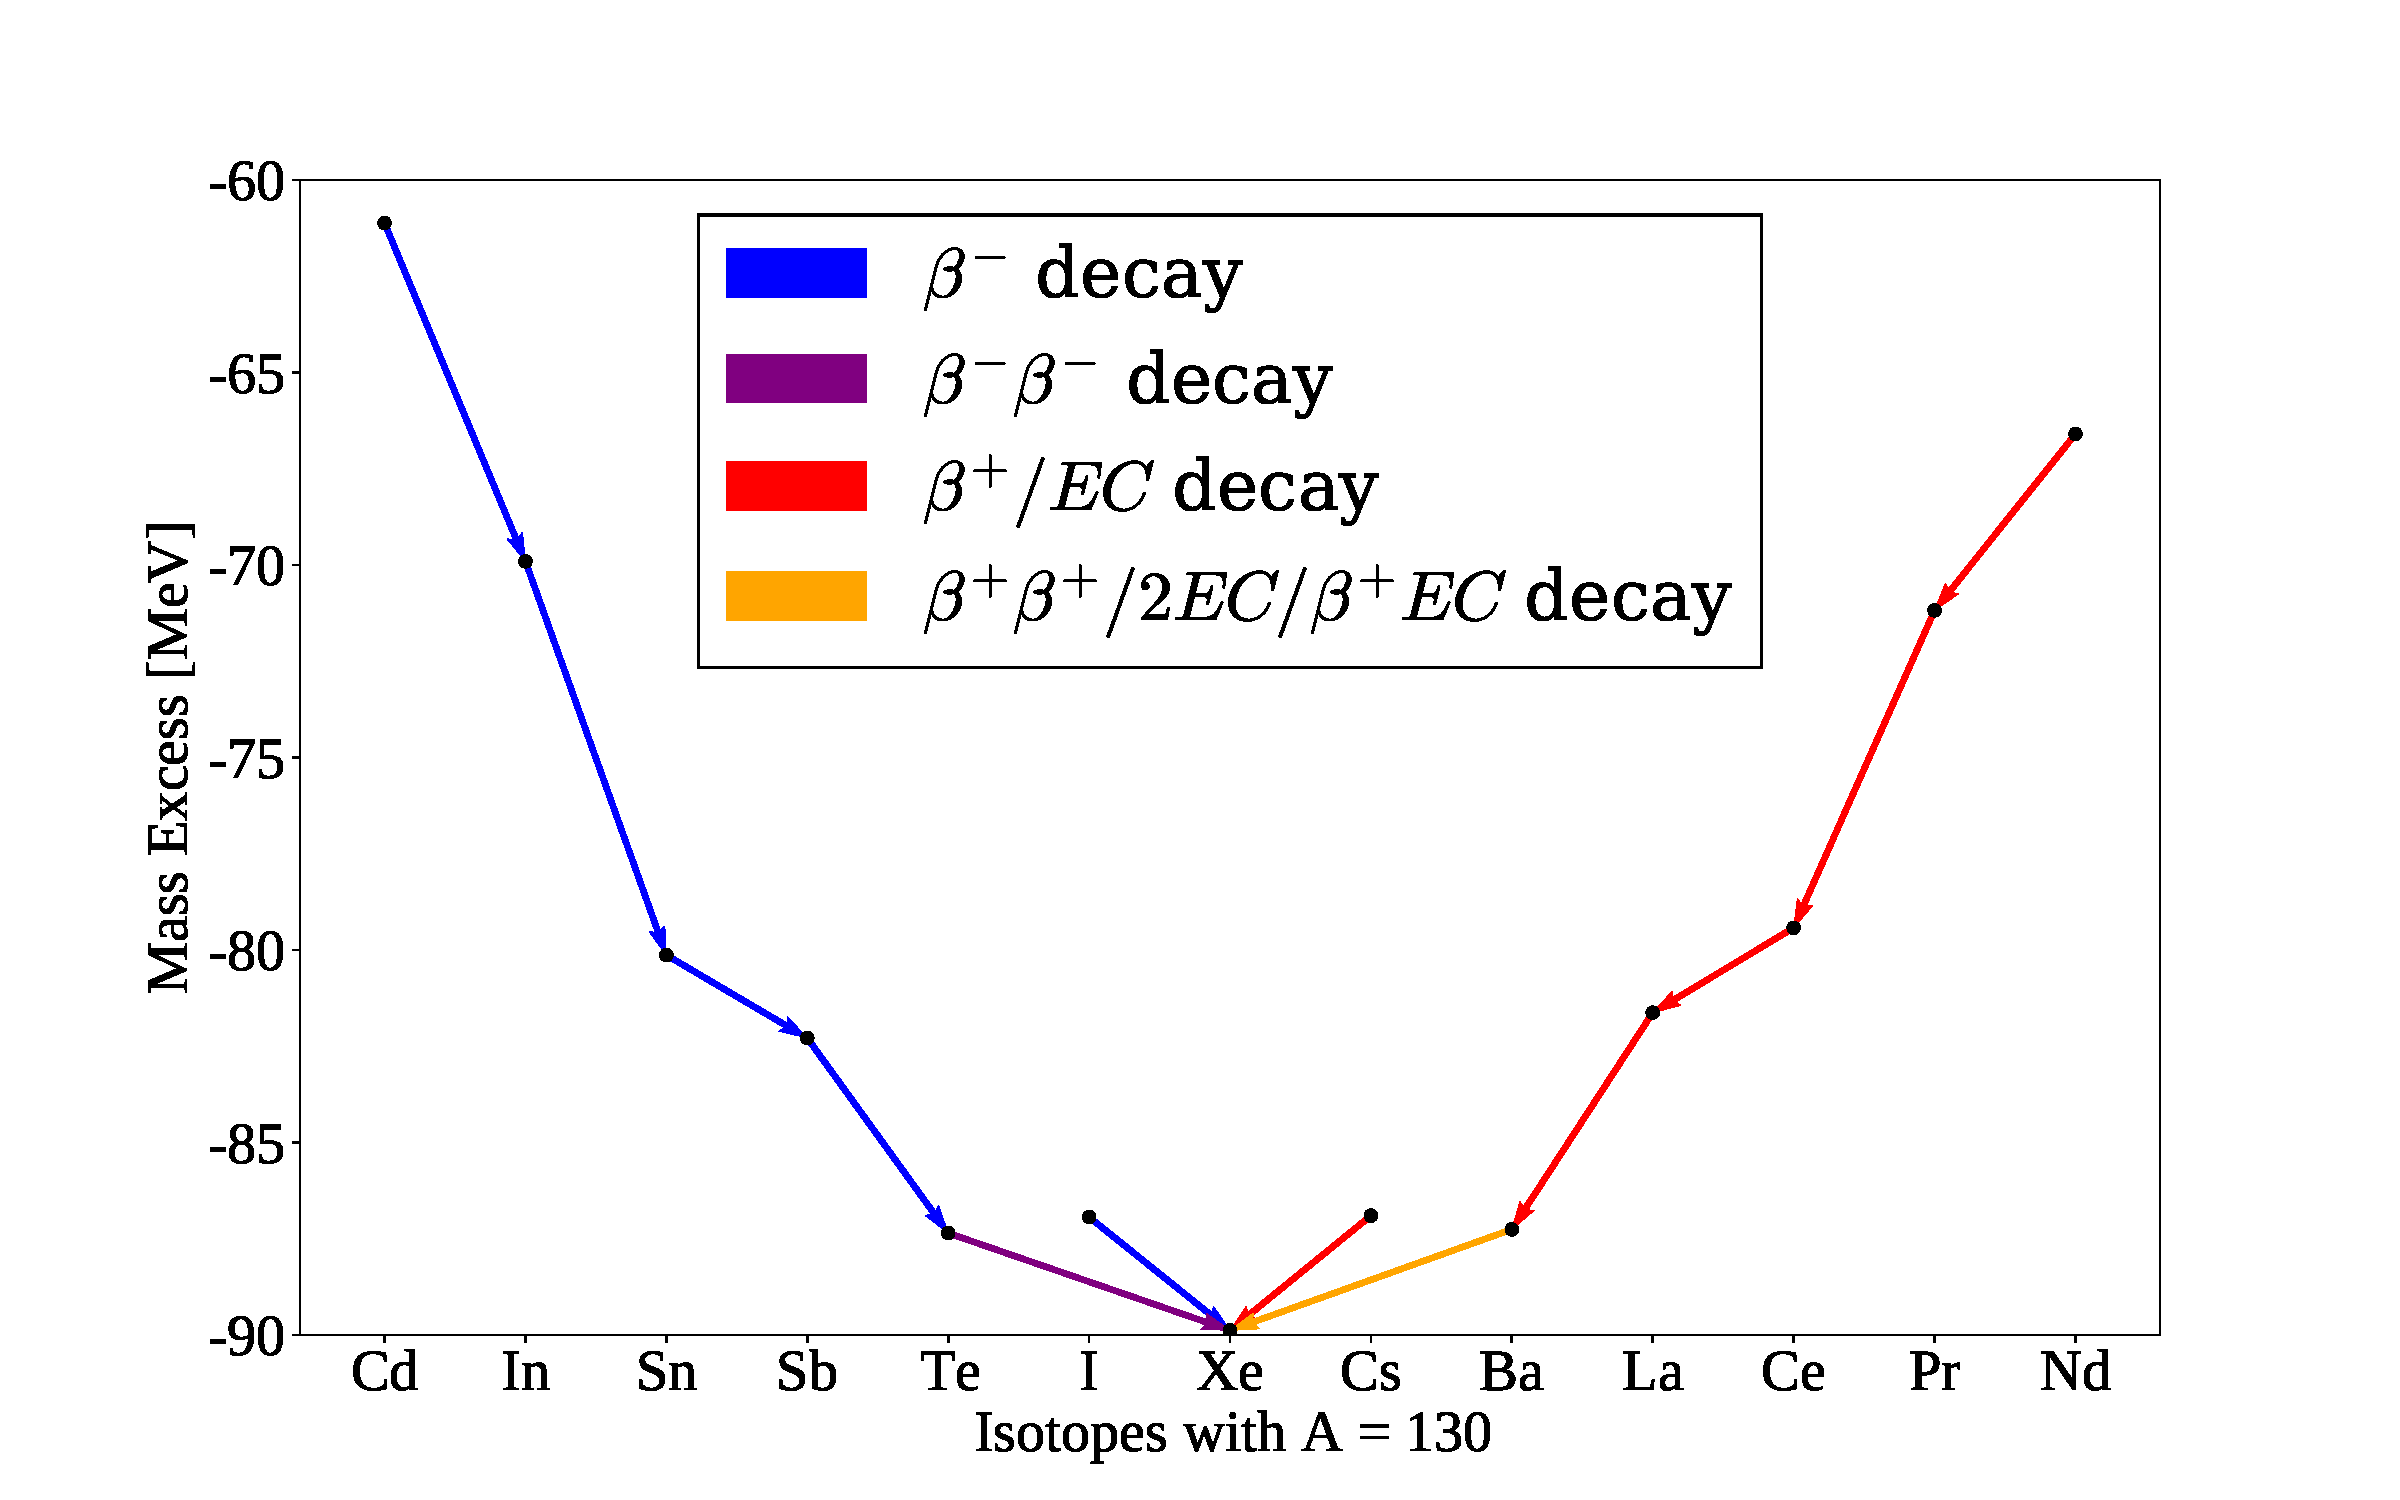
\includegraphics[width=0.8\textwidth]{1_NeutrinoTheory/Figs/A_130_isobars.pdf}
    \caption[]{Masses excesses of the $A = 130$ isobar, from~\cite{kondevNuclearDataSheets2008}. The allowed weak decays between isotopes are shown by coloured arrows; note how both \ce{^{130}Te} and \ce{^{130}Ba} can only decay via second-order weak processes.}
    \label{fig:bb_isobar_example}
\end{figure}

Unlike \twonbb{}, \onbb{} would emit no neutrinos during the decay, and instead a virtual anti-neutrino emitted by one nucleon would be captured on another as a neutrino. Fig.~\ref{fig:feynman_diagram_ovbb} shows a Feynman diagram for this process. A theorem by J. Schechter and J.W.F. Valle~\cite{schechterNeutrinolessDoubleDecay1982} % cite
says that, as long as the weak interaction is governed by some form of local gauge theory, any observation of \onbb{} guarantees the existence of a Majorana mass term for neutrinos.

\begin{figure}[!th]
    \centering
    \begin{subfigure}{0.40\textwidth}
        \centering
        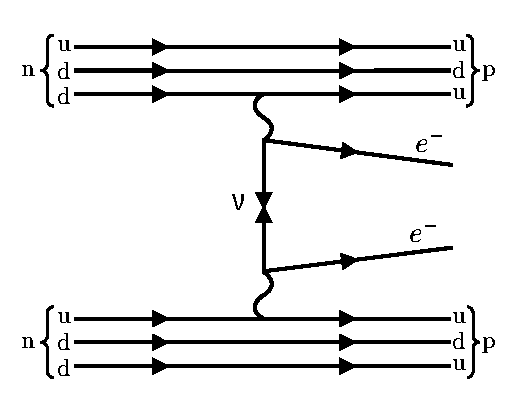
\includegraphics[width=0.95\linewidth]{1_NeutrinoTheory/Figs/feynman_diag_ovbb.pdf}
        \caption{}
        \label{fig:feynman_diagram_ovbb}
    \end{subfigure}
    \begin{subfigure}{0.59\textwidth}
        \centering
        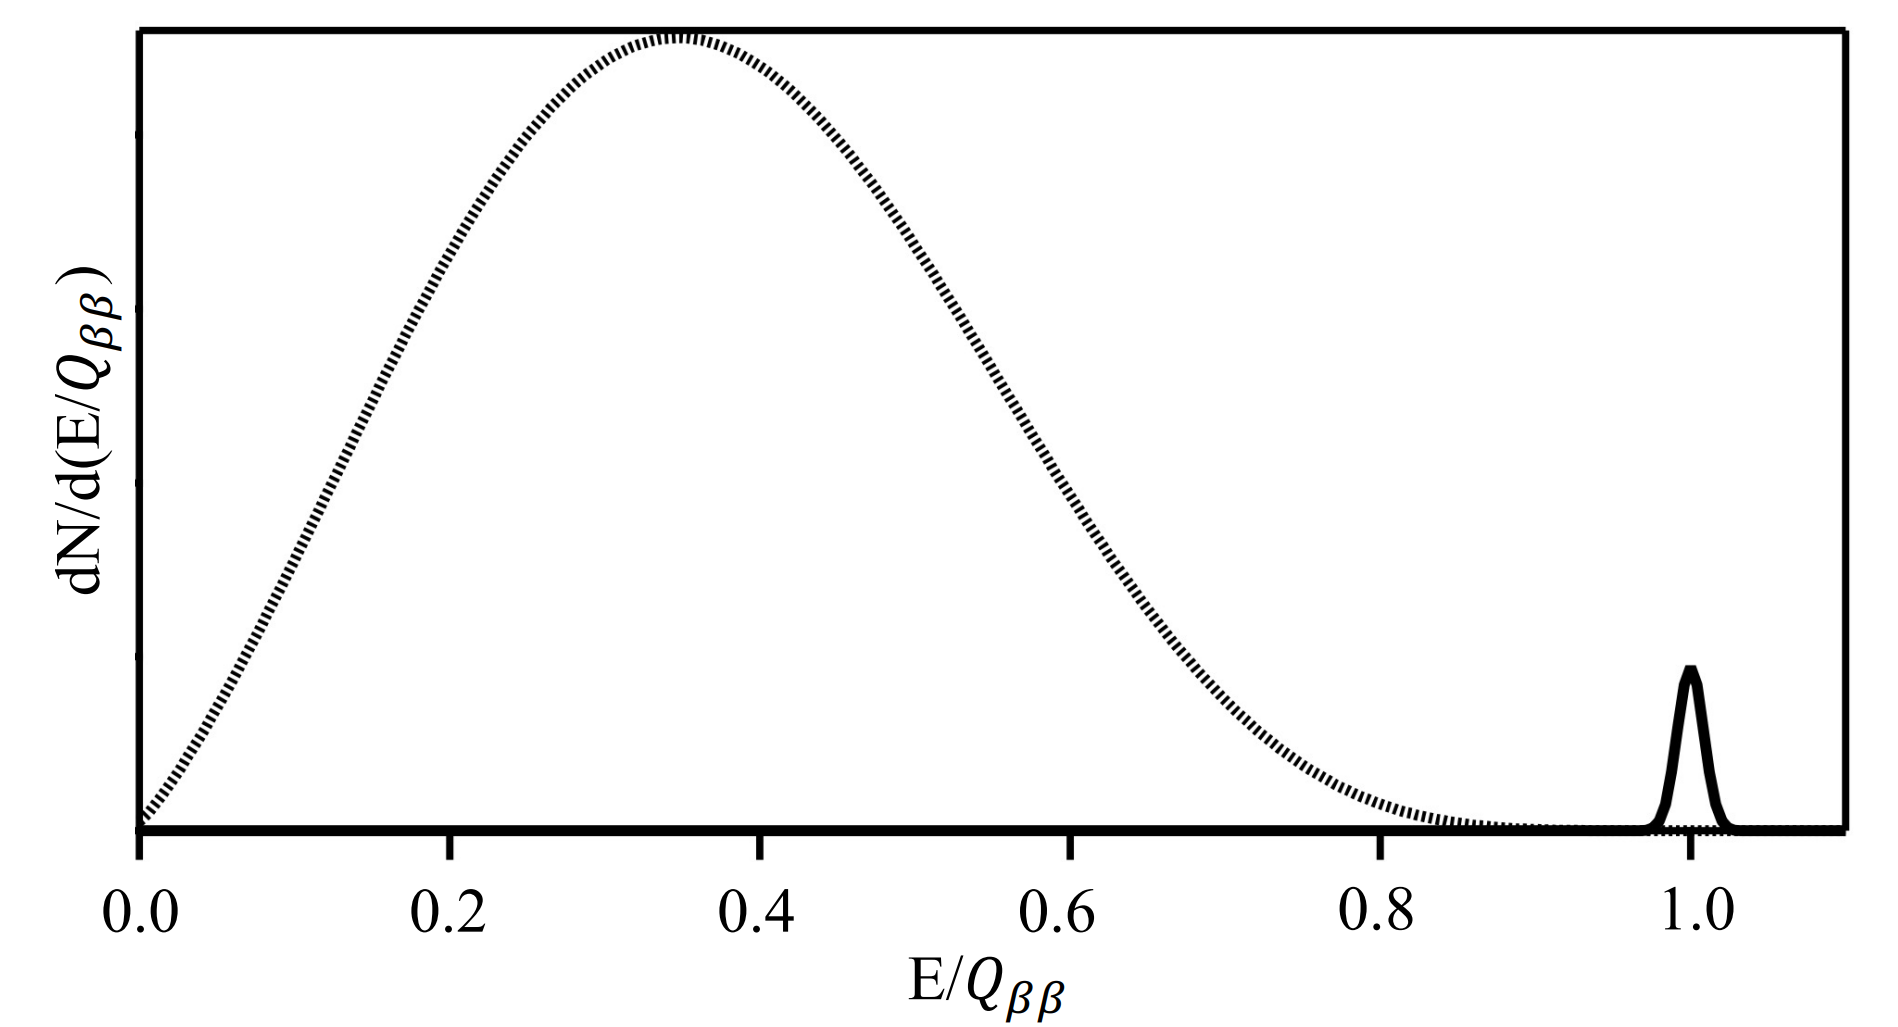
\includegraphics[width=\linewidth]{1_NeutrinoTheory/Figs/0vbb_2vbb_energy_spectrum_comparison.png}
        \caption{}
        \label{fig:energy_spectrum_bb}
    \end{subfigure}
    \caption[]
    {\textbf{(a)}: Feynman diagram for \onbb{} decay. \textbf{(b)}: Sketch of the energy spectra for \twonbb{} (dashed line) and \onbb{} decays (solid line). The $Q$-value of the decay is written here as $Q_{\beta\beta}$. Taken from~\cite{inacioDataAnalysisWater2022}.}
    \label{fig:ovbb_plots}
\end{figure}

The lack of neutrinos generated in \onbb{} compared to \twonbb{} enables a method for distinguishing between the two processes. In \twonbb{}, the energy of the decay is shared between the two electrons and two anti-neutrinos generated. Given that the anti-neutrinos rarely ever interact, the observed energy of the event will come only from the electrons (ignoring the negligble kinetic energy of the daughter nucleus). This leads to a broad observed energy spectrum. In comparison, with \onbb{} all the decay energy is passed onto the electrons, and so the observed energy spectrum will be a thin peak at the $Q$-value of the decay. This is shown schematically in Fig.~\ref{fig:energy_spectrum_bb}. As can be seen, \onbb{} can be searched for by looking for an excess of radioactive decay events generated by a \twonbb{}-decaying isotope at the $Q$-value.

No evidence of \onbb{} has been seen at the time of writing. However, numerous experiments have been searching for the decays in a variety of isotopes, and more are under construction or being planned. A summary of the current state of searches for the most prominent isotopes that could theoretically allow \onbb{} is shown in Table~\ref{tab:ovbb_current_limits}. In absence of an observation, experiments report a limit on the minimum possible half-life of \onbb{}, $T_{1/2}^{\onbb{}}$. If \onbb{} is observed, the measured half-life can be used to help determine the neutrino masses, through the formula:
\begin{equation}
    \frac{1}{T_{1/2}^{\onbb{}}} = \frac{ |m_{\beta\beta}|^{2}}{m_{e}^{2}}G_{\nu}|\mathcal{M}_{\onbb{}}|^{2},
\end{equation}
where $G_{\nu}$ and $\mathcal{M}_{\onbb{}}$ are the phase space factor and matrix elements of the decay, and $m_{\beta\beta}$ is known as the `effective \onbb{} mass', defined as:
\begin{equation}
    m_{\beta\beta} = \sum_{i=1}^{3}U_{ei}^2m_{\nu_{i}}.
\end{equation}

\begin{table}[!th]
    \centering
    \begin{tabular}{c p{3.0cm} p{4.0cm} p{0.7cm}}
        \hline
        Isotope   & $T_{1/2}^{\onbb{}}$ [years] & Experiment &   \\ \hline \hline
        \ce{^{76}Ge} & $>\num{1.8e26}$  & GERDA & \cite{agostiniFinalResultsGERDA2020} \\
        \ce{^{100}Mo} & $>\num{1.5e24}$  & CUPID-Mo & \cite{armengaudNewLimitNeutrinoless2021} \\
        \ce{^{130}Te} & $>\num{2.2e25}$  & CUORE & \cite{adamsSearchMajoranaNeutrinos2022} \\
        \ce{^{136}Xe} & $>\num{2.3e26}$  & KamLAND-Zen & \cite{abeSearchMajoranaNature2023} \\
        \hline
    \end{tabular}
    \caption[Current best limits on the half-life for \onbb{} decay for selected isotopes]
    {Current best limits on the half-life for \onbb{} decay, for selected isotopes. All limits given are for a 90\% CL.}
    \label{tab:ovbb_current_limits}
\end{table}

% {
% \color{blue}
% \begin{itemize}
%     \item Observed neutrino oscillations require at least two neutrino mass states to be non-zero. Given constraints of the current SM, two main ways of adding neutrino masses: a Dirac mass term (i.e. allowing for sterile neutrinos), and a Majorana mass term.
%     \item For latter, briefly describe what a Majorana particle is, and how with the Seesaw Mechanism (just the simple Type 1 described in-text) one can not only get neutrino masses but also explain their lightness relative to the other massive SM particles. Note that there exist more elaborate versions of this theory.
%     \item Furthermore, with reference to the Sakharov conditions, describe qualitatively how the Seesaw Mechanism also allows for possible leptogenesis/baryogenesis in the early Universe, and hence could explain its matter-antimatter asymmetry.
%     \item Describe briefly the nuclear physics behind double-beta decay (i.e. why it can happen at all over just normal beta decay), and then how Majorana neutrinos allow for neutrinoless double beta decay, \onbb{}.
%     \item Describe the experimental signature of \onbb{}: a spike of events of observed energy equal to the Q-value of the decay.
%     \item Note Schecter-Valle Theorem ensures that any observation of \onbb{} must be the result of neutrinos being Majorana. I.e. the Universe cannot conspire against us and have \onbb{} without Majorana neutrinos.
%     \item Very briefly note the current status of the search for \onbb{}, describing the main varieties of experimental setup seen, along with a nice canonical example of such an experiment and their best limit. In particular, the Germanium-crystal detectors such as GERDA, Xenon-TPC detectors like EXO-200, and large-scale liquid scintillators such as KamLAND-Zen.
% \end{itemize}
% [3 pages]

% [CHAPTER TOTAL: 17 pages]
% }
%!TEX root = ../thesis.tex
%*******************************************************************************
%****************************** Second Chapter *********************************
%*******************************************************************************

\chapter{The SNO+ Detector}\label{chap:detector}
\epigraph{\textit{The light-soaked days are coming.}}{\textsc{John Green}}
\section{Detector Geometry}
\nomenclature{\textbf{SNO}}{Sudbury Neutrino Observatory}
\nomenclature{\textbf{UPW}}{Ultra-pure water}
\nomenclature{\textbf{AV}}{Acrylic vessel}
\nomenclature{\textbf{PSUP}}{PMT support structure}
\nomenclature{\textbf{PMT}}{Photomultiplier Tube}
\nomenclature{\textbf{OWLs}}{Outward-looking PMTs}
The SNO+ detector is a large, multi-purpose neutrino detector built in the SNOLAB underground laboratory near Sudbury, Canada. Its main detector structure is taken from the Sudbury Neutrino Observatory (SNO)~\cite{BOGER2000172}, % cite
which can be seen in Fig.~\ref{fig:snoplus_detector}. At the heart of the detector lies the main detector medium, which changes depending on the phase of the experiment --- more on the specifics of this in Section~\ref{sec:exp_phases}. This medium is held within a \SI{12}{\metre} diameter sphere known as the Acrylic Vessel (AV). The AV floats within a body of ultra-pure water (UPW), beyond which is a stainless steel support structure (PSUP) that holds 9362 inward-facing Photomultiplier Tubes (PMTs). It is these PMTs that detect the light generated from physics events that occur within the detector medium. The AV is kept in place relative to the PSUP through a series of `hold-up' and `hold-down' tensylon ropes. All of these components are suspended within a large cylindrical cavity also filled with UPW. 91 outward-looking PMTs (OWLs) are also affixed to the outside of the PSUP, allowing for the effective vetoing of cosmic ray muons.

Directly above the detector is the Deck, within which all the detector electronics are kept. Access within the AV for calibration tools and filling is possible only through the acrylic `neck' on top of the AV. Full details of the design of the current detector can be found in~\cite{albaneseSNOExperiment2021}.

\begin{figure}
    \centering
    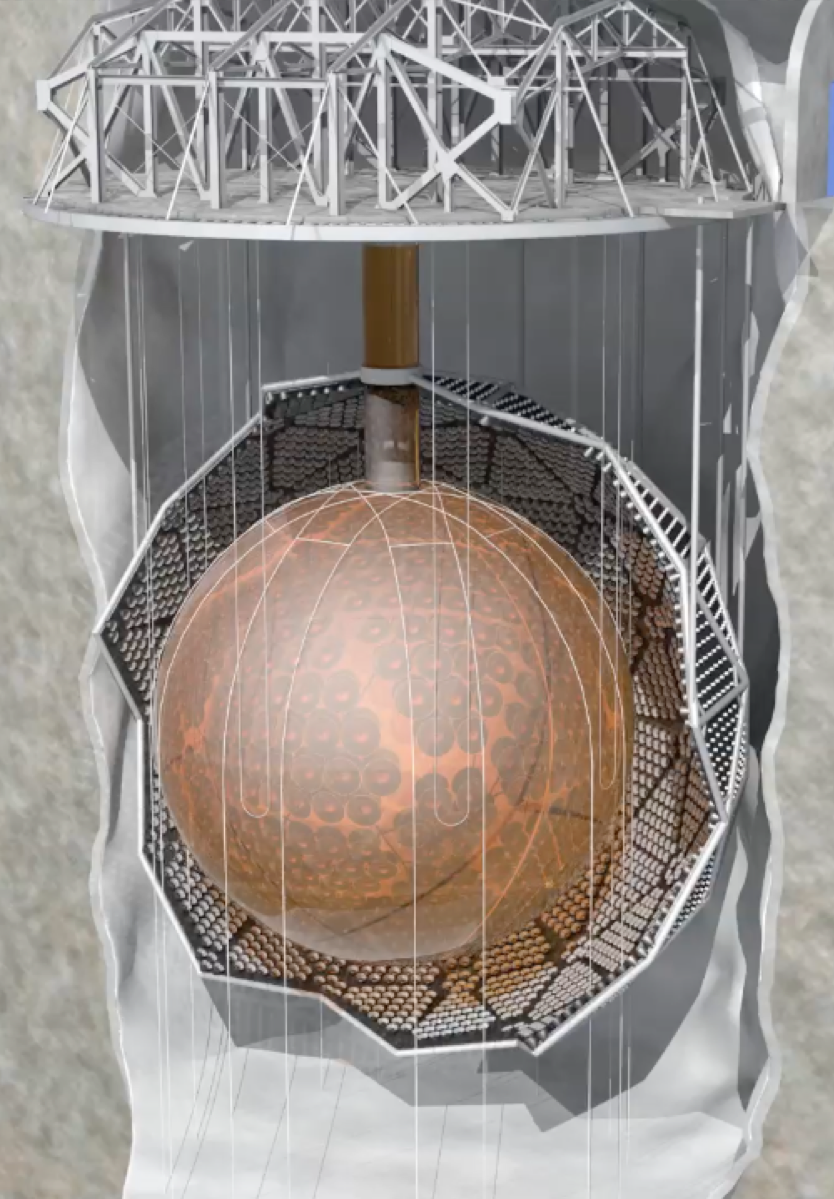
\includegraphics[width=0.48\linewidth]{2_Detector/Figs/detector_picture.png}
    \caption[3D model of the SNO+ detector]{3D model of the SNO+ detector~\cite{albaneseSNOExperiment2021}.}
    \label{fig:snoplus_detector}
\end{figure}

\section{Experimental Phases}\label{sec:exp_phases}
\nomenclature{\textbf{LAB}}{Linear alkylbenzene}
\nomenclature{\textbf{PPO}}{2,5-Diphenyloxazole}
\nomenclature{\textbf{BisMSB}}{1,4-Bis(2-methylstyryl)benzene}
\nomenclature{\textbf{DDA}}{N,N-Dimethyldodecylamine}
\nomenclature{\textbf{BD}}{1,2-Butanediol}
\nomenclature{\textbf{TeA}}{Telluric acid, \ce{Te(OH)_{6}}}
\nomenclature{\textbf{TeLS}}{Tellurium-loaded liquid scintillator}
\nomenclature{\textbf{BHT}}{Butylated hydroxytoluene}
As mentioned earlier, SNO+ was designed to fulfil a number of physics goals over multiple `phases' of the detector's lifetime. The phases are distinguished by the medium that fills the AV. The first main phase (after a brief \textbf{Air Fill Phase} used only for detector commissioning) was that of the \textbf{Water Fill Phase}, with data taken between May 2017 and July 2019. This was used to perform fundamental optical calibrations of the detector~\cite{andersonOpticalCalibrationSNO2021}, % Water optics paper
measurements of the solar neutrino flux~\cite{andersonMeasurementSolarNeutrino2019}, % water solar papers
observation of neutrino oscillations in reactor anti-neutrinos~\cite{allegaEvidenceAntineutrinosDistant2023}, % water antinu paper
and searches for nucleon decay~\cite{andersonSearchInvisibleModes2019,allegaImprovedSearchInvisible2022}. %nucleon decay papers

After this, the detector was filled with 780 tonnes of liquid scintillator known as linear alkylbenzene (LAB), mixed with the fluor 2,5-diphenyloxazole (PPO). More information on the physics of scintillators can be found in Section~\ref{sec:interactions_w_matter}. Filling of the LABPPO cocktail had to be paused in March 2020 due to the COVID-19 pandemic, leading to the detector having its bottom half still filled with UPW, and the top half filled with LAB and PPO at \SI{0.5}{\gpl}. This impromptu phase became known as the \textbf{Partial Fill}, and allowed for some creative analyses to be performed: an initial neutrino oscillation analysis from reactor anti-neutrinos~\cite{morton-blakeFirstMeasurementReactor2021}, % Iwan's thesis & forthcoming paper
as well as the first ever observation of directionality in a high light yield scintillator~\cite{patonFirstObservationDirectionality,allegaFirstObservationDirectionality}. % Josie's thesis & forthcoming PRL
Eventually, filling of the detector with liquid scintillator completed in May 2021. At that point, the concentration of PPO in the detector was at \SI{0.6}{\gpl}, markedly below the target level of \SI{2.0}{\gpl}. A further `PPO top-up' campaign then proceeded, finishing in April 2022 with a final concentration of \SI{2.2}{\gpl} PPO. Thus began the \textbf{Scintillator Phase} of the experiment, which continues on during the time of writing. The main goals for this phase include a number of solar neutrino analyses (including the one described in Chapter~\ref{chap:solar_osc_analysis}), a precision measurement of the neutrino oscillation parameter \dmsq{} using reactor anti-neutrinos~\cite{morton-blakeFirstMeasurementReactor2021}, % Iwan's thesis
and further calibrations of the detector and its backgrounds.

Finally, in the near future the detector will be loaded with Tellurium for the \textbf{Tellurium Phase}, allowing for the flagship analysis of the experiment to begin: neutrinoless double beta decay. In order to load Te within the liquid scintillator in a stable manner, a chemical loading process has been developed, as described in~\cite{autyMethodLoadTellurium2023}. % Te loading paper
The Te starts within \ce{Te(OH)_{6}} (telluric acid, otherwise known as TeA), which after purification will be reacted with 1,2-butanediol (BD) via heating and addition of N,N-Dimethyldodecylamine (DDA), which acts as a stabiliser. What results is tellurium-loaded scintillator, TeLS.

Two further chemicals are planned to be added to the scintillator cocktail. The antioxidant butylated hydroxytoluene (BHT) will be added to capture any free-radicals within the liquid scintillator, hopefully preventing any oxidation reactions that could lead to the `yellowing' of the scintillator, a degradation of its optical properties. The addition of BHT is not expected to impact the detector's optics in any substantial way. However, the other substance to also be added, 1,4-Bis(2-methylstyryl)benzene (bisMSB), will impact the optics. BisMSB acts as a `wavelength-shifter' which enables the scintillator cocktail to transmit light with a greater overall detection efficiency --- more on the details of this in Section~\ref{sec:scintillation}.

% \begin{itemize}
%     \item Describe the SNO+ geometry at a high level: explain structure, and why certain design choices were made.
%     \item Describe standard coordinate axis; note AV offset.
%     \item Mention the main phases of SNO+, both past, present, and future.
% \end{itemize}
\section{Detecting and Recording an Event in SNO+: A Journey}\label{sec:event_journey}
To understand the SNO+ detector well, it is worth thinking about how the information contained in a physics event, e.g. a solar neutrino interaction, gets observed. This section follows the journey of such an event.
\subsection{Particle Interactions with Matter}\label{sec:interactions_w_matter}
All observable physics events within the detector begin by the generation of some form of ionising radiation: $\alpha$, $\beta^{\pm}$, $\gamma$, $p$ or $n$. These can be created via numerous processes, both exciting (e.g. \onbb{} or interactions of neutrinos) and annoying (e.g. decay of background radioisotopes): see Section~\ref{sec:background_processes} for some of them. Regardless of their origin, these particles begin propagating through the detector, and interacting with the detector medium. A number of mechanisms then allow for the generation of optical-wavelength light as a result of these interactions.
\subsubsection{Cherenkov Light Emission}
Whenever a charged particle travels through a dielectric medium at speeds faster than the speed of light in that medium, light is generated from the `wake' of induced dipoles. This is known as \textbf{Cherenkov light}, a process much akin to the `sonic boom' that occurs when an object travels at supersonic speeds through a medium. This light emanates outwards in a cone along the direction of the charge's travel; the angle of the cone $\theta_{\gamma}$ being purely a function of the speed of the charged particle relative to the speed of light in vacuum, $\beta$, and the refractive index of the medium $n(\omega)$ at a given frequency $\omega$: $\cos{\theta_{\gamma}}(\omega) = \frac{1}{n(\omega)\beta}$. There is then a minimum speed necessary for Cherenkov light to be generated: $\beta_{\textrm{min}}(\omega) = 1/n(\omega)$.

In addition to the characteristic cone shape of the light, the spectrum of the light generated is also distinctive. Igor Tamm and Ilya Frank determined the expected energy $dE$ emitted per unit length travelled by the charged particle, $dx$, as~\cite{frankCoherentVisibleRadiation1937}: % Frank-Tamm formula
\begin{equation}
    \frac{dE}{dx} = 
    \frac{q^2}{c^{2}}\int_{\beta n(\omega)>1}\omega\left(1-\frac{1}{\beta^{2}n^{2}(\omega)}\right)d\omega.
\end{equation}
Here, $q$ is the charge of the moving particle. The Cherenkov emission spectrum during the water phase is shown in the black dotted line of Fig.~\ref{fig:cherenkov_scintillator_abs_emit_dist}.

\begin{figure}
    \centering
    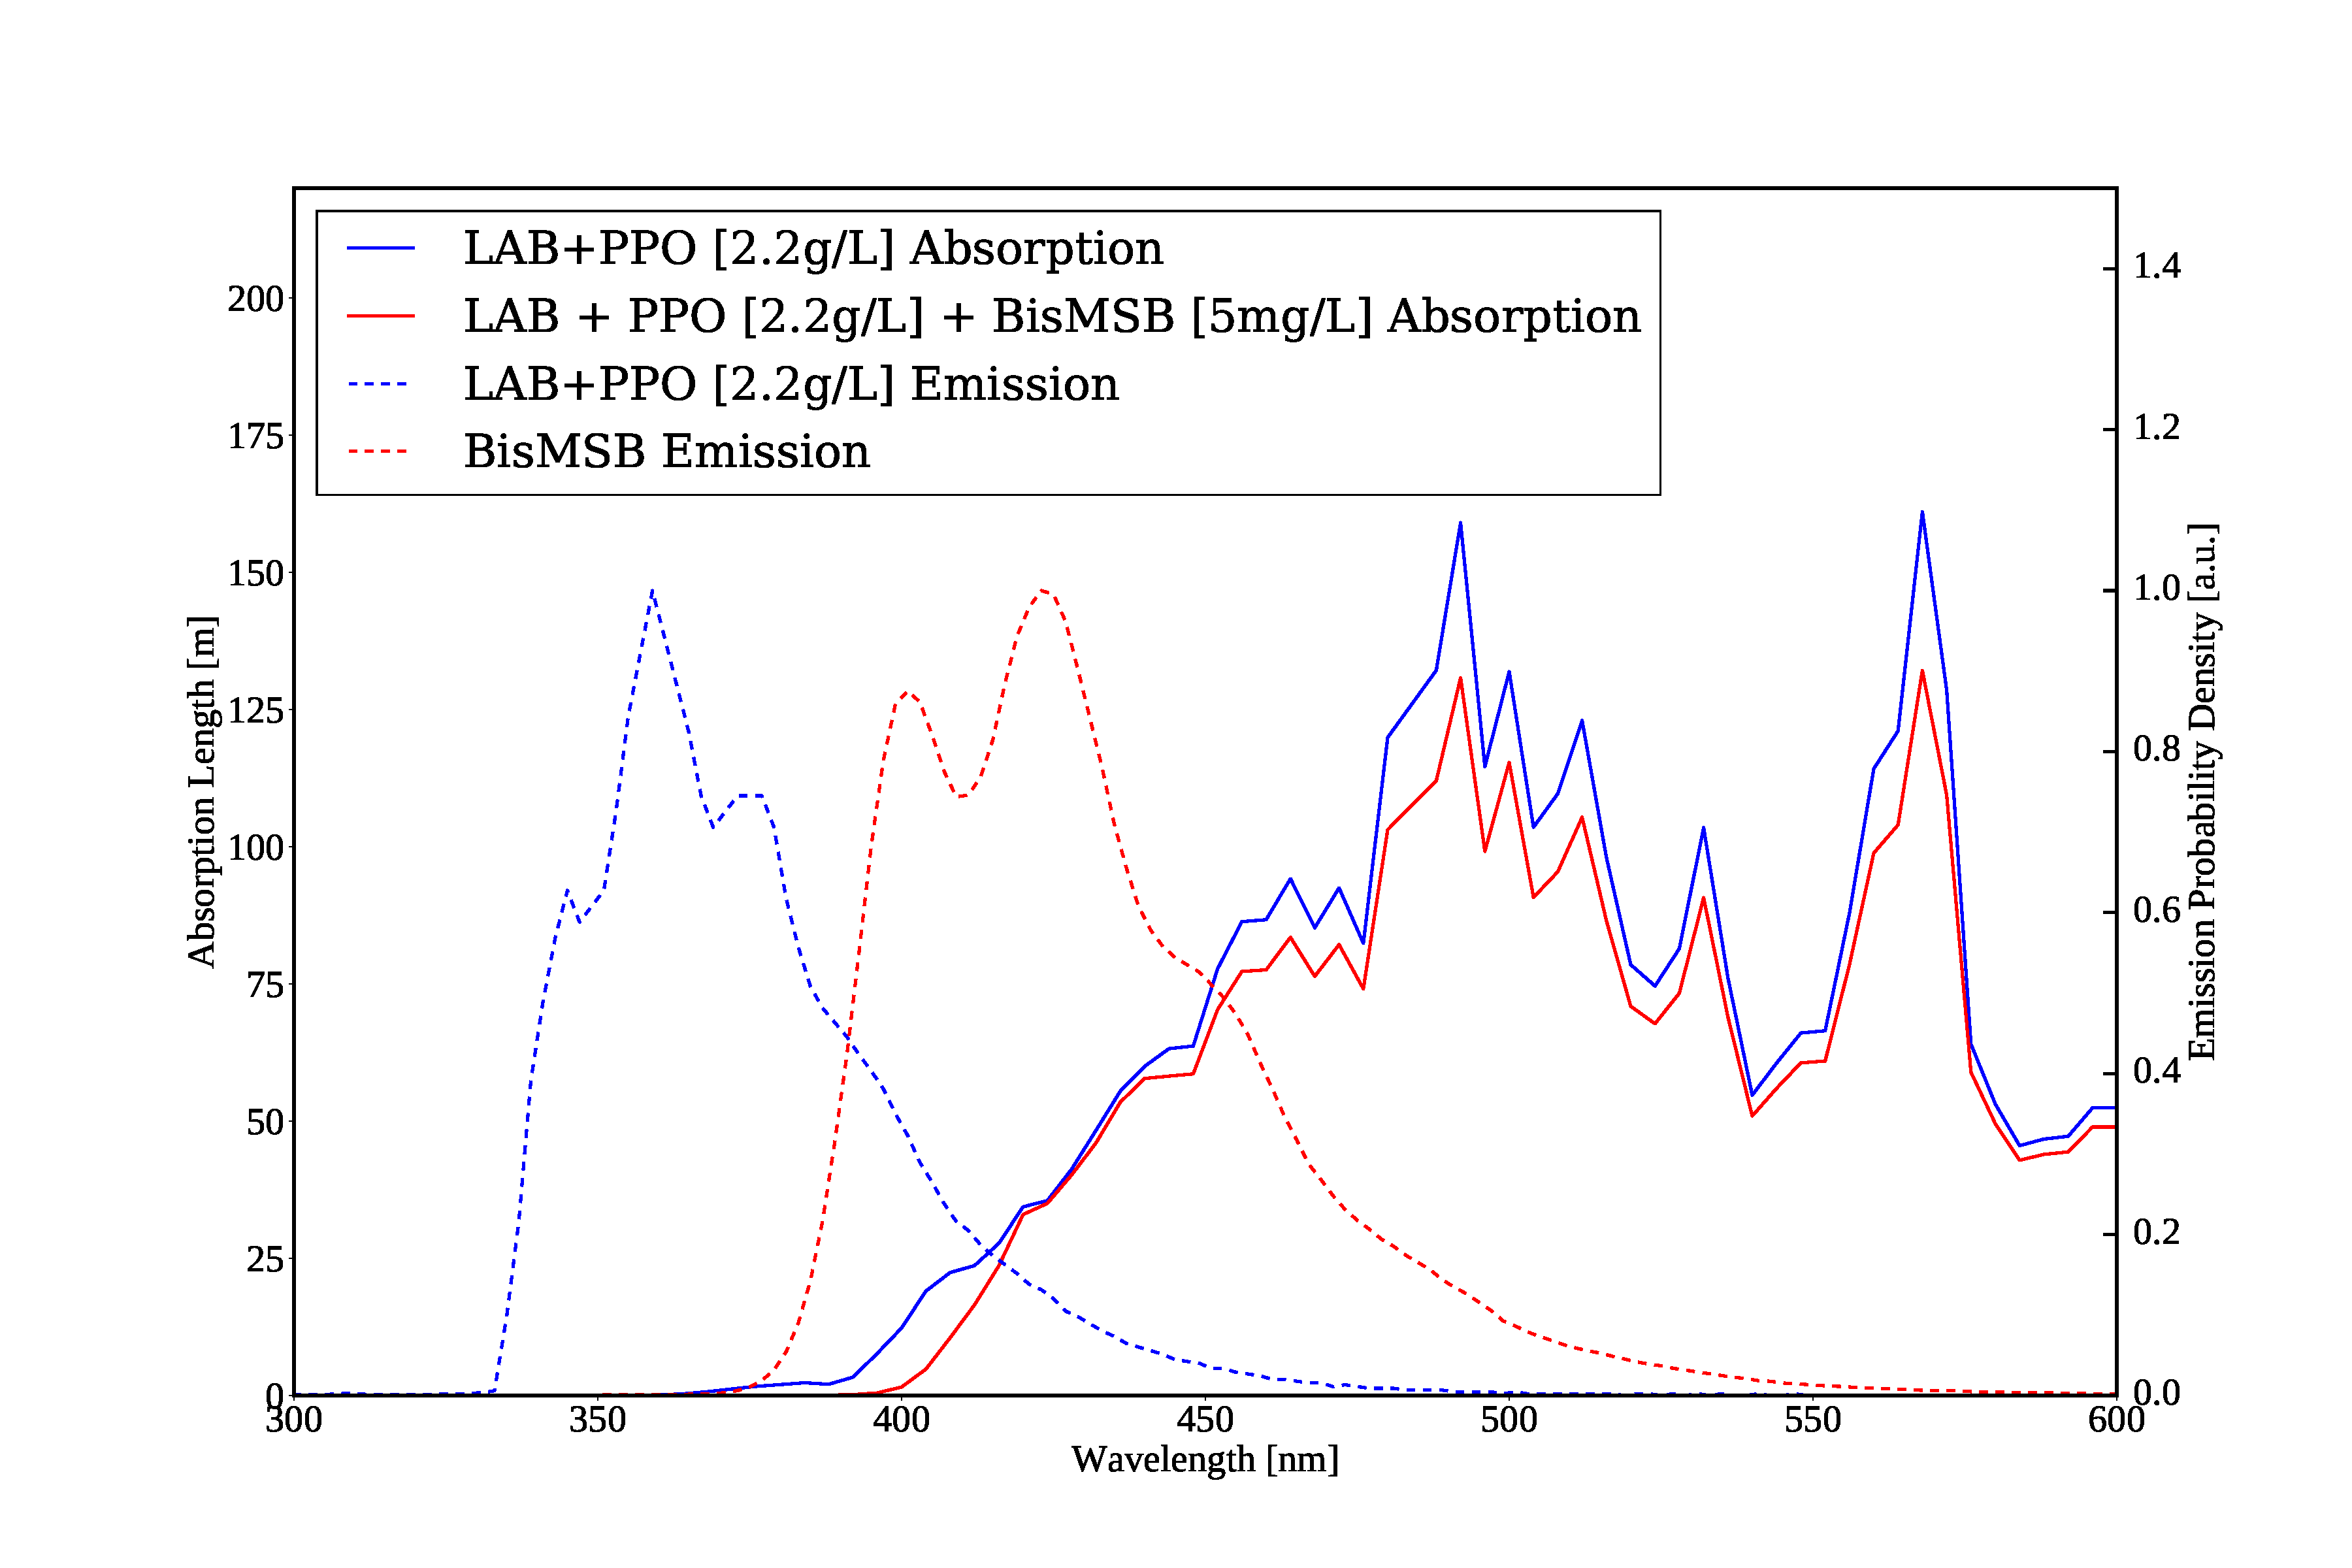
\includegraphics[width=0.8\linewidth]{2_Detector/Figs/scint_lengths_LABPPOBisMSB_plot_nice.pdf}
    \caption[Comparison of the SNO+ detector media's emission properties, versus optical phase]
    {Comparison of the SNO+ detector media's emission and absorption properties, versus optical phase~\cite{kaptanogluOpticsOverviewProposed2016,kaptanogluDocumentationAttenuationStudies2022}. % cite optics?
    }
    \label{fig:cherenkov_scintillator_abs_emit_dist}
\end{figure}

All SNO+ detection media allow Cherenkov light to be generated, as long as sufficiently high energy particles traverse it. In the water fill phase of the detector, Cherenkov light was the only means by which light could be generated. Light from Cherenkov emission can still be created in liquid scintillator, but it tends to be swamped by another form of light generation: scintillation.
\subsubsection{Scintillation}\label{sec:scintillation}
For certain special classes of material, the excitation and ionisation of atomic electrons nearby a moving charged particle can lead to the generation of optical-wavelength light, in a process known as \textbf{scintillation} (often generally referred to as `luminescence' or `fluorescence'). Although multiple varieties of scintillator exist, the one used in SNO+ is that of an organic liquid scintillator. For such liquids, scintillation light is generated from the de-excitation of delocalised electrons within carbon--carbon `$\pi$-bonds'~\cite{birksChapterScintillationProcess1967}. A major example of these $\pi$-bonds are found in benzene rings, which are present in LAB, PPO, and bisMSB.

Because of this delocalised structure, excited atomic $\pi$-electrons can stay in what is typically the first-excited state for somewhat longer than typical excited states: lifetimes of $\mathcal{O}(\SI{e-9}{\second})$ as opposed to $\mathcal{O}(\SI{e-12}{\second})$. This is what gives scintillation light its characteristic `slow' response relative to the instantaneous light generated by the Cherenkov process. Moreover, decays from this state can emit light typically in the optical-wavelength range. 
$\pi$-electrons can end up in the first-excited state either by direct excitation, or by ionisation followed by recombination. Because the ground state of these electrons are spin-singlet states, atomic spin selection rules~\cite{birksChapterScintillationProcess1967} strongly prefer any direct excitations to stay in a spin-singlet state. As a result, so-called ``inter-system crossing'' from an excited singlet state to an excited triplet state is strongly suppressed.
% In addition to excited electrons, ionised electrons can also recombine --- that is, re-enter atomic orbitals --- into various excited states, and then decay back to the ground state, also allowing for the possibility of scintillation light to be generated.

% Because of atomic spin selection rules~\cite{birksChapterScintillationProcess1967}, % cite something!
% scintillation light typically has, at the very least, a `fast' and `slow' time component.
However, ionised electrons that recombine have no such restriction, and so readily form excited triplet states. Once in such a state, the same spin selection rules strongly suppress the decay of these excited triplet electrons back down to the singlet ground state. This leads to scintillation light having, at the very least, a `fast' and `slow' time component. In SNO+, we currently model emission of scintillation light from LAB with 4 time components, following the timing distribution $f(t)$ given by:
\begin{equation}
    f(t) = \sum_{i}A_{i}\left(\frac{e^{-t/\tau_{i}}-e^{-t/\tau_{\mathrm{rise}}}}{\tau_{i}-\tau_\mathrm{rise}}\right),\; t > 0.
\end{equation}
Here, $A_{i}$ and $\tau_{i}$ correspond to the fraction of light emitted and decay constant for each component respectively, and $\tau_\mathrm{rise}$ is a common rise time. The current values for these parameters used in simulations for the emission from electron tracks can be seen in Table~\ref{tab:scint_reem_params}. These were obtained by Rafael Hunt-Stokes through the fitting of tagged \ce{^{214}Bi} $\beta$-decay events within the detector with \SI{2.2}{\gpl} LABPPO~\cite{hunt-stokesEmissionTimingTuning2022}. A plot from R. Hunt-stokes showing this fit between data and simulation is shown in Fig.~\ref{fig:typical_tres_dist_physics}.

\begin{table}
    \centering
    \begin{tabular}{c p{2cm} p{2cm}}
        \hline
        Component & $A_{i}$ & $\tau_{i}$ [ns] \\ \hline \hline
        1         & 0.665   & 7.35  \\
        2         & 0.218   & 5.45  \\
        3         & 0.083   & 117.5 \\
        4         & 0.0346  & 425   \\
        Rise      & --      & 0.8   \\
        \hline
    \end{tabular}
    \caption[Current values used to model scintillator emission from electrons in \SI{2.2}{\gpl} LABPPO]
    {Current values used to model scintillator emission from electrons in \SI{2.2}{\gpl} LABPPO~\cite{latorreNewMeasurementsTiming2016,hunt-stokesEmissionTimingTuning2022}.}
    \label{tab:scint_reem_params}
\end{table}

\begin{figure}
    \centering
    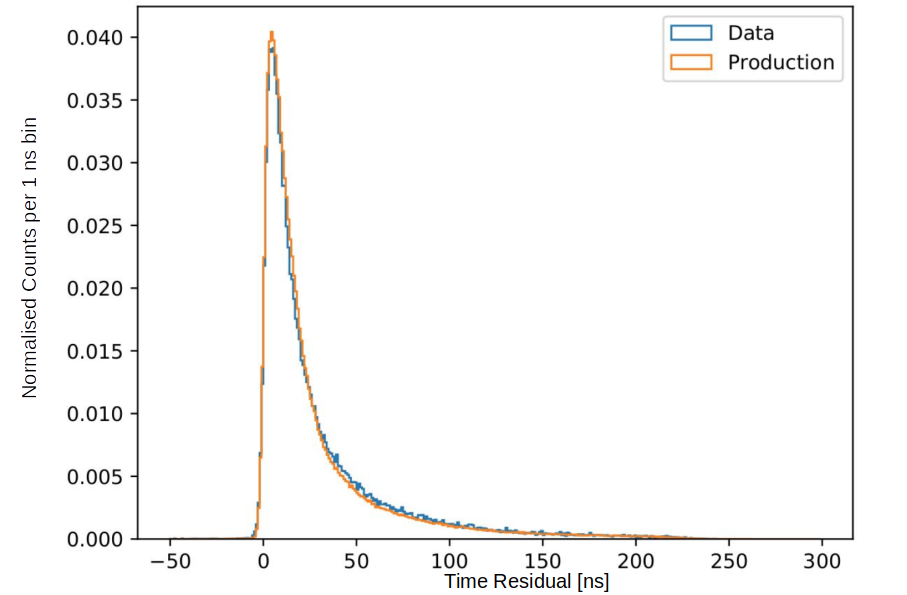
\includegraphics[width=0.8\linewidth]{2_Detector/Figs/scintillator_timing_data_mc.png}
    \caption[]{Comparison between the observed emission time distribution of electrons from tagged \ce{^{214}Bi} $\beta$-decays and a production of matching simulated events, after fitting the timing constants. Taken from~\cite{hunt-stokesEmissionTimingTuning2022}.%
    }
    \label{fig:typical_tres_dist_physics}
\end{figure}

When using just a single scintillating compound, the very same energy levels that can generate scintillation light are those that can absorb it. This can be a problem for large-scale detectors like SNO+, which depend on scintillation light being unobstructed in its path to the PMTs. This problem can be addressed with the addition of another scintillating component, known (somewhat confusingly) as the primary fluor. In SNO+, this is the PPO added to the LAB.

When an LAB molecule is excited, that energy can be transferred to a PPO molecule through what is known as a `non-radiative transfer'. In short, this transfer of energy occurs not through the emission and absorption of optical photons, but through the coupling of the molecules' electric dipoles during a collision. When the now-excited PPO molecule de-excites to emit scintillation light, the different molecular structure it has generates a different emission spectrum to that of LAB. These longer wavelengths of light are no longer able to be absorbed by the LAB, allowing for a scintillator with less optical absorption.

In SNO+ we plan on also adding in the compound BisMSB to the scintillator cocktail. This is a `wavelength-shifter': scintillation light at short wavelengths is absorbed, and then re-emitted at longer wavelengths, where the detection efficiency of the PMTs is greatest ($\sim\SI{420}{\nm}$). More on the properties of the PMTs in SNO+ can be found in Section~\ref{sec:pmts}. The net effect of the three scintillating components within SNO+ can be seen in Fig.~\ref{fig:cherenkov_scintillator_abs_emit_dist}. Note how, as energy is transferred from one scintillation component to another, the wavelength of light emitted gets necessarily longer as energy is lost to heat.



The light yield of a scintillator, i.e. the amount of optical photons generated per unit of energy deposited into the scintillator, is a function not just of the scintillator but also the incident particle's ionisation strength. In particular, $\alpha$ particles are far more effective at exciting and ionising nearby atoms, and so can deposit far more of its energy into the scintillator per unit volume. However, the strength of this ionisation for $\alpha$s can actually become at detriment to the generation of scintillation light. Empirically, scintillators follow to first order Birks' Law for their scintillation light yield~\cite{birksChapterScintillationProcess1967a}: % Birks Law ref.
\begin{equation}
    \frac{dL}{dx} = S\frac{\frac{dE}{dx}}{1+k_{\mathrm{Birks}}\frac{dE}{dx}},
\end{equation}
where $\frac{dL}{dx}$ is the number of photons emitted per unit track length, $\frac{dE}{dx}$ is the energy loss of the incident particle per unit track length, $S$ is the scintillator's characteristic light yield constant, and $k_{\mathrm{Birks}}$ is the scintillator's ``Birks' Constant''. For minimum-ionising particles such as a \SI{6}{\MeV} electron $\frac{dE}{dx}\approx\SI{2}{\MeV\per\cm}$~\cite{}, % cite PDG?
meaning the denominator of this equation is close to 1, and so the amount of scintillation light generated is just $\frac{dL}{dx} \approx S\cdot\frac{dE}{dx}$. However, for $\alpha$-particles generated in radioactive decays, this denominator can become substantial, and in the limiting case we have merely $\frac{dL}{dx} \approx \frac{S}{k_{\mathrm{Birks}}}$. For example, $\alpha$-particles are generated at \SI{5.304}{\MeV} from the decays of \ce{^{210}Po} nuclei~\cite{kondevNuclearDataSheets2008}. However, in the \SI{2.2}{\gpl} LABPPO scintillator currently within SNO+, we observe that these events generate light equivalent to a \SI{0.45}{\MeV} event. For this scintillator, $S$ and $k_{\mathrm{Birks}}$ are measured to be approximately \SI{14000}{\gamma\per\MeV} and \SI{0.077}{\mm\per\MeV}, respectively~\cite{riccettoRATOptics2g2022}. % cite where we got S and kb values from.


 \subsection{Optical Processes}\label{sec:optical_processes}
 Once optical-wavelength photons have been created within the detector, various processes can then occur that can hinder its path towards a PMT, and therefore modify the observed signal. This subsection covers the main optical processes, with a focus on Rayleigh scattering, as an understanding of this phenomenon is critical for Chapters~\ref{chap:smellie_hardware}--\ref{chap:smellie_analysis}.
 \subsubsection{Rayleigh Scattering}
Optical scattering is the general process of how light is scattered by particles within a medium. This is fundamentally an electrodynamical process: an electromagnetic wave is incident on the set of particles within the medium, which induces these particles to oscillate within the field, and therefore generating their own electromagnetic radiation in response. Usually, this `scattered' radiation has the same frequency as that of the incident radiation, and therefore the scattering is said to be \textit{elastic}. It is possible under certain circumstances for this scattered radiation to be of a longer wavelength than the incident radiation: in which case, energy was absorbed by the particles and so the scattering was \textit{inelastic}. However, this latter type of scattering, also known as Raman scattering, is not relevant for SNO+.

The general solution to elastic optical scattering was first described by Gustav Mie~\cite{mieContributionsOpticsTurbid1908} % ref Mie theory paper
and Ludvig Lorenz~\cite{lorenzLumiereReflechieRefractee1898} % Lorenz's paper
in what is now known as \textit{Mie Theory}. In this theory, it is assumed that a plane wave of wavelength $\lambda$ is incident on a dielectric sphere of radius $a$. While the general solution to the problem of Mie scattering is somewhat complicated (if tractable), in certain regimes one can make further simplifying assumptions that substantially reduce the complexity of the result. In particular, if one assumes that the size of the particle is much smaller than the wavelength of light, and that any induced dipole moment can actually be established in the time window allowed by the oscillation period of the electromagnetic field~\cite{HulstH.C.vande1981Lsbs}, % Rayleigh criteria
then one can obtain \textit{Rayleigh scattering}. This simpler case is so-called because of its initial formulation by Lord Rayleigh~\cite{rayleighTransmissionLightAtmosphere1899}. % Rayleigh's scattering paper

One can show that the differential cross-section associated with Rayleigh scattering of unpolarised light off a single particle, $\frac{d^{2}\sigma_{\textrm{Ray}}}{d\theta d\phi}\left(\theta,\phi\right)$, is given by~\cite{jacksonSection10Scattering1998}: % cite something that gets rayleigh scattering formula
\begin{equation}
    \frac{d^{2}\sigma_{\textrm{Ray}}}{d\theta d\phi}\left(\theta,\phi\right) = \frac{8\pi a^{6}}{\lambda^{4}}\left(\frac{n_{\textrm{par}}^{2}-1}{n_{\textrm{par}}^{2}+2}\right)^{2} \left(1+\cos^{2}\theta\right).
\end{equation}
Here, $\theta$ and $\phi$ correspond respectively to the polar and azimuthal angles of the scattered waves relative to the incoming wave, and $n_{\mathrm{par}}$ is the refractive index of the scattering particle. Most important to notice about this equation is that the cross-section follows a strong $1/\lambda^{4}$ dependence, meaning that short wavelengths of light will be scattered to far greater extents than that of longer wavelengths. Secondly, the light is not scattered isotropically, but according to a $1+\cos^{2}\theta$ dependence. This means that most light is either scattered directly forwards or backwards, and little gets scattered orthogonally to the direction of the incident light. This is useful when it comes to trying to measure scattering in the SNO+ detector, as it provides a handle upon which to distinguish scattered light from isotropically-emitted scintillation light.

Of course, we care about the scattering that occurs within an entire bulk medium, not just the scattering off of a single molecule. From a macroscopic perspective, the key quantity of interest is a material's \textit{Rayleigh scattering length}, $l_{\textrm{Ray}}$: the mean distance a photon is expected to travel before Rayleigh scattering. One can show that, assuming the above differential scattering cross-section, the Rayleigh scattering length is given by~\cite{zhouRayleighScatteringLinear2015}: % https://arxiv.org/pdf/1504.00987.pdf
\begin{equation}
    l_{\textrm{Ray}} = \left[\frac{16\pi}{3}R\right]^{-1}.
\end{equation}
$R$ is the \textit{Rayleigh ratio}, $R=\frac{1}{V}\frac{d^{2}\sigma_{\textrm{Ray}}\left(\ang{90}\right)}{d\theta d\phi}$, where $V$ is the volume taken up by one scattering particle within the medium. $R$ is then equivalent to the power of the scattered light per unit volume of the scattering medium per unit incident intensity at $\theta=\ang{90}$.

This can lead to a few changes to Rayleigh scattering that are worth noting. Firstly, unlike for a single particle, the electric polarisability of a material can be \textit{anisotropic}. Anisotropic materials have a modified angular dependence on their differential cross-section, governed by the \textit{depolarisation ratio}, $\delta$. In particular, the $\left(1+\cos^{2}\theta\right)$ dependence becomes $\left(1+\frac{1-\delta}{1+\delta}\cos^{2}\theta\right)$. For isotropic materials, $\delta=0$, and so the angular dependence reduces to the original form.

Secondly, the above model has been shown to be insufficient to describe liquids or solids~\cite{JerlovNilsGunnar1974Oaoo}, % optical aspects of oceanography!
because of the non-negligible strength of their inter-molecular forces. Fortunately, Einstein~\cite{einsteinTheoryOpalescenceHomogeneous1910}, %
Smoluchowski~\cite{smoluchowskiMolecularKineticTheory1908}, %
and Cabannes~\cite{cabannesRelationshipDegreePolarisation1920} %
developed a theory for describing how photons can scatter off of the local charge density fluctuations that naturally are present in a medium because of the thermal motion of molecules. The theory shows that the Rayleigh ratio of a medium is related to the medium's dielectric constant, $\varepsilon$, by:
\begin{equation}
    R = \frac{\pi^{2}}{2\lambda^{4}}\left[\rho\left(\frac{\partial\varepsilon}{\partial\rho}\right)_{T}\right]^{2} k_{B}T \kappa_{T}\frac{6+6\delta}{6-7\delta},
\end{equation}
where $\rho$ is the density of the medium, $\left(\frac{\partial\varepsilon}{\partial\rho}\right)_{T}$ is the partial derivative of the dielectric constant with respect to a changing density assuming a constant temperature $T$, $k_{B}$ is the Boltzmann Constant, and $\kappa_{T}$ is the medium's isothermal compressibility. This latter quantity is given by the rate of change of volume given a changing pressure of the medium, all at a constant temperature.

Furthermore, the Eykman Equation~\cite{eykmanRecherchesRefractometriquesSuite1895,zhouRayleighScatteringLinear2015} % I LIKE EYK!
has been shown to be an effective empirical formula relating how $\varepsilon$ is impacted by density fluctuations to the medium's refractive index, $n_{\textrm{med}}$:
\begin{equation}
    \rho\left(\frac{\partial\varepsilon}{\partial\rho}\right)_{T} = 
    \frac{\left(n_{\textrm{med}}^{2}-1\right)\left(2n_{\textrm{med}}^{2}+0.8n_{\textrm{med}}\right)}{n_{\textrm{med}}^{2}+0.8n_{\textrm{med}}+1}.
\end{equation}
This leads to a final empirical formula for the Rayleigh scattering length:
\begin{equation}
    l_{\mathrm{Ray}} = \left[
        \frac{8\pi^{3}}{3\lambda^{4}}
        \left(
            \frac{\left(n_{\textrm{med}}^{2}-1\right)\left(2n_{\textrm{med}}^{2}+0.8n_{\textrm{med}}\right)}{n_{\textrm{med}}^{2}+0.8n_{\textrm{med}}+1}
        \right)^2
        k_{B}T \kappa_{T}\frac{6+3\delta}{6-7\delta}
        \right]^{-1}.
\end{equation}

In-situ measurements of the scattering of the UPW were made indirectly during SNO~\cite{moffatOpticalCalibrationSudbury2001}, and then subsequently in the water phase of SNO+ had a divisive scaling factor of $(1.28\pm0.05(\mathrm{stat.})\pm0.14(\mathrm{sys.}))$ determined by Esther Turner~\cite{turnerMeasurementScatteringCharacteristics2022}. Ex-situ measurements of the Rayleigh scattering within LAB and LABPPO have also been made by groups in both the SNO+ and JUNO Collaborations~\cite{chenOpticalPropertiesRAT2012,seguiScintillatorModelComparison2015,liuAttenuationScatteringTeBD2016,liuRayleighScatteringDepolarization2015,yuMeasurementsRayleighRatios2022}, %
but no in-situ measurements have been made prior to this thesis. Fig.~\ref{fig:scattering_lengths_upw_labppo_current} shows the scattering lengths for UPW, LAB, and \SI{2}{\gpl} LABPPO from these measurements, with the lines showing what is currently being used in simulations for SNO+. Measurements of the scattering lengths in scintillator are a major focus of Chapters~\ref{chap:smellie_hardware}--\ref{chap:smellie_analysis}.

\begin{figure}[!ht]
    \centering
    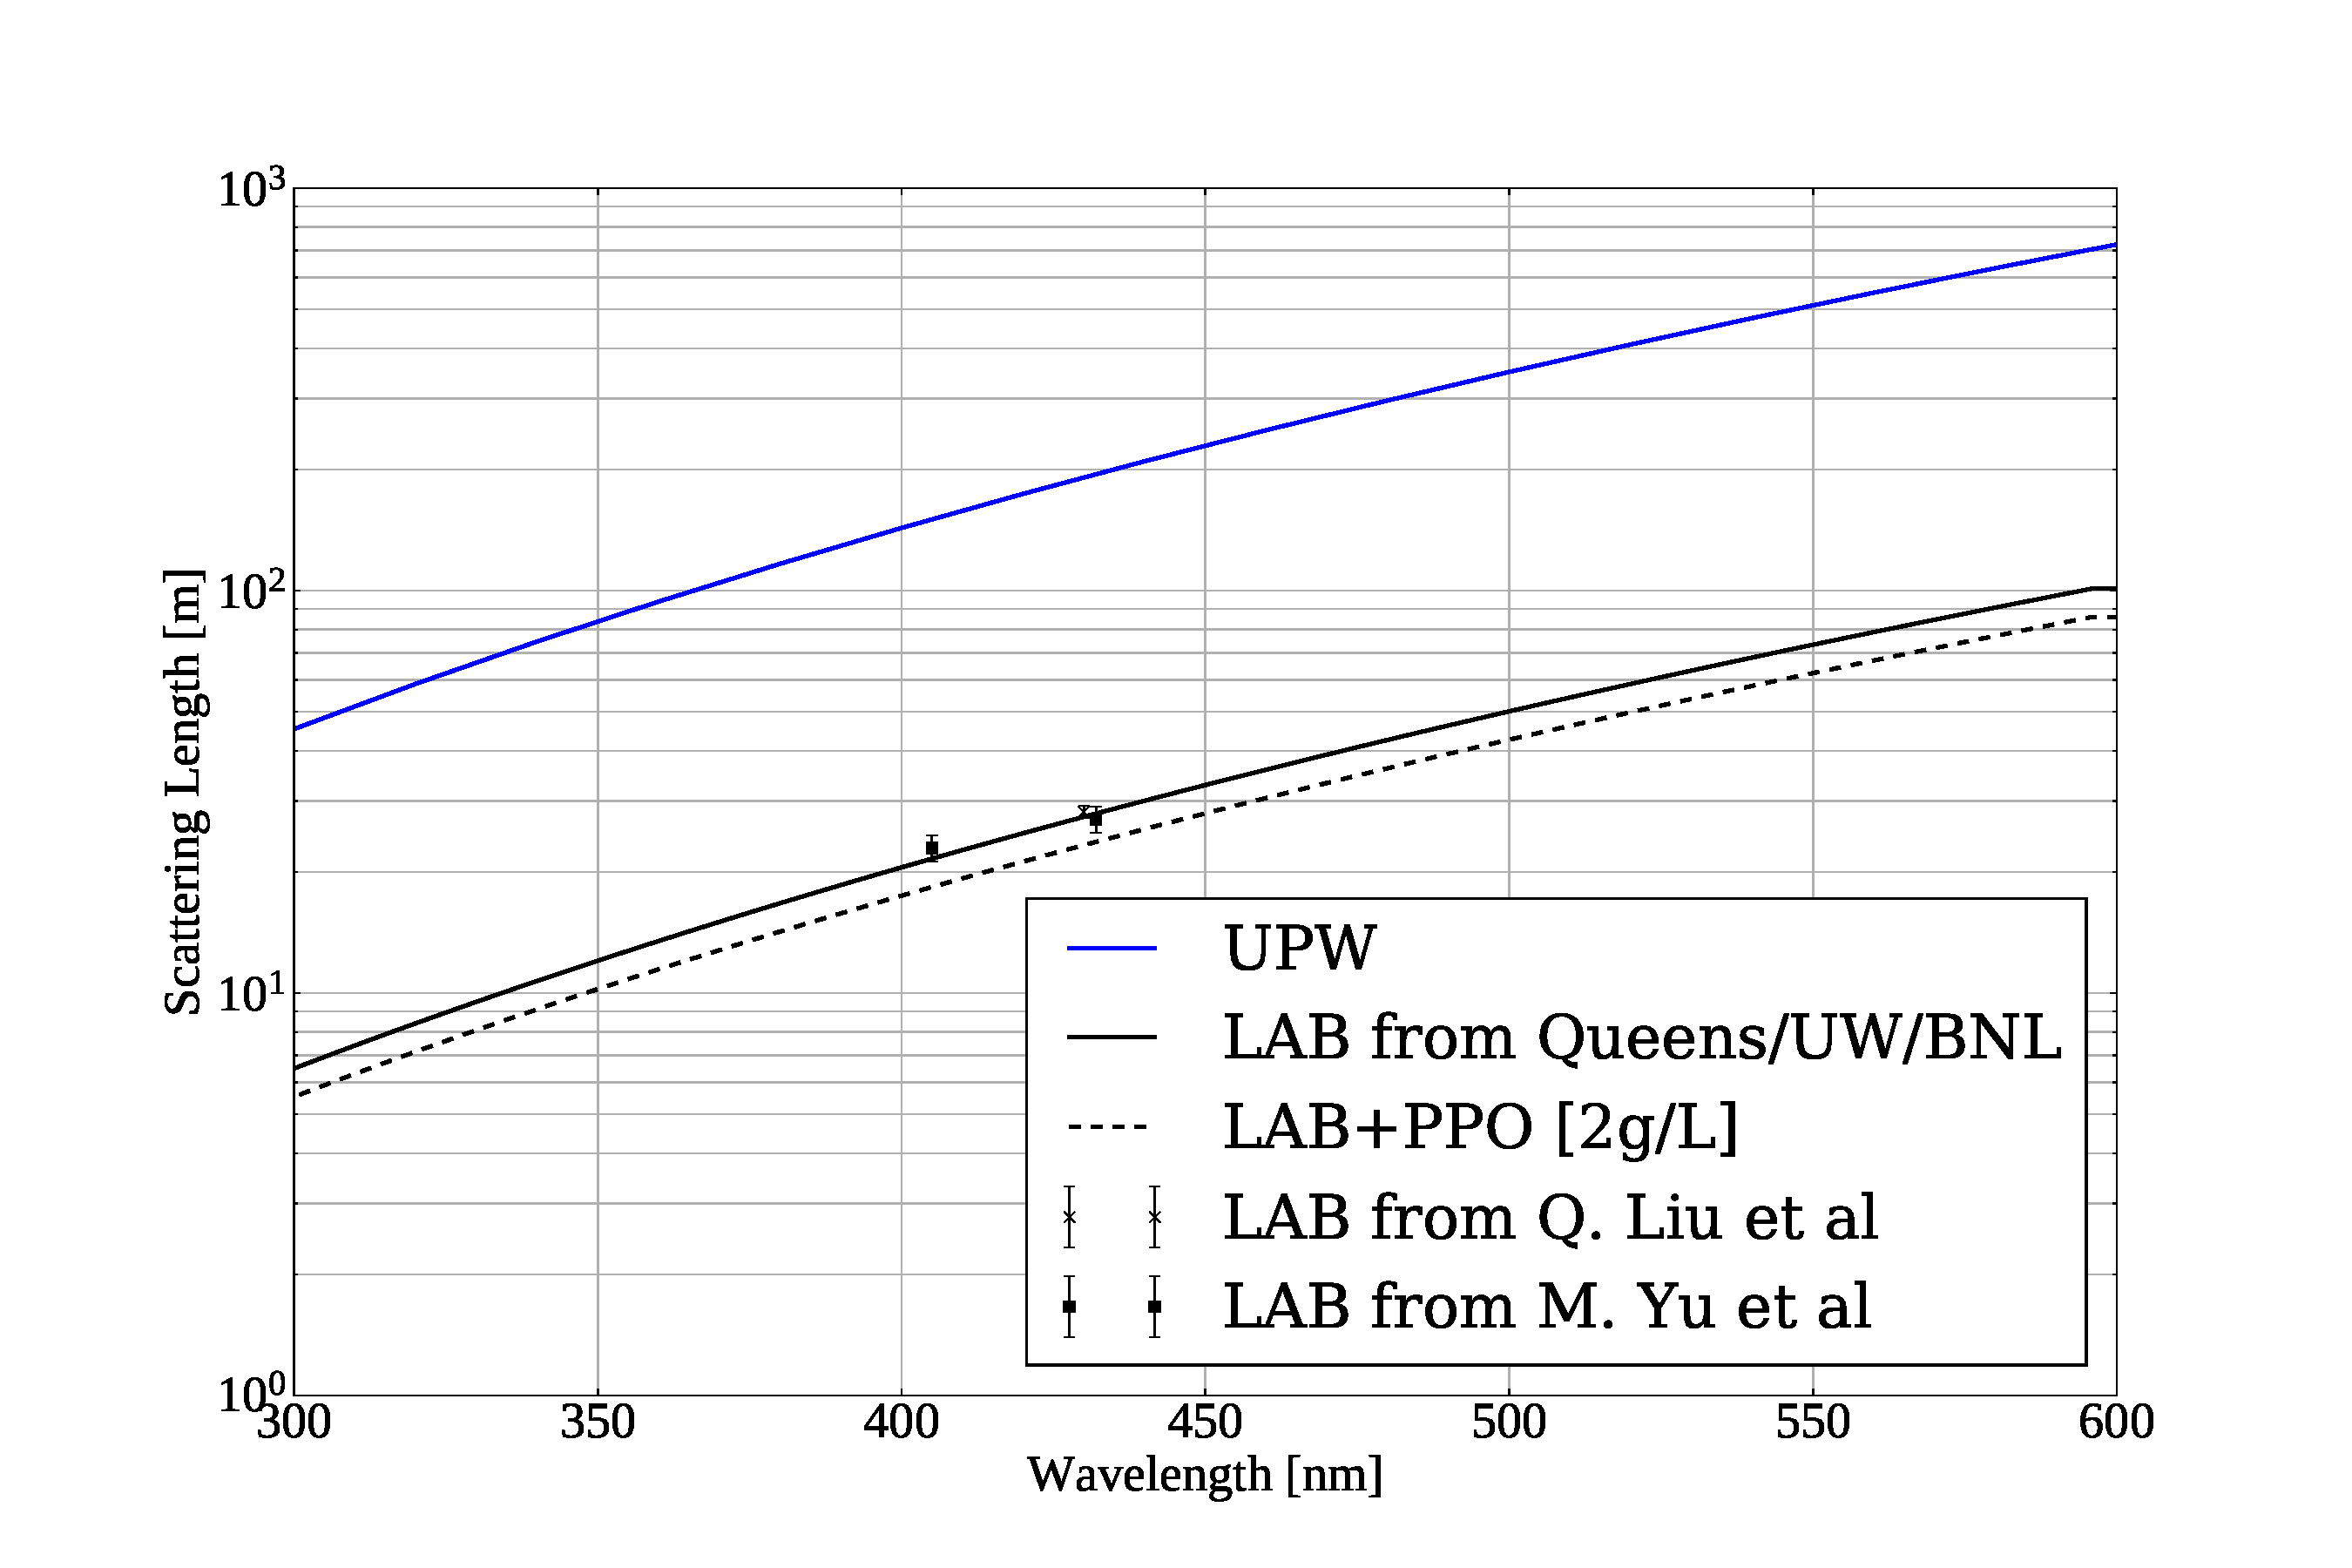
\includegraphics[width=0.8\linewidth]{2_Detector/Figs/scattering_lengths_plot.pdf}
    \caption[Scattering lengths in simulation for UPW, LAB, and \SI{2.2}{\gpl} LABPPO]
    {Scattering lengths used in simulation for UPW, LAB, and \SI{2}{\gpl} LABPPO. The UPW shape is taken from indirect in-situ measurements in~\cite{moffatOpticalCalibrationSudbury2001} with an additional divisive scaling factor from~\cite{turnerMeasurementScatteringCharacteristics2022}. The LAB shape is taken from ex-situ measurements by SNO+ members at Queen's University, University of Washington, and Brookhaven National Laboratory~\cite{chenOpticalPropertiesRAT2012,seguiScintillatorModelComparison2015}. An additional divisive scaling factor of 1.176 due to PPO was made by~\cite{liuAttenuationScatteringTeBD2016}. For comparison, measurements by members of the JUNO Collaboration for LAB are also shown~\cite{liuRayleighScatteringDepolarization2015,yuMeasurementsRayleighRatios2022}.}
    \label{fig:scattering_lengths_upw_labppo_current}
\end{figure}

    % \begin{itemize}
    %     \item Explain the electrodynamical model for scattering, giving rise to the expected $1/\lambda^4$ wavelength-dependence of the scattering length, as well as the $1+\cos^2\theta$ dependence of the scattering angle.
    %     \item Describe how the density-fluctuation theory gives rise to a possible modification to the scattering angle distribution due to the anisotropy of the optical media's polarisability vector. Studies by JUNO have shown that LABPPO has such a measurable anisotropy.
    %     \item Show the existing model for water and LABPPO used in RAT, and note that this anisotropy is currently not included in any simulations. I don't need to go in too much detail for this subsection as Krish did a nice job in his thesis and I can cite that, but I do need to write enough to cover the basics for my SMELLIE analysis chapter.
    % \end{itemize}
    % [3 pages]

\subsubsection{Absorption and Re-emission}
In addition to scattering, an optical medium is also able to absorb light that propagates through it. For a given medium, the \textit{absorption length} $l_{\mathrm{abs}}$ is analogous to $l_{\mathrm{Ray}}$ described above, and is typically strongly a function of wavelength. For most materials, absorbed light is forever lost, converted into heat. However, for the special case of scintillators, re-emission of absorbed light is possible: this is because of the physics described in Section~\ref{sec:scintillation}.

Because both scattering and absorption impede a photon's ability to propagate through a medium directly, it is often possible to measure their combined impact through what is known as the attenuation/extinction length, $l_{\mathrm{ext}}$:
\begin{equation}\label{eq:ext_length_def}
    \frac{1}{l_{\mathrm{ext}}} = \frac{1}{l_{\mathrm{abs}}} + \frac{1}{l_{\mathrm{Ray}}}.
\end{equation}
In the water phase, the `Laserball' calibration system was used by Ana Sofia In\'{a}cio to measure various optical properties of the detector, including the extinction lengths of the UPW and acrylic as a function of wavelength~\cite{andersonOpticalCalibrationSNO2021,inacioDataAnalysisWater2022}. Using the water phase scattering measurements made by E. Turner, Eq.~\ref{eq:ext_length_def} allowed for the estimation of the absorption lengths of these two materials, shown in Figure~\ref{fig:abs_lengths_optics_paper}. Measurements of the extinction length in the scintillator phase is discussed in detail in Chapter~\ref{chap:smellie_analysis}.

\begin{figure}
    \centering
    \begin{subfigure}{0.98\textwidth}
        \centering
        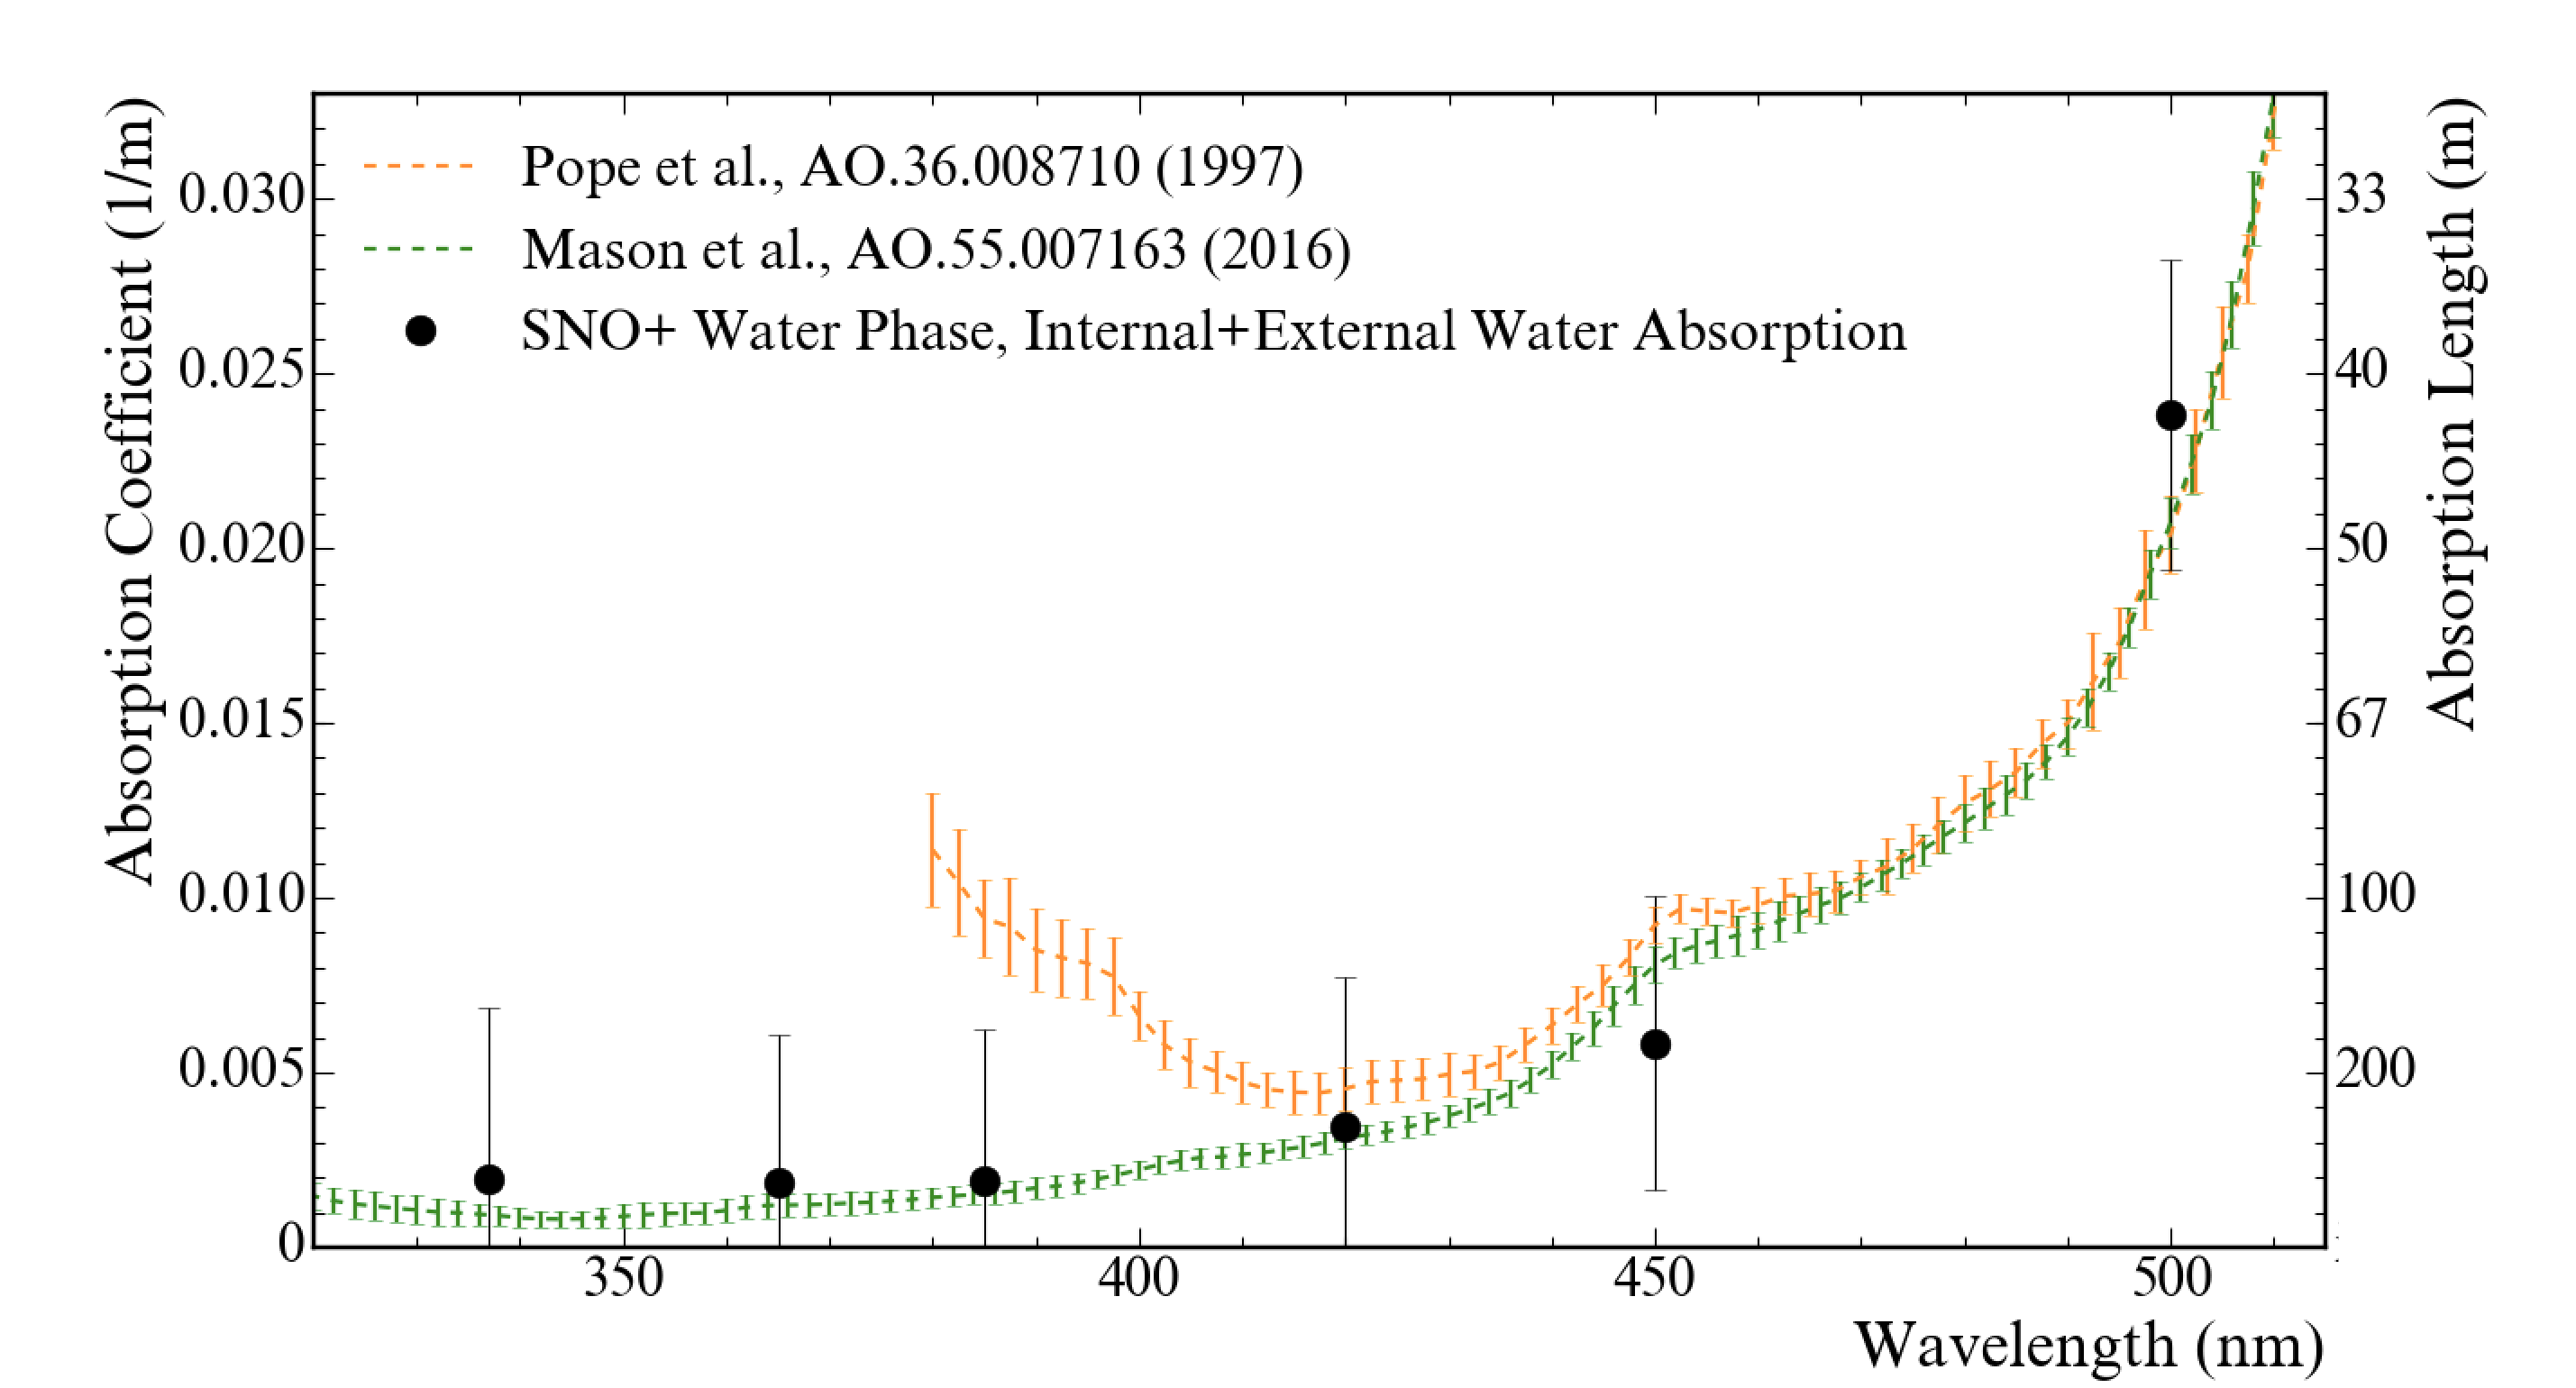
\includegraphics[width=0.9\textwidth]{2_Detector/Figs/WaterAbsorption.png}
        \caption{UPW optical absorption}
        \label{fig:abs_length_water_optics_paper}
    \end{subfigure}
    \begin{subfigure}{0.98\textwidth}
        \centering
        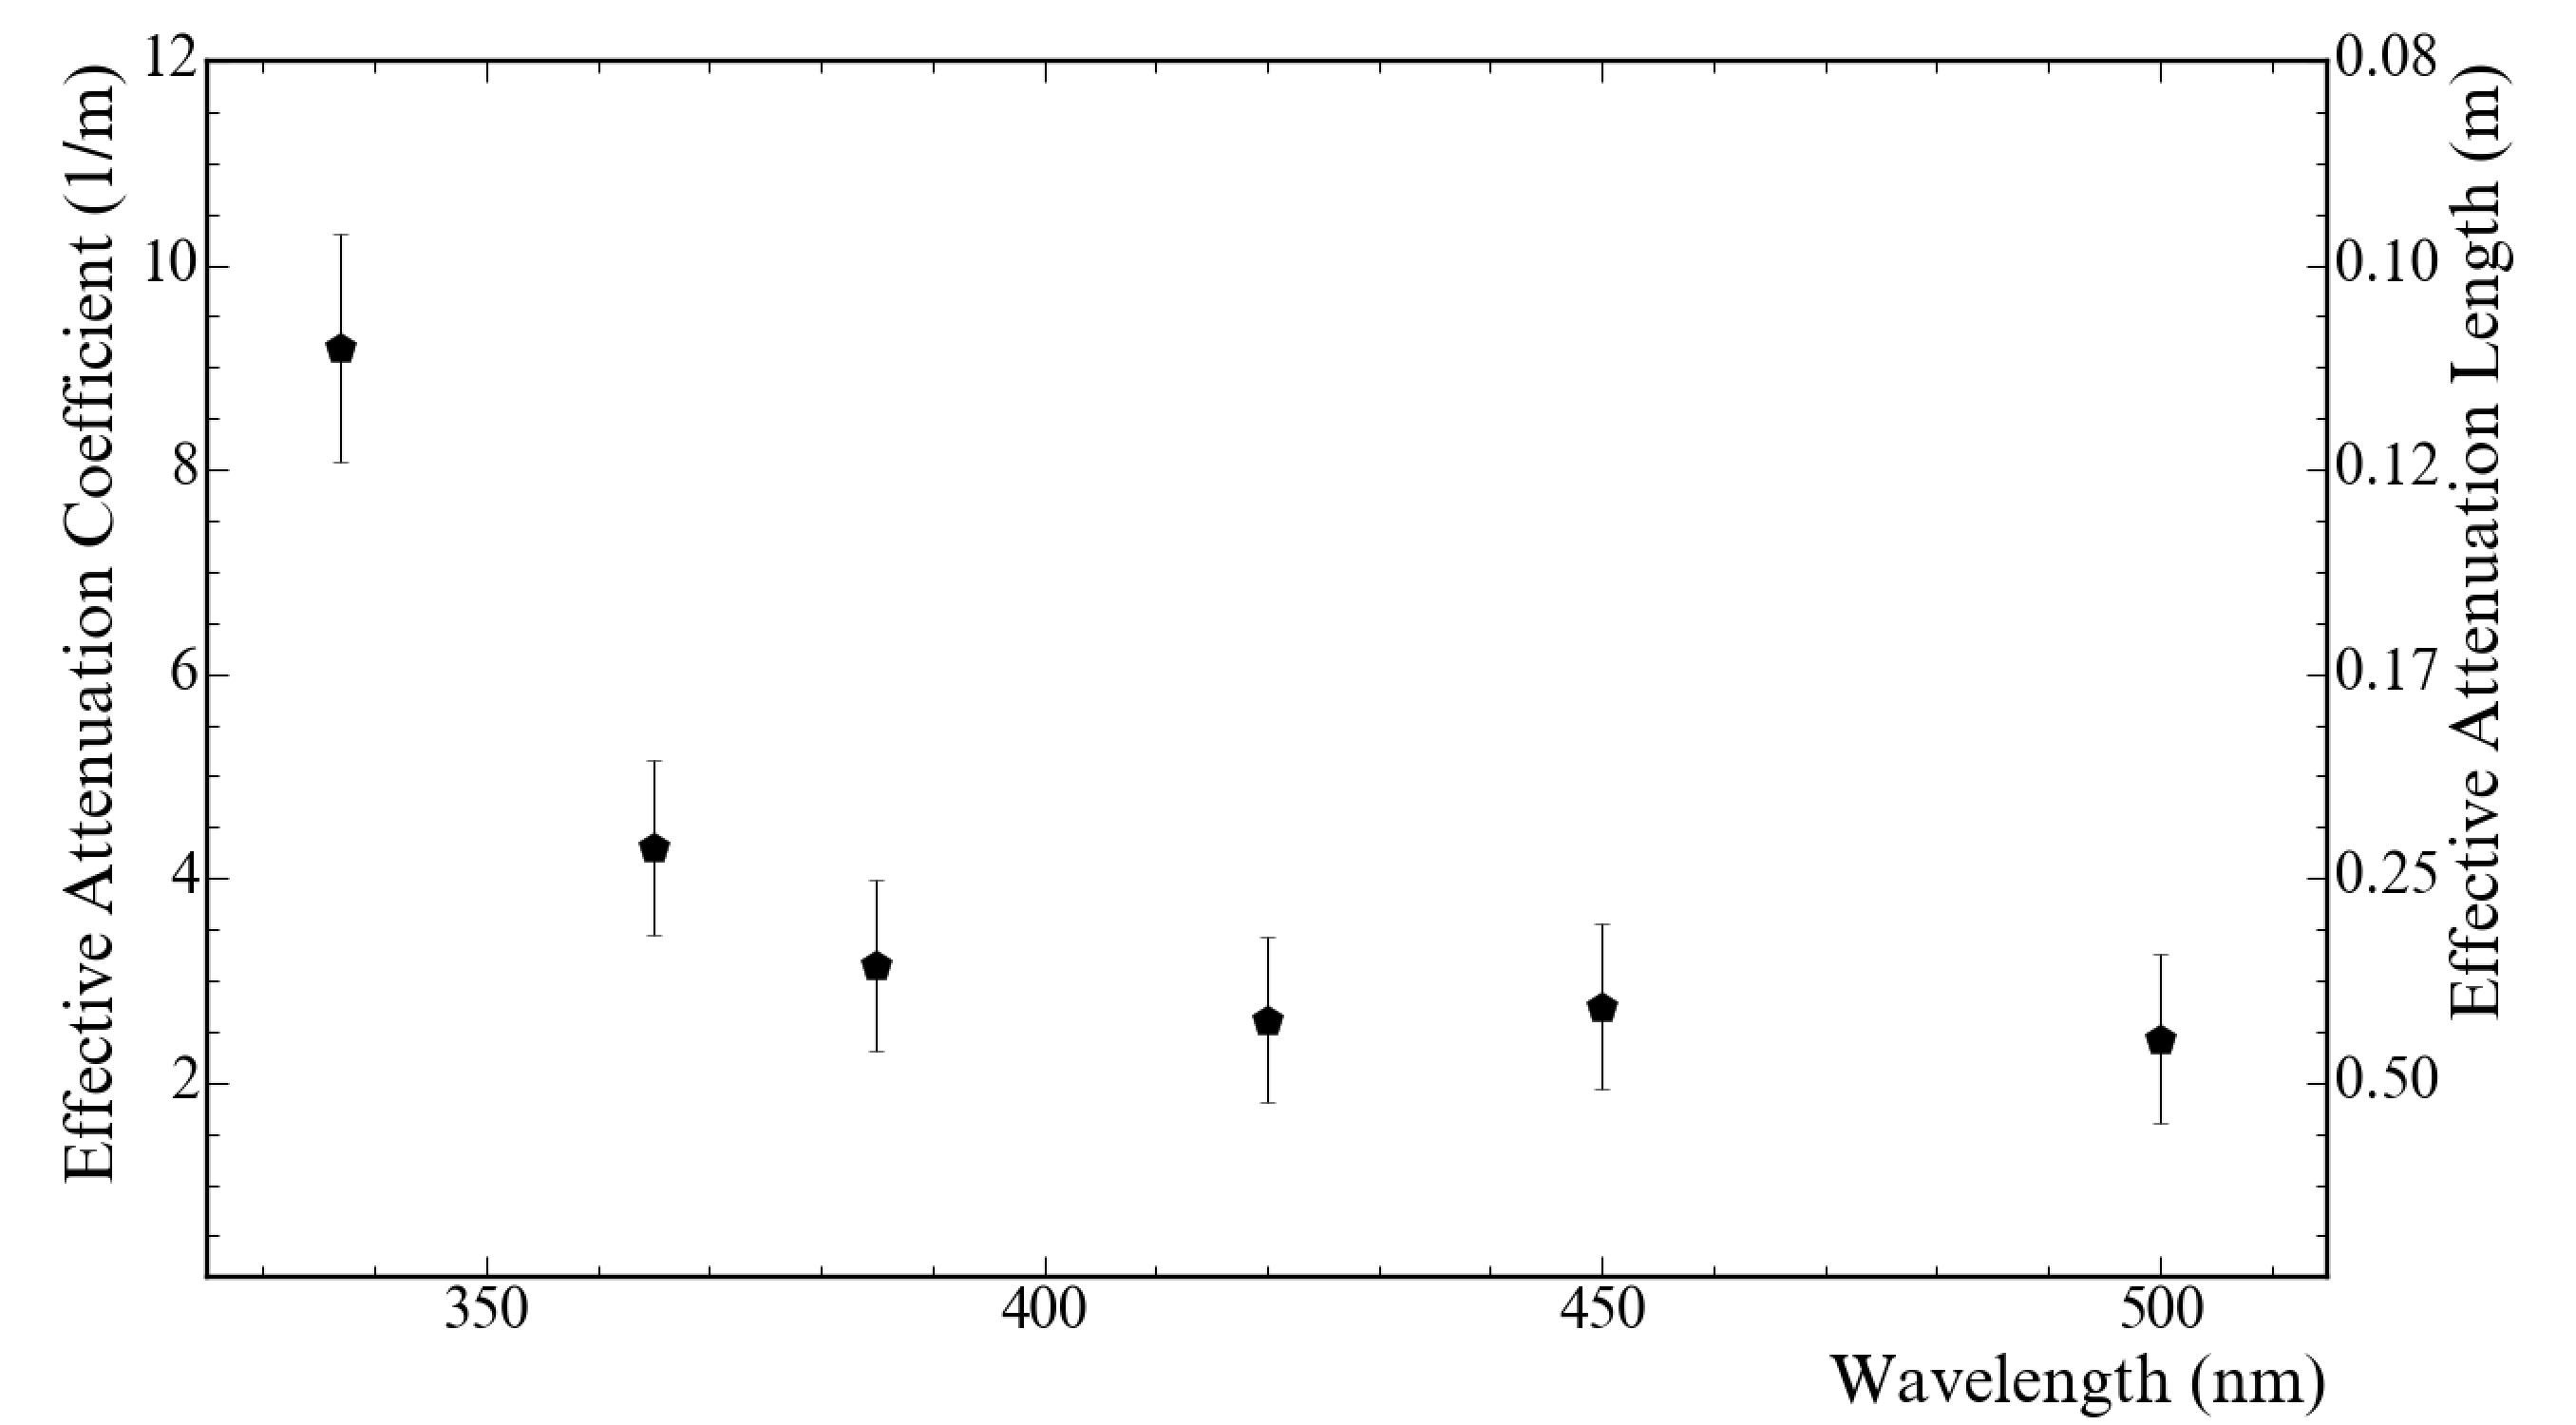
\includegraphics[width=0.85\textwidth]{2_Detector/Figs/AcrylicAttenuation.png}
        \caption{Acrylic optical attenuation}
        \label{fig:abs_length_acylic_optics_paper}
    \end{subfigure}
    \caption[Measured properties of the UPW and acrylic in the water phase.]
    {Properties of the UPW and acrylic in the water phase, measured by A. S. In\'{a}cio in~\cite{andersonOpticalCalibrationSNO2021,inacioDataAnalysisWater2022}.}
    \label{fig:abs_lengths_optics_paper}
\end{figure}

    % \begin{itemize}
    %     \item State that light can get absorbed by materials, and if that medium is a scintillator then re-emission is possible. I think further details such as the specific shape of the absorption/re-emission of the scintillator and water can be shown in the SMELLIE analysis chapter, in which I have to explain about possible changes to the model anyway.
    % \end{itemize}
    % [1/2 page]
\subsubsection{Surface reflection and refraction}
\nomenclature{\textbf{TIR}}{Total Internal Reflection}
When light travels through the boundary of one medium to another, both reflection and refraction can be possible, depending on the relative refractive indices of the two media as well as the angle of incidence. The refractive indices of the UPW, acrylic, and LABPPO are shown as a function of wavelength in Figure~\ref{fig:ref_indices_snoplus}. Note that, for most optical wavelengths, LABPPO has a very close refractive index to acrylic, whereas UPW is somewhat farther away. By consequence, negligible refraction is expected in most cases for light travelling between the liquid scintillator and the acrylic; however, substantial refraction and reflection are possible for light travelling between acrylic and UPW. Because of this, isotropically-emitting point-like physics events within the AV that are close enough to the acrylic will have some of their light undergo Total Internal Reflection (TIR) at the AV, reflecting back into the AV instead of continuing outward into the outer water.

% \begin{figure}
%     \centering
%     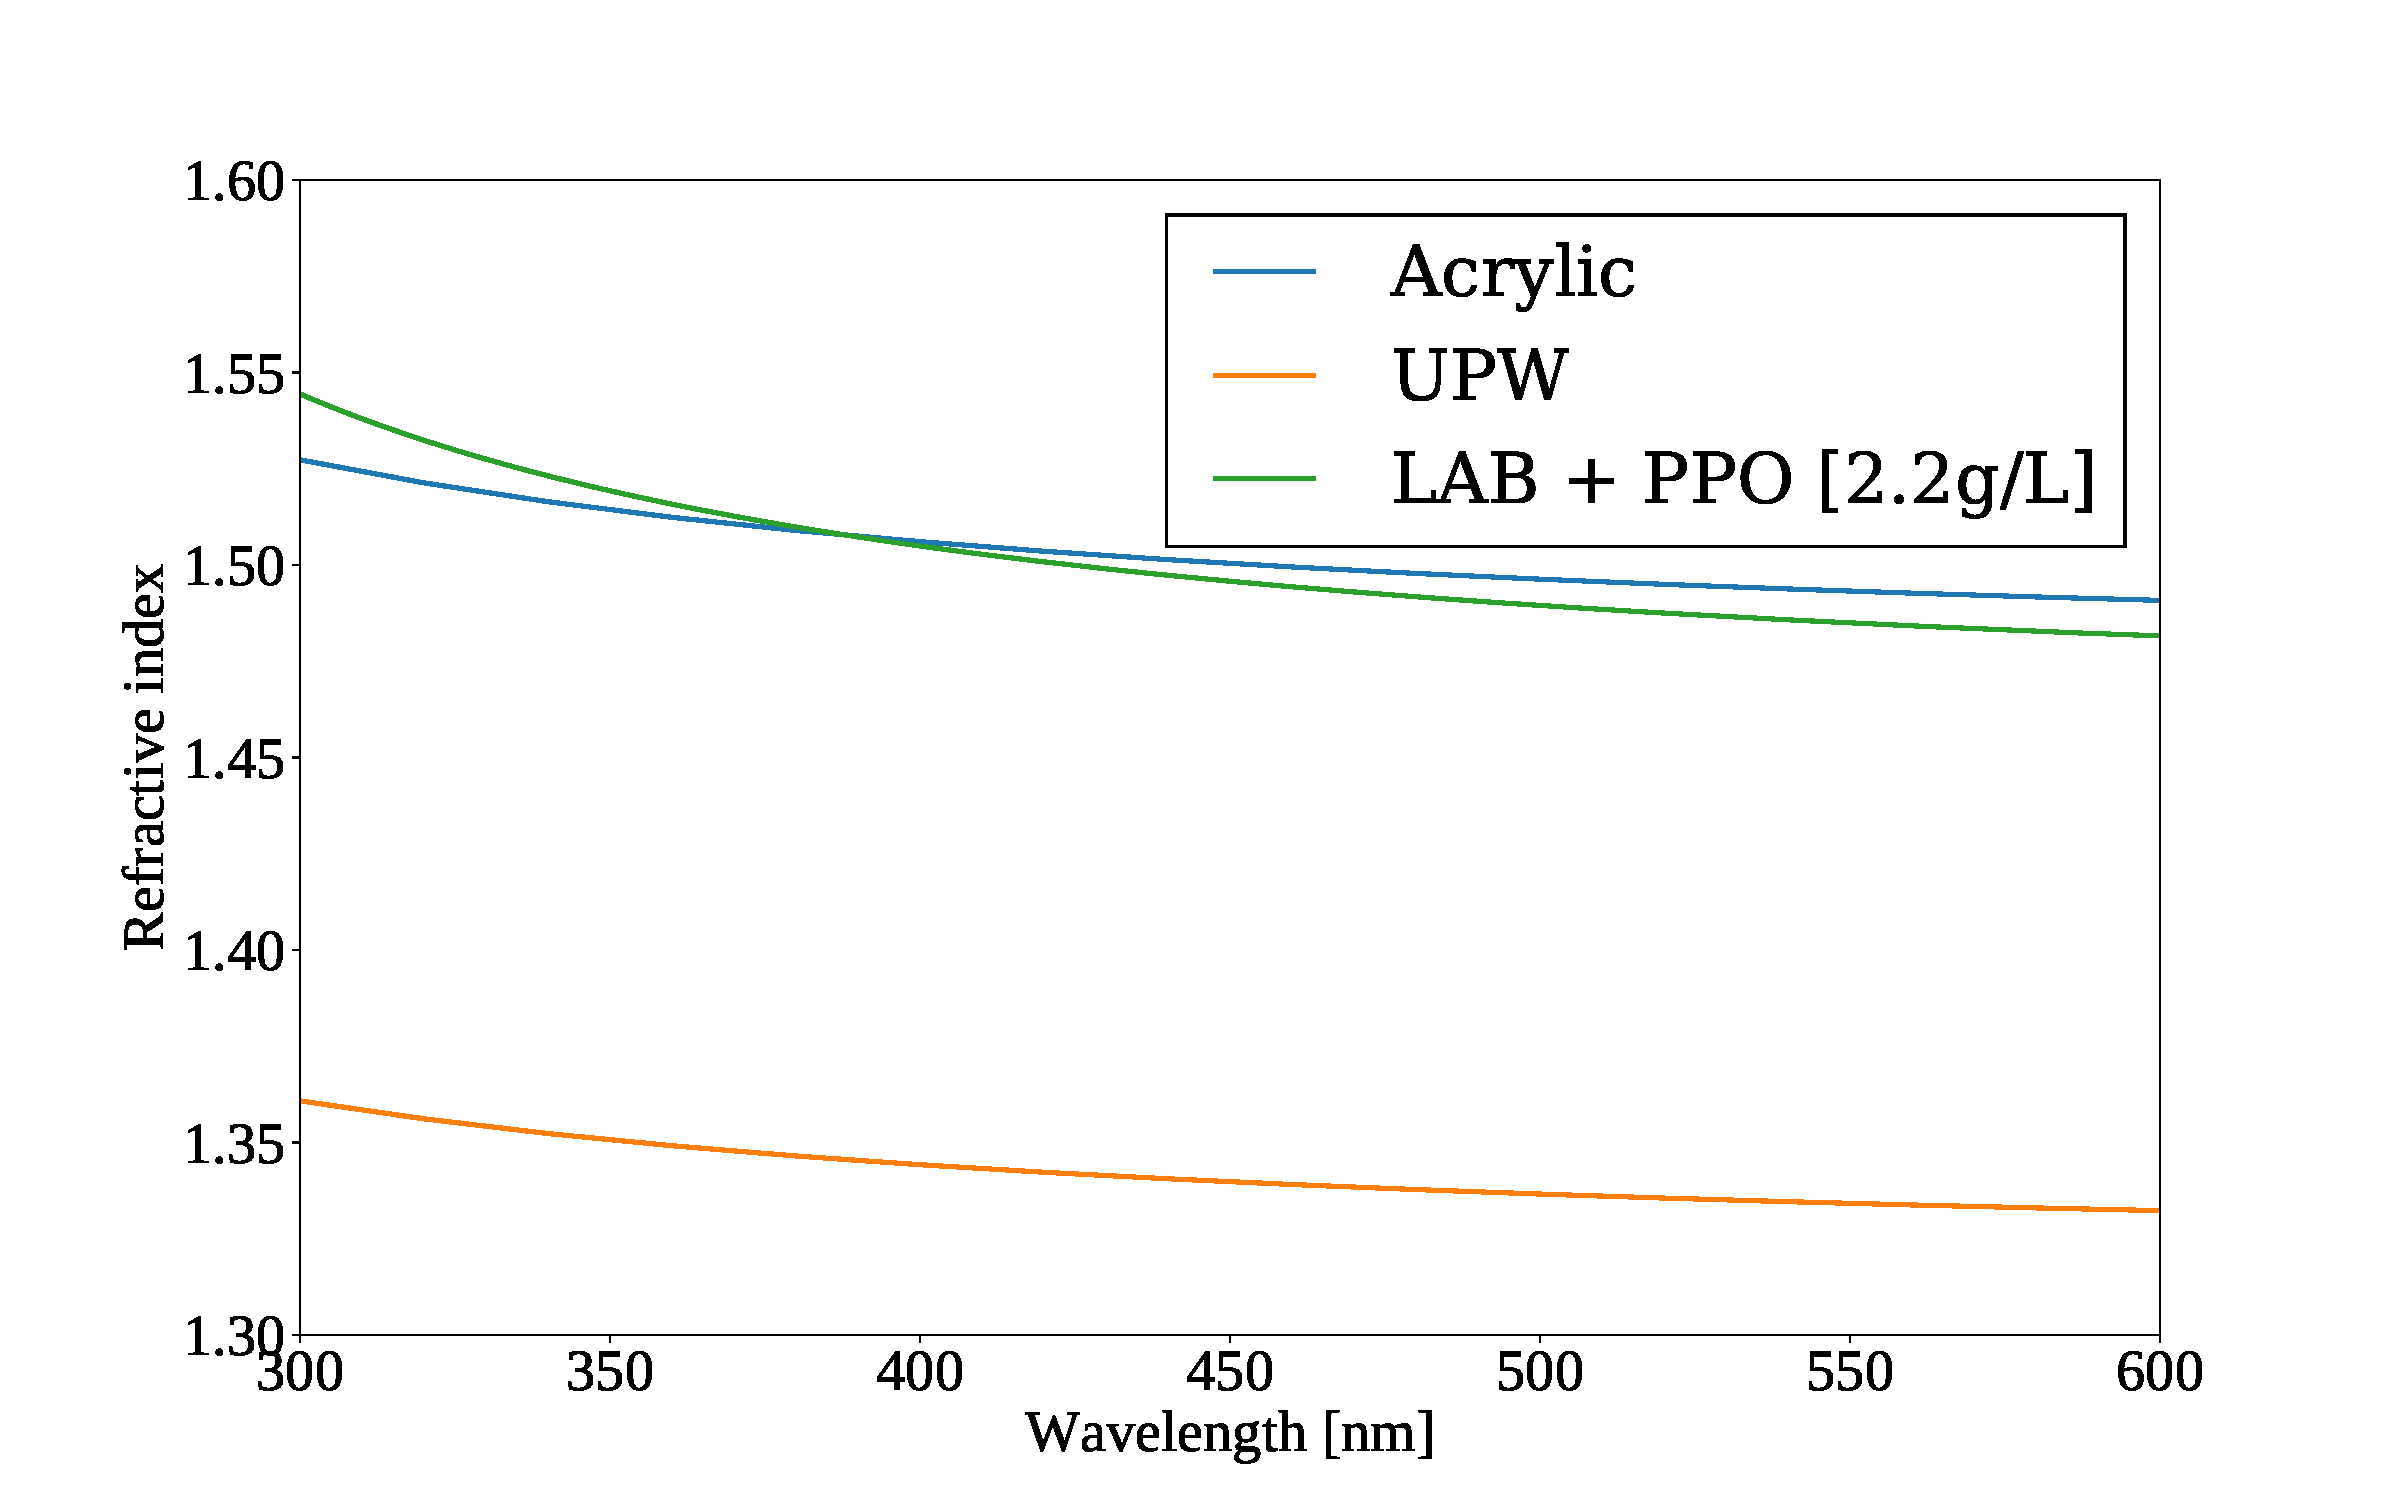
\includegraphics[width=0.8\linewidth]{2_Detector/Figs/refractive_indices_plot.pdf}
%     \caption[Refractive indices of acrylic, UPW, and LABPPO as a function of wavelength]
%     {Refractive indices of acrylic, UPW, and LABPPO as a function of wavelength~\cite{andersonOpticalCalibrationSNO2021,tseungEllipsometricMeasurementsRefractive2011,moffatOpticalCalibrationSudbury2001}. % cite!
%     }
%     \label{fig:ref_indices_snoplus}
% \end{figure}

\begin{figure}
    \centering
    \begin{subfigure}{0.48\textwidth}
        \centering
        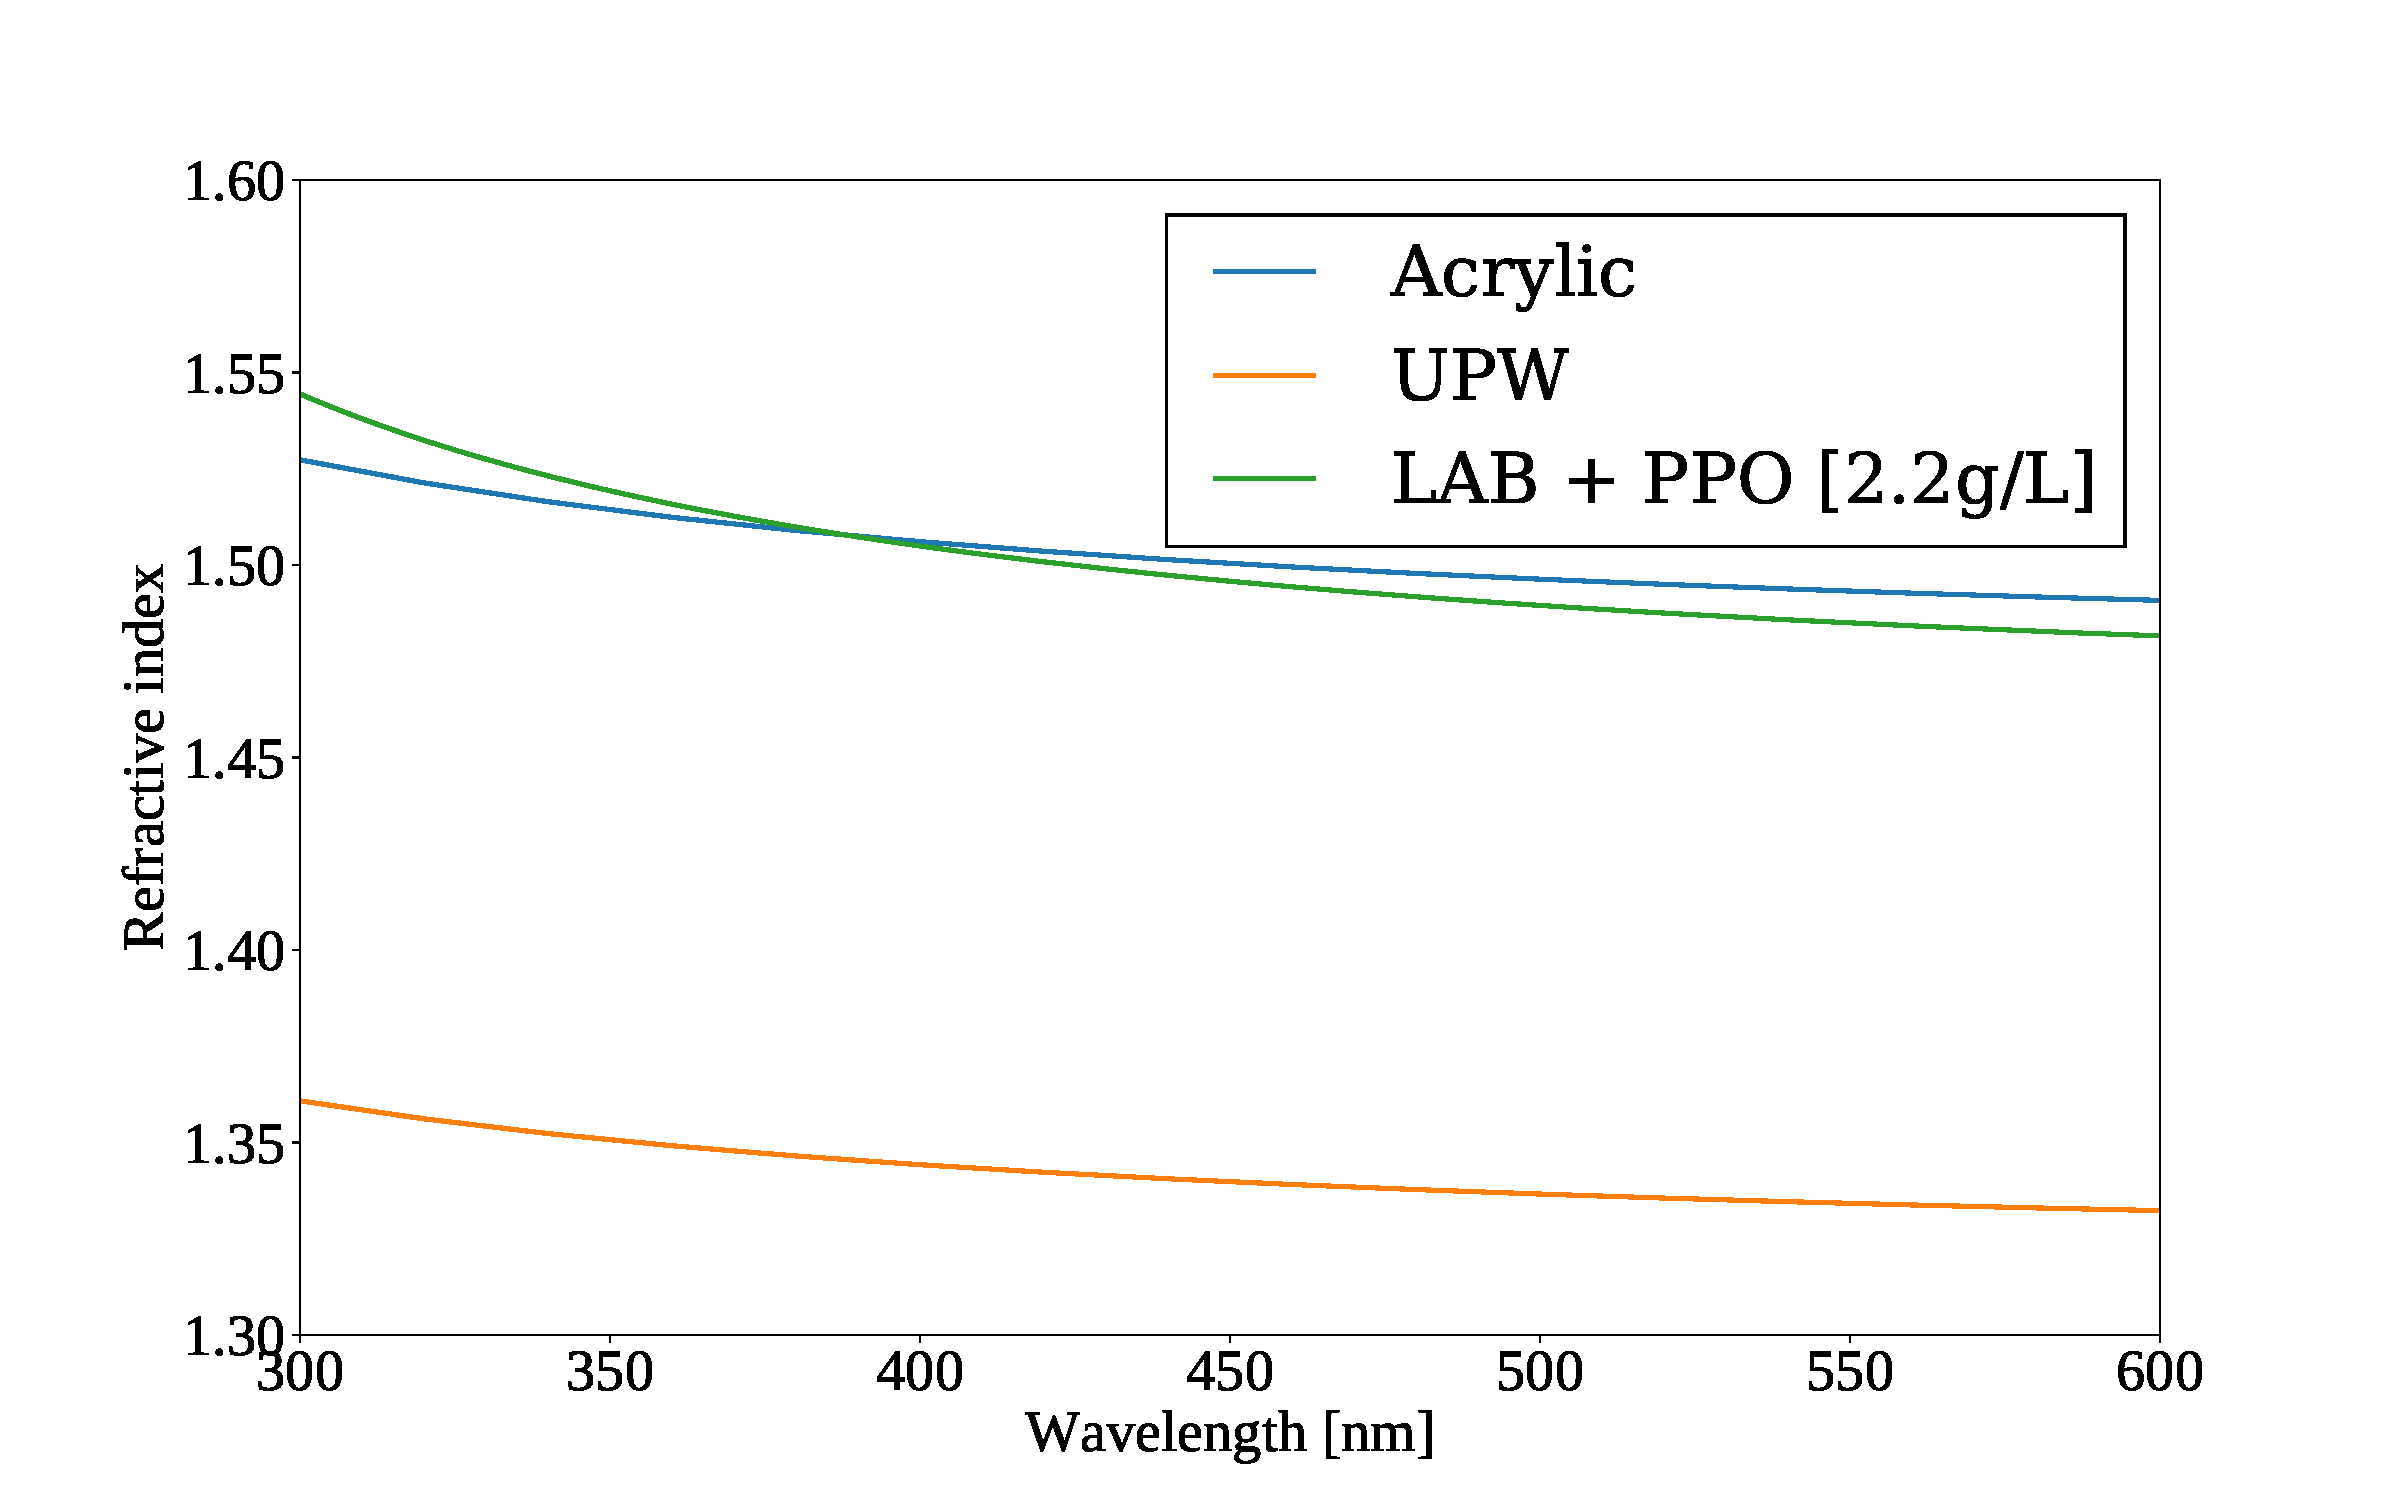
\includegraphics[width=0.95\linewidth]{2_Detector/Figs/refractive_indices_plot.pdf}
        \caption{}
        \label{fig:ref_indices_snoplus}
    \end{subfigure}
    \begin{subfigure}{0.48\textwidth}
        \centering
        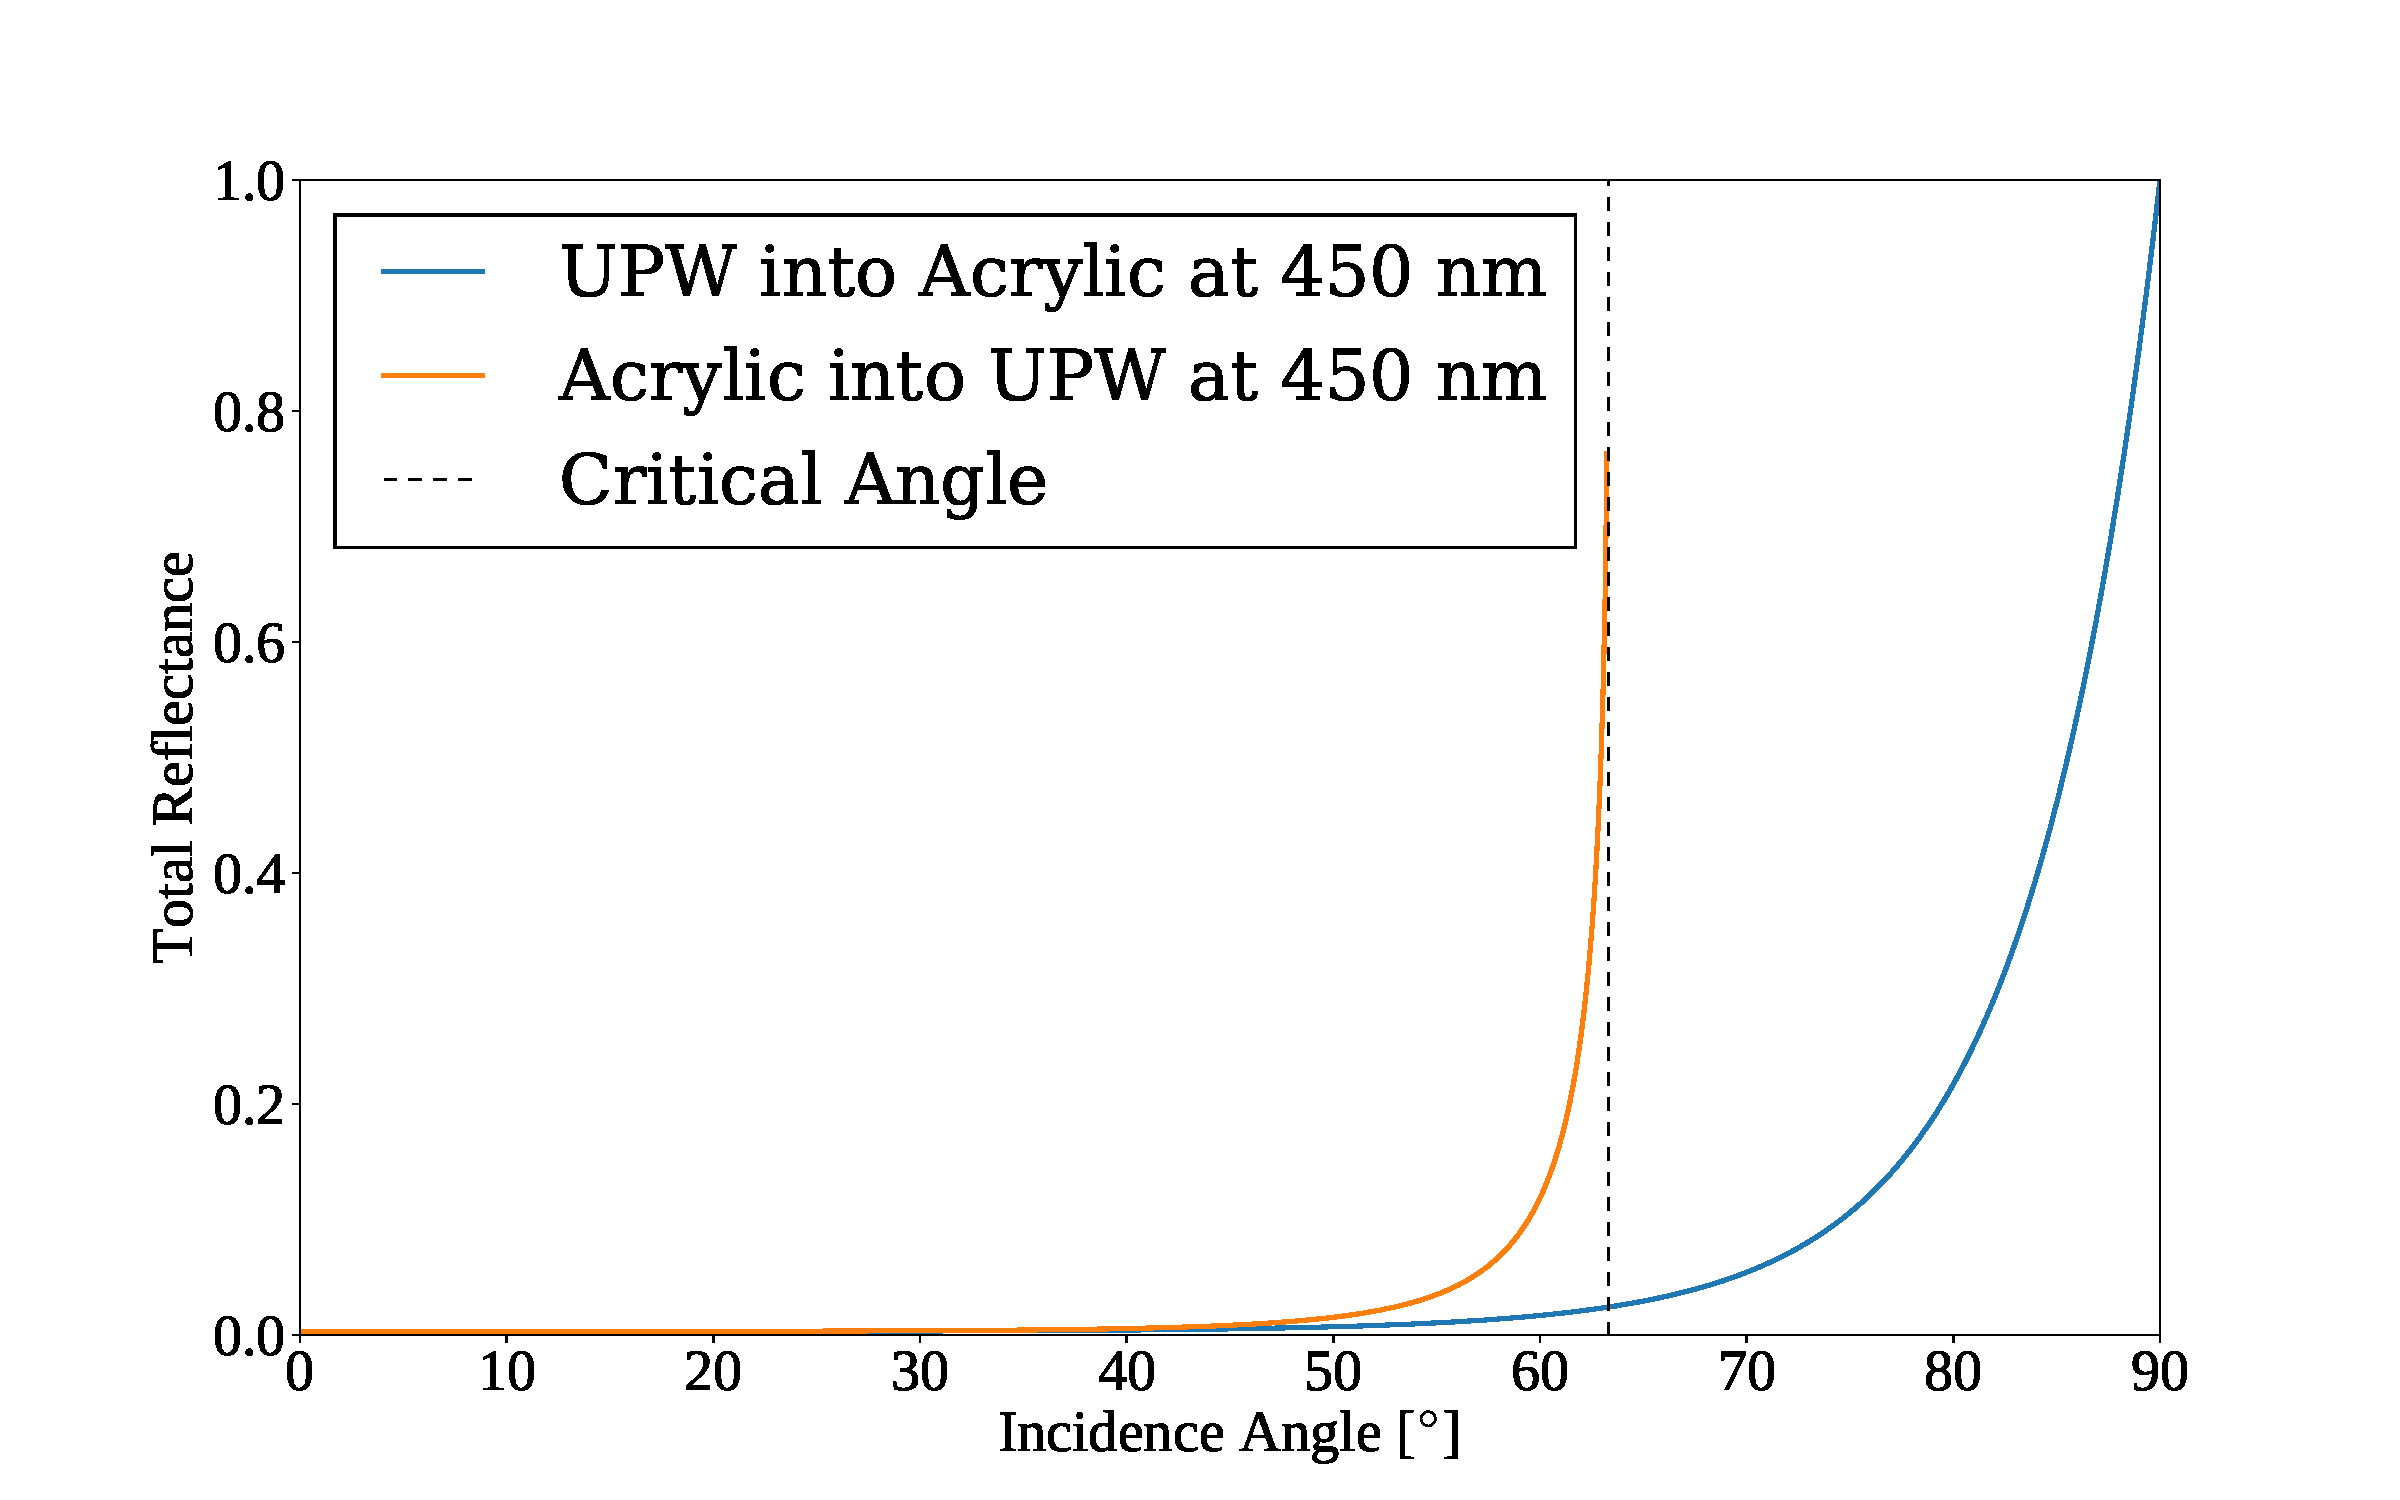
\includegraphics[width=0.95\linewidth]{2_Detector/Figs/reflectance_vs_angle_plot.pdf}
        \caption{}
        \label{fig:reflectance_vs_angle}
    \end{subfigure}
    \caption[Refractive indices of acrylic, UPW, and LABPPO as a function of wavelength; also reflectance as a function of incidence angle]
    {\textbf{(a):} Refractive indices of acrylic, UPW, and LABPPO as a function of wavelength. The values for acrylic and UPW come from model fits to data made in SNO~\cite{boardmanDetectionCherenkovRadiation1992,moffatOpticalCalibrationSudbury2001}, whereas those for LABPPO come from data taken in~\cite{tseungEllipsometricMeasurementsRefractive2011}. \textbf{(b):} Reflectance of an unpolarised beam of light at \SI{450}{\nm} going between UPW and acrylic.
    }
    \label{fig:ref_index_and_reflectance}
\end{figure}

Even when not undergoing TIR, some light at a boundary will still reflect. The fraction of light that reflects is known as the \textit{reflectance} $R$, compared to that which is able to transmit through the boundary, the \textit{transmittance} $T=1-R$. The \textit{Fresnel Equations} determine the reflectance of an interface~\cite{hechtSectionFresnelEquations2014}:% Fresnel eqs: Hecht?
\begin{equation}
    R_{s} = \left|\frac{n_{1}\cos{\theta_{i}}-n_{2}\cos{\theta_{t}}}{n_{1}\cos{\theta_{i}}+n_{2}\cos{\theta_{t}}}\right|^{2},\\
    R_{p} = \left|\frac{n_{1}\cos{\theta_{t}}-n_{2}\cos{\theta_{i}}}{n_{1}\cos{\theta_{t}}+n_{2}\cos{\theta_{i}}}\right|^{2},
\end{equation}
where $R_{s}$ and $R_{p}$ are the reflectances of $s$- and $p$-polarised light, $n_{1}$ and $n_{2}$ are the refractive indices of the first and second optical media, and $\theta_{i}$ and $\theta_{t}$ are the angles of incidence and refraction, respectively. For SNO+, we are only interested in unpolarised light, so the total reflectance $R = \left(R_{s}+R_{p}\right)/2$.

The total reflectance going from UPW into acrylic, as well as from acrylic into UPW, for an unpolarised beam of light with wavelength \SI{450}{\nm} is shown in Fig.~\ref{fig:reflectance_vs_angle}. For the latter case, the critical angle at which TIR occurs is clear.

    % \begin{itemize}
    %     \item State that boundaries between media can induce reflections and refraction, as governed by the Fresnel transmission and reflection formulae. These formulae are worth mentioning because I use them in my SMELLIE extinction length analysis.
    % \end{itemize}
    % [1/2 page]
\subsection{Detection by PMTs}\label{sec:pmts}
The final step for photons in our journey is detection by a PMT. Almost all PMTs in SNO+ are of the Hamamatsu R1408 design~\cite{BOGER2000172}. % cite
These PMTs within SNO+ are housed within an 18-segment reflecting Winston cone known as a `concentrator'. The combined PMT--concentrator `bucket', shown in Fig.~\ref{fig:pmt_conc_diagram}, is designed to maximise the collection efficiency of light emanating from within the AV, whilst minimising the collection efficiency of light outside the AV~\cite{moorheadReflectorsCherenkovDetectors1992}. % cite Moorhead
The so-called `angular response' of the PMT buckets has been measured in both SNO and SNO+ using the Laserball, which describes the relative collection efficiency as a function of the polar angle of the incident light ray relative to the direction in which the PMT bucket points. The results of this can be seen in Fig.~\ref{fig:pmt_angular_response}.

\begin{figure}
    \centering
    \begin{subfigure}{0.3\textwidth}
        \centering
        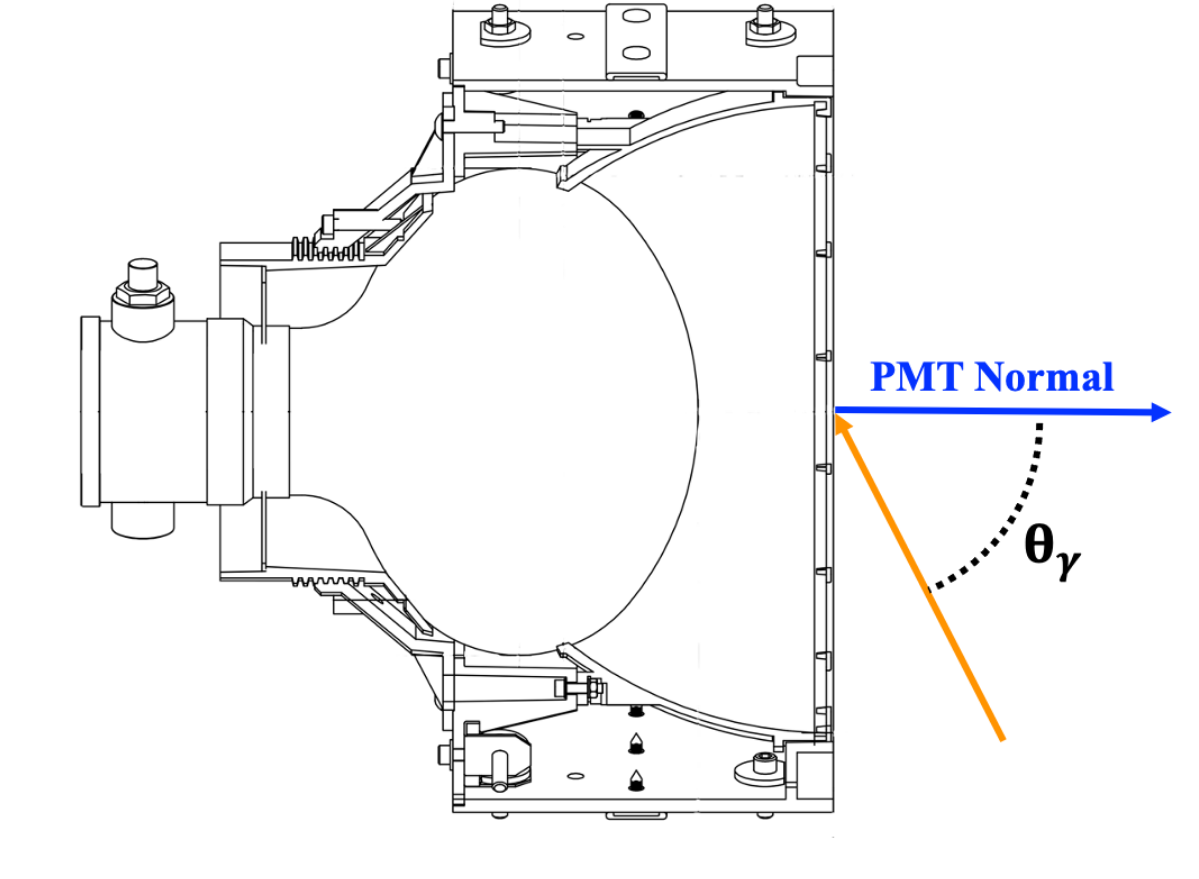
\includegraphics[width=0.95\textwidth]{2_Detector/Figs/pmt_bucket_assembly.png}
        \caption{}
        \label{fig:pmt_conc_diagram}
    \end{subfigure}
    \begin{subfigure}{0.69\textwidth}
        \centering
        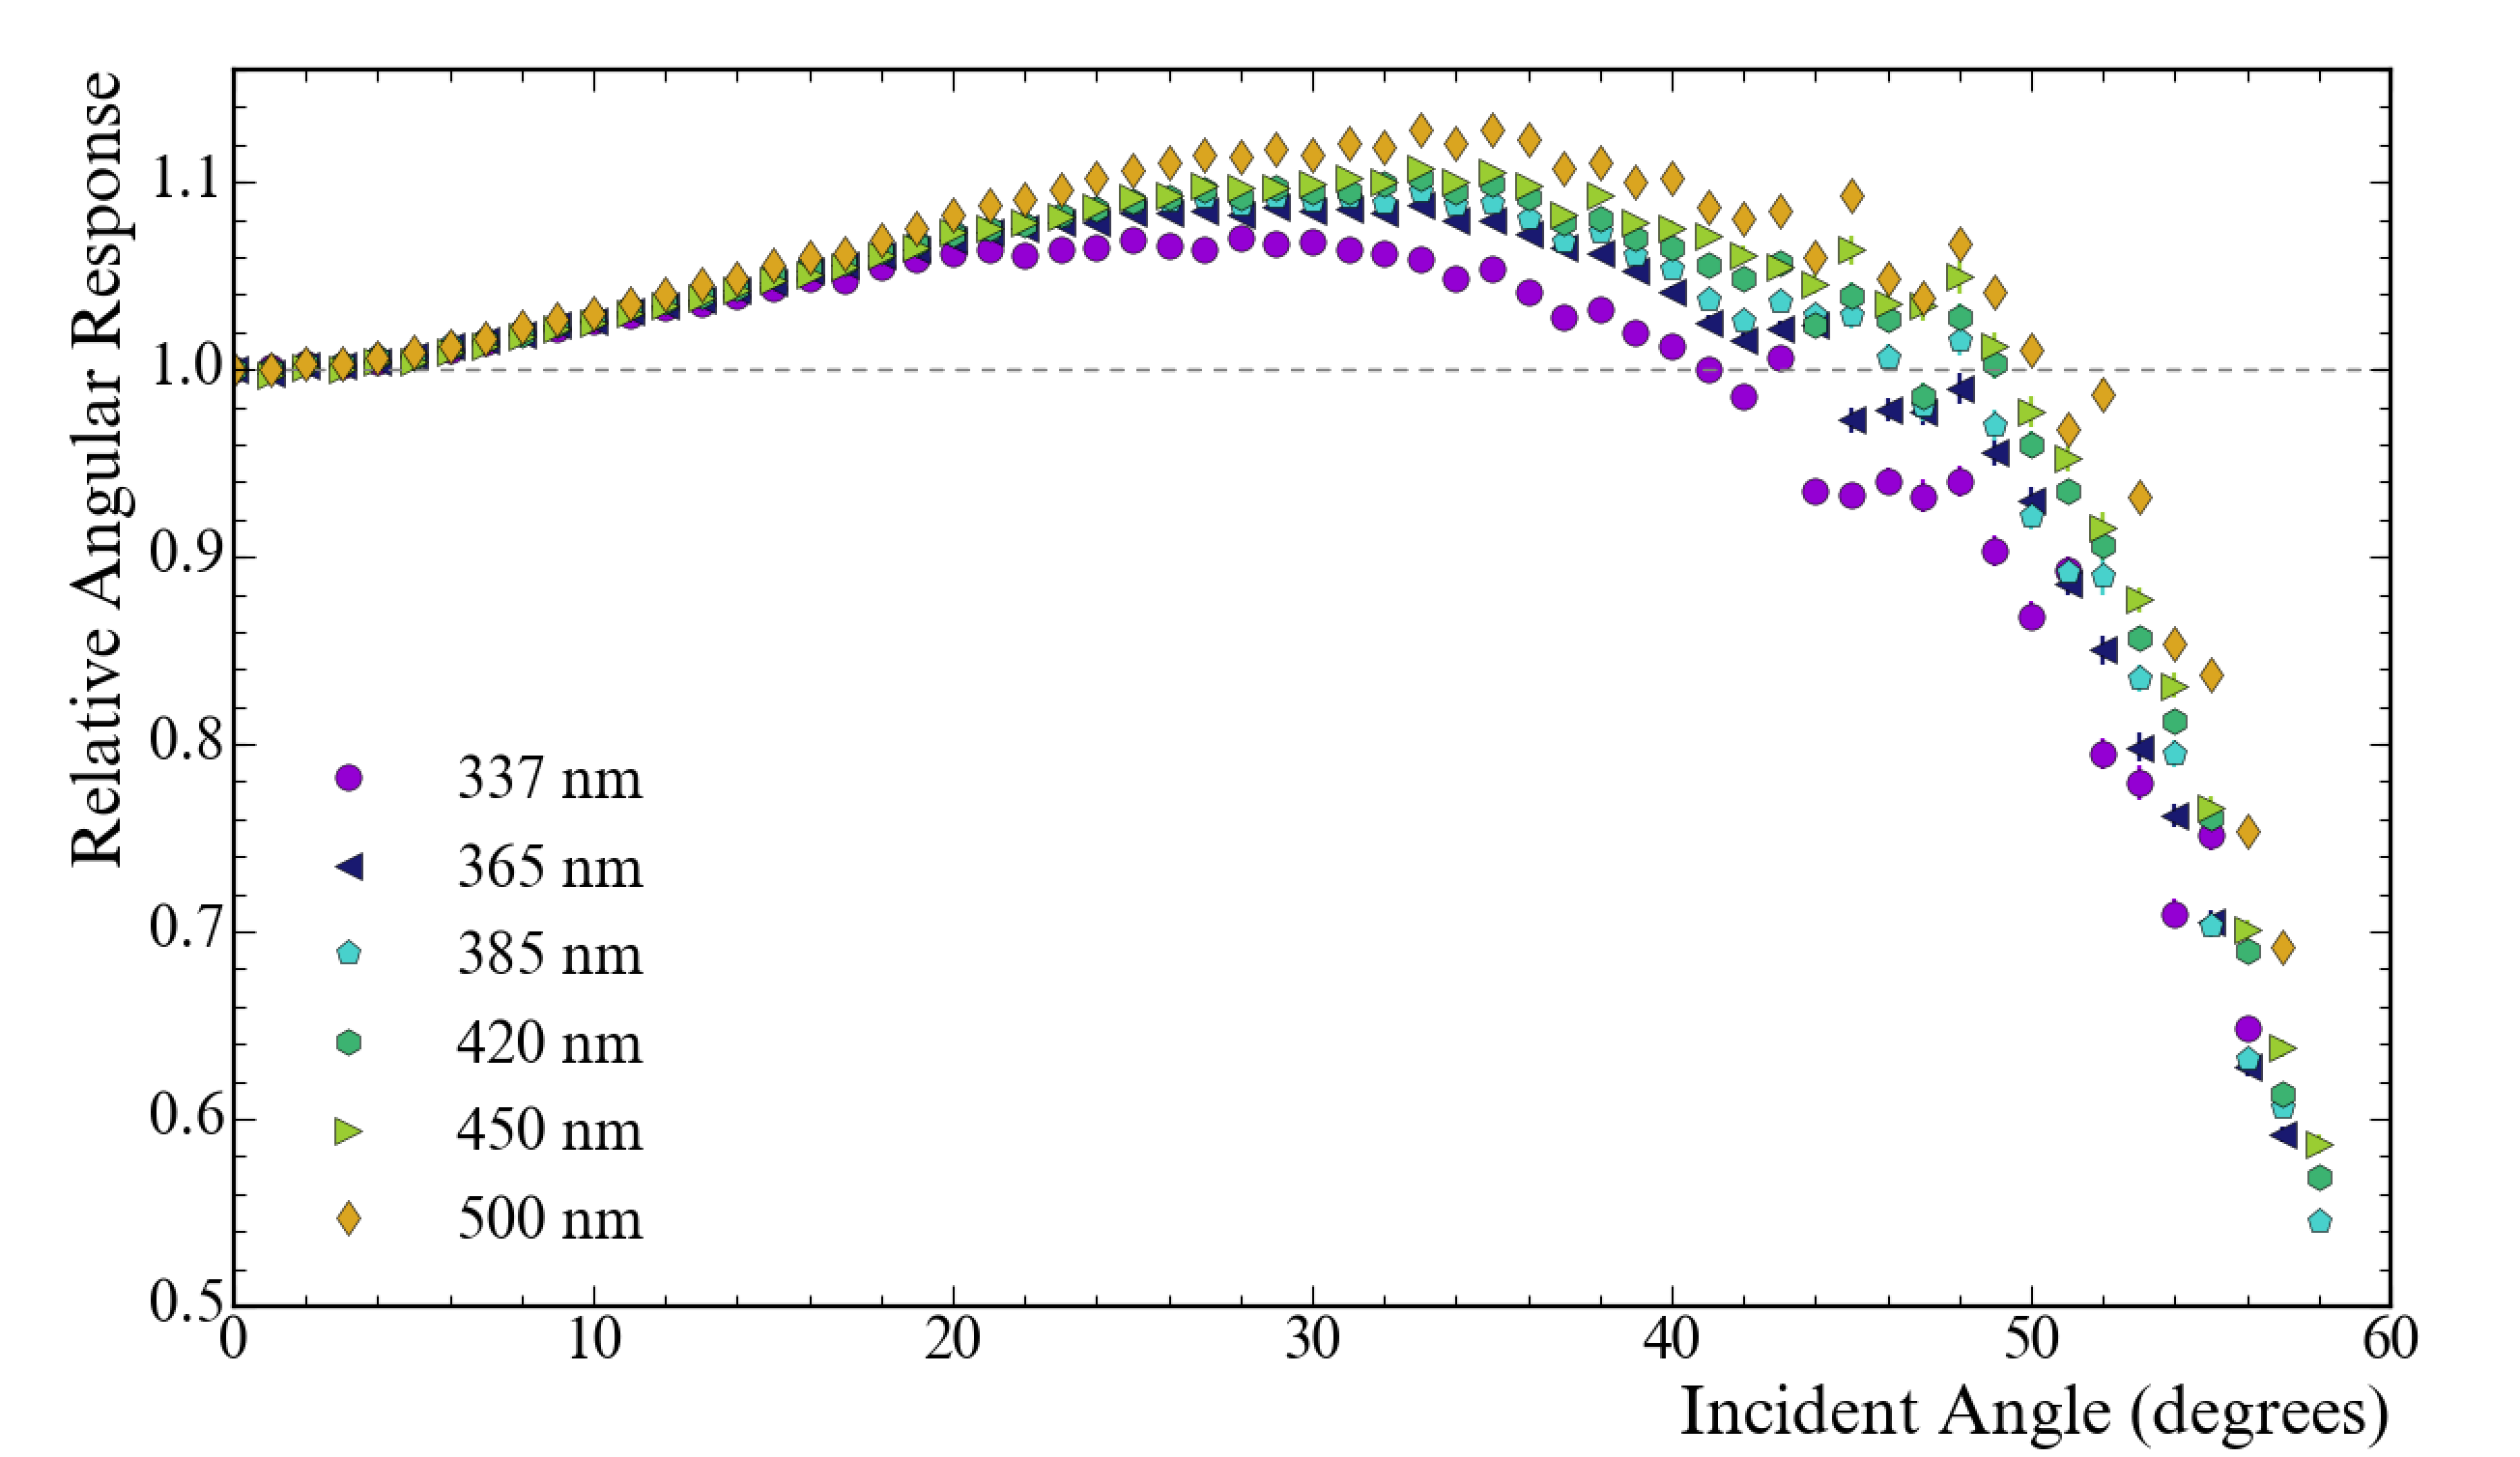
\includegraphics[width=0.95\textwidth]{2_Detector/Figs/PMTResponse.png}
        \caption{}
        \label{fig:pmt_angular_response}
    \end{subfigure}
    \caption[]{\textbf{(a):} Diagram of the PMT and concentrator `bucket' used within SNO+, showing also the definition of the incidence angle. \textbf{(b):} Plot of the measured relative angular response of the PMTs in SNO+, as a function of both incidence angle and wavelength. Both figures taken from~\cite{andersonOpticalCalibrationSNO2021}.
    }
    \label{fig:pmt_optics}
\end{figure}

\nomenclature{\textbf{QE}}{Quantum efficiency (of a PMT)}
\nomenclature{\textbf{TTS}}{Transit time spread (of a PMT)}
% \nomenclature{\textbf{FWHM}}{Full-width at half-maximum (of a distribution)}
Once a photon is incident on the PMT's photocathode, it is possible for that photon to be absorbed and generate a photoelectron. The probability of this happening is governed by the photocathode's Quantum Efficiency (QE) at the photon's wavelength, as well as the collection efficiency of a photoelectron onto the first dynode of the PMT. The combined measured efficiency of PMTs tested \textit{ex-situ} for SNO can be seen in Fig~\ref{fig:qe_pmts}. Once this photoelectron has been created, the dynodes within the PMT generate a cascade of electrons that produce an observable voltage signal. The dynamics of this cascade are such that there is a natural spread of possible times between the creation of a photoelectron and the generation of the voltage pulse in the PMT's anode. This is known as the `Transit Time Spread' (TTS) of the PMTs: for SNO+, the RMS of the TTS for the R1408-type PMTs is $\sim\SI{1.7}{\ns}$~\cite{BOGER2000172}. % cite SNO-era papers

\begin{figure}
    \centering
    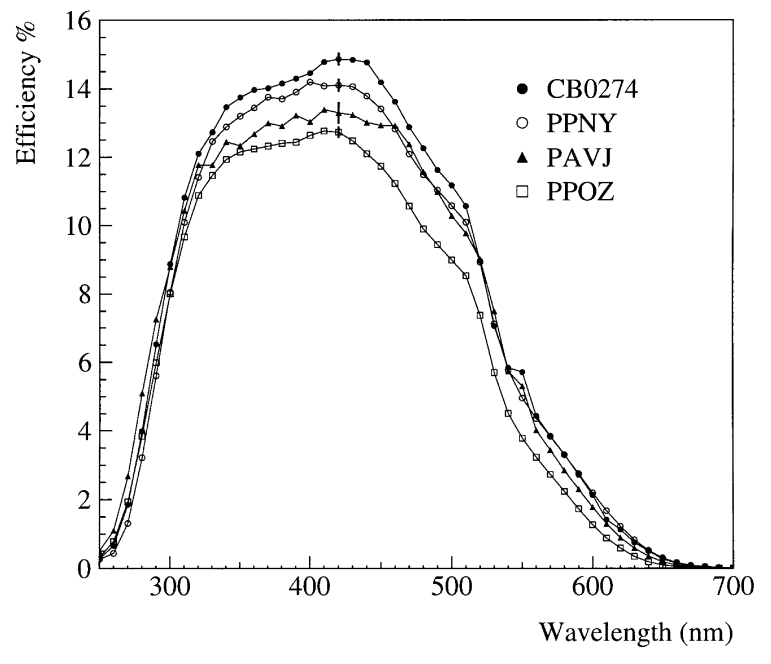
\includegraphics[width=0.7\textwidth]{2_Detector/Figs/efficiencies_PMTs_biller1999.png}
    \caption[Efficiencies of the R1408-type PMTs used as standard within SNO+]
    {Efficiencies of four R1408-type PMTs tested for calibration by~\cite{billerMeasurementsPhotomultiplierSingle1999}. % cite
    }
    \label{fig:qe_pmts}
\end{figure}

\nomenclature{\textbf{npe}}{Number of photoelectrons}
Finally, if multiple photons generate photoelectrons on the same PMT close enough in time, the amount of charge generated increases in proportion to the number of photoelectrons (npe). Much like with the transit time, the strength of the signal observed by the PMT is governed by a distribution, a function of the npe generated. Examples of these distributions can be seen in Fig.~\ref{fig:charge_dists_pmt}. % cite
The relatively large widths of these charge distributions precludes the ability to straightforwardly determine the npe purely from charge when the npe is small. To work around this, various techniques can be employed to try and estimate the npe in a given PMT --- an example of one such method can be seen in Section~\ref{sect:new_beam_profiles}.

\begin{figure}
    \centering
    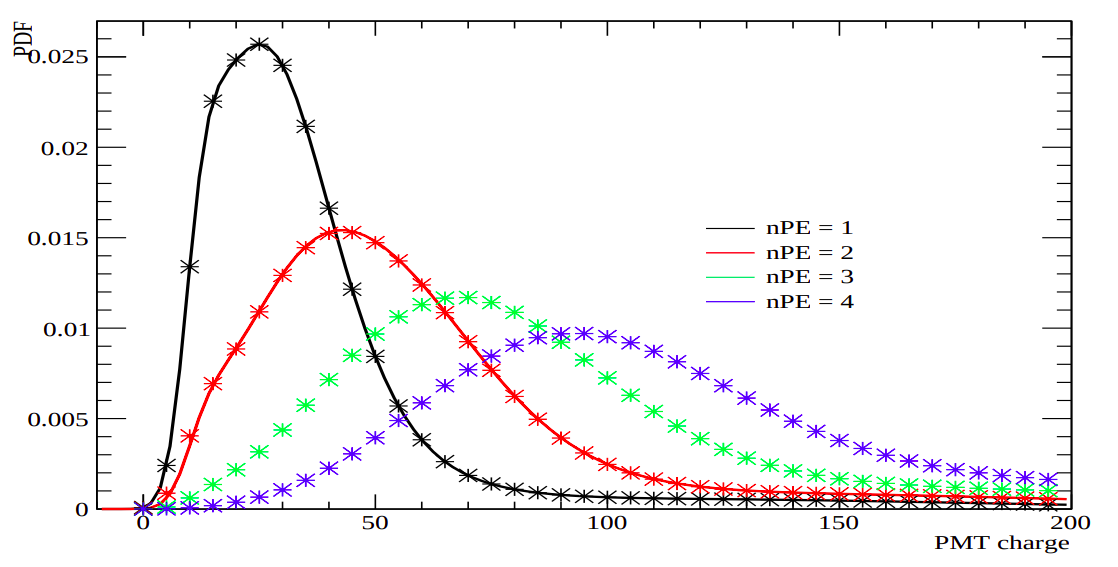
\includegraphics[width=0.8\linewidth]{2_Detector/Figs/charge_spectra_mod.png}
    \caption[Example charge spectra for a PMT as a function of the true npe generated]{Example charge spectra for a PMT as a function of the true npe generated. Figure taken from~\cite{dungerOccupancyAnalysisMultipleHit2016}. % cite whom?
    }
    \label{fig:charge_dists_pmt}
\end{figure}


    % \begin{itemize}
    %     \item Light gets detected via the PMTs. Note the existence of the PMT concentrators to maximise coverage within the AV, but minimise it in the external water: show the calibrated angular response.
    %     \item Remind reader that a PMT converts photons to photoelectrons with a certain quantum efficiency, dependent on the wavelength of light.
    %     \item The process of multiplying the signal induces a spread in the possible generated time of the voltage signal, known as the PMT's transit time spread.
    %     \item The PMT response is also weakly dependent on the number of photoelectrons generated; not enough to be able to confidently distinguish the npe under most circumstances.
    % \end{itemize}
    % [2 pages]
\subsection{Data Acquisition and Triggering}\label{sec:daq}
\nomenclature{\textbf{DAQ}}{Data acquisition (system)}
Once a signal reaches the cable attached to a PMT, it travels along up to the front-end electronics on the deck above the detector. The job of these electronics, known as the data acquisition (DAQ) and triggering system, is to convert raw electronic signals from the PMTs into recorded digital `events' that can be used for analysis. A schematic showing the setup of the electronics is shown in Fig~\ref{fig:tdaq_schematic}, with full details in~\cite{albaneseSNOExperiment2021}. % cite

\begin{figure}
    \centering
    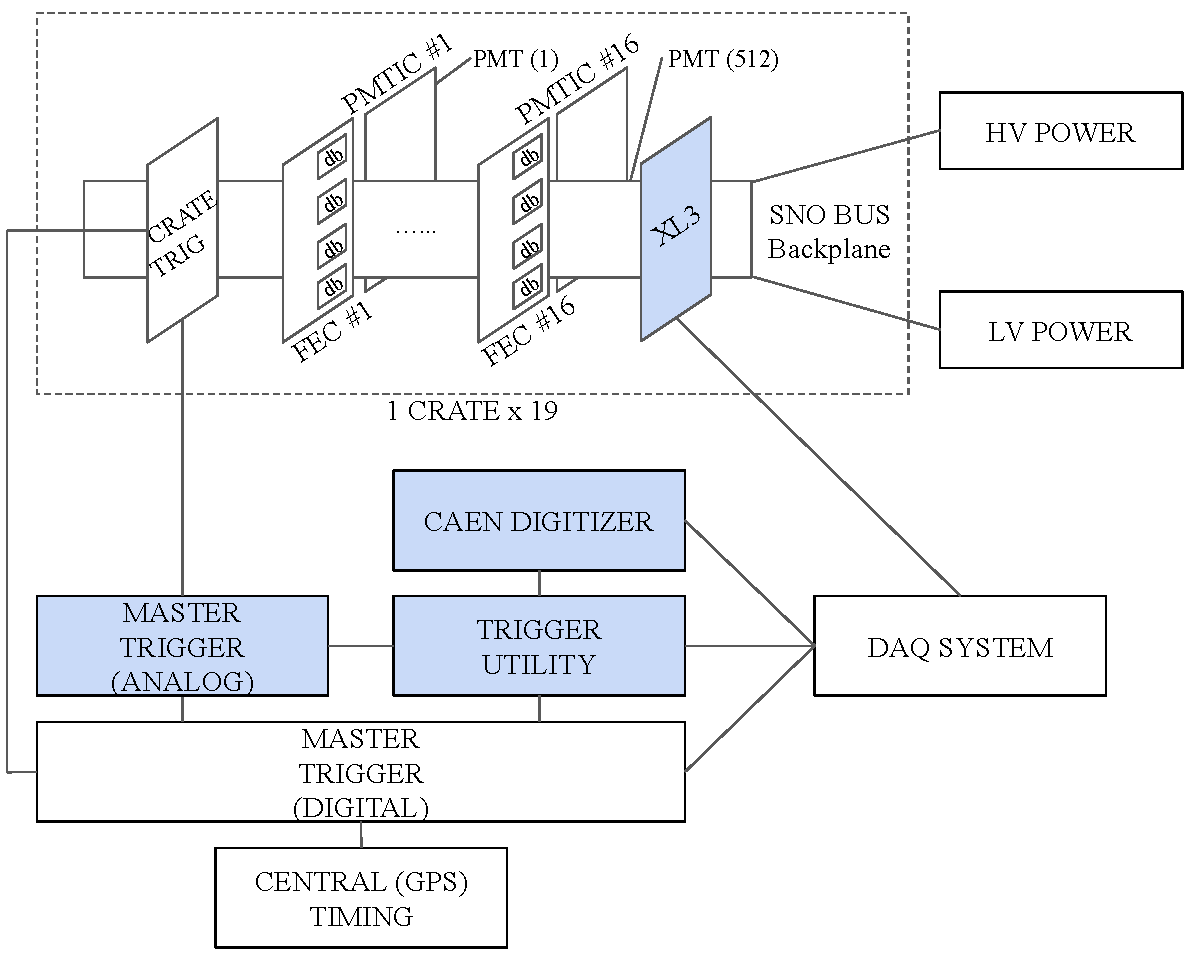
\includegraphics[width=0.7\linewidth]{2_Detector/Figs/electronics_diagram.pdf}
    \caption[Schematic of the front-end electronics used for data acquisition and triggering in SNO+]{Schematic of the front-end electronics used for data acquisition and triggering in SNO+, taken from and discussed in~\cite{albaneseSNOExperiment2021}. % cite
    }
    \label{fig:tdaq_schematic}
\end{figure}

\nomenclature{\textbf{PMTIC}}{PMT Interface Card}
\nomenclature{\textbf{DB}}{Daughter Board}
\nomenclature{\textbf{FEC}}{Front-End Card}
\nomenclature{\textbf{TAC}}{Time-to-amplitude Converter}
\nomenclature{\textbf{QHS}}{Charge with high gain over a `short' integration time (\SI{60}{\ns})}
\nomenclature{\textbf{QHL}}{Charge with high gain over a `long' integration time (\SI{390}{\ns})}
\nomenclature{\textbf{QLX}}{Charge with low gain over a `long' integration time (\SI{390}{\ns})}
A signal passes first through the PMT Interface Card (PMTIC), which then sends it through to one of the Daughter Boards (DBs) which are stored on Front-End Cards (FECs) within one of 19 electronic crates on deck. The DBs determine if the analogue signal along a given PMT channel has crossed a pre-defined charge threshold, at which point we say that we have detected a `hit' on that PMT's channel. When this occurs, the DB performs a set of important actions:
\begin{enumerate}
    \item Begins a timer for that channel, in the form of a Time-to-Amplitude Converter (TAC). TAC also corresponds to the resulting analogue voltage on the output of the TAC being measured.
    \item Begins integrating the total charge signal for that channel in three ways, known as QHS, QHL, and QLX. These correspond to using different integration times and gain settings.
    \item Generates trigger pulses for that channel for each available trigger type. Three main trigger signals are the `N20' (a square pulse for \SI{20}{\ns}), `N100' (a square pulse for \SI{100}{\ns}), and `ESUMHI' (a pulse copying the shape of the voltage signal for that channel). The reason for these names will be explained shortly.
\end{enumerate}

\nomenclature{\textbf{CTC}}{Crate Trigger Card}
\nomenclature{\textbf{MTC/A+}}{Analogue Master Trigger Card}
Whilst the TAC, QHS, QHL, and QLX are being calculated, the trigger signals from each channel are sent over to the Crate's Trigger Card (CTC), where the signals are then summed for each trigger type. These crate-level trigger signals are then sent over to the 7 detector-level Analogue Master Trigger Cards (MTC/A+), which further sum the signals by trigger type from all the crates in the detector. It is at this point of the process where the names of the trigger types becomes clear: the combined N20 and N100 signals are proportional to the total number of hit PMTs within a \SI{20}{\ns} and \SI{100}{\ns} time window, respectively, whilst the total ESUMHI signal corresponds to the total charge seen over all the PMTs.

\nomenclature{\textbf{MTC/D}}{Digital Master Trigger Card}
\nomenclature{\textbf{GT}}{Global Trigger}
\nomenclature{\textbf{EXTA}}{External Asynchronous (Trigger)}
\nomenclature{\textbf{TUBii}}{Trigger Utility Board Mark ii}
If these trigger signals go above certain pre-defined thresholds, then a signal is sent for that trigger type to the Digital Master Trigger Card (MTC/D). The MTC/D receives all trigger signals from the detector, and if a given trigger type has been `masked in' (i.e. activated) the Card will generate a Global Trigger (GT) for the detector with a time stamp from its \SI{50}{\MHz} clock. Under certain circumstances, such as calibrations, a trigger signal can be generated externally and asynchronous to the MTC/D: these are `EXTA' triggers. Any such EXTA trigger signal is first handled by an electronics box named `TUBii' (Trigger Utility Board Mark ii), before then being passed onto the MTC/D. TUBii functionality will become relevant when discussing the calibration electronics described in Chapter~\ref{chap:smellie_hardware}.

\nomenclature{\textbf{ADC}}{Analogue-to-Digital Converter}
Once a GT signal is generated, it is then sent back to all the CTCs, which then orders the integration of time and charge to be stopped on all channels for that crate. The time and charge information that has been temporarily stored on each channel's CMOS chip on the FEC is then sent to the crate's `XL3' card, which packages the crate's raw information via ethernet over to a set of computers. The trigger signals for a triggered event are also digitised by a CAEN brand Analogue-to-Digital Converter (ADC), and sent to the same DAQ computers. The total window of time in which data is gathered from one GT signal is \SI{400}{\ns}, with data from up to \SI{180}{\ns} before and \SI{220}{\ns} after the GT has arrived. There is then a necessary `dead time' of \SI{420}{\ns} after a given GT has been given in which no further GTs can be made.

\nomenclature{\textbf{ZDAB}}{Zebra Database (file format)}
\nomenclature{\textbf{GTID}}{Global Trigger Identification number}
Finally, the raw data from the crates and trigger system arrives in a set of computers, which organise all of this into an individually-packaged `event', stored on disk in the `Zebra Database' (ZDAB) format. A given built event contains the TAC and charge information from each hit PMT, the CAEN digitised waveforms, a unique identifying number for that triggered event (the GTID), as well as the times from both the MTC/D's \SI{50}{\MHz} clock and a GPS-calibrated \SI{10}{\MHz} clock. The former time is used for measuring relative times between events whilst the latter is used for knowing the time of day of an event: both are used in Chapter~\ref{chap:solar_osc_analysis}.


    % \begin{itemize}
    %     \item Summarise how a PMT signal becomes digitised via the front-end electronics, briefly.
    %     \item Summarise the triggering system, as I'll have to describe in a later chapter how the SMELLIE hardware fits into this, especially as there have been ongoing SMELLIE triggering issues worth mentioning there!
    %     \item Note the information stored by an event: importantly for this thesis, the TAC and QHS per hit, the event's GTID as well as trigger time measured from the \SI{50}{\mega\Hz} clock. The latter is worth mentioning as this is how I determine time differences for my BiPo tagging in the solar analysis.
    %     \item Finally, note that these get written to file in the ZDAB format.
    % \end{itemize}
    % [3 pages]
\subsection{Operation of the Detector}\label{sec:detector_ops}
Control of the detector's DAQ system is handled through a custom-built GUI known as ORCA~\cite{howeSudburyNeutrinoObservatory2004}. %cite
This program allows operators of the detector to modify settings in the detector electronics at both a low- and high-level. It also allows operators to monitor the current status of the detector, such as voltage and current levels within each crate.

ORCA allows for the detector to have its data split into `runs' of different types. For the majority of the time, the detector is run in the `Physics' mode, with individual runs split into 1 hour periods. It is this data that is used for almost all high-level physics analyses, such as the one described in Chapter~\ref{chap:solar_osc_analysis}. To help with the movement and processing of data, runs of raw data are split into ZDAB files of maximum size \SI{1}{\giga\byte}. Because of this, the number of files generated per run is proportional to the trigger rate of the detector. In the current \SI{2.2}{\gpl} LABPPO scintillator phase under nominal conditions, the trigger rate is $\sim\SI{2.5}{\kilo\Hz}$, leading to 15 ZDAB files being generated per run of 1 hour in length.

Other detector run types include ones for detector maintenance, as well as for calibrations of various kinds. During certain calibration runs, data can be further split into `subruns' where necessary. This allows for data taken from a given calibration source to have the different settings used (e.g. different wavelength settings) all kept within one run, but still appropriately separated. Operation of specific calibration sources, including the one described in Chapter~\ref{chap:smellie_hardware}, can be performed through the ORCA GUI.


    % \begin{itemize}
    %     \item Detector electronics operated through ORCA; allows for different running modes, such as calibrations.
    %     \item Mention that data gets split into run and subruns.
    % \end{itemize}
    % [1 page]
\section{Calibrations and Detector Modelling}\label{sec:calibs_modelling}
Once the raw data from triggered events has been stored in files, certain extra steps must be taken before effective analysis of that data can be achieved. This section covers those steps.

\subsection{Detector Monitoring}
No data taken from the detector can reasonably be used for analysis unless its quality has been approved. This is done in a number of ways on SNO+. Firstly, a number of automated systems monitor all aspects of the detector, including voltage levels in the crates, trigger rates, as well as `slower' quantities such as the tensions on the ropes holding the AV in place. Problems in any of these measured parameters trigger an automatic alarm system, which notifies a human detector operator. A human detector operator monitors the detector 24/7 whilst the detector is live.

\nomenclature{\texttt{RATDB}}{RAT Database}
In addition to systems that monitor whether anything has gone wrong, information about the state of the detector during each run is stored in a database known as \texttt{RATDB}. This information includes, amongst other things, a recording of which PMT channels have actually been raised to high voltage for that run, as well as any channels/cards/crates that have been flagged for having a known poor data quality (e.g. being overly noisy).


    % \begin{itemize}
    %     \item Detector's state is continuously monitored via a number of systems for data quality purposes, including a human detector `shifter'. This includes the alarm systems for the electronics and slow controls, and `nearline' monitoring of the detector status.
    %     \item CHS and CSS ensure only ``good'' channels used in any analysis.
    % \end{itemize}
    % [1 page]
\subsection{Electronic and PMT Calibrations}
\nomenclature{\textbf{ECA}}{Electronic Calibration}
\nomenclature{\textbf{PCA}}{PMT Calibration}
The lowest level of calibrations performed in SNO+ are the Electronic and PMT Calibrations: ECAs and PCAs, respectively. These calibrations convert the raw time and charge values recorded by the DAQ into quantities that can actually be used in analysis.

During an ECA, two main quantities are measured. Firstly, because of noise the integrated charge measured on each channel is offset by some amount. This offset, known as the `pedestal', is recorded for each channel. The other quantity is the `time slope' for each channel, which allows one to convert from the ADC TAC counts into an uncalibrated hit time of that channel's PMT in \si{\ns}. Both of these quantities are measured by sending external signals to channels in the crates, forcing them to start measuring TAC and charge even though no PMTs were actually hit. Running ECAs also enable us to spot any channels with unusual behaviour, so that they are not used during analysis. ECAs are typically done on a fortnightly basis, or after maintenance to the DAQ system has been performed.

Using ECAs alone is not enough to have fully-calibrated time and charge data. The lengths of cables between PMTs and PMTICs are all slightly different, leading to differences in the so-called `cable delay' of each channel. This means that two PMTs that have a photoelectron generated at the same time can generate slightly different TAC values. Furthermore, because the start time of the TAC is determined by when the channel's signal goes above a constant threshold, if a signal is very large (e.g. when numerous photoelectrons have been generated on one PMT) then the start time of the TAC will be systematically earlier. This is known as the `time walk'. Both of these quantities get measured during PCAs.

\nomenclature{\textbf{ELLIE}}{Embedded LED/Laser Light Injection Entity}
\nomenclature{\textbf{TELLIE}}{Timing subsystem for ELLIE}
PCAs can be performed by either the Laserball or by the TELLIE calibration system. The latter is a series of 92 optical fibres attached at various points of the PSUP, through which optical-wavelength light can be fired from LEDs. TELLIE is the Timing subsystem of the ELLIE calibration system: the Embedded LED/Laser Light Injection Entity. The other two fibre-based optical calibration subsystems, AMELLIE and SMELLIE, are introduced in Section~\ref{sec:eo_calibs}. For both the Laserball and TELLIE calibration systems, the cable delay and time walk are measured by firing light from the source at a known time and with a known hit occupancy, and observing when the signal arrives in each PMT channel.

On top of calibrating the PMT hit times, PCAs also further calibrate the charge information. In particular, the charge spectrum generated by a single photoelectron is determined for each channel. This allows us to convert the pedestal-corrected charge ADC counts into an approximate number of photoelectrons.

Using the data gathered from both ECAs and PCAs, the raw data stored in \texttt{ZDAB}s is processed into a new file format known as \texttt{RATDS} files. These files contain all the information of an event, but now the timing and charge information have been calibrated. It is this file type used in the optical calibration work of Chapters~\ref{chap:smellie_hardware}--\ref{chap:smellie_analysis}.

    % \begin{itemize}
    %     \item First main set of calibrations are the ECAs and PCAs. These help us convert raw electronic signal information from PMTs into `calibrated' hit times and charges. PCAs performed via TELLIE and the Laserball.
    %     \item These initial calibrations allow for the first two passes of data processing, resulting in a `RATDS' file format used in optical calibrations.
    %     \item No need for many details here; this is not a thesis on this topic!
    % \end{itemize}
    % [1 page]
\subsection{Energy and Optical Calibrations}\label{sec:eo_calibs}
The next stage of calibrating the detector is modelling its optical properties. These properties include all the processes covered in Section~\ref{sec:optical_processes}, such as scintillator emission, optical absorption, re-emission, and Rayleigh scattering.
This is crucial, as it allows us to reconstruct information about events within the detector: more on event reconstruction shortly.

\nomenclature{\textbf{AMELLIE}}{Attenuation Module for ELLIE}
\nomenclature{\textbf{SMELLIE}}{Scattering Module for ELLIE}
In addition to deployments of the Laserball (discussed in Section~\ref{sec:optical_processes}), two further calibration sources are used in SNO+ to measure properties of light propagation: AMELLIE and SMELLIE. These are the `Attenuation Module' and `Scattering Module' for the ELLIE calibration system. Like TELLIE, AMELLIE and SMELLIE consist of optical light sources that shine through optical fibres into the detector. The former uses LEDs from TELLIE, whilst the latter uses optical wavelength lasers. Despite the names both subsystems are similar enough that they are both capable of measuring attenuation and scattering within the detector. More details about the SMELLIE hardware can be read in Chapter~\ref{chap:smellie_hardware}.

\nomenclature{\textbf{AmBe}}{Americium-Beryllium radioactive source}
Another critical component of the detector to calibrate well is the energy response: given a specific amount of energy deposited in the water/scintillator, how many hits are observed? For this, a number of radioactive sources are used at a variety of energies. In the scintillator phase, there are three main sources. The first is an americium-beryllium (AmBe) source inherited from SNO~\cite{loachMeasurementFlux8B2008}, % SNO AmBe paper
which contains \ce{^{241}Am} that $\alpha$-decays, which can be captured by the \ce{^{9}Be} within the source. This capture leads to the emission of a neutron as well as production of a \ce{^{12}C} nucleus, which 60\% of the time is in  an excited state. When this excited state decays, a \SI{4.4}{\MeV} $\gamma$ is emitted promptly. Eventually the neutron is captured by hydrogen in the detector, leading to a characteristic \SI{2.2}{\MeV} delayed $\gamma$ being generated~\cite{albaneseSNOExperiment2021}. % cite detector paper
Both the prompt and delayed peak energies from the AmBe source can be used for energy calibration. In addition to this, one can calibrate the neutron detection efficiency with the AmBe source~\cite{loachMeasurementFlux8B2008}, % cite AmBe paper
which is important for the analysis of antineutrino IBD events. % CONFIRM IBD acronym in chapter 1

Another deployable radioactive source is the \ce{^{16}N} source, also originally used for SNO~\cite{dragowsky16NCalibrationSource2002}. % SNO N16 paper
The \ce{^{16}N} isotope $\beta$-decays to \ce{^{16}O}, with a distinctive \SI{6.1}{\MeV} $\gamma$ also being generated 66\% of the time. It is the $\gamma$ that can make it out to the detector, whilst the $\beta$ can be tagged by a block of scintillator and PMT held within the source container.

In theory, sources can be deployed both within the AV (`internally') and in the water shielding (`externally'). Both internal and external deployments were used for the optical calibration of the water phase with the Laserball~\cite{andersonOpticalCalibrationSNO2021}. Although external deployments during the scintillator phase with the Laserball, N16, and AmBe sources have been made, there have been no such internal source deployments. This is a result of the substantial work currently underway~\cite{valderLaserballCalibrationDevice} to overhaul the internal deployment hardware, in order to satisfy the much more stringent radiopurity requirements of the scintillator phase over the water phase.

Alongside these deployed sources, a different kind of radioactive source has been used during the scintillator phase for energy calibration: the existing radioactive background spectra within the detector. Backgrounds such as \ce{^{14}C}, \ce{^{210}Po}, \ce{^{214}BiPo}, and \ce{^{208}Tl} all have distinctive peaks in the energy spectrum of SNO+ during the scintillator phase, and can be used to calibrate the scintillator's energy response. Using \ce{^{214}BiPo} events in particular has been used for energy scale calibration with the solar oscillation analysis, as discussed in Section~\ref{sec:exp_rates_constraints}.

    % \begin{itemize}
    %     \item After ECAs and PCAs, further calibration is necessary to accurately model the optical properties of the detector.
    %     \item Describe briefly the function of the Laserball, SMELLIE, and AMELLIE sources in optical calibration (can reference the water-phase optical calibration paper). Details of how each analysis works is obviously not needed here, especially not for SMELLIE as we have 3 chapters to go over that!
    %     \item AmBe and N16 sources provide further information for calibration
    %     \item In-situ backgrounds used for more calibration sources, especially for determining the light yield of the scintillator, and Birks' constant.
    % \end{itemize}
    % [2 pages]
\subsection{Event Reconstruction}\label{sec:ev_reco}
Once the detector has been calibrated, event `reconstruction' becomes possible. This is the process of deriving high-level physics quantities about a triggered event within the detector, based upon the calibrated hit information. In SNO+, our base assumption in most cases of event reconstruction is that a triggered event was due to a single electron track. Reconstructing an event involves running a number of algorithms, which in the scintillator phase are together called the \texttt{ScintFitter}.

\nomenclature{\textbf{TOF}}{Time-of-flight (of a photon)}
The first critical pieces of information that gets determined by \texttt{ScintFitter} is the event's position and time. The reconstructed position corresponds to the point in the detector where the triggered event most likely came from (assuming the event was approximately point-like in extent), whilst the reconstructed time is the starting emission time of the event, relative to the event's trigger time. The position of an event is critical to know, as far fewer background events occur near the centre of the detector compared to the edges. It is also important to know the emission time of an event, as this allows us to build the so-called `time residual' (\tres{}) distribution of an event. For a point-like physics event in the detector, \tres{} for a given PMT hit is defined as:
\begin{equation}
    \tres = t_{\mathrm{hit}} - t_{\mathrm{TOF}} - t_{\mathrm{emm}},
\end{equation}
where $t_{\mathrm{hit}}$ is the calibrated hit time of the PMT, $t_{\mathrm{TOF}}$ is the time one expects for light to travel directly from the reconstructed position to that PMT (the time-of-flight), and $t_{\mathrm{emm}}$ is the reconstructed emission time.

Whilst a number of algorithms have been developed for reconstructing position and time in SNO+, they all work on the same basic principle. Because of the spherical symmetry of the detector, if an event occurs at the centre of the detector one expects direct light to hit PMTs throughout the detector at the same time\footnote{It is possible for the centre of the AV and PSUP to not be completely aligned, i.e. there is an `AV offset'. Then, the spherical symmetry can be very slightly broken by refraction through the AV. Fortunately, we account for this when coordinating our position fitters.}.
However, if an event happens some distance away from the detector's centre then direct light will arrive at the PMTs it is closer to sooner. Therefore, by looking at the distribution of hit times for PMTs that were hit earliest as a function of the PMTs' positions in the detector (ignoring PMT hits that arrived much later, presumably because the photon paths were not direct) one can try and estimate where the position of the event was. Reconstructed positions and reconstructed times are linked by the time residual equation described above.

Currently on SNO+, a likelihood-based approach is used to reconstruct position and time. The algorithm endeavours to maximise the combined likelihood of the observed calibrated hit times of the hit PMTs, given proposed points in the four-dimensional (position, time) parameter space~\cite{jonesBackgroundRejectionNeutrinoless2011,coulterModellingReconstructionEvents2013,parkerMultiPDFMethodPosition2021}. % cite Multipath thesis
However, regardless of algorithm there are two factors that limit the position and timing reconstruction of an event. The TTS of the PMTs used as well as the speed of the scintillator emission timing defines the fundamental timescale --- and hence also length scale --- by which events can be reconstructed. Secondly, if more photons are able to generate prompt hits in the detector from a given event, then more information can be used to determine the position and time. Under current conditions, a \SI{2.5}{\MeV} event in the centre of the detector will have a position resolution of \SI{100}{\mm}~\cite{parkerRecoordinatingScintEffectiveSpeedMultiPDF2023}. % TODO & cite Will's recoordination!

The other critical piece of reconstructed event information is the event's energy. More precisely, this is the kinetic energy of an electron that has been assumed to have generated the event. By consequence, events due to $\alpha$-decay will obtain reconstructed energies well below the actual energy of the $\alpha$ particle, because of scintillator quenching (see Section~\ref{sec:scintillation} for details).

\nomenclature{\texttt{nhit}}{Number of PMT hits in an event}
At its simplest, assuming that an event is from an electron of moderate energy (e.g. at \SI{2.5}{\MeV}), then we can expect the number of PMT hits observed to be directly proportional to the energy of the event. Given that the number of hits observed in an event (called the \texttt{nhit}) is governed by a Poisson distribution, then the uncertainty in energy will just be proportional to the square root of the number of hits. As a result, the reconstructed energy resolution in SNO+ is determined by the scintillator's light yield and absorption length, as well as the coverage and QE of the PMTs.

There are second-order corrections to the energy reconstruction that need to be considered to minimise bias. At low energies, scintillator quenching becomes non-negligible, so an understanding of the scintillator's Birks' constant is needed. At high energies, many PMTs will have had multiple photoelectrons generated, so merely using the \texttt{nhit} will give an underestimate of the true energy. Finally, the detection efficiency of photons is non-uniform as a function of position in the detector. The current energy reconstruction algorithm used within SNO+ attempts to deal with all of these effects~\cite{mottramUpdatedFunctionalForm2015,kroupovaImprovingSensitivityNeutrinoless2020}. % cite energy reco info

After position, time, and energy reconstruction, \texttt{ScintFitter} calculates a number of additional quantities from what are known as classifiers. These describe a wide number of properties about an event, often using the derived \tres{} distribution of an event as the basis for classification. Some examples of classifiers used in analysis are discussed in Section~\ref{sec:background_processes}.

All Physics data runs, as well as certain calibration data such as AmBe and \ce{^{16}N}, has the \texttt{ScintFitter} algorithm run over it after having been processed for time and charge calibration. This results in what is known as a fully-processed \texttt{RATDS} file, as well as a new file type known as an \texttt{ntuple}. This latter file type has much of the hit-level information removed, and contains only event-level information such as the reconstructed energy and position. Because these files are much smaller, they are the ones typically used in the high-level physics analyses on the experiment, such as the one described in Chapter~\ref{chap:solar_osc_analysis}.


    % \begin{itemize}
    %     \item Once detector is calibrated, event reconstruction becomes possible. Describe main assumption of a SNO+ event: we assume a single-site electron event.
    %     \item Briefly describe the basics of how energy, position, and time reconstruction works, as this is needed for the solar analysis chapter. Mention existence of direction fitting in scintillator!
    %     \item `Physics' runs have their events reconstructed in a third pass of data processing, resulting in a `fully-processed' RATDS file as well as a simplified NTUPLE file used in high-level physics analyses (such as my solar analysis).
    % \end{itemize}
    % [2 pages]
\subsection{Event Simulation}
\nomenclature{\texttt{RAT}}{Reactor Analysis Tool}
Simulations of events in SNO+ are performed using the software \texttt{RAT}~\cite{albaneseSNOExperiment2021}. % cite
Built on the \texttt{GEANT4} particle physics software framework, \texttt{RAT} is capable of simulating all aspects of the physics of an event within the detector via a Monte Carlo (MC) approach. This includes any particle physics that defines an event's generation, propagation and interactions of those particles in the detector media, the generation of light by both scintillation and Cherenkov processes, the propagation of that light, as well as the detection of that light by PMTs and simulation of the expected DAQ response. \texttt{RAT} is then used to process both simulation and data in the same way. In addition to being highly customisable, \texttt{RAT} can use the \texttt{RATDB} tables generated from a given data run when simulating to try and match those particular run conditions as closely as possible. \texttt{RAT} also offers a suite of tools to assist with analysis of data. The software is constantly being updated with new features --- the work done in this thesis uses \texttt{RAT} versions between 6.18.8 and 7.0.9, inclusive.

% {
%     \color{blue}
%     \begin{itemize}
%         \item Briefly describe overview of RAT software: not only provides the software by which the above data processing occurs, but allows for a GEANT4-based simulation of events in the detector. This simulation includes all parts of the physics described in Section~\ref{sec:event_journey}, including particle and nuclear physics interactions, optical photon creation and propagation, signal generation and event building based on simulated triggers of the electronics. These simulated events then get processed in the same manner as actual data is.
%     \end{itemize}
%     [1 page]
%     [24 PAGES TOTAL]
% }
\chapter{The SMELLIE Calibration System}\label{chap:smellie_hardware}
\epigraph{\textit{There's a certain Slant of light,\\
Winter Afternoons ---\\
That oppresses, like the Heft\\
Of Cathedral Tunes ---}}{\textsc{Emily Dickinson}}

As mentioned in Section~\ref{sec:eo_calibs}, one of the principal systems for calibrating the optics of the SNO+ detector is SMELLIE. This calibration device consists of 5 different optical wavelength lasers able to be fired through 15 optical fibres, whose endpoints are attached to the PSUP. A collimator is attached at the end of each fibre, ensuring the emitted light forms a narrow beam across the detector. A diagram of SMELLIE in the detector is shown in Fig.~\ref{fig:smellie_diagram}.

\begin{figure}
    \centering
    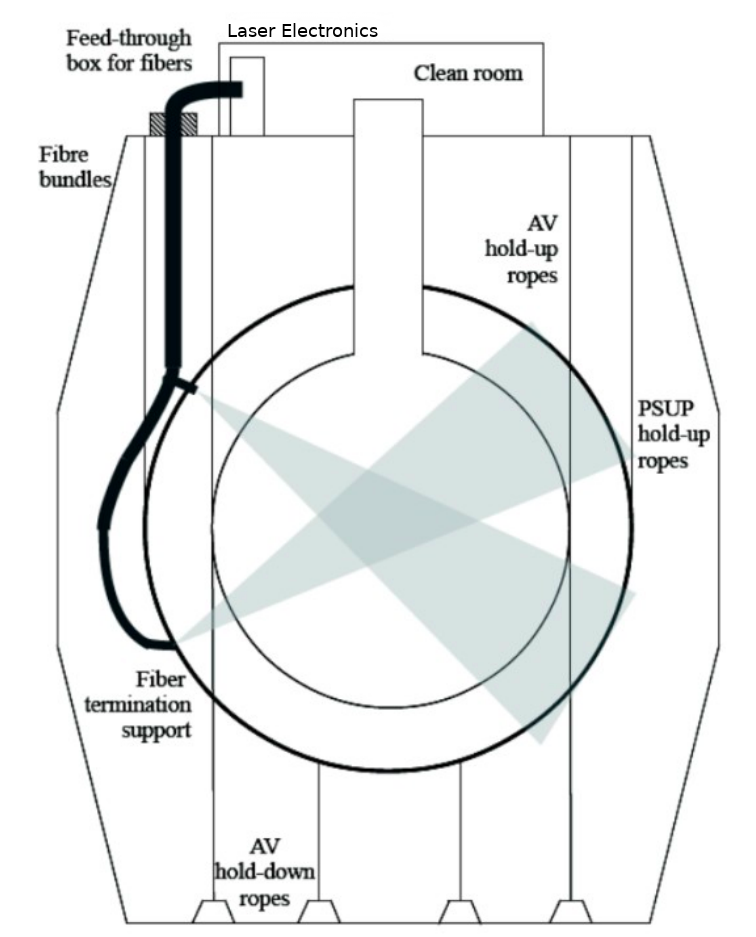
\includegraphics[width=0.48\textwidth]{3_SMELLIEHardware/images/SMELLIE_picture_corrected.png}
    \caption[Diagram of the SMELLIE calibration system within SNO+]
    {Diagram of the SMELLIE calibration system within SNO+. Modified from~\cite{sinclairPositioningTimingCalibration2015}.}
    \label{fig:smellie_diagram}
\end{figure}

The primary goal of SMELLIE is the measurement and monitoring of optical scattering within the detector over the lifetime of the experiment. By firing light from SMELLIE into the detector, some fraction of the photons will be scattered by the detector medium, a fraction of those scattering at large angles relative to the direction of the SMELLIE beam. This strongly scattered light can be detected by PMTs far from the `beamspot', and will also arrive substantially later than light which travelled directly from the fibre to those PMTs. By isolating this scattered light signal, and comparing the quantity observed in data to equivalent simulations with varying scattering lengths, in principle one can measure the detector medium's scattering length. If one takes SMELLIE data with various wavelengths of light at various points in time, we can get a dynamical picture of the optical scattering in SNO+. An analysis of optical scattering in the scintillator phase is made in Section~\ref{sec:scattering_analysis}.

Another substantial measurement that can be made with SMELLIE is the extinction length of the detection media as a function of wavelength and time. This can be done by comparing the fraction of light emitted by the fibre that gets observed in the beamspot after passing through the detector. Section~\ref{sec:ext_length_analysis} covers this analysis in the scintillator phase. Once measurements of both the scattering length and extinction length have been made, it is then possible to derive the absorption length from Eq.~\ref{eq:ext_length_def}.

Why is measuring the scattering and absorption lengths of the detector medium important? Both optical characteristics of the detector impact the propagation of light from physics events, and hence which PMTs get hit along with the times of those hits. If these lengths are systematically off within simulation, this can lead to negative consequences for reconstructing events. In particular, for the scintillator phase, if there is more optical absorption occurring than expected, then because not all absorbed light is re-emitted a larger fraction of photons are lost. Therefore, because energy reconstruction is strongly dependent on the number of PMT hits observed in an event, the energy of events will be systematically under-estimated. Alongside this, light that is re-emitted will only do so after some time delay, and the direction of this re-emission unlikely to be in the same direction as before. This leads to systematic changes in the observed time residual distributions, impacting position reconstruction, as well as any classifiers that use the time residual distribution.

If there is more optical scattering than expected within the scintillator, this also indirectly leads to a greater loss of light because of the increased path length that a photon will typically have to travel before being detected. By consequence, there will be a second-order impact on the energy reconstruction from systematics in the scattering length. Much like changes in the quantity of re-emitted light, increasing the amount of scattering will also systematically effect the position reconstruction and many classifiers.

This chapter covers the hardware used to take SMELLIE data, as well as the steps taken to ensure high quality data was taken throughout the scintillator phase of the experiment.

% \begin{itemize}
%     \item Basic principle for how SMELLIE works: firing collimated laser light into detector to observe scattering events.
%     \item Analysis will measure and monitor scattering in a detector with changing optics.
%     \item One can try and measure some component of this: the cross-section/scattering length versus wavelength and time, and/or the relative scattering length versus wavelength and time.
% \end{itemize}
% [1 page]

\section{The SMELLIE Hardware}\label{sec:smellie_hardware}
A full description of the initial hardware setup that was used during the air fill and early parts of the water fill phase can be read in~\cite{}. % cite Krish & DocDB #3511
Since then, a series of hardware upgrades have been made, with~\cite{} % cite Esther (+more?)
covering the hardware status used in data taken throughout the water phase.
Fig.~\ref{fig:smellie_timeline} shows a timeline of the hardware upgrades as well as the data taking campaigns performed throughout the current lifetime of the experiment. The current layout of the SMELLIE hardware, showing the connections between each of the devices within the system, can be seen in Fig.~\ref{fig:smellie_diagram_detailed}. The rest of this section briefly summarises the current contents of the calibration system, along with descriptions of the major hardware changes made since the water phase.

\begin{figure}
    \centering
    % \includegraphics[]{}
    \caption[]{}
    \label{fig:smellie_timeline}
\end{figure}

\begin{figure}
    \centering
    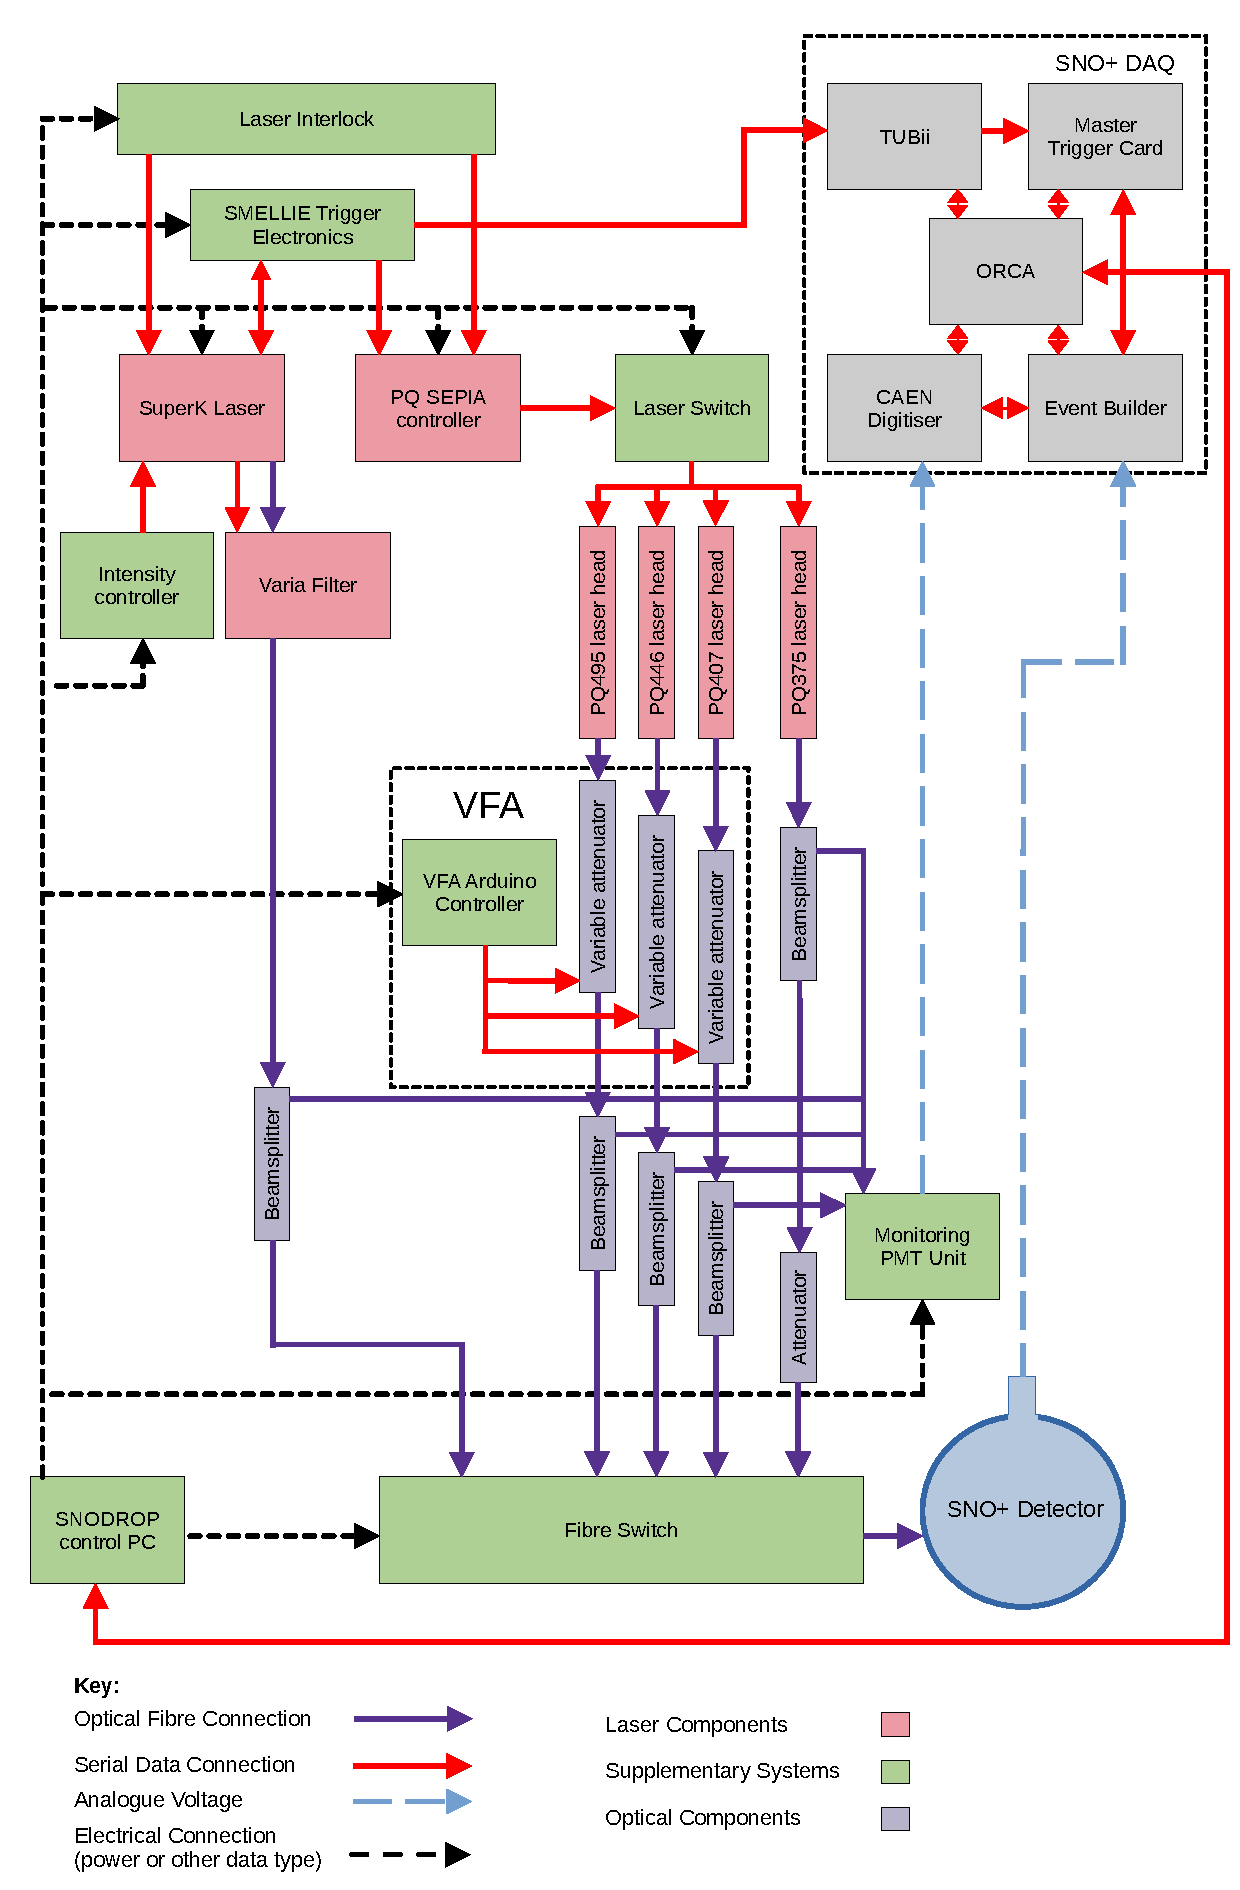
\includegraphics[width=0.95\linewidth]{3_SMELLIEHardware/images/smellie_hardware_schematic.pdf}
    \caption[Diagram of the connections between the various bits of SMELLIE hardware and the rest of the SNO+ detector]
    {Diagram of the connections between the various bits of SMELLIE hardware and the rest of the SNO+ detector, after the changes made in the Summer of 2022. Adapted from~\cite{turnerMeasurementScatteringCharacteristics2022}.}
    \label{fig:smellie_diagram_detailed}
\end{figure}

\subsection{Lasers}\label{sec:smellie_lasers}
\nomenclature{\textbf{PQ}}{PicoQuant}
Fundamental to the SMELLIE calibration system are 5 optical-wavelength lasers. Four of these are fixed-wavelength pulsed-diode laser heads from the company PicoQuant. These `PQ' laser heads each emit with a different narrow wavelength spectrum, peaking at \SI{375}{\nm}, \SI{407}{\nm}, \SI{446}{\nm}, and \SI{495}{\nm}. These are referred to as the PQ375, PQ407, PQ446, and PQ495 lasers, respectively. In addition to these lasers, a SuperK Compact laser made by NKT Photonics (hereafter referred to as the SuperK laser) is also used\footnote{
    Apologies to those more familiar with `SuperK' referring to the SuperKamiokande experiment based in Japan: this laser bears no relation.
}. Unlike the PQ laser heads, the SuperK is a super-continuum laser able to produce laser light over the whole optical wavelength spectrum. Because we are almost always interested in determining optical properties at specific wavelengths, a variable bandpass filter also built by NKT Photonics known as the SuperK Varia has been included. This allows the user to select any wavelength interval between \SIrange{400}{700}{\nm}, with a minimum bandwidth of \SI{10}{\nm}. The wavelength and emission timing characteristics of all five lasers are shown in Fig.~\ref{fig:smellie_emission_wav_timing}. The $\mathcal{O}(\SI{1}{\ns})$ time widths for the lasers are essential for scattering analyses as they allow for much greater precision in knowing when photons should arrive at PMTs in the detector than with an LED source. This is why SMELLIE uses lasers for its light generation, unlike the LEDs used for AMELLIE and TELLIE.

\begin{figure}
    \centering
    \begin{subfigure}{0.98\textwidth}
        \centering
        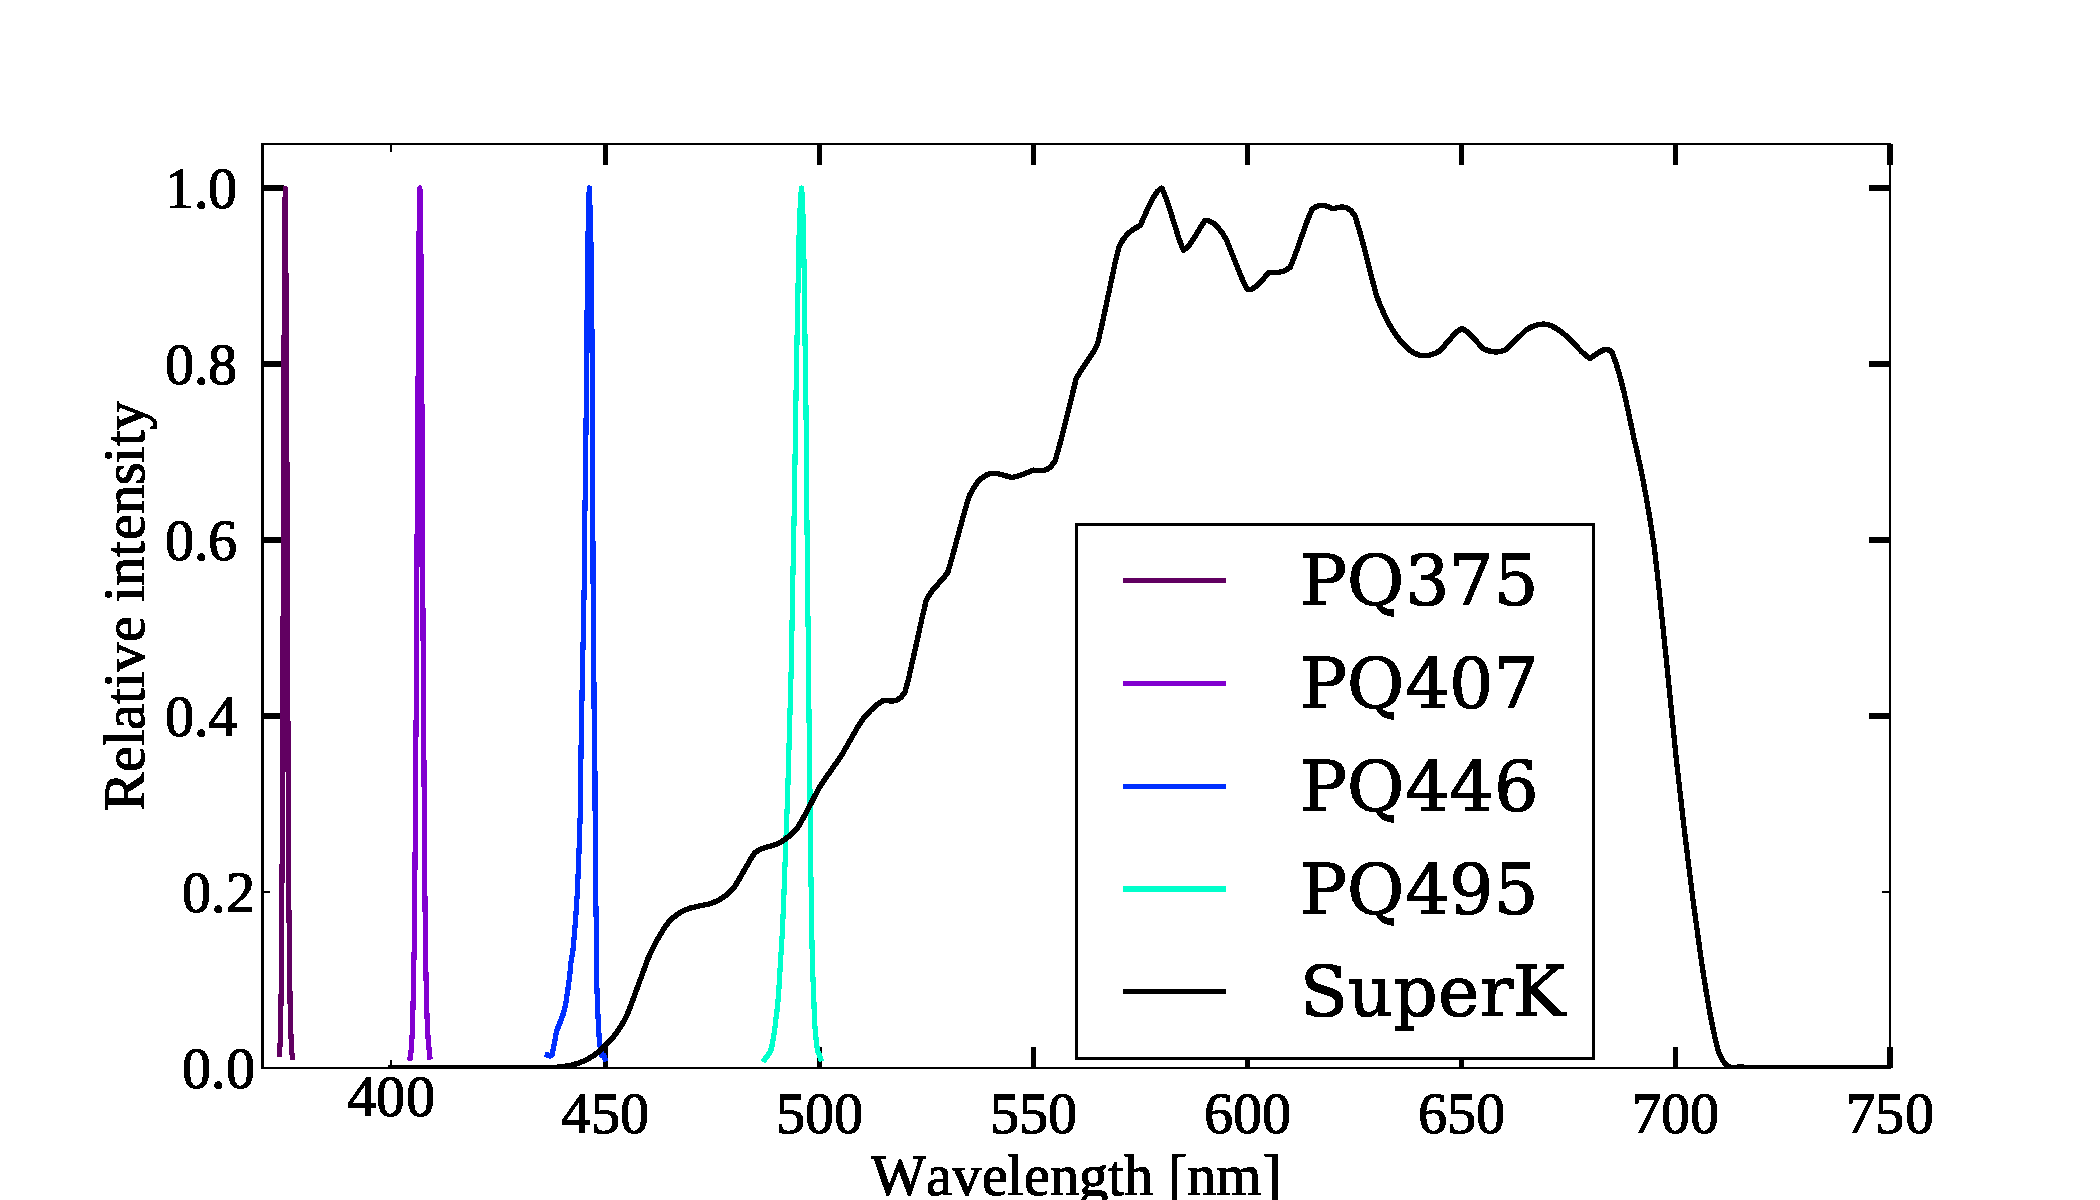
\includegraphics[width=0.98\textwidth]{3_SMELLIEHardware/images/smellie_laser_wavelengths.pdf}
        \caption{}
        \label{fig:smellie_emission_wavelengths}
    \end{subfigure}
    \begin{subfigure}{0.98\textwidth}
        \centering
        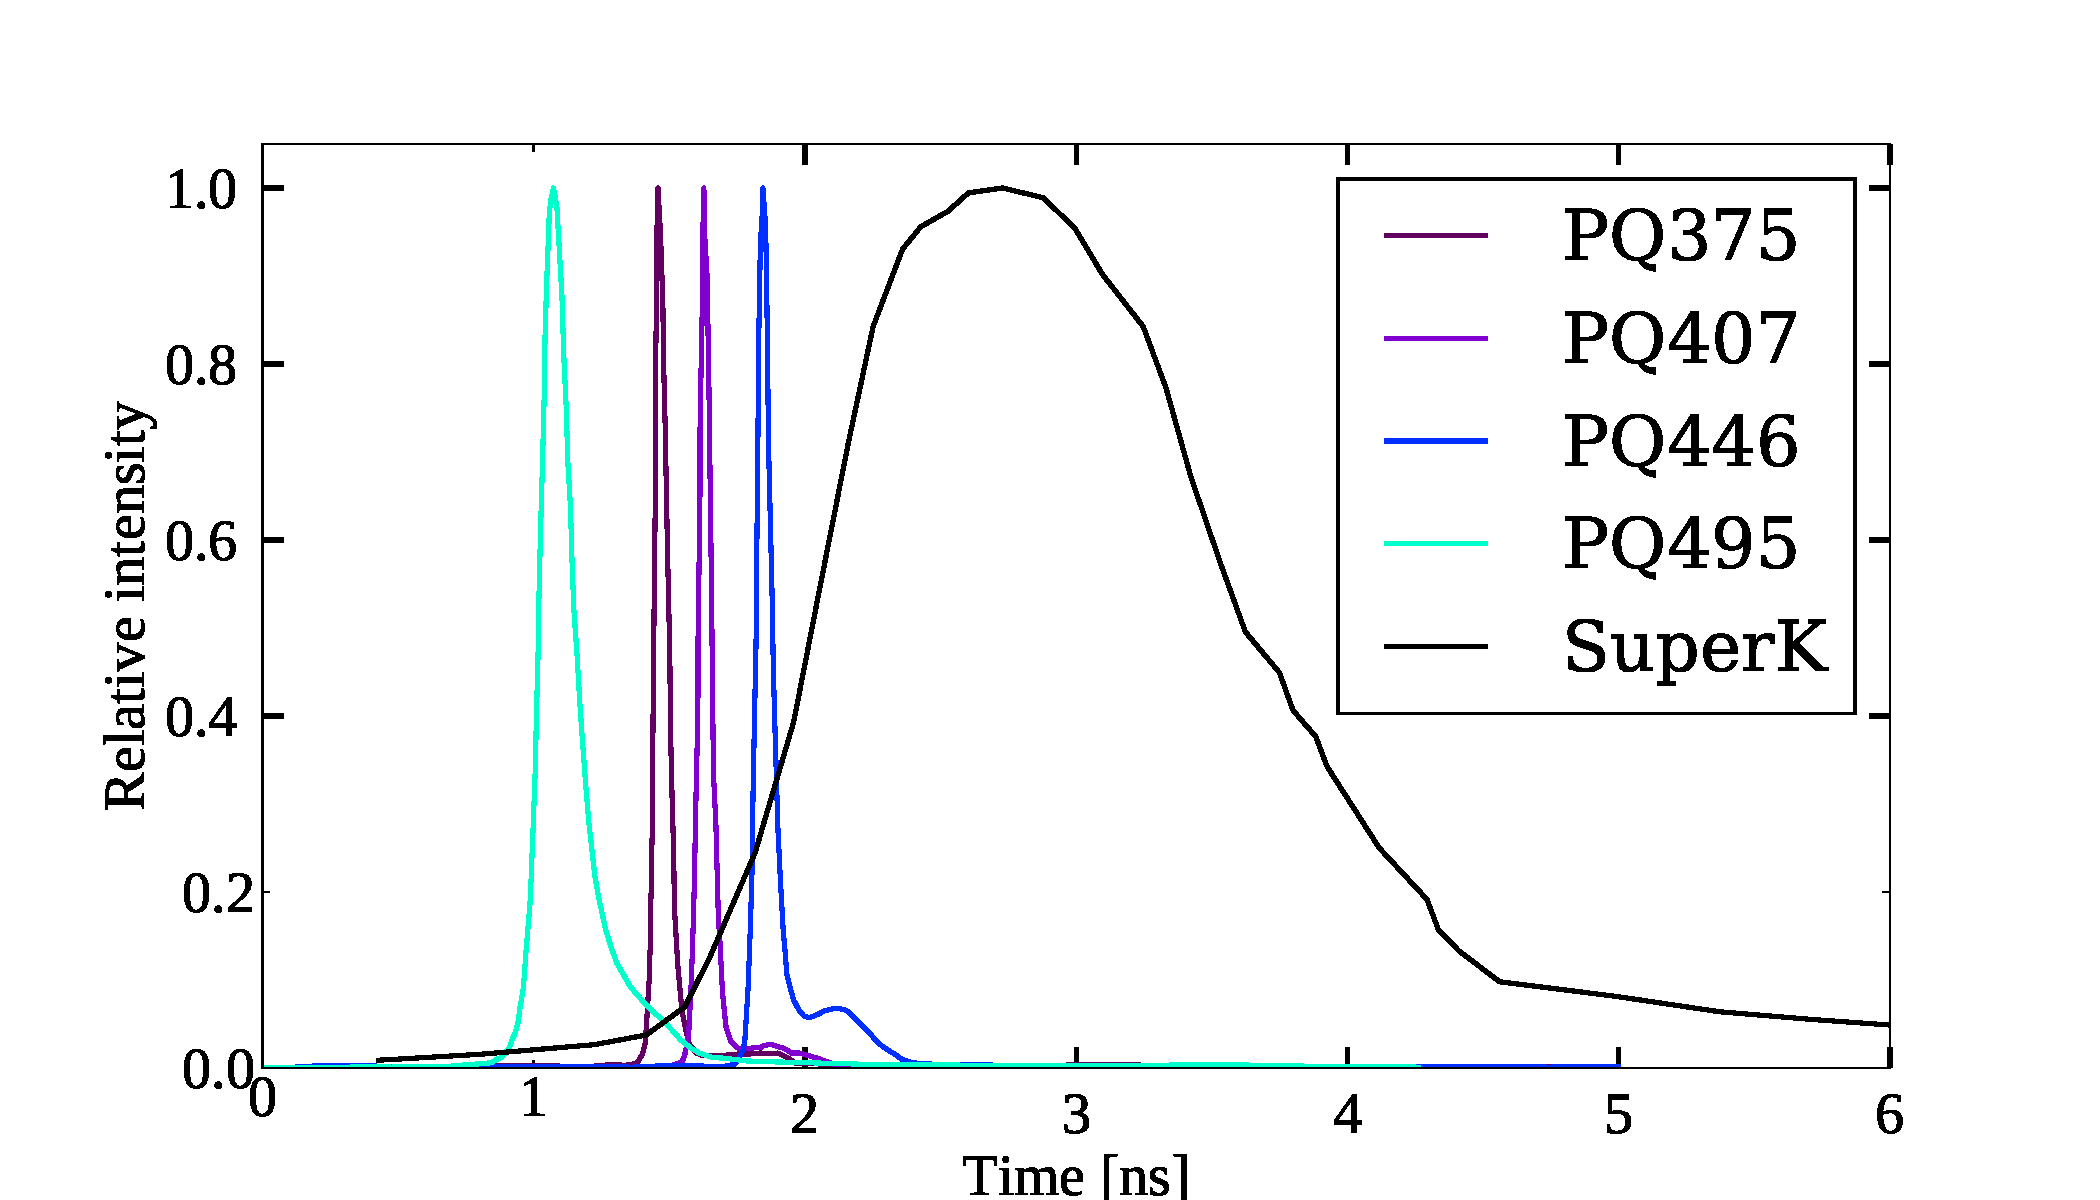
\includegraphics[width=0.98\textwidth]{3_SMELLIEHardware/images/smellie_laser_timings.pdf}
        \caption{}
        \label{fig:smellie_emission_timing}
    \end{subfigure}
    \caption[Emission wavelength and timing spectra of the lasers used in SMELLIE]
    {Emission wavelength (a) and timing (b) spectra of the lasers used in SMELLIE. PQ spectral information taken from the manufacturer~\cite{}; SuperK information measured by J. Lidgard~\cite{}.}
    \label{fig:smellie_emission_wav_timing}
\end{figure}

\subsection{Controlling Laser Intensities}\label{sec:smellie_attenuators}
It is important to be able to control the quantity of light that enters the detector from a given pulse of one of the lasers. Too much light, and because of the detector's DAQ analysis of data becomes difficult, and in the extreme case permanent damage could be done. Too little, and insufficient statistics are collected by the detector to actually do any analysis. Controlling the pulse intensity of light into the detector is done in two parts. For the SuperK laser, the raw power of the beam in a pulse can be set as a percentage of the maximum possible power for that wavelength. Once a light pulse has been generated, it is then attenuated by a neutral density filter contained within the SuperK laser hardware.

For the PQ lasers, a PicoQuant-brand SEPIA II laser driver is used to set the raw pulse intensity and firing rate. Unlike the SuperK, the intensity control is given by the laser driver's driving voltage, as a fraction of the maximum possible voltage. Problematically, the dependence on the raw output intensity of the PQ laser heads are highly nonlinear with respect to the amplitude of the driving voltage. To demonstrate, consider the observed npe per shot within the detector as a function of driving voltage for SMELLIE events using the PQ lasers: see Fig.~\ref{fig:pq_old_intensity_dependence}. For low driving voltages, the resulting npe is very small, and rises slowly. However, near a certain `lasing threshold' the npe observed increases super-exponentially, rapidly climbing many orders of magnitude in intensity. Above this threshold, increasing the driving voltage once again changes the observed intensity relatively slowly. A result of this is that if one requires an npe in the detector associated with a driving voltage that lies near the threshold, then any uncertainty in that driving voltage value can lead to dramatic changes in the npe observed. Furthermore, when driving a laser head near its lasing threshold the shot-to-shot variation in intensity can also become substantial: see Fig.~\ref{fig:pq_threshold_intensity_variation} for an example of this occurring.

\begin{figure}
    \centering
    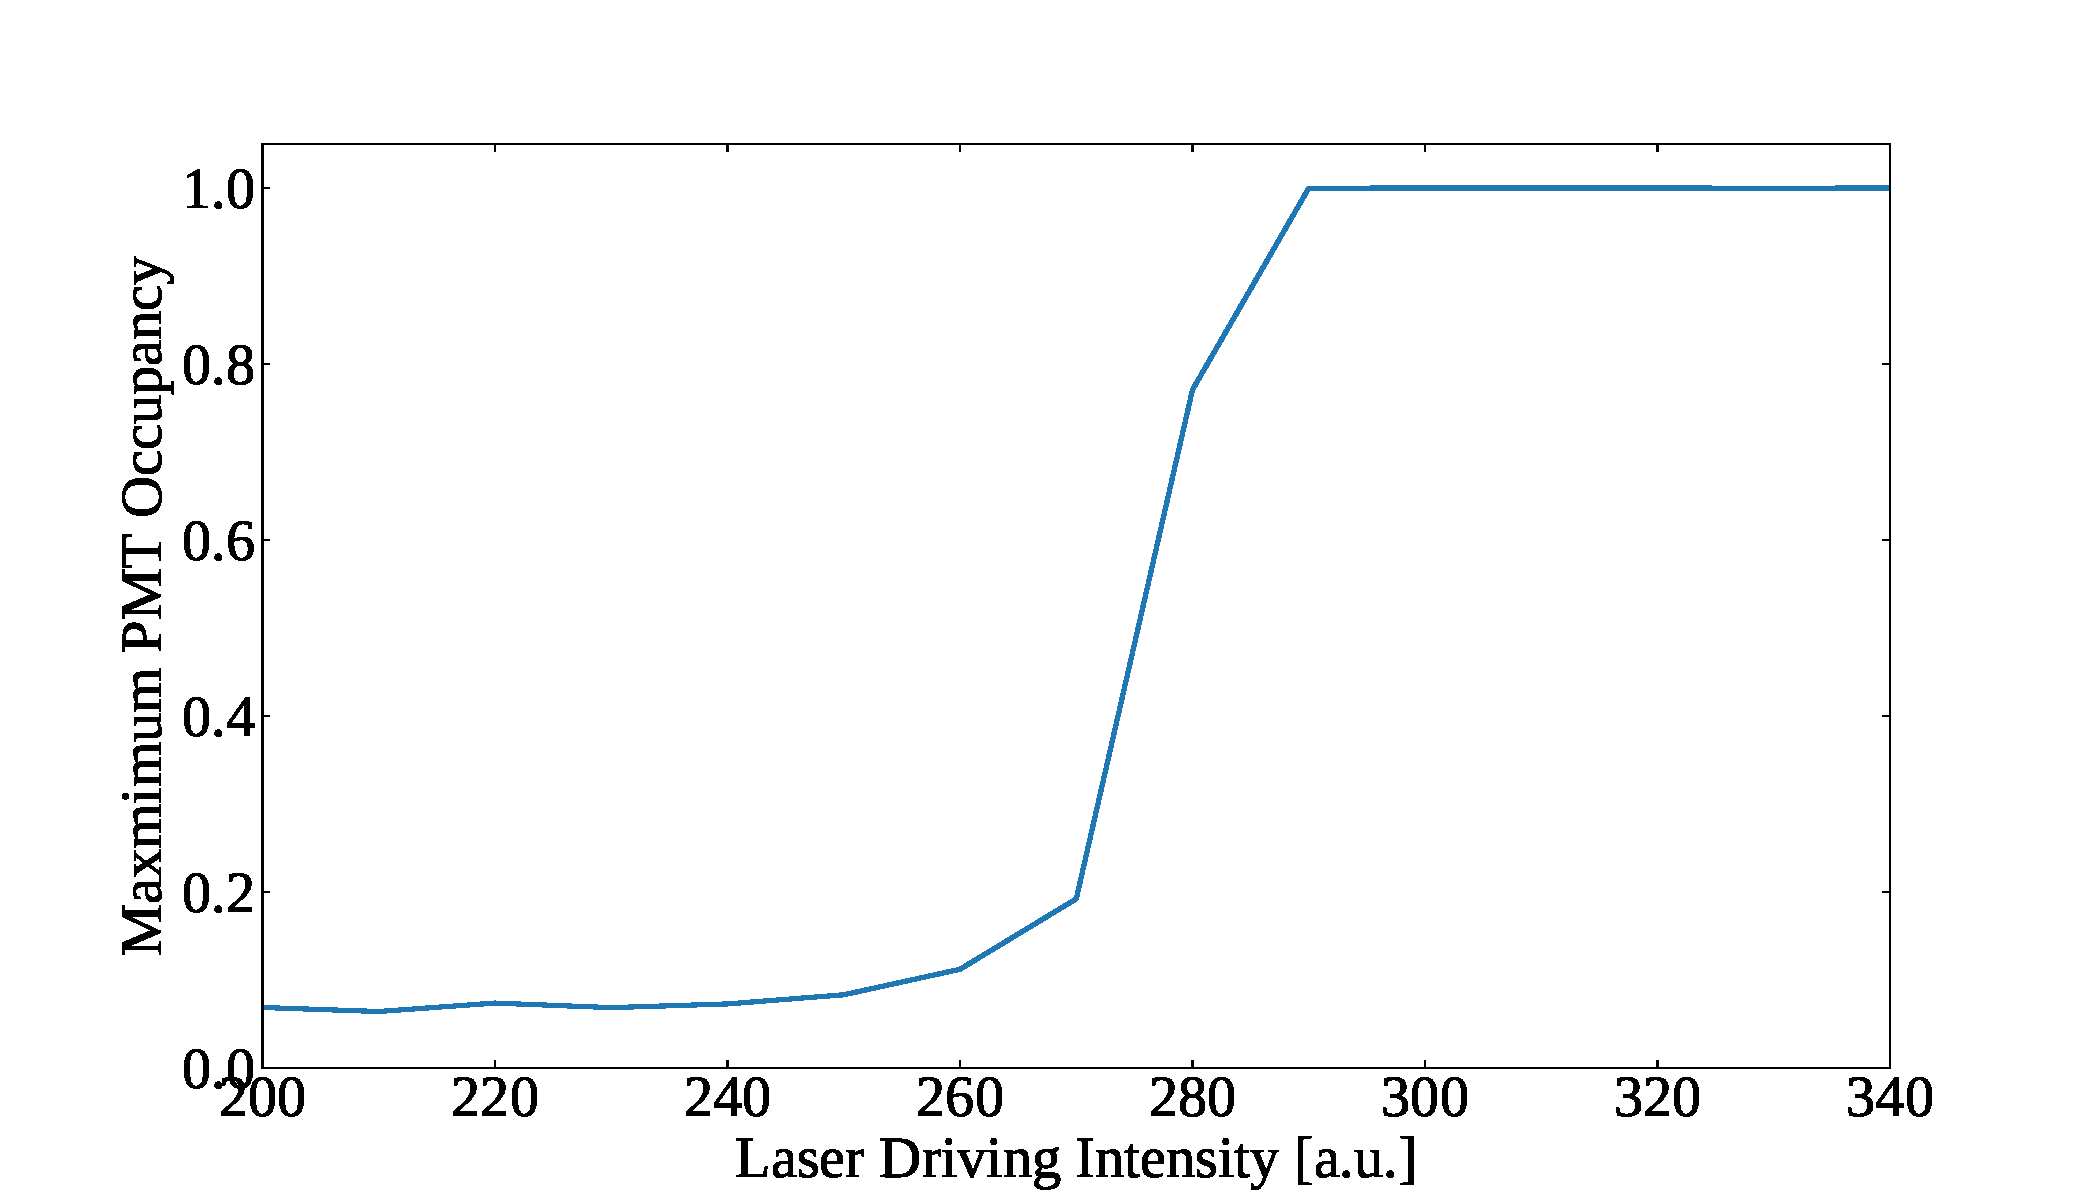
\includegraphics[width=0.8\textwidth]{3_SMELLIEHardware/images/smellie_intensity_scan_pq446_old.pdf}
    \caption[Typical impact of driving voltage intensity for PQ446 laser on observed maximum occupancy in the detector]
    {Typical impact of driving voltage intensity for PQ446 laser on observed maximum occupancy in the detector. Data taken on February 22\textsuperscript{nd}, 2021.}
    \label{fig:pq_old_intensity_dependence}
\end{figure}

\begin{figure}
    \centering
    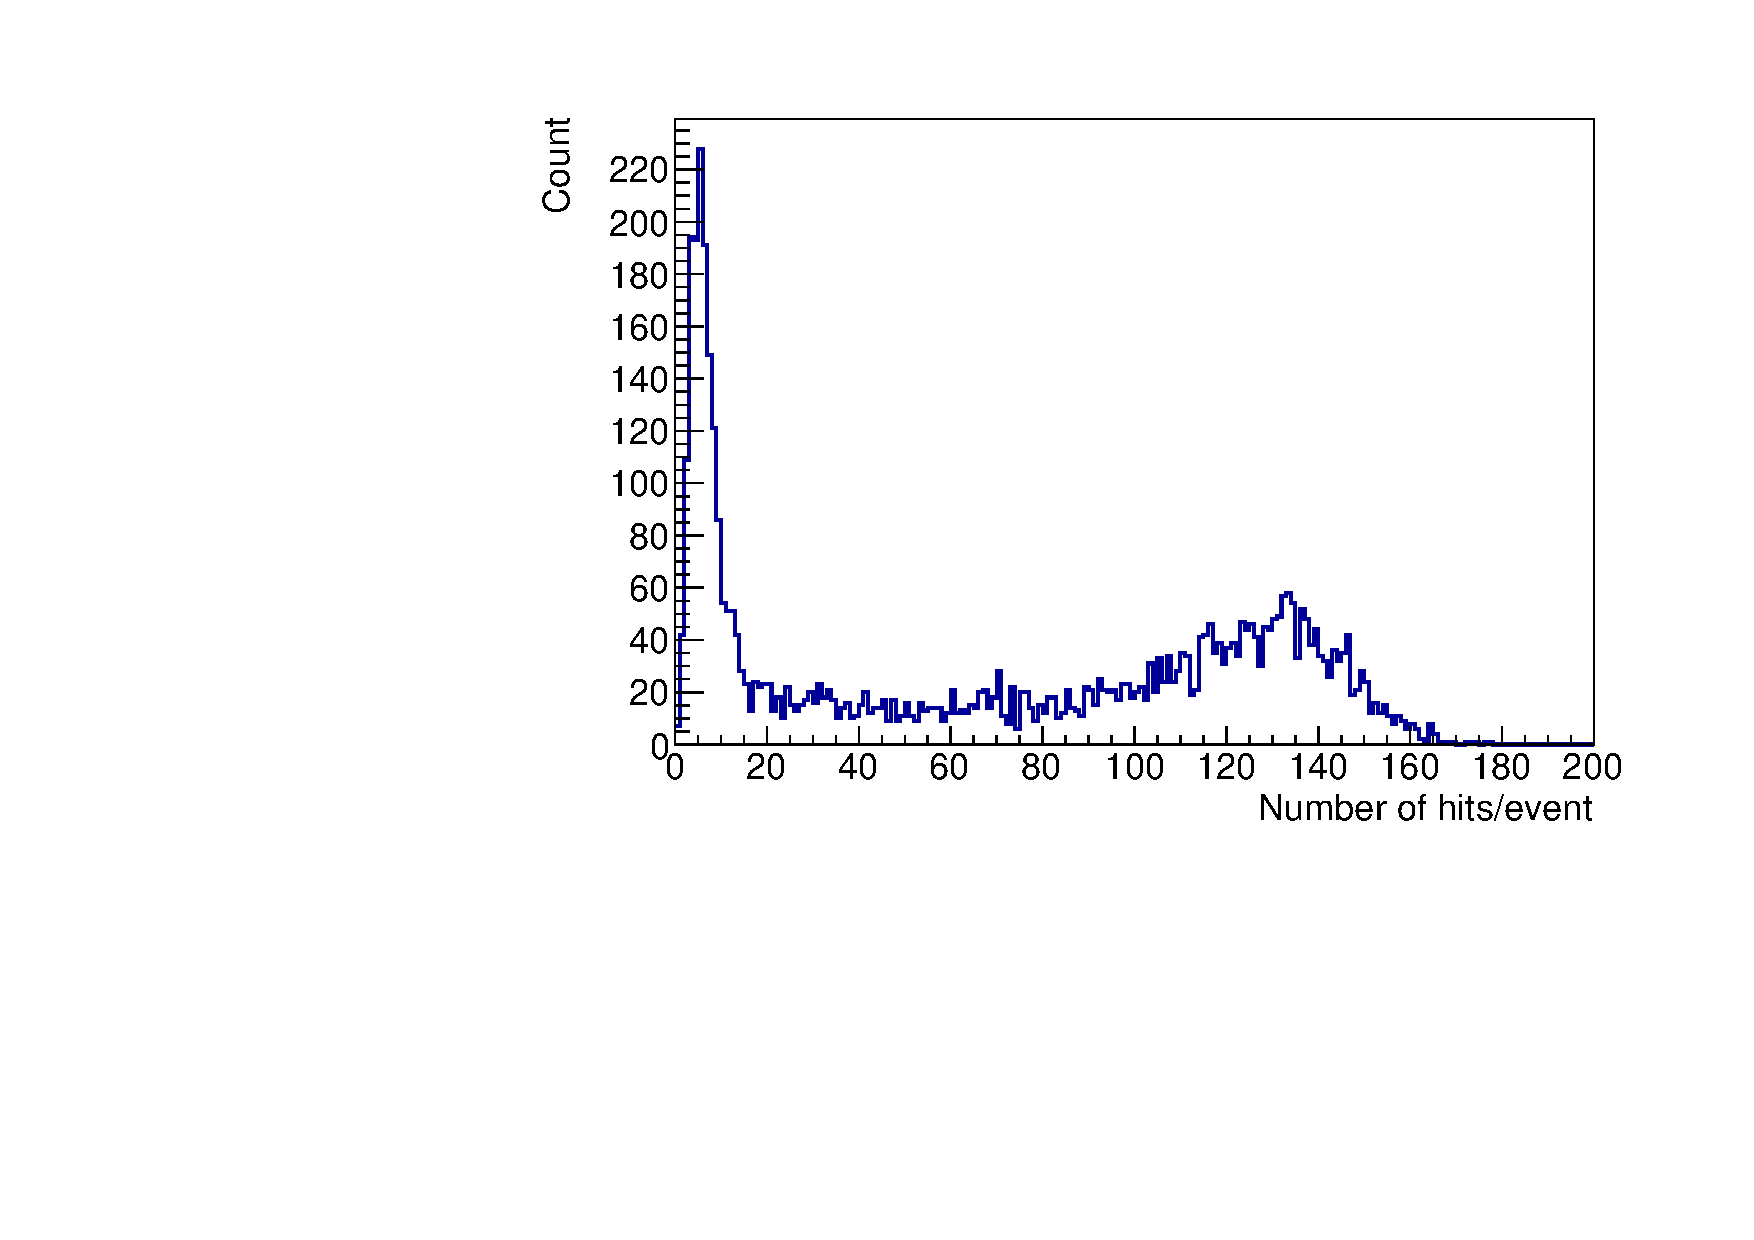
\includegraphics[width=0.8\textwidth]{3_SMELLIEHardware/images/run_268221_8_nhit_dist.pdf}
    \caption[Distribution of the number of PMT hits observed per event for laser PQ446]
    {Distribution of the number of PMT hits observed per event for laser PQ446 when the driving intensity is 280. Data taken on February 22\textsuperscript{nd}, 2021.}
    \label{fig:pq_threshold_intensity_variation}
\end{figure}

During the water phase and for much of the scintillator phase, much of the data taken, especially using the PQ407 and PQ446 lasers, suffered from large shot-to-shot intensity variations. Throughout this period, after the light was generated by a PQ laser head it would then be passed through an attenuator, fixed to some nominal attenuation setting for each laser. In theory, one could solve the intensity variation problem by deliberately setting the intensity well beyond the lasing threshold, and then changing the attenuation of the attenuator to obtain the npe within the detector one is interested in. However, under the original hardware this was untenable as this would require someone to manually change the attenuations in-person every time a different set of SMELLIE run conditions were proposed.

\nomenclature{\textbf{VFA}}{Remotely-controllable Variable Fibre Attenuator}
Instead, Jeff Lidgard built a piece of hardware called the remotely-controllable Variable Fibre Attenuator (VFA), shown in Fig.~\ref{fig:vfa_picture}. Contained within a metal housing were a `precision variable attenuator' from DiCon Fibreoptics~\cite{} % cite DiCon attenuator specsheet online
for each PQ laser, along with an Arduino running firmware written by Jeff to enable communication with each of the attenuators. Commands could be sent to a given attenuator asking for a specific attenuation between \SIrange{0}{3000}{\dB}.
Following ex-situ testing by Jeff Lidgard and Jasmine Simms, the VFA was installed underground by myself and Armin Reichold in July 2022, with some assistance from Jeff in integration of the hardware and SMELLIE server software.

\begin{figure}
    \centering
    \includegraphics[width=0.8\textwidth]{3_SMELLIEHardware/images/VFA_MPU_picture.png}
    \caption[Picture of the VFA during installation into the ELLIE hardware rack]
    {Picture of the VFA during installation into the ELLIE hardware rack. The VFA box rests beneath the fibres connecting to the beamsplitters, as well as the newly-installed Monitoring PMT Unit (see Section~\ref{sec:smellie_mpu} for details).}
    \label{fig:vfa_picture}
\end{figure}

During testing of the VFA in-situ, it was discovered that the inherent attenuation of the variable attenuator at the minimum setting of \SI{0}{\dB} for the PQ375 laser was so strong that negligible light was ever observed in the detector. Because of this, the PQ375 was not hooked up to the VFA, and kept its original attenuator setup. After fixing the driving voltage settings for PQ407, PQ446, and PQ495 to be 1000, 750, and 750 respectively, % add in numbers!
the observed npe in the detector was once again compared to the input intensity setting. For PQ375 this input parameter remained the driving voltage; for the others, the attenuation setting was now used. The results can be seen in Fig.~\ref{fig:pq_new_intensity_dependence}. As hoped for, the three PQ lasers hooked up to the VFA can now have stable intensities of light observed in the detector over multiple orders of magnitude of observed intensity.

\begin{figure}
    \centering
    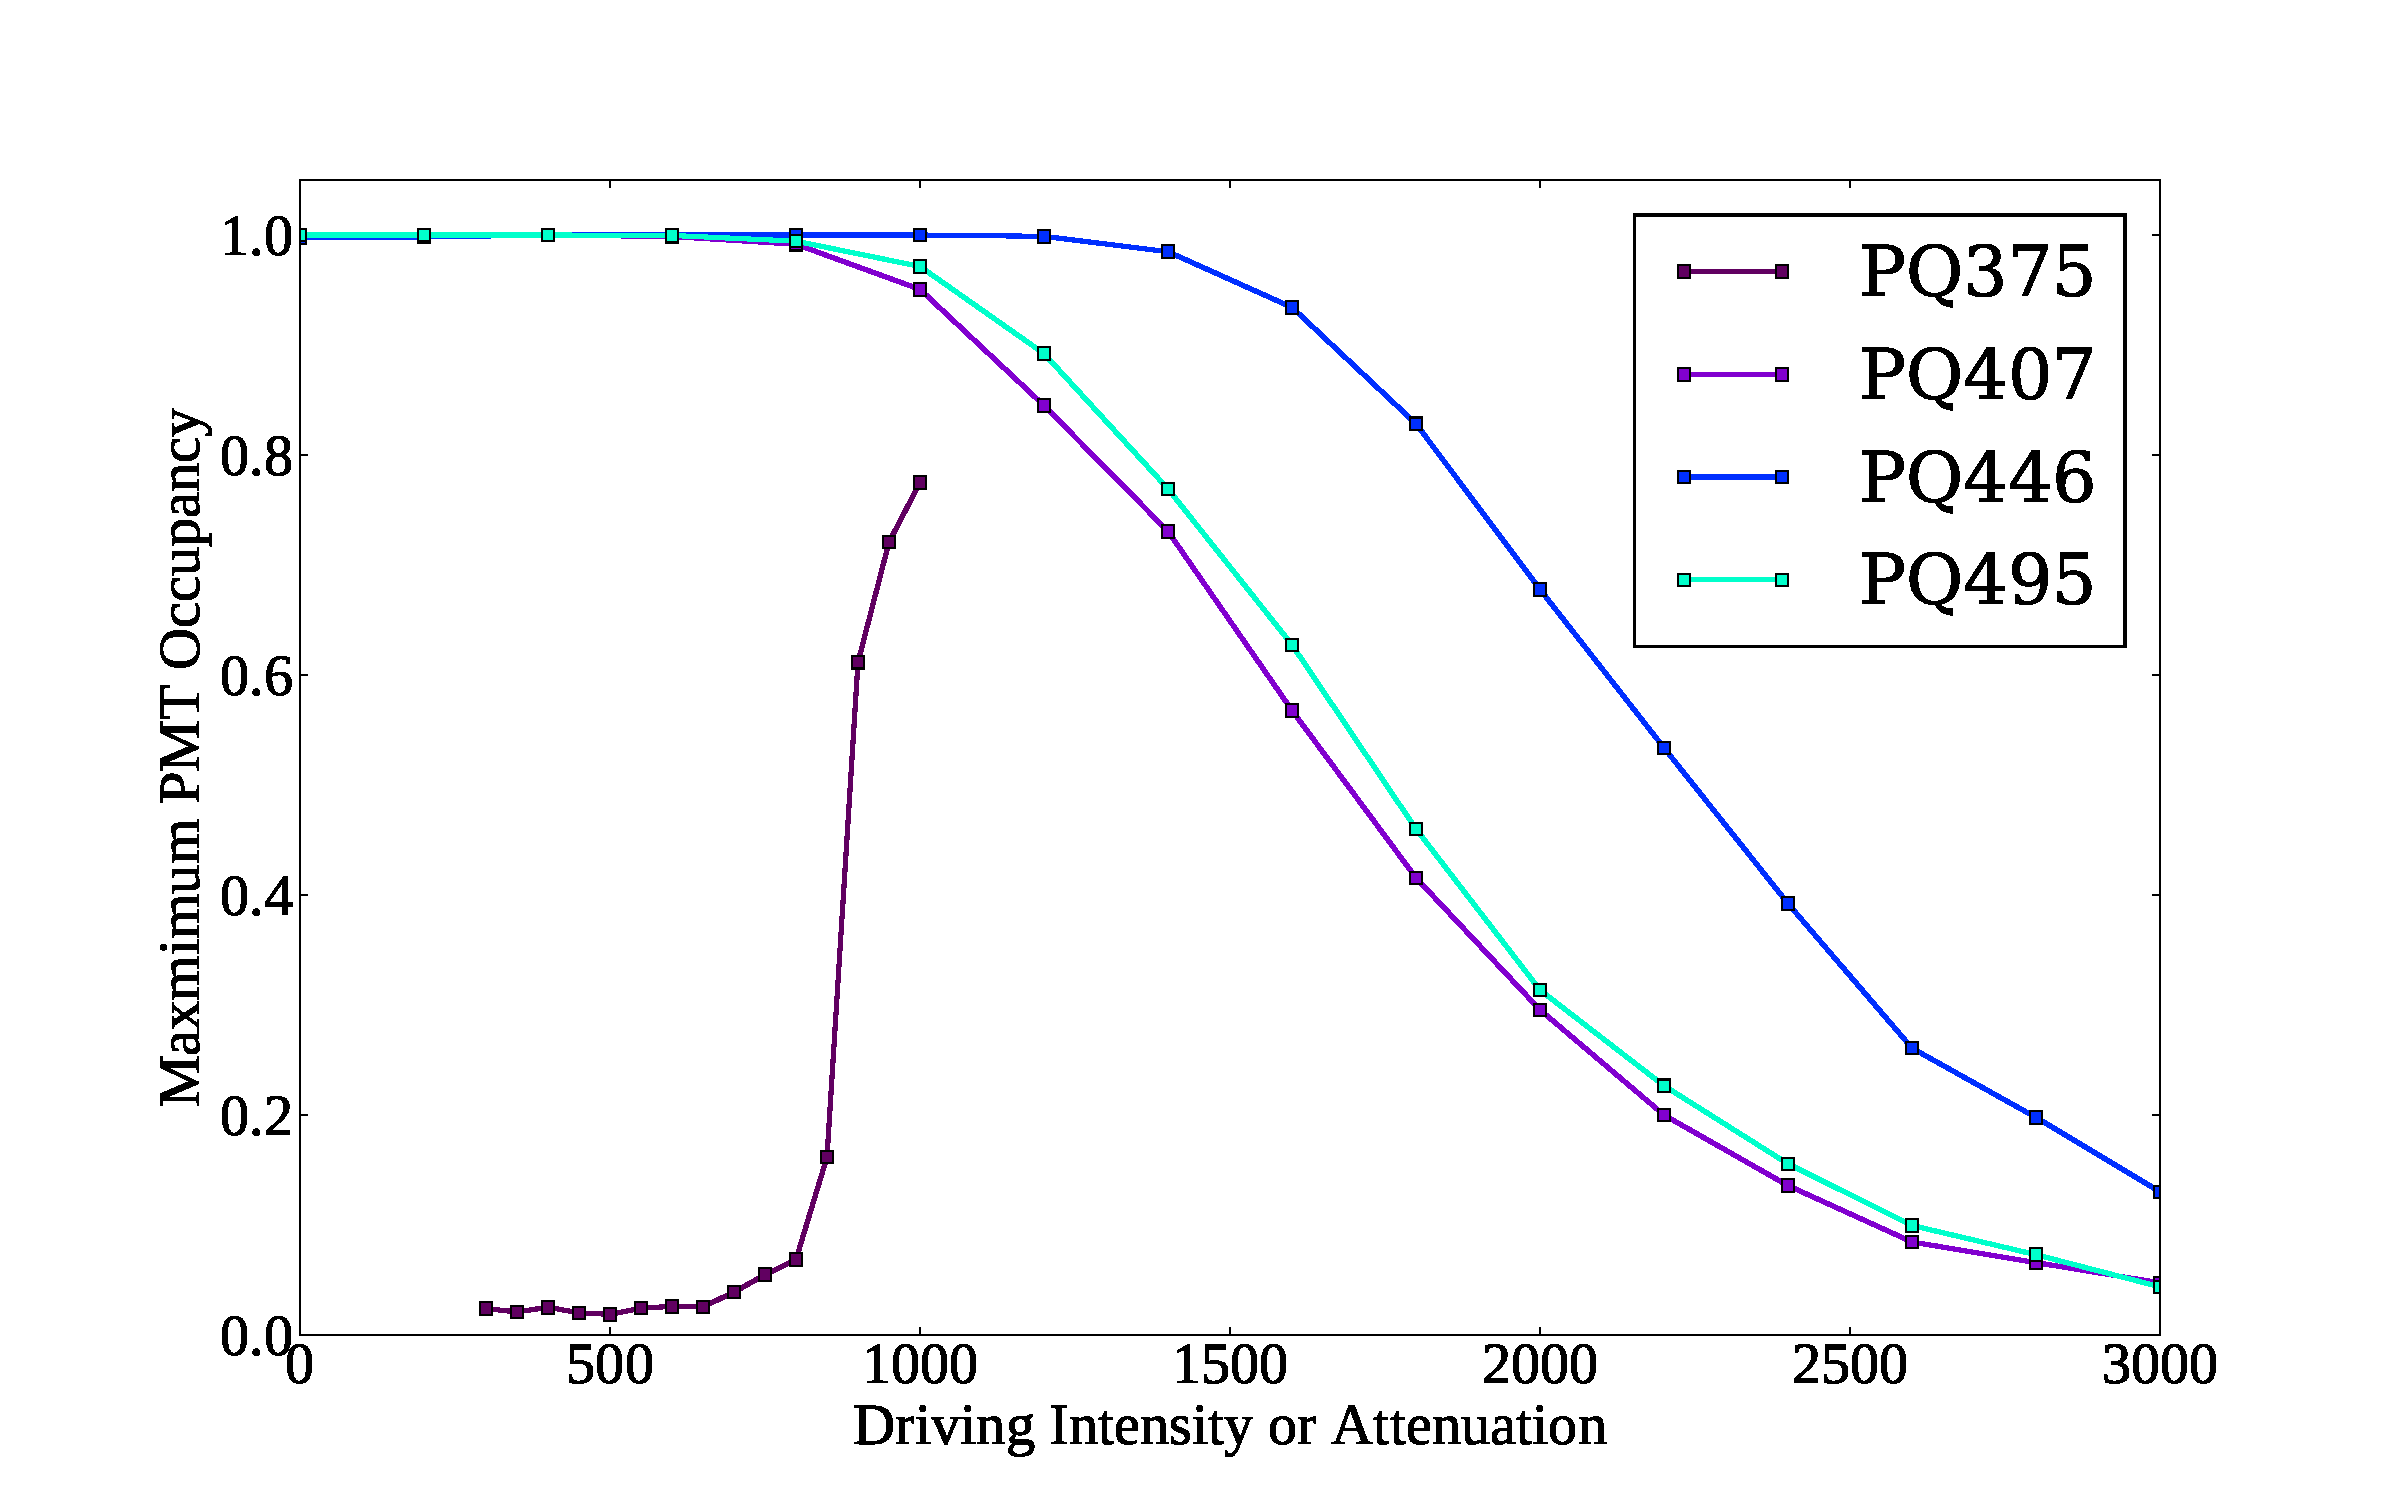
\includegraphics[width=0.8\textwidth]{3_SMELLIEHardware/images/smellie_intensity_scan_new.pdf}
    \caption[Maximum occupancy in the detector as a function of the attenuation parameter value used]
    {Maximum occupancy in the detector as a function of the attenuation parameter value used, for each of PQ407, PQ446, and PQ495. Because PQ375 is not plugged into the VFA, its dependence on the driving intensity is shown instead. Data taken on the 12\textsuperscript{th} of January, 2023.}
    \label{fig:pq_new_intensity_dependence}
\end{figure}

\subsection{Propagation of Light into the Detector}\label{sec:smellie_fibres}
Once a pulse of optical light has been generated by the lasers and attenuated to the desired intensity, the next step is to navigate that light into the detector. This is achieved through a network of Corning-brand ``InfiniCor SXi'' multimode optical fibres~\cite{}. % cite Corning datasheet(s)
These fibres were chosen in part for their low intrinsic radioactivity~\cite{}, % cite Radon Assay/Krish's thesis
as well as having a graded index as a function of radius. This latter property enables lower dispersion between different modes of the light, so that the initial sharpness of any given light pulse in time is maintained. However, because these fibres were mainly designed for telecommunication purposes, their nominal operating wavelengths are out in the near-infrared, \SIrange{750}{1450}{\nm}. As SMELLIE only fires wavelengths in the range \SIrange{375}{700}{\nm}, there is a small but non-negligible amount of light lost when propagating through the fibres.

After some light is split off by a beamsplitter to allow for ex-situ monitoring of the light pulse (see Section~\ref{sec:smellie_mpu}), it is sent to the Fibre Switch, two boxes manufactured by Laser Components UK~\cite{} % cite Laser Components UK
that allows a user to remotely-control which of the fibres to send the light down into the detector.

Finally, the light that passes through the fibre switch propagates along one of the 15 optical fibres that have been submerged in the SNO+ cavity, whose ends are mounted to the PSUP. Specifically, sets of three fibres are mounted to a given node of the PSUP, with associated node numberings: nominally 07, 25, 37, 55, and 21. These provide for a variety of positions within the detector from which light can be emitted. Each mounting which holds three of the optical fibres also contains collimators, designed to reduce the possible range of angles with which the light can be emitted from. This is particularly important for SMELLIE, because unlike the other ELLIE systems, a thin `pencil' beam of light across the detector is ideal for measuring scattering~\cite{majumdarMeasurementOpticalScattering2015}. % cite Krish.
One last thing the mounting achieves is to point each of the three fibres in different directions: \ang{0}, \ang{10}, and \ang{20} from the direction radially towards the centre of the detector.

Each fibre is given a name that nominally refers to both its mounting position and its pointing direction. For example, the label `FS107' corresponds to the SMELLIE fibre mounted at node 07 with a pointing direction of \ang{10}. Unfortunately, during installation some fibres were mislabelled, leading to the node mounting points and pointing directions of some fibres being inconsistent with the labelling convention. The actual pointing directions for each fibre can be seen in Table~\ref{tab:smellie_fibre_labellings}.
The 3D positions and pointing directions of all the fibres are shown in Fig.~\ref{fig:smellie_pos_dirs}.

\begin{table}
    \centering
    \begin{tabular}{c c c}
        \hline
        Fibre   & Node & Pointing direction \\ \hline \hline
        FS007   & 07   & \ang{0}  \\
        FS107   & 07   & \ang{10} \\
        FS207   & 07   & \ang{20} \\
        FS025   & 25   & \ang{0}  \\
        FS125   & 25   & \ang{10} \\
        FS225   & 25   & \ang{20} \\
        FS037   & 37   & \ang{10} \\
        FS137   & 37   & \ang{0}  \\
        FS237   & 37   & \ang{20} \\
        FS055   & 55   & \ang{10} \\
        FS155   & 55   & \ang{20} \\
        FS255   & 55   & \ang{0}  \\
        FS093   & 21   & \ang{0}  \\
        FS193   & 21   & \ang{10} \\
        FS293   & 21   & \ang{20} \\
        \hline
    \end{tabular}
    \caption[SMELLIE fibre names, their associated mounting nodes on the PSUP, and their pointing direction.]
    {SMELLIE fibre names, their associated mounting nodes on the PSUP, and their pointing direction. Taken from~\cite{turnerMeasurementScatteringCharacteristics2022}.}
    \label{tab:smellie_fibre_labellings}
\end{table}

\begin{figure}
    \centering
    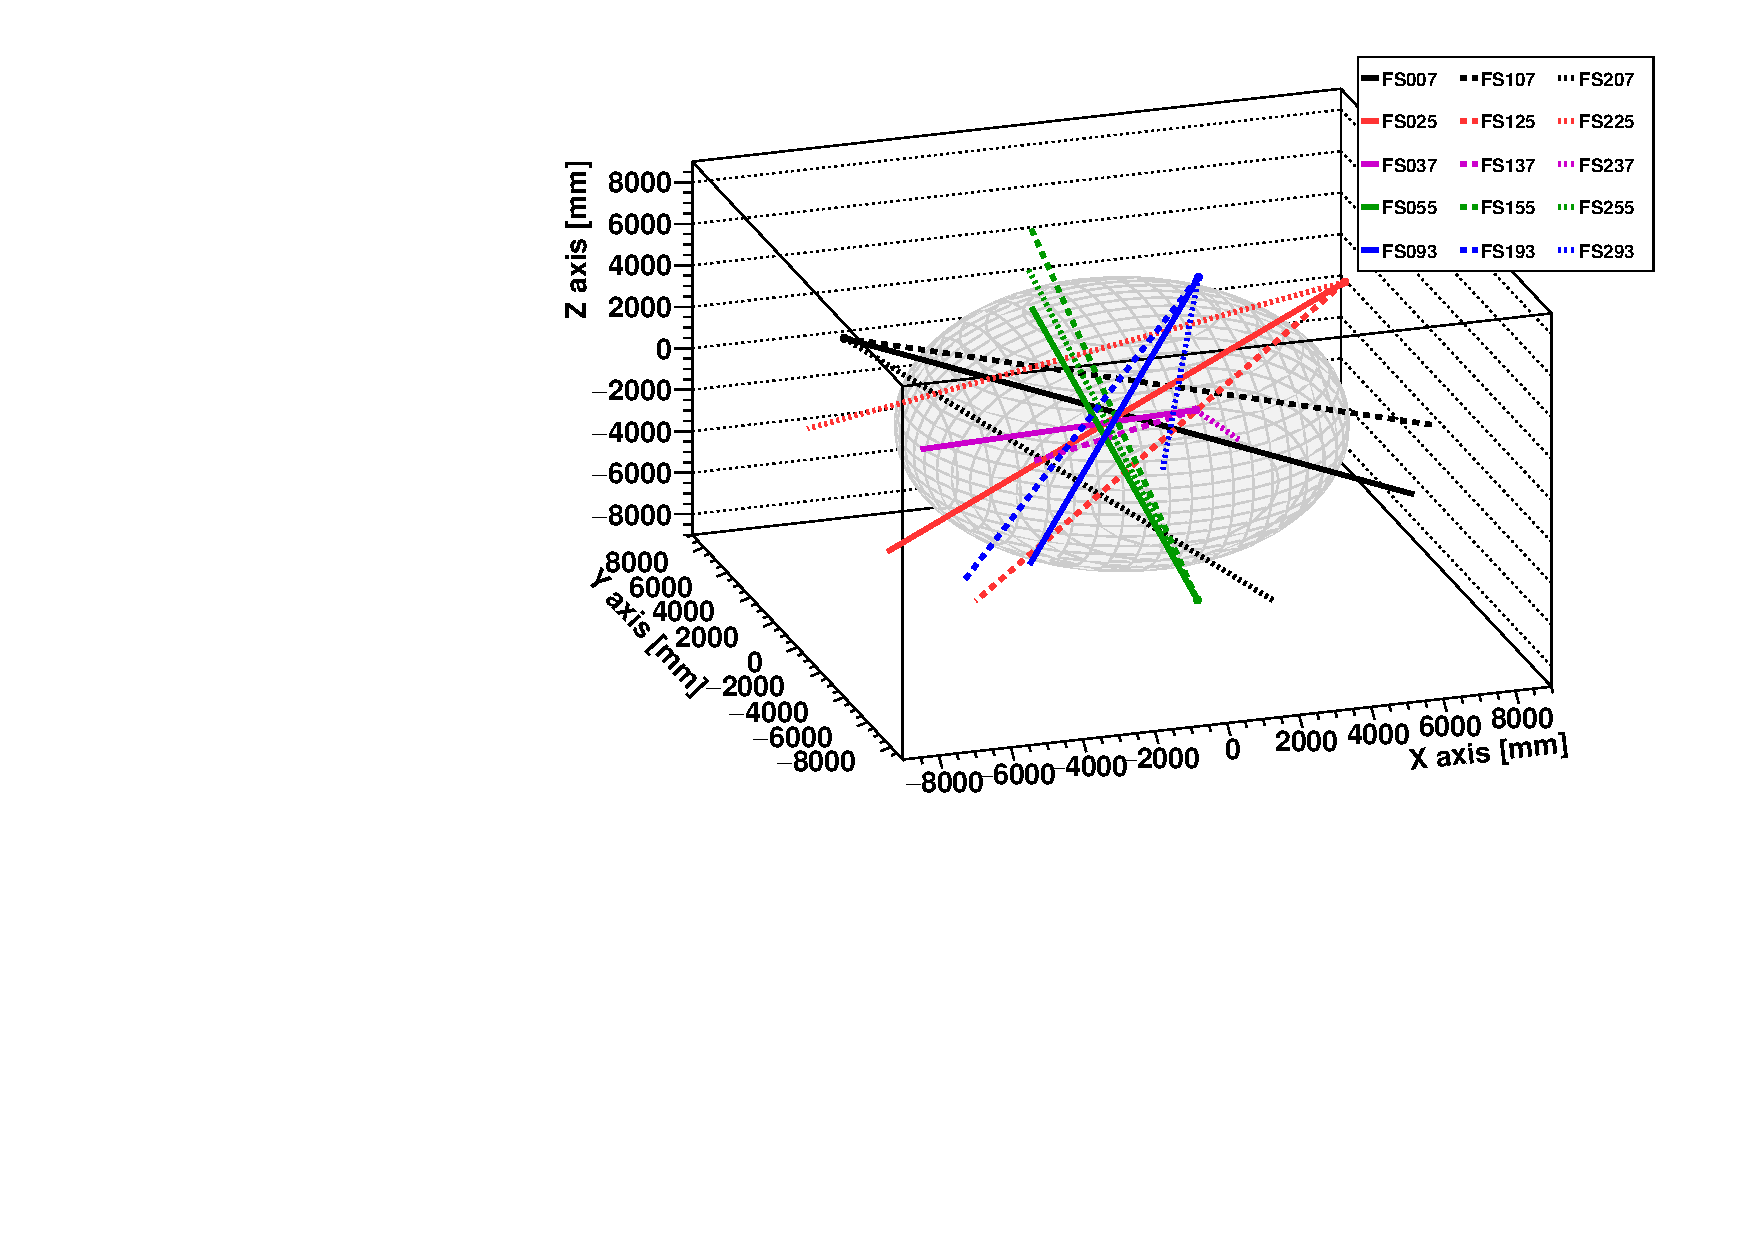
\includegraphics[width=0.8\textwidth]{3_SMELLIEHardware/images/fibre_positions.pdf}
    \caption[Fibre emission points and nominal pointing directions]
    {Fibre emission points and nominal pointing directions within the detector.}
    \label{fig:smellie_pos_dirs}
\end{figure}

When performing analysis with SMELLIE, a fibre-centric spherical-polar coordinate system is used for clarity. This coordinate system was first fully-developed by E. Turner; full details can be read in~\cite{turnerMeasurementScatteringCharacteristics2022}. A position $\bm{x}$ is measured relative to a given fibre's mounting position, $\bm{f}$ (hereafter referred to as simply the fibre's position). Polar angles, labelled $\alpha$, are measured relative to the fibre's nominal pointing direction, $\bm{\hat{u}}$. As a result, a line from the fibre position along $\alpha = 0$ across the detector should in theory hit the centre of the fibre's beamspot. Finally, in order to define the azimuthal angle $\phi$, the plane orthogonal to $\bm{\hat{u}}$ is considered. Both $\bm{x}$ and the unit vector in the vertically-upwards direction, $\bm{\hat{z}}$, are projected onto this plane, forming the vectors $\bm{x_{proj}}$ and $\bm{\hat{z}_{proj}}$, respectively. $\phi$ is then defined as the angle going from $\bm{\hat{z}_{proj}}$ to $\bm{x_{proj}}$ if one were to look at the plane in the direction of $\bm{\hat{u}}$. Mathematically, this can be written as:
\begin{equation}
    \tan\phi = \frac{
        \left(\bm{x_{proj}}\times\bm{\hat{z}_{proj}}\right)\cdot\bm{\hat{u}}
        }{\bm{x_{proj}}\cdot\bm{\hat{z}_{proj}}}.
\end{equation}

\subsection{The Monitoring PMT Unit}\label{sec:smellie_mpu}
\nomenclature{\textbf{MPU}}{Monitoring PMT Unit (for SMELLIE)}
As mentioned in the previous section, part of the light generated by the lasers gets split off from the main fibre path down into the detector, and instead is used for monitoring purposes. This is achieved with a box known as the Monitoring PMT Unit (MPU). As the name suggests, the MPU contains a small PMT that generates an electronic signal pulse from the laser light. This signal is then shaped by electronics, and passed to the detector's central CAEN digitiser to have that pulse digitised.

One problem with the existing MPU within SMELLIE was that the pulse it produced was so broad that 300 ADC samples were needed to capture the full shape (the CAEN samples at a rate of 1 every \SI{4}{\ns}). This led to a large fraction of data being generated by SMELLIE events coming not from the PMT hit information, but simply the MPU's signal digitisation. A natural consequence of this was the rate at which the lasers could be fired had to be limited to typically \SI{1}{\kHz}, otherwise the detector was not able to handle the rate of data being generated.

Because of this, a new MPU was commissioned. Built by Adam Baird and Johan Fopma from the Oxford Physics Central Electronics Group, this MPU had updated electronics such that the pulse was shaped shorter. In addition, the rise time of the pulse was made faster, in the hopes that the emission time of the light pulse for a given event could be captured more accurately. The new MPU was installed by myself and Armin Reichold at the same time as the VFA, in Summer 2022.

Alongside the installation of the new hardware, the settings in ORCA for the CAEN digitisation of the MPU signal were updated. In particular, the number of samples made by the CAEN was shortened from 300 down to 124. The timing of the CAEN sampling and delay on the TUBii trigger (more on the trigger shortly) was also modified. As a result of these changes, the shortest possible trace was now being generated, without missing any part of the MPU pulse or moving the observed TAC for hits in the detector outside the trigger window. Fig.~\ref{fig:caen_trace_comparison} shows a comparison between typical MPU pulses taken before and after the upgrades.

\begin{figure}
    \centering
    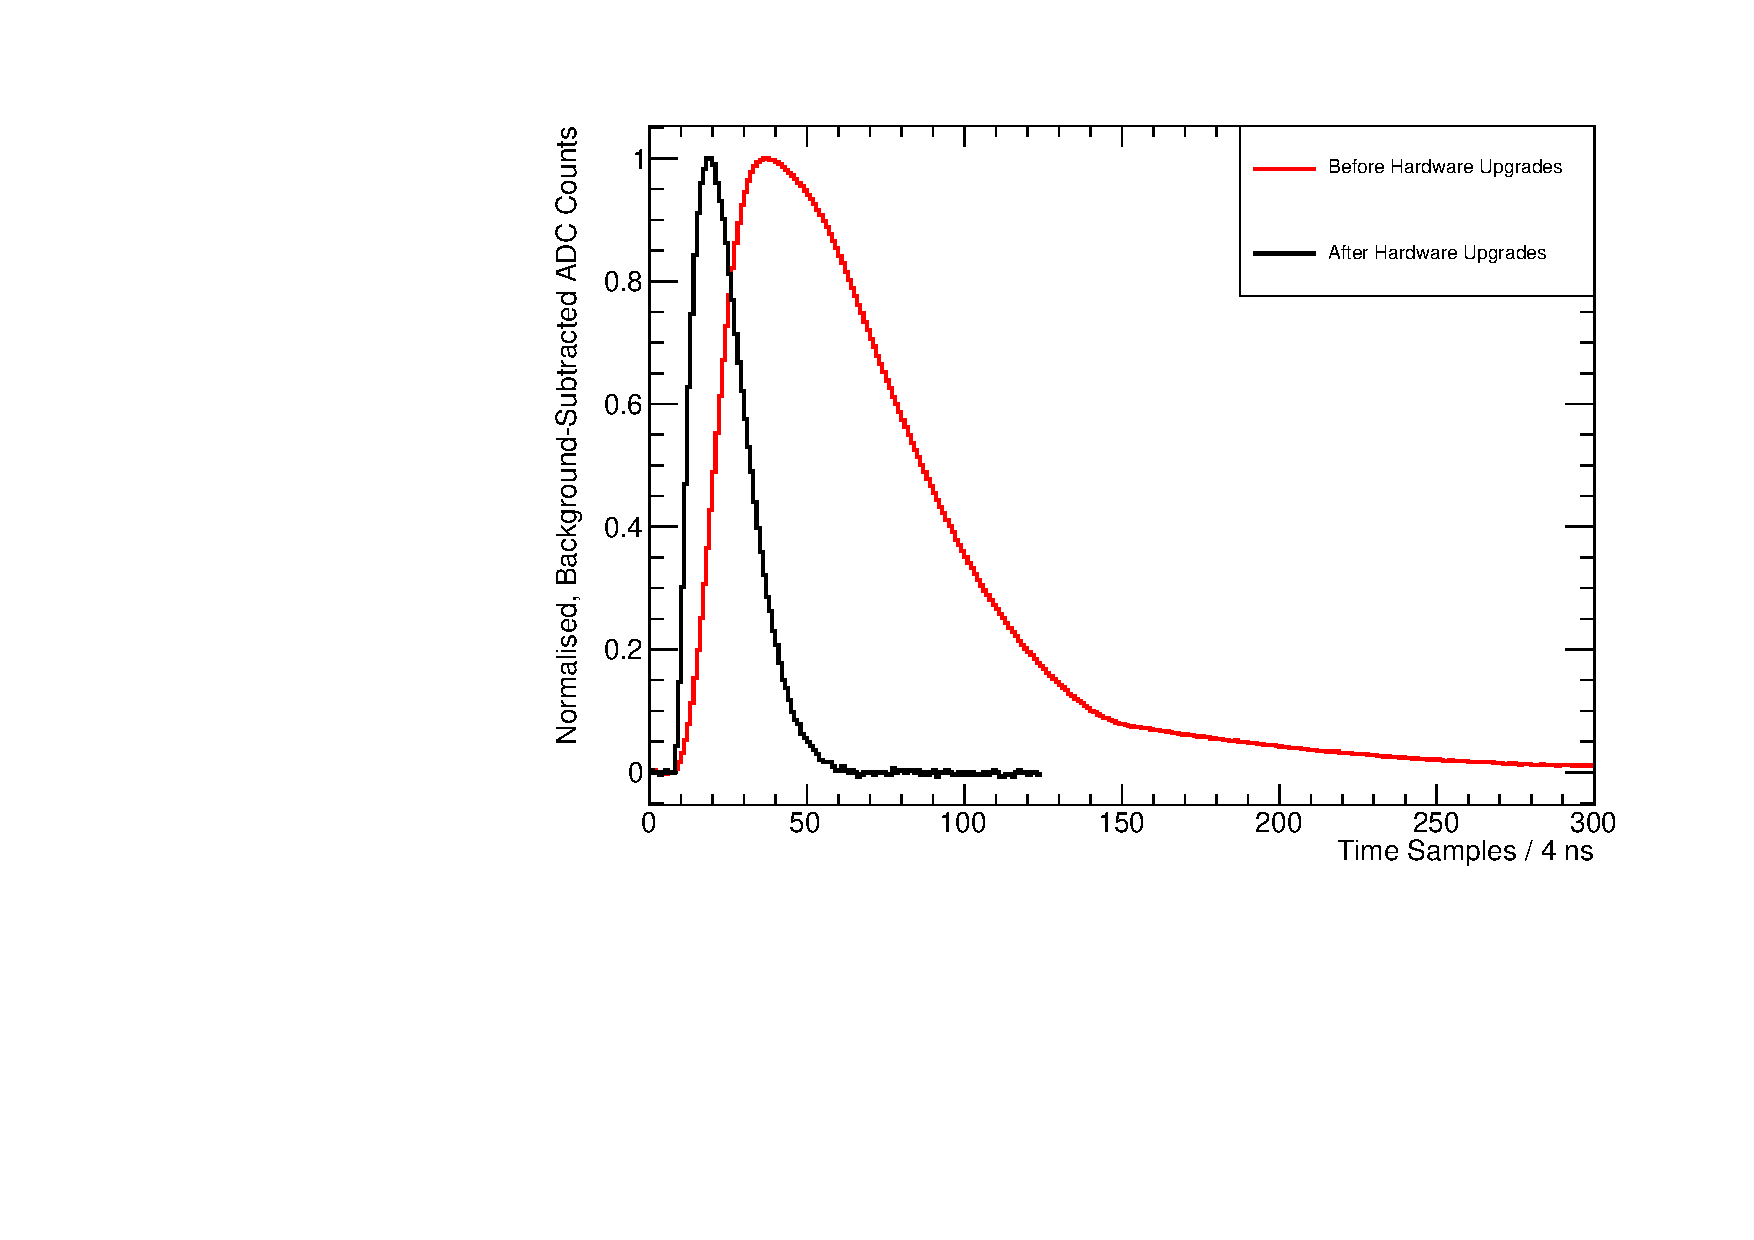
\includegraphics[width=0.8\textwidth]{3_SMELLIEHardware/images/caen_traces_comparison_plot.pdf}
    \caption[Comparison between typical MPU CAEN traces generated by the PQ495 before and after the Summer 2022 hardware upgrades]
    {Comparison between typical MPU CAEN traces generated by the PQ495 before and after the Summer 2022 hardware upgrades. The data before was taken on July 24\textsuperscript{th} 2022, whilst the data after was taken on June 17\textsuperscript{th} 2023. The traces have had their baselines subtracted off, and their peak values normalised to 1.}
    \label{fig:caen_trace_comparison}
\end{figure}

\subsection{Event Triggering and Data Acquisition}\label{sec:smellie_triggering_daq}
As mentioned in Section~\ref{sec:daq}, it is possible to trigger the SNO+ detector electronics via an external asynchronous trigger, EXTA. Taking data with SMELLIE takes advantage of this capability: instead of waiting for the normal `physics' triggers such as N100 to pick up the event, because we know when we are firing the laser we can send an EXTA signal to trigger the detector precisely when a light pulse is within the detector.

\nomenclature{\textbf{NI Unit}}{National Instruments DAQ Unit (for SMELLIE)}
Trigger signal pulses are created by the National Instruments DAQ Unit (the `NI Unit'), in place alongside the rest of the SMELLIE electronics. These trigger pulses are sent to either the PQ's SEPIA controller or the SuperK laser to induce the firing of the relevant laser. If a PQ laser was fired, a trigger pulse is simultaneously sent to TUBii, which after a delay sends an EXTA trigger signal to the MTC/D, which then issues a GT. In contrast, the SuperK has a substantial variation in the emission time of laser light relative to a given driving pulse. Instead of sending the trigger signal to TUBii in parallel to the SuperK laser, a photodiode contained within the SuperK laser system is able to detect any generated light, and from that detection a new trigger signal is sent to TUBii.

A major problem with the handling of the trigger signal delay by TUBii was present throughout the collection of water phase SMELLIE data. This delay was `latched' to the \SI{100}{\MHz} clock present within the electronics of TUBii. As a result, the observed hit times of PMTs in the detector (which are relative to the GT time) was a convolution of the hit times without the latching and a top hat function of width \SI{10}{\ns}.

An example of this effect in action can be seen in Fig.~\ref{fig:smellie_beam_tres_tubii_comparison}. Light from the PQ495 laser was fired through fibre FS007 by E. Turner in June 2018, during the water phase. Looking only at PMTs that were hit in the beamspot, defined here as PMTs with $\alpha<\ang{3}$, the trigger times can be fit to the convolution of a Gaussian with a \SI{10}{\ns} top hat.

\begin{figure}
    \centering
    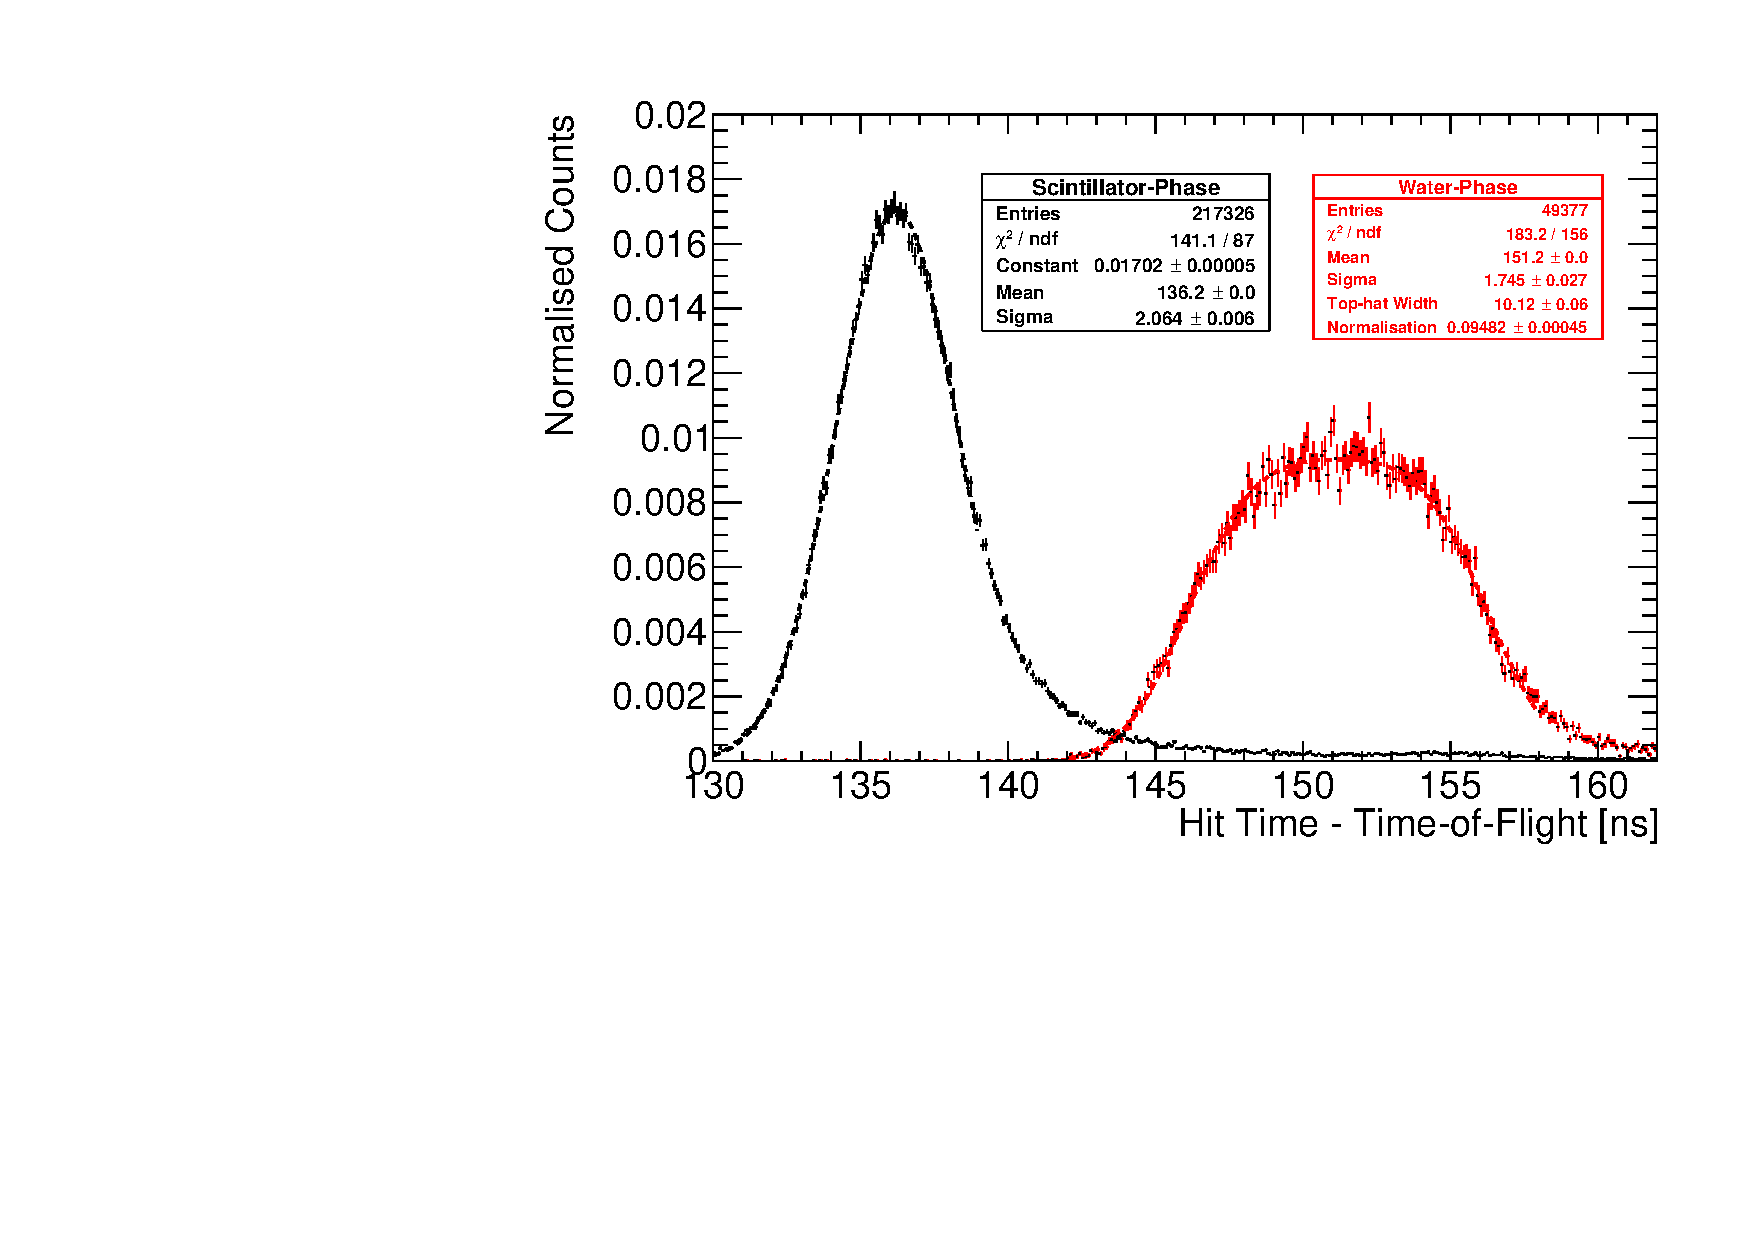
\includegraphics[width=0.8\textwidth]{3_SMELLIEHardware/images/time_plots_comparison_114018_vs_302634_FS007_nice.pdf}
    \caption[Comparison of observed hit times in beamspot before and after TUBii firmware update]
    {Comparison of observed hit times in beamspot for laser PQ495 through fibre FS007, before and after T. Zummo's firmware update to TUBii. The initial data was taken by E. Turner June 20\textsuperscript{th} 2018 during the water phase, whilst the data post-fix was taken by myself on July 24\textsuperscript{th} 2023 during the scintillator phase. The peak of the former is fit to the convolution of a Gaussian with a top-hat function, whilst the latter is just fit with a Gaussian function.}
    \label{fig:smellie_beam_tres_tubii_comparison}
\end{figure}

During the partial fill phase, Tony Zummo updated the firmware of TUBii so that this latching would no longer occur, and the arrival times to the MTC/D were truly asynchronous to any clocks. The results are also shown in Fig.~\ref{fig:smellie_beam_tres_tubii_comparison}: notice how the width of the peak is now much sharper. This width is determined by the TTS of the hit PMTs, with the width of the PQ495 timing pulse being a subdominant effect.

Because this fix to TUBii was not in place until after all water phase data taking had been completed, any analysis of SMELLIE data from the water phase had to contend with this \SI{10}{\ns} trigger `jitter'. Fortunately, this jitter was global to all hit times of a given event, so if measured a correction could be made.

In this thesis, two similar approaches are used to measure the event-by-event emission time $t_{\mathrm{emm}}$, the time at which laser light first emanates from the fibre in a given event. In both, the calibrated hit times of PMTs within the beamspot $t_{\mathrm{hit}}$ have the time-of-flight of light travelling from the fibre to the given PMT, $t_{\mathrm{TOF}}$ subtracted. $t_{\mathrm{TOF}}$ is calculated by using the ``Light Path Calculator'' algorithm developed within \texttt{RAT}. In one method, used both within the analysis work of E. Turner~\cite{turnerMeasurementScatteringCharacteristics2022} % cite anyone else?
and in Chapter~\ref{chap:beam_profiling} of this thesis, $t_{\mathrm{emm}}$ is measured as the second-earliest value of $t_{\mathrm{hit}}-t_{\mathrm{TOF}}$ in the beamspot. This method, called the ``$t_{\mathrm{emm}} = t_{2}$'' approach, skips the earliest event in the beamspot to be robust to noise hits.

Alternatively, in the ``$t_{\mathrm{emm}} = t_{\mathrm{med}}$'' approach, the median value of $t_{\mathrm{hit}}-t_{\mathrm{TOF}}$ in the beamspot is used. We shall see in Chapter~\ref{chap:smellie_analysis} that using $t_{2}$ has a bias as a function of the number of hits in the beamspot in a given event, whereas $t_{\mathrm{med}}$ does not.

This event-by-event approach to reconstructing $t_{\mathrm{emm}}$ is only necessary when the trigger system has unresolved problems. Because of the fix to the TUBii firmware, data taken using the PQ lasers during the scintillator phase did not in theory require using either of the $t_{\mathrm{emm}}$ reconstruction methods described above. However, for the SuperK laser a new problem was made clear. In Fig.~\ref{fig:smellie_superk_double_peaks} one can see the hit times of beamspot PMTs for SuperK light of wavelengths in the interval $[490,500]\;\si{\nm}$ from fibre FS125, taken on June 17\textsuperscript{th} 2023. % COMPLETE!
A clear double-peaked structure can be seen. Also shown on the plot is the distribution of $t_{2}$ values. If the laser light were being emitted in two pulses for a given event, then we would expect to see only one bump in this distribution. However, the shape of the $t_{2}$ is clearly bimodal in a manner matching that of the overall timing distribution: this indicates that the actual emission times of light from the fibre can come at two different times relative to the GT time.

\begin{figure}
    \centering
    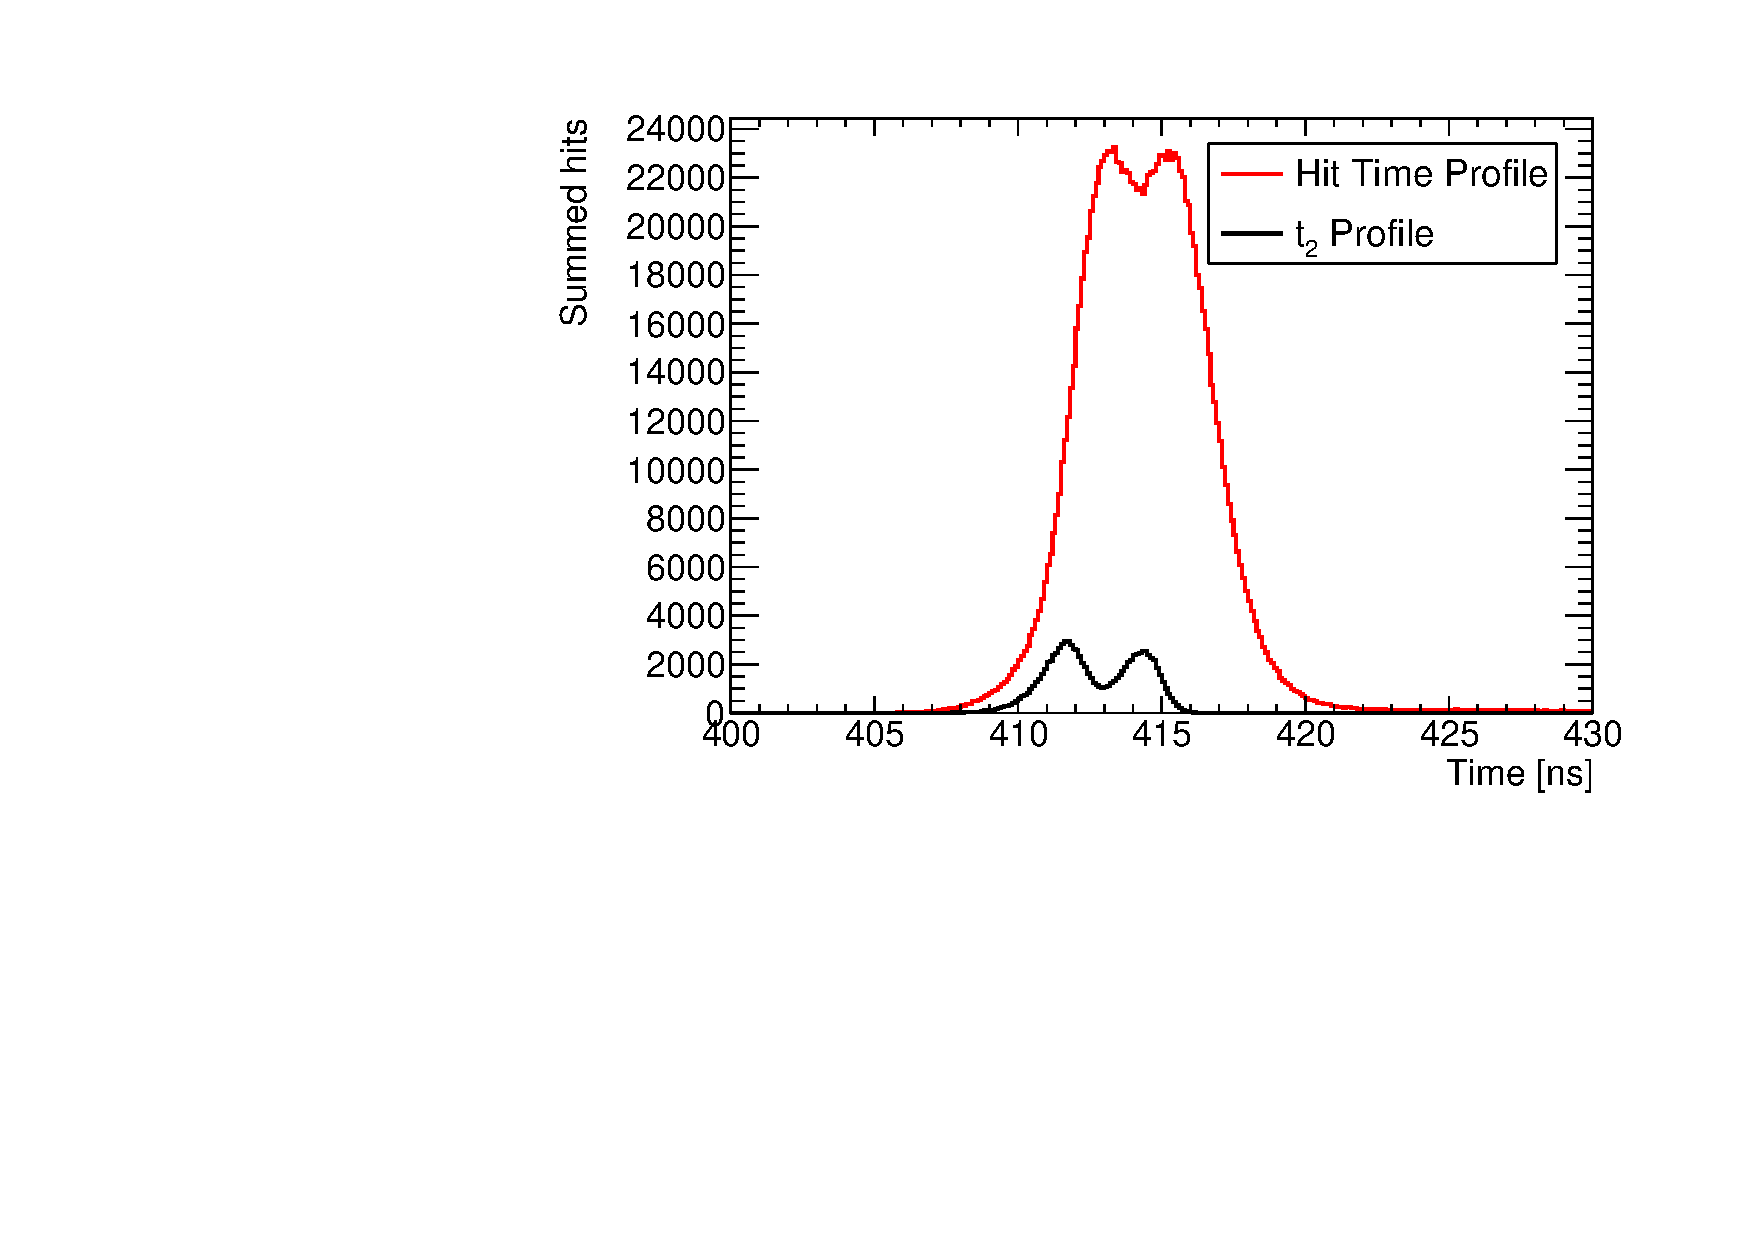
\includegraphics[width=0.8\textwidth]{3_SMELLIEHardware/images/time_t2_plot_310303_SK495_FS125.pdf}
    \caption[]{Hit time and $t_{2}$ distributions for a subrun of SMELLIE data taken with the SuperK laser in the $[490,500]\;\si{\nm}$ range through fibre FS125 on June 17\textsuperscript{th} 2023. The double-peaked structure is clear in both distributions.}
    \label{fig:smellie_superk_double_peaks}
\end{figure}

The origin of this double-peaked structure for SuperK events remains unresolved. However, the fact that events from the PQ lasers do not see this effect indicates that the issue likely lies somewhere in the part of the triggering system unique to the SuperK laser. For work within this thesis, it was decided to continue to use an event-by-event approach to $t_{\mathrm{emm}}$ for data from all phases and lasers, to ensure consistency.

% TALK ABOUT PULSEGT????

% \begin{itemize}
%     \item Describe the existing hardware, post-upgrade made in Summer 2022. For pre-upgrade hardware, can simply cite previous SMELLIE theses. This includes the path of light into the detector, as well as the path of the trigger signal.
%     \item Make sure to mention explicitly these upgrades: Tony Zummo's fix to the TUBii trigger logic, as well as the addition of the VFA, updated MPU, and modified trigger window. Make sure to motivate why these updates were made.
% \end{itemize}
% [7 pages]
\section{Software for SMELLIE Data-taking}
The process of taking data with SMELLIE is largely automated. The user begins by deciding on the settings --- the number of laser pulses and their frequency, as well as which fibre, laser, wavelength, intensity, and attenuation (if relevant) --- that will be used for each subrun. One run of SMELLIE data taking can have an arbitrary number of subruns within it, each with their own setting. This is organised into a ``run plan'' \texttt{JSON} file for that run, and uploaded to a central CouchDB server for storage.

To begin data taking, ORCA is used to put the DAQ into a `SMELLIE' run type, which disables almost all the usual `Physics' triggers such as N100 and N20. The only triggers still masked into the MTC/D are:
\begin{itemize}
    \item EXTA: This is obviously needed to capture the trigger signals sent from SMELLIE.
    \item ESUMHI: This residual physics trigger is kept in with a high threshold, to capture any high-\texttt{nhit} events not coming from SMELLIE, e.g. if a supernova were to go off whilst SMELLIE data taking was occurring.
    \item PULSEGT: This is a special trigger that fires at a rate of \SI{50}{\Hz} independent of all other systems. Using this trigger the noise rate can be calculated on a run-by-run basis for each channel.
\end{itemize}
The noise rates derived from the PULSEGT triggers are automatically calculated during the processing of runs, and are stored in \texttt{RATDB} tables. As mentioned in Section~\ref{sec:ev_simulation}, \texttt{RAT} can use these tables to replicate the noise levels in each PMT when generating simulations to match data. When performing analysis on SMELLIE data, only events from an EXTA trigger are usually considered.

With ORCA, one can then load in any run plan already uploaded to the CouchDB server, and then execute it. ORCA then sends commands describing the instructions laid out in the run plan to a server running on a computer called SNODROP, which is housed in the same pair of electronic racks as the rest of the SMELLIE hardware. This server converts these high-level commands into the low level instructions understood by the specific pieces of SMELLIE hardware needed to actually send the correct number of pulses of laser light of the right wavelength and intensity through the correct fibre.

Whilst SMELLIE data is being taken, a ``run description'' \texttt{JSON} file is generated and then uploaded to the SMELLIE CouchDB server, describing the settings of the SMELLIE run actually executed. This differs from the run plan slightly in two main ways: firstly, the same run plan can be run on multiple occasions. However, a run description file is associated to exactly one run of data that was actually taken. Secondly, if a SMELLIE run was terminated early either by the detector operator, or from a hardware problem, the run description file will correctly show only the subruns that were actually performed. The code repository used in all SMELLIE analysis has been updated by myself to use a given run description file in concert with the associated SMELLIE data file, so that the subrun-level metadata can be known during analysis.


% \begin{itemize}
%     \item Can be brief here! Little has changed since previous theses, so can mostly just summarise and cite.
%     \item Server running on SNODROP machine, which converts high-level commands into low-level ones that the hardware can interpret.
%     \item Run plan files written in JSON handed to ORCA which then sends relevant commands to SNODROP which fires as appropriate.
%     \item Operator interacts with ORCA to perform SMELLIE calibration runs.
%     \item After SMELLIE data taken, run description file created, containing metadata about the run conditions, used in analysis.
% \end{itemize}
% [2 pages]

% MAYBE DO NOT INCLUDE SMELLIE COMMISSIONING SECTION????

% \section[Commissioning SMELLIE in the Scintillator Phase]{Commissioning SMELLIE in the\\ Scintillator Phase}

% {
% \color{blue}
% \begin{itemize}
%     \item Explain why commissioning of SMELLIE is needed: Need to confirm that SMELLIE is working as expected; determine intensity "set-points" for different use cases.
%     \item Commissioning originally performed by Esther and JeffL back in the water phase; explain why this needed to be re-done for both the scintillator phase and after the hardware upgrades.
%     \item No need to describe the Tesseract in detail here - that can be in Jeff L's thesis. But, I do want to show the results of both commissioning campaigns in scintillator-fill, one before the new hardware was added, and one after.
% \end{itemize}
% [5 pages]
% [15 PAGES TOTAL]
% }
\chapter{Simulating SMELLIE Events}\label{chap:beam_profiling}
\setlength{\epigraphwidth}{.5\textwidth}
\epigraph{Max Power : \textit{Kids. From now on there are three ways of doing things: the right way, the wrong way, and the Max Power way.}\\
Bart Simpson : \textit{Isn't that just the wrong way?}\\
Max Power : \textit{Yes, but faster!}}{\textsc{The Simpsons}}
\setlength{\epigraphwidth}{.4\textwidth}
Critical to extraction of scattering information from SMELLIE data is an accurate Monte Carlo (MC) simulation of the SMELLIE system. By modelling the laser light emission into the detector correctly, we can simulate how SMELLIE light will be impacted by changing scattering lengths in the detector. Because of the complexity of the optics of the optical fibres used to direct the laser light into the detector, a given SMELLIE event is simulated as a partially-collimated ``flash'' of visible photons emanating from the emission point of the fibre into the detector. This flash then requires a number of parameters to be correctly described. In particular:
\begin{itemize}
    \item \textbf{Fibre emission positions} were recorded during the installation of the fibres.
    \item \textbf{Wavelength and emission timing distributions} of light pulses were taken from measurements of the laser heads by their manufacturers~\cite{}, or by colleague Jeff Lidgard in the case of the SuperK wavelength distribution~\cite{}.
    \item \textbf{The ``pulse magnitude''}, defined as the mean number of photons simulated per event, is determined on a subrun-by-subrun basis, and is assumed to fluctuate as a Poisson distribution. 
    \item \textbf{The beam profiles}, which describe the angular emission distributions of each fibre, is the focus of this chapter. These are necessary because unlike scintillation light, the light emitted from SMELLIE fibres is not isotropic.
    \item \textbf{Nominal fibre emission directions} attempt to define the centre of the beam for a given fibre.
\end{itemize}

This chapter is split into three sections. Improvements to the existing simulation algorithm for the beam profiles are first made, and then the beam profiles themselves are updated. Finally, comparisons between data and simulation are made after the upgrades to investigate any remaining discrepancies.


\section{Improving the SMELLIE Generator Algorithm}
\subsection{Previous Attempts at SMELLIE Event Simulation}
Before we can determine the beam profiles, we must first decide how to specify them. Previous observations show that different fibres can have notably different beam profiles~\cite{majumdarMeasurementOpticalScattering2015}, so we let each fibre's beam profiles be unique. We assume for now that a given fibre's beam profile is stable over time, and independent of the wavelength of light fired. A straightforward, na\"{i}ve approach to parameterising a beam profile would be as follows: specify some nominal fibre direction, corresponding to the direction light takes travelling from the fibre to the centre of the ``beamspot'' observed on the other side of the detector. Then, specify a 1D beam profile, corresponding to the probability density of firing a photon at a given polar angle $\alpha$ relative to the nominal direction. One might even assume this distribution is Gaussian. The distribution in azimuthal direction, $\phi$, is assumed to be uniform.

\begin{figure}
    \centering
    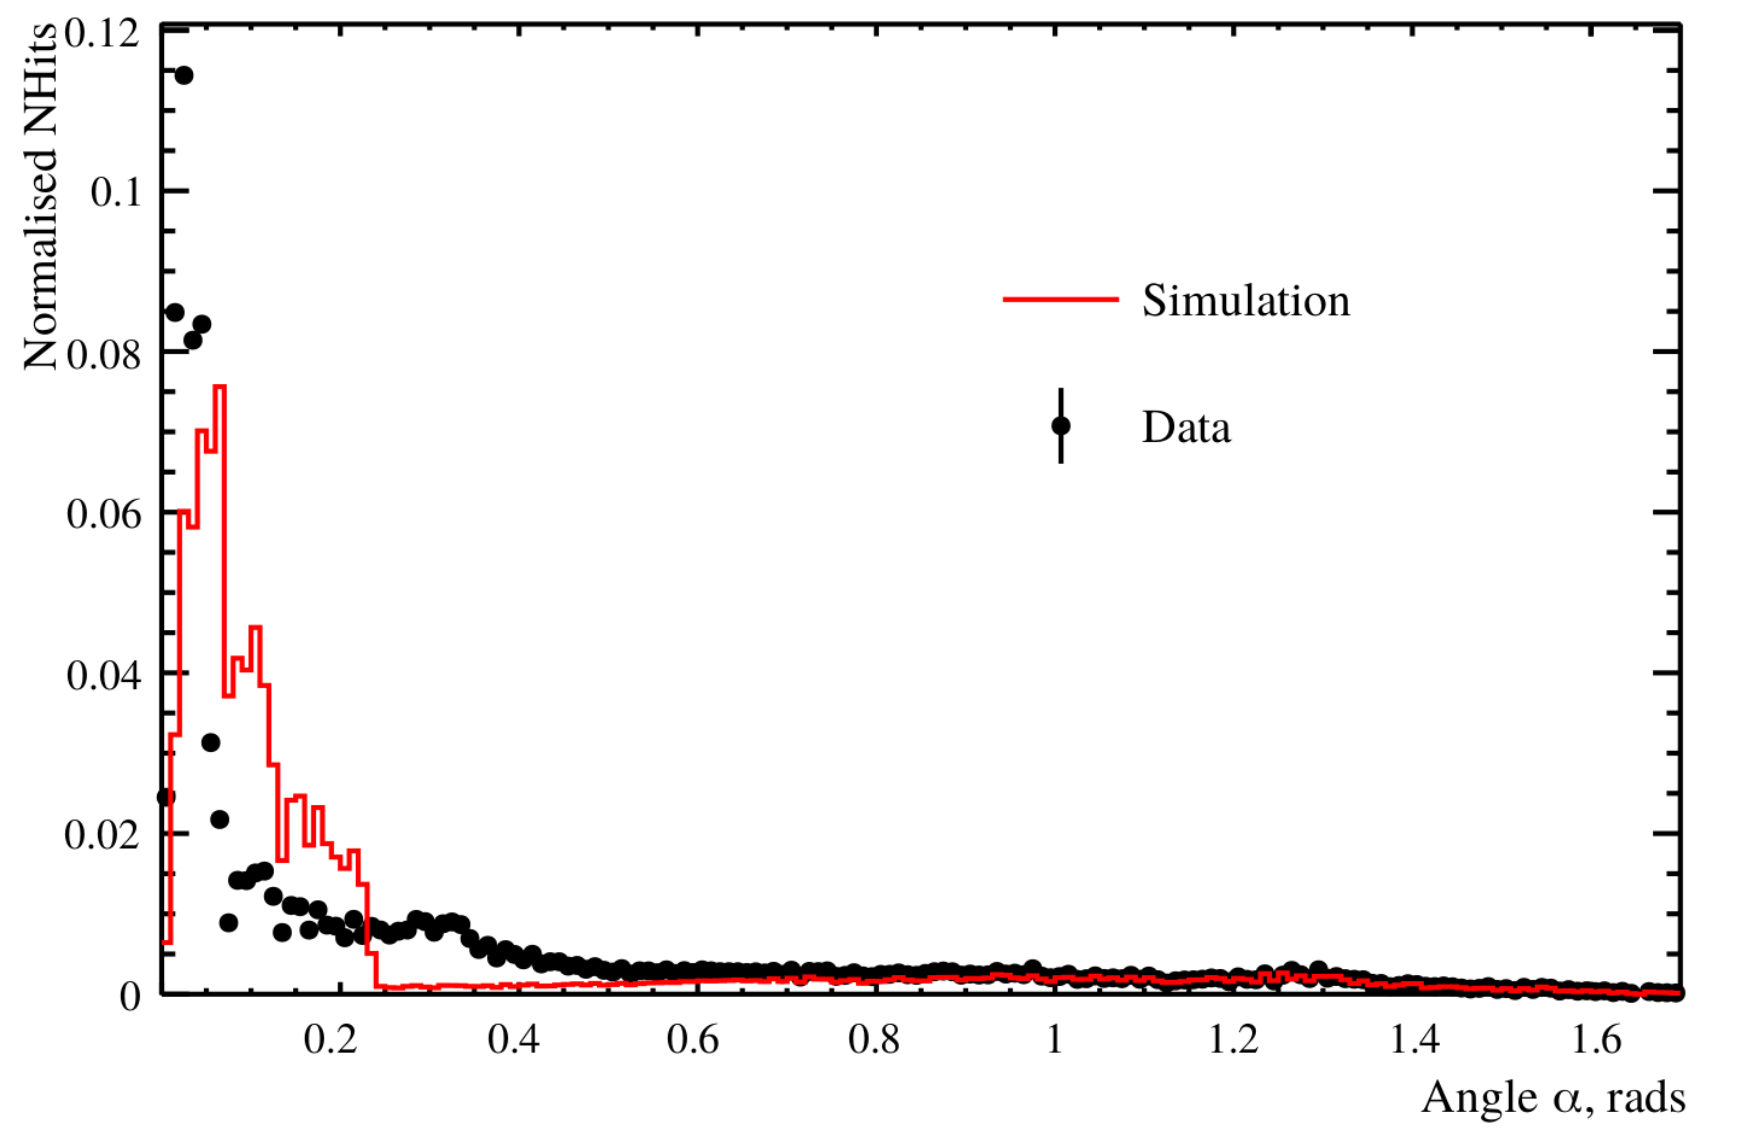
\includegraphics[width=0.7\textwidth]{4_SMELLIESimulation/images/1D_gen_plot.png}
    \caption[Comparison of SMELLIE between data and MC using a 1D generator]{Comparison between a simulation of one of the fibres, made from the 1D beam profile generator (red), with the associated data subrun that was used to create that beam profile (in black). For both MC and data, what is plotted is the PDF of observed PMT hits, as a function of the $\alpha$ angle. Poissonian errors have been added to the data points, but are too small to see. Clearly, this 1D generator does not replicate the observed beam profile correctly. Figure taken from~\cite{turnerMeasurementScatteringCharacteristics2022}.}
    \label{fig:1d_gen_plot}
\end{figure}

This 1D beam profile approach was used initially for SMELLIE, and remains in use for the other ELLIE sub-systems within SNO+. However, when SMELLIE data was taken in the water-phase of the experiment, simulations using these beam profiles failed to match them well at all - see figure~\ref{fig:1d_gen_plot} for an example. Not only was the distribution in $\alpha$ not Gaussian, a distinct speckle-pattern can be observed within the beamspot that is not uniform in $\phi$. This fact led to colleague Esther Turner building a SMELLIE generator that could handle 2D beam profiles: dependent on both $\alpha$ and $\phi$. The distribution was stored as a map from each inward-pointing PMT in the detector to a relative intensity value. This was chosen because the beam profile shapes were calibrated from existing SMELLIE data --- more on this in section~\ref{sect:new_beam_profiles}.

This original 2D generator then sampled the beam profile via a rejection sampling approach, outlined as follows:
\begin{enumerate}
    \item Propose a test direction $(\alpha, \phi)$, by generating $\phi$ uniformly in the interval $[0, 2\pi]$, and $\alpha$ according to some pre-determined Gaussian distribution, known as the Gaussian envelope.
    \item Given this test direction, calculate where a line following this direction from the fibre of interest will hit the PSUP on the other side of the detector. Find the 3 closest PMTs to that point.
    \item From those PMTs, obtain their relative intensity values from the beam profile mapping, and perform an interpolation based on how close each PMT is to the PSUP intersection point. This gives an interpolated relative intensity value for this test direction.
    \item Because we are sampling using the angular coordinates $(\alpha, \phi)$, differential area elements over this space of directions do not have the same size. We can correct for this fact by multiplying our interpolated relative intensity by $\sin{\alpha}$, which corresponds to the Jacobian of the direction-space.
    \item Calculate the value for the Gaussian envelope along this test direction.
    \item Throw a random number uniformly between 0 and the Gaussian envelope value. If the random number is less than the interpolated intensity, then this test direction is accepted, and a photon is generated with that direction. Otherwise, we reject the direction and try the whole process again.
\end{enumerate}

This generator certainly works, but has a key problem: efficiency. The 1D generator was able to generate a SMELLIE event (that is, to fully specify the starting parameters of all the photons emitted from a fibre) at a speed of $\sim\SI{1}{\milli\second}$. However, the 2D generator specified here could take upwards of $\sim\SI{50}{\second}$ \textit{per event} to generate. Because a typical SMELLIE analysis requires simulating many millions of events, the CPU time taken to perform this quickly became unfeasible. Fixing this generator speed problem was a high priority for the SMELLIE analysis.

\subsection{The new generator}\label{sect:new_gen}
On careful inspection of the existing 2D generator, the main reason for the slowness of the algorithm is the use of a rejection approach. Even with use of the Gaussian envelope, which was included to help with speed, the vast majority of proposed directions are never selected. Figure~\ref{fig:num_attempts} shows a histogram of number of attempts per event it took for a valid direction to be chosen for a representative SMELLIE simulation. Moreover, the calculations needing to be done for every proposed direction are relatively complex, notably trying to find the 3 nearest PMTs to some point on the PSUP.

\begin{figure}
    \centering
    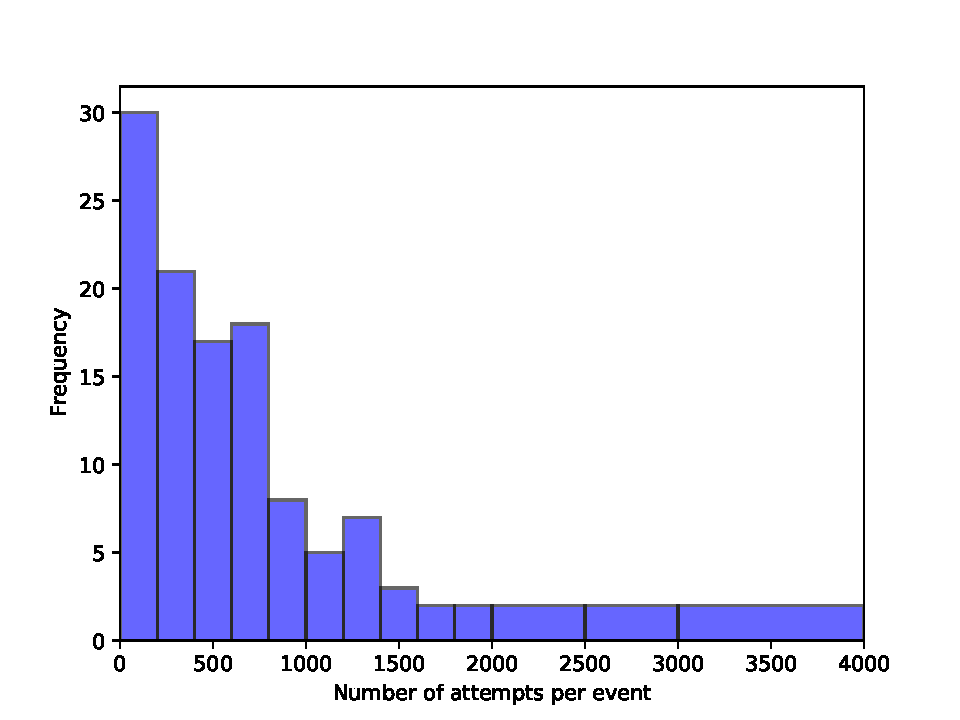
\includegraphics[width=0.7\textwidth]{4_SMELLIESimulation/images/2D_generator_num_attempts_nicer.pdf}
    \caption[Number of attempts taken for existing 2D SMELLIE generator to accept direction]{Typical distribution of the number of attempts it takes for the existing 2D generator before the test direction gets accepted, per event.}
    \label{fig:num_attempts}
\end{figure}

A new 2D generator was built with these thoughts in mind. Firstly, the rejection method would no longer be used, given its inefficiency. We would also endeavour to try and ``pre-calculate'' as much as possible before run-time. Starting with the existing PMT relative intensity maps, we plot these in the 2D direction-space $(1-\cos\alpha, \phi)$: see Figure~\ref{fig:esther_beam_profile}. In a toy-MC simulation, \num{500000} directions are then thrown uniformly in this 2D space per fibre. For each direction, the same method of obtaining an interpolated intensity value from the nearest PMTs to the corresponding point on the PSUP as from the original 2D generator was performed, the only difference being that these calculations were done well before any actual SMELLIE simulation. Figure~\ref{fig:old_profile_interpolated_sample_plot} shows the interpolated intensities obtained for one fibre.

\begin{figure}
    \centering
    \begin{subfigure}{0.98\textwidth}
        \centering
        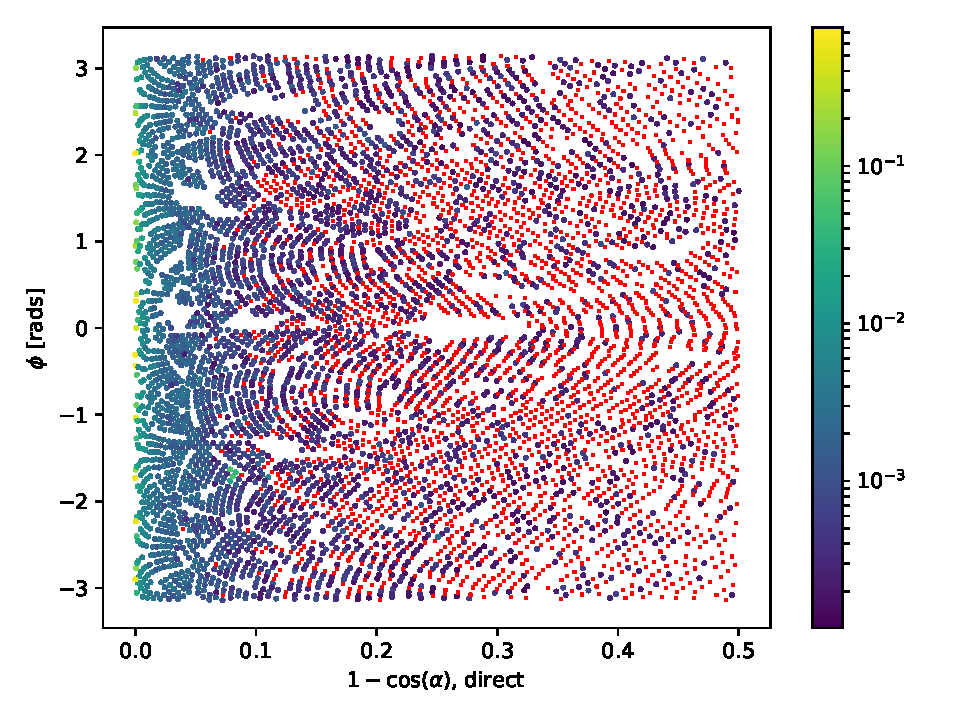
\includegraphics[width=0.74\textwidth]{4_SMELLIESimulation/images/flat_plot_r_FS055_beam_profile_original_6-18-13.pdf}
        \caption{PMT relative intensity map}
        \label{fig:esther_beam_profile}
    \end{subfigure}
    \begin{subfigure}{0.98\textwidth}
        \centering
        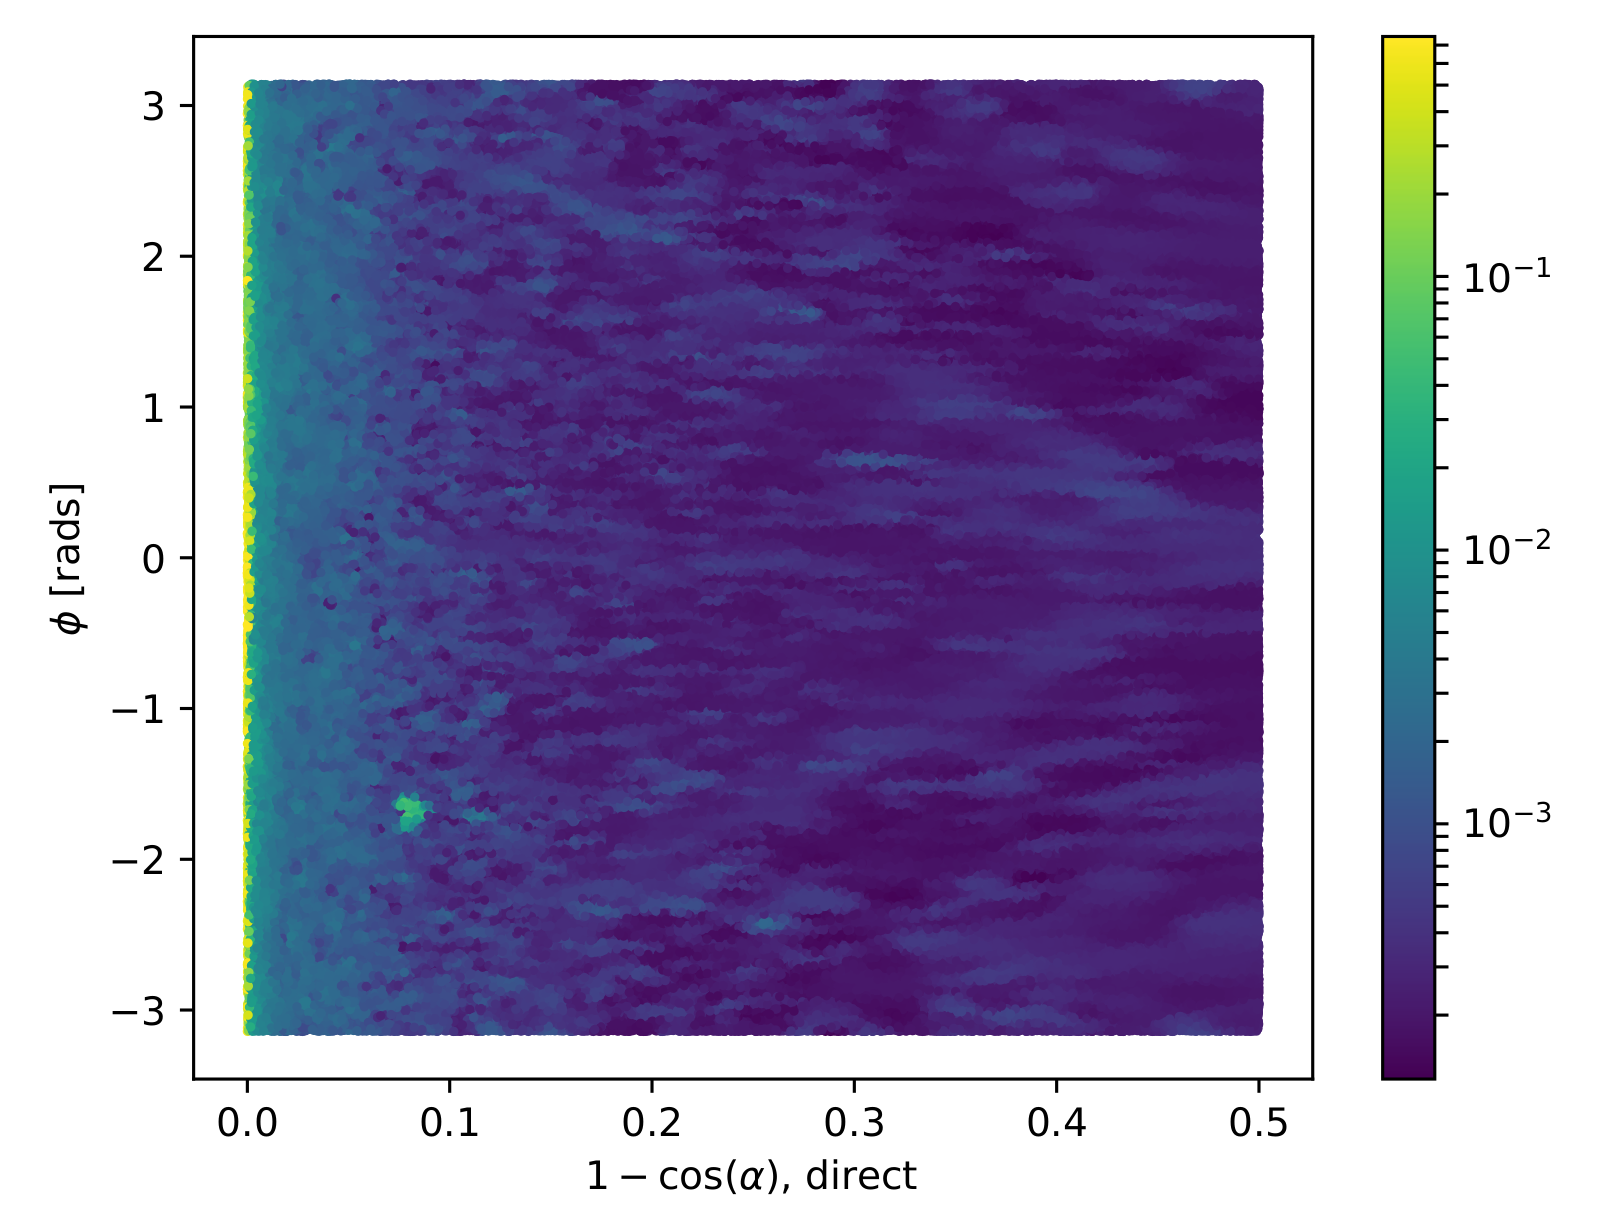
\includegraphics[width=0.74\textwidth]{4_SMELLIESimulation/images/polar_plot_FS055_MC_sampling_old_beam_profile.png}
        \caption{Interpolated intensity map}
        \label{fig:old_profile_interpolated_sample_plot}
    \end{subfigure}
    \caption[Intensity map of existing beam profile, and interpolated sampling map]{The first step in the new method for preparing the new generator. In (a), the relative intensities used for the existing beam profile of fibre labelled FS055 are shown for each PMT, the position on the plot indicating the location of that PMT in the fibre coordinates. The colour indicates the relative intensity; PMTs marked red have an intensity of zero. Figure (b) shows the result of throwing \num{500000} directions uniformly over this 2D space, the intensity of each point given by interpolating the intensities of nearby PMTs.}
    \label{fig:esther_beam_profile_and_interp}
\end{figure}

Following this, the sampled intensities were then binned into a 2D histogram, where the bin value corresponds to the sum of all intensities for all directions found within this bin. Choosing a sensible binning procedure is important: too few bins, and necessary information about the shape of the beam is lost, whilst too many bins can oversample the data and capture statistical artefacts in the sampling process instead of just the beam profile. As a balance, 15 bins were chosen along the $\phi$ direction, and 60 in $r=1-\cos\alpha$. This was chosen to ensure that a reasonable number of PMTs were located within each bin, lessening the impact of any statistical fluctuations. Although the bins in $\phi$ were chosen to have uniform width, this was decided to be not the case for the other axis, as there is far more important information near $r = 0$ (the beamspot). Instead, the width of the bins in $r$ were calculated so that roughly the same total probability was contained in each $r$-strip. By consequence, bins near the beamspot typically are of significantly smaller size than ones much further out. This allows us to both capture any rapid changes in intensity near the beamspot, where this matters greatly, and smooth out the very-low intensities seen at larger polar angles. One of these histograms can be seen in Figure~\ref{fig:hist_cdf_old_profile}: the large change in bin widths as a function of $r$ is clear. One can also see that near the beamspot notable dependence on the intensity as a function of $\phi$. The mysterious ``spot'' at $r = 0.08$, well out of the beamspot, is an indication that the underlying beam profile data being used requires improvement: more on this in section~\ref{sect:new_beam_profiles}.

\begin{figure}
    \centering
    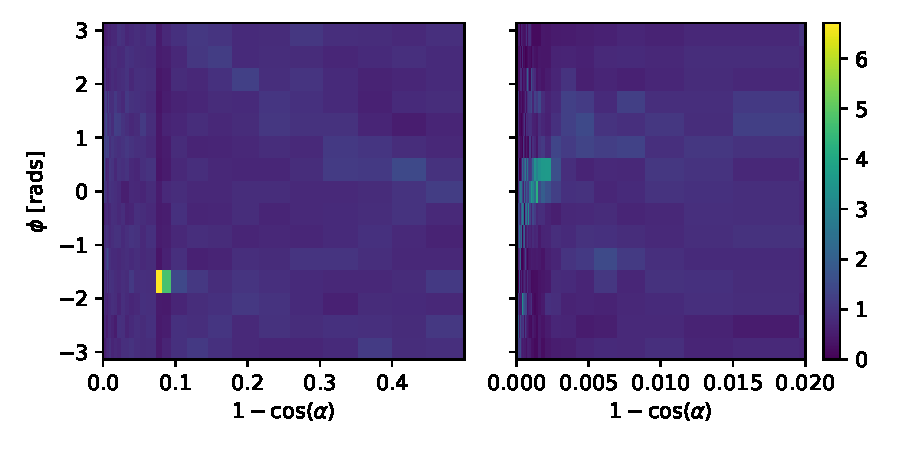
\includegraphics[width=\linewidth]{4_SMELLIESimulation/images/FS055_60_alpha_15_phi_hist.pdf}
    \caption[Histogram of interpolated intensities within the 2D direction-space]{Histogram of interpolated intensities within the 2D direction-space. The left view shows the full histogram; the right is a zoomed-in version near the beamspot. Unlike the binning in $\phi$, the bin widths in $r$ are not at all uniform. Instead, they have been determined such that the area summed over a given ``strip" of bins of constant $r$ will be the same.}
    \label{fig:hist_cdf_old_profile}
\end{figure}

The Cumulative Density Function (CDF) of this intensity histogram as a function of bin was then produced, where the bins were ordered through a raster-scan: scanning first over $\phi$, and then $r$. The CDF was then normalised to 1 so that it was well-defined. It is this CDF object that is then loaded in and sampled from during event generation. To do this, an ``inverse-CDF'' approach was used, which has the major benefit over rejection sampling of always producing a valid direction for every sample made. The algorithm works as follows:

\begin{enumerate}
    \item Throw a random number uniformly in $[0,1]$.
    \item Perform a binary search to find the bin that has the largest CDF value below this random number.
    \item Look at the bin edges in $\phi$ of this selected bin: use linear interpolation of the random number to obtain a $\phi$ value located between these two $\phi$-values.
    \item Look at the selected bin's $r$-bin edges, and select a value of $r$ by throwing a second random number uniformly between the two edges. Convert this $r$ into a polar angle $\alpha$.
    \item The photon's direction is defined by the $(\alpha, \phi)$ chosen by this process. 
\end{enumerate}

Because of the relative simplicity of this algorithm compared to the previous 2D generator, the speed improvement was very large: generation now took $\sim\SI{1}{\milli\second}$ per SMELLIE event, a speed improvement of nearly $\num{50000}$. Event generation became as fast as it was when the 1D generator was being used. Furthermore, because of the approach taken, this major speed improvement comes at no sacrifice in accuracy. Figure~\ref{fig:data_generator_comp_new_profiles} shows a comparison of the average number of photoelectrons (npe) per event per PMT between water-phase SMELLIE data and simulations with both the old and new 2D generator. One can see clearly that both generators are as accurate as one another. Note that this plot uses the updated beam profiles as explained in the next section.

\begin{figure}
    \centering
    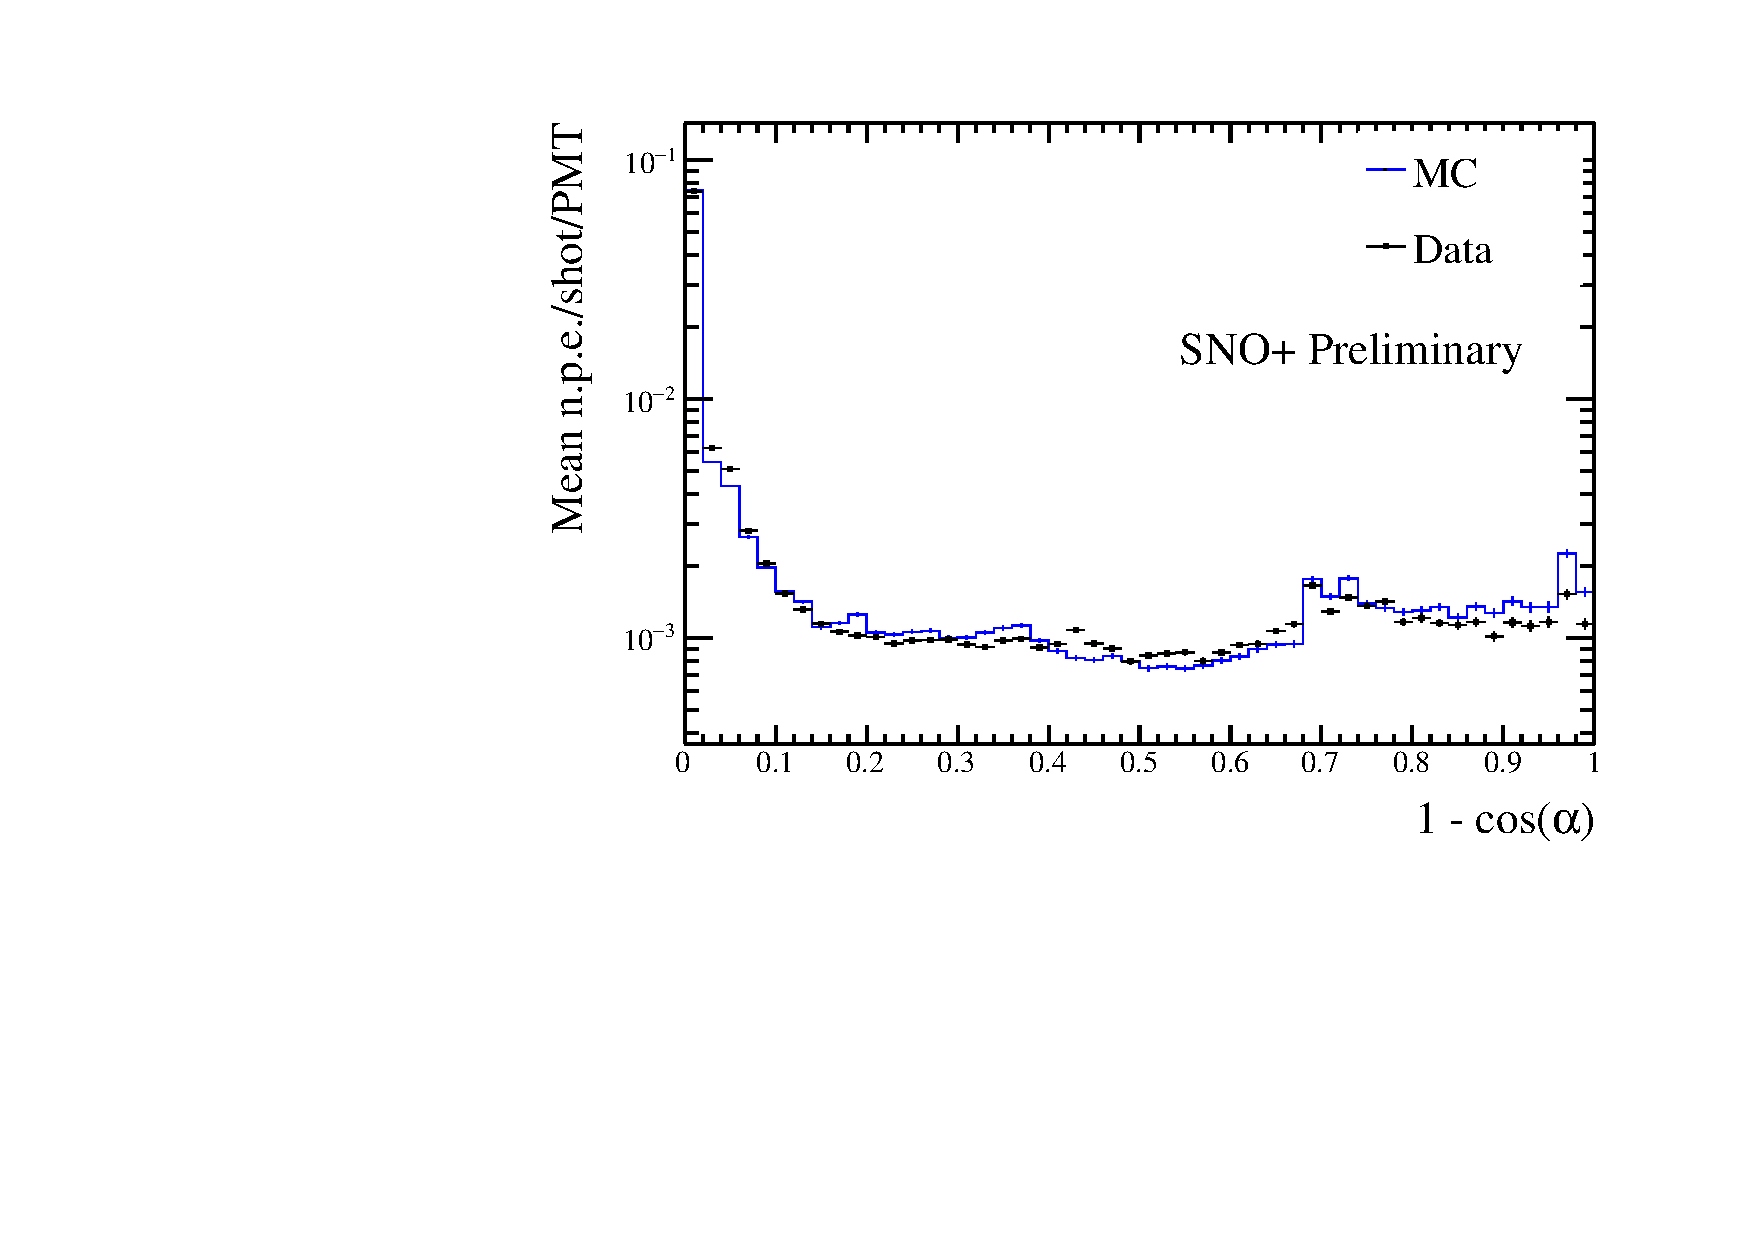
\includegraphics[width=\linewidth]{4_SMELLIESimulation/images/data_mc_comparison_npe_vs_r_114018_109_use_f.pdf}
    \caption[Comparison of water-phase data to MC generated using both the old and new 2D beam profile generator approaches, with the updated beam profiles]{Comparison of water-phase data to MC generated using both the old and new 2D beam profile generator approaches, with the updated beam profiles. Both versions of the generator are consistent with one another, but the new generator is many times faster.}
    \label{fig:data_generator_comp_new_profiles}
\end{figure}

\section{Improving the beam profiles}\label{sect:new_beam_profiles}
Even with the new 2D profile generator, a problem remains: the simulation fails to reasonably recreate data, and much of this appears to be because of the poor beam profile data being used. The curious ``spot'' for one of the fibres was already noted in the previous section that doesn't seem to be physical, and more broadly at large angles for all the fibres there are large swathes of PMTs with an intensity of zero, providing little useful information about the beam shape. It was shown in~\cite{turnerMeasurementScatteringCharacteristics2022} that with the old 2D generator, the systematic uncertainty on the beam profiles was the dominant source of error in the main SMELLIE analysis. To help improve this situation, it was decided to update the existing beam profiles.

These old beam profiles were originally determined by looking at SMELLIE data taken during the water-phase. Specifically, a ``medium''-intensity subrun with one of the lasers firing at a wavelength of \SI{495}{\nano\metre}, was chosen for each fibre. ``Medium''-intensity corresponds to firing the relevant laser at a set intensity determined during an earlier commissioning process, for which the maximum occupancy of PMT hits at that intensity, i.e. the proportion of hits per event, corresponded to roughly 80\%. This value was chosen as it allowed for high statistics in a relatively short run-time, but not so intense that the occupancy of any given PMT in the beamspot was 100\%. Because Rayleigh scattering is strongly-dependent on wavelength, the long wavelength of light was chosen so that impacts from this scattering were small in the data.

SNO+ PMTs are unable to distinguish the exact number of photoelectrons being generated. One is typically only able to know if a PMT has been triggered at all, by any number of photoelectrons. As a result, the occupancy of a PMT over a number of SMELLIE events, $o$, is a biased estimator of the mean number of photoelectrons generated, $\mu$. Assuming the number of photoelectrons generated in a given event follows Poisson statistics, the probability of generating $k$ photoelectrons is:

\begin{equation}
    P\left(k | \mu\right) = \frac{\mu^{k}e^{-\mu}}{k!}.
\end{equation}

The probability of observing a ``hit'' in a given PMT corresponds to generating at least one photoelectron:

\begin{equation}\label{eq:p_hit}
    P\left(\text{hit}| \mu\right) = P\left(k\geq 1 | \mu\right) = 1 - P\left(k = 0 | \mu\right) = 1 - e^{-\mu},
\end{equation}
which implies after rearrangement that one can determine the mean number of photoelectrons per event from the occupancy by:
\begin{equation}\label{eq:multihit_correction}
    \mu = \ln\left(1 - o\right).
\end{equation}
This is the reason why we want to avoid PMTs with occupancies of 100\%: they preclude one's ability to convert into a value for $\mu$ by looking at occupancy alone. We call this conversion from occupancy into npe the ``multi-hit correction''. The impact of this correction is typically small for most PMTs, but can become very significant in a fibre's beamspot.

Once the npe mapping from data was obtained, a correction was then made for the detector's optics: even ignoring a fibre's beam profile, we still expect certain PMTs to be illuminated more than others because of e.g. reflections off the AV, or the solid angle subtended by the PMT bucket opening. For each fibre, a simulation was made where the beam profile was set as isotropic, and the corresponding npe mapping obtained: this map held information about the detector optics only. The beam profile mapping was then derived by simply dividing each fibre's npe mapping from data to its associated isotropic MC npe map. It is these maps that were first used in section~\ref{sect:new_gen}.

\subsection{Combining beam profile datasets}
% \begin{center}
    \begin{table}
        \begin{tabular}{c p{6cm} p{6cm}}
            \hline
            Run Number & Run Type & Comments \\ \hline \hline
            \num{114018} & All PQ lasers; SuperK laser in \SIrange{400}{500}{\nano\metre} range & Only PQ495 laser and SuperK at \SI{495}{\nano\metre} is used \\
            \num{114023} & SuperK laser in \SIrange{500}{600}{\nano\metre} range & Part 1 of this wavelength range; crash occurred on last subrun, so that subrun is ignored \\
            \num{114034} & SuperK laser in \SIrange{500}{600}{\nano\metre} range & Part 2 of this wavelength range \\
            \hline
        \end{tabular}
        \caption{Water-phase runs used for new beam profiling.}
        \label{tab:runs_used}
    \end{table}
% \end{center}
Fortunately, much more SMELLIE data was taken during the water-phase than was used for the original beam-profiling analysis. This additional data can be combined with that which was already used to far better constrain the beam profiles. In particular, given the existing assumption that scattering effects are minimal above wavelengths of $\sim\SI{490}{\nano\metre}$, all data taken with wavelengths above this can also be used. The specific runs (and associated comments about their specifics) are described in Table~\ref{tab:runs_used}. Because high-intensity runs require a different analysis approach (PMTs with high occupancies must use charge, not occupancy, to  estimate npe), for this analysis we only considered subruns that used low or medium intensity set-points.

For each subrun $j$ of data per fibre, we look only at PMT hits for each PMT $i$ that has been identified as ``good'' for that subrun\footnote{Strictly speaking, a PMT's ``goodness'' is only determined on a run-by-run, not a subrun-by-subrun level, but this has no impact on the analysis.}, $i \in G_{j}$. $G_{j}$ here represents the set of good PMTs in subrun $j$. In particular, a ``good'' PMT must have valid electronic and timing calibrations, be at high voltage and masked into the detector's trigger system for that subrun. In addition, an angular cut of $\alpha < \SI{60}{\degree}$ was made to remove PMTs that are well outside any reasonable beam direction. To isolates the hits arriving directly from the fibre without reflecting, scattering, or being noise, a time cut was also made. Because what matters is the time relative to emission from the fibre, and the expected time-of-flight from fibre to different PMTs varies, a quantity known as the time residual was used. Starting with the calibrated hit time of a given PMT relative to the event's trigger time, $t_{hit}$, the expected time-of-flight $t_{TOF}$ from the fibre to the PMT was subtracted, estimated with the collaboration's ``Light Path Calculator''. Then, the emission time was also subtracted, $t_{emm}$, estimated by looking at the second-earliest value of $t_{hit}-t_{TOF}$ within the fibre's central beamspot, defined as the PMTs for which $\alpha<\ang{3}$. It was found that a ``loose'' time residual cut of $t_{res} \in [-10, +12] \si[]{\nano\second}$ was sufficient to remove the vast majority of non-direct light with little signal sacrifice. In the situation where a subrun with intensity was very small, it would not regularly have at least two hits in the beamspot, and so the time residuals calculated would not be valid for many events. To avoid this situation, a cut was made on any subruns with mean intensities below 9 within their beamspot. This value was chosen as it would mean a $2\sigma$ fluctuation downwards of $2\cdot\sqrt{9}=2\cdot3=\SI{6}{\npe}$ would still have more than the 2 hits necessary for timing reconstruction. One fibre, FS207, has no data subruns that satisfy this condition, and as such will have to be dealt with separately. For the time being, this fibre was ignored.

Extracting the underlying beam profiles from these data required some careful thought, especially because different subruns could have different intensities. Considering a PMT $i$ in subrun $j$, the mean number of photoelectrons generated per event in that PMT for that subrun, $\mu_{ij}$ can be decomposed as follows:

\begin{equation}\label{eq:mu_def}
    \mu_{ij} = I_{j}k_{i} = I_{j}b_{i}f_{i}.
\end{equation}
$I_{j}$ is the intensity of the subrun, i.e. the mean number of photons generated from the fibre in that subrun per event. $k_{i}$ is the probability that a given photon generated at the fibre source ends up generating a photoelectron in PMT $i$. This itself can be further split into two components: $b_{i}$, the probability that a given photon at the fibre source points in the direction of PMT $i$; and $f_{i}$, the probability that a given correctly-pointed photon actually makes it to the PMT and successfully generates a photoelectron. It is $b_{i}$ that is the actual beam profile we would like to measure.

Letting $p_{ij}$ be the probability of observing a hit for a given event on a given PMT, the probability of observing $m_{ij}$ hits out of $N_{j}$ events in the subrun will be binomially-distributed:
\begin{equation}
    P(m_{ij}| \mu_{ij}) = L(\mu_{ij} | m_{ij}) = \binom{N_{j}}{m_{ij}}p_{ij}^{m_{ij}}(1-p_{ij})^{N_{j}-m_{ij}} = \binom{N_{j}}{m_{ij}}\left(1-e^{-\mu_{ij}}\right)^{m_{ij}}e^{-\mu_{ij}(N_{j}-m_{ij})}.
\end{equation}
Here we have used equation~\ref{eq:p_hit}, and noted that this probability distribution in $m$ can be re-framed as a likelihood function for the parameter $\mu_{ij}$. Considering only a single subrun of data, the maximum likelihood estimate of the parameter $\mu_{ij}$ can be shown to be:
\begin{equation}
    \left<\mu_{ij}\right> = -\ln\left(1-\frac{m_{ij}}{N_{j}}\right) = \ln\left(1-o_{ij}\right) \qquad(m_{ij} \neq N_{j}),
\end{equation}
where $o_{ij}$ is just the occupancy of PMT $i$ in subrun $j$. This is just the multi-hit correction formula seen in equation~\ref{eq:multihit_correction}, which makes sense.

When looking at multiple subruns for the same fibre, the total likelihood function for a given PMT when considering all the data for a given fibre will be the product of the likelihoods from each dataset,
\begin{equation}
    L\left(\left\{I_{j}\right\}, k_{i} | \left\{m_{ij}\right\}\right) = \prod_{j} L(I_{j}, k_{i} | m_{ij}) = \prod_{j}\binom{N_{j}}{m_{ij}}\left(1-e^{-I_{j}k_{i}}\right)^{m_{ij}}e^{-I_{j}k_{i}(N_{j}-m_{ij})}.
\end{equation}
This leads to a log-likelihood distribution of
\begin{equation}
    \mathcal{L}\left(\left\{I_{j}\right\}, k_{i} | \left\{m_{ij}\right\}\right) = \sum_{j}\left[\ln\left(^{N_{j}}C_{m_{ij}}\right) + m_{ij}\ln\left(1 - e^{-I_{j}k_{i}}\right) - I_{j}k_{i}\left(N_{j} - m_{ij}\right)\right].
\end{equation}
Formally, one could combine the likelihoods of all the PMTs together, and by looking at the maximum likelihood estimates for each of the parameters measure the parameter values this way. However, the set of equations one obtains through this approach quickly become analytically intractable, because the PMTs are coupled by the intensity values $I_{j}$. Even a direct numerical approach would be liable to fail: for a given fibre there can be dozens of subruns, and many thousands of PMTs of relevance, so the dimensionality of the system of equations would be far too large.

Because of this, a different approach was taken. It is expected that in a subrun the total npe, summed over all good PMTs, should be proportional to the intensity value $I_{j}$. One must be careful about this construction --- different subruns can have different sets of good PMTs, so two subruns with identical $I_{j}$ values could have a larger summed npe merely because more PMTs were good in that subrun. To counter-act this effect, only PMTs that were classified as good in \textit{all} subruns being analysed for that fibre would be used for the npe summation. In other words, we use data from PMT $i$ for summing only if:
\begin{equation}
    i \in \mathcal{I} = \bigcap_{j}G_{j}.
\end{equation}
We can then define the summed npe for a given subrun as $S_{j} = \sum_{i\in\mathcal{I}}\text{npe}_{ij}$, and assert that $I_{j} = cS_{j}$. By finding a value proportional to $I_{j}$, there is now enough information to maximise the log-likelihood $\mathcal{L}\left(k_{i} | \left\{m_{ij}\right\}, \left\{I_{j}\right\}\right)$ with respect to $k_{i}$ for each PMT independently, and hence obtain estimates for these $k_{i}$ parameters.

Of course, what is actually wanted are the underlying $b_{i}$ values, not $k_{i}$. This is where isotropic simulations come in. For each run of data used, a matching isotropic MC was produced. As an example, a simulation for run \num{114023} contained \num{200000} events for each fibre using an isotropic beam profile, over the full wavelength range considered in this run, \SIrange{500}{600}{\nano\metre}, using the same run conditions as in data (which PMTs were at high voltage, etc.).

For each isotropic MC run, both $I_{j}^{MC}$ and $k_{i}^{MC}$ were calculated via the method described above. Because the simulations were isotropic, the underlying value for $b_{i}$ was constant across all the PMTs, and so $ak_{i}^{MC} = f_{i}$. By doing some rearranging of equation~\ref{eq:mu_def}, we find that:
\begin{equation}
    \mu_{ij} = I_{j}b_{i}f_{i} = cS_{j}b_{i}ak_{i}^{MC} = (acb_{i})S_{j}k_{i}^{MC}.
\end{equation}
As a result of this, given the set $\left\{S_{j}\right\}$ and $k_{i}^{MC}$, one can maximise the log-likelihood $\mathcal{L}$ with respect to $b'_{i} = acb_{i}$ numerically, to obtain the maximum likelihood estimate of $b'_{i}$. Because $a$ and $c$ were global constants of proportionality, they would become irrelevant as soon as the beam profile was normalised in the CDF-creation process outlined in~\ref{sect:new_gen}.

Figure~\ref{fig:likelihood_scan} shows the shape of this log-likelihood distribution for a particular PMT when considering fibre FS007's beam profile. One can see how individual subruns provide much more information when combined than if one looked at a single subrun alone.

\begin{figure}
    \centering
    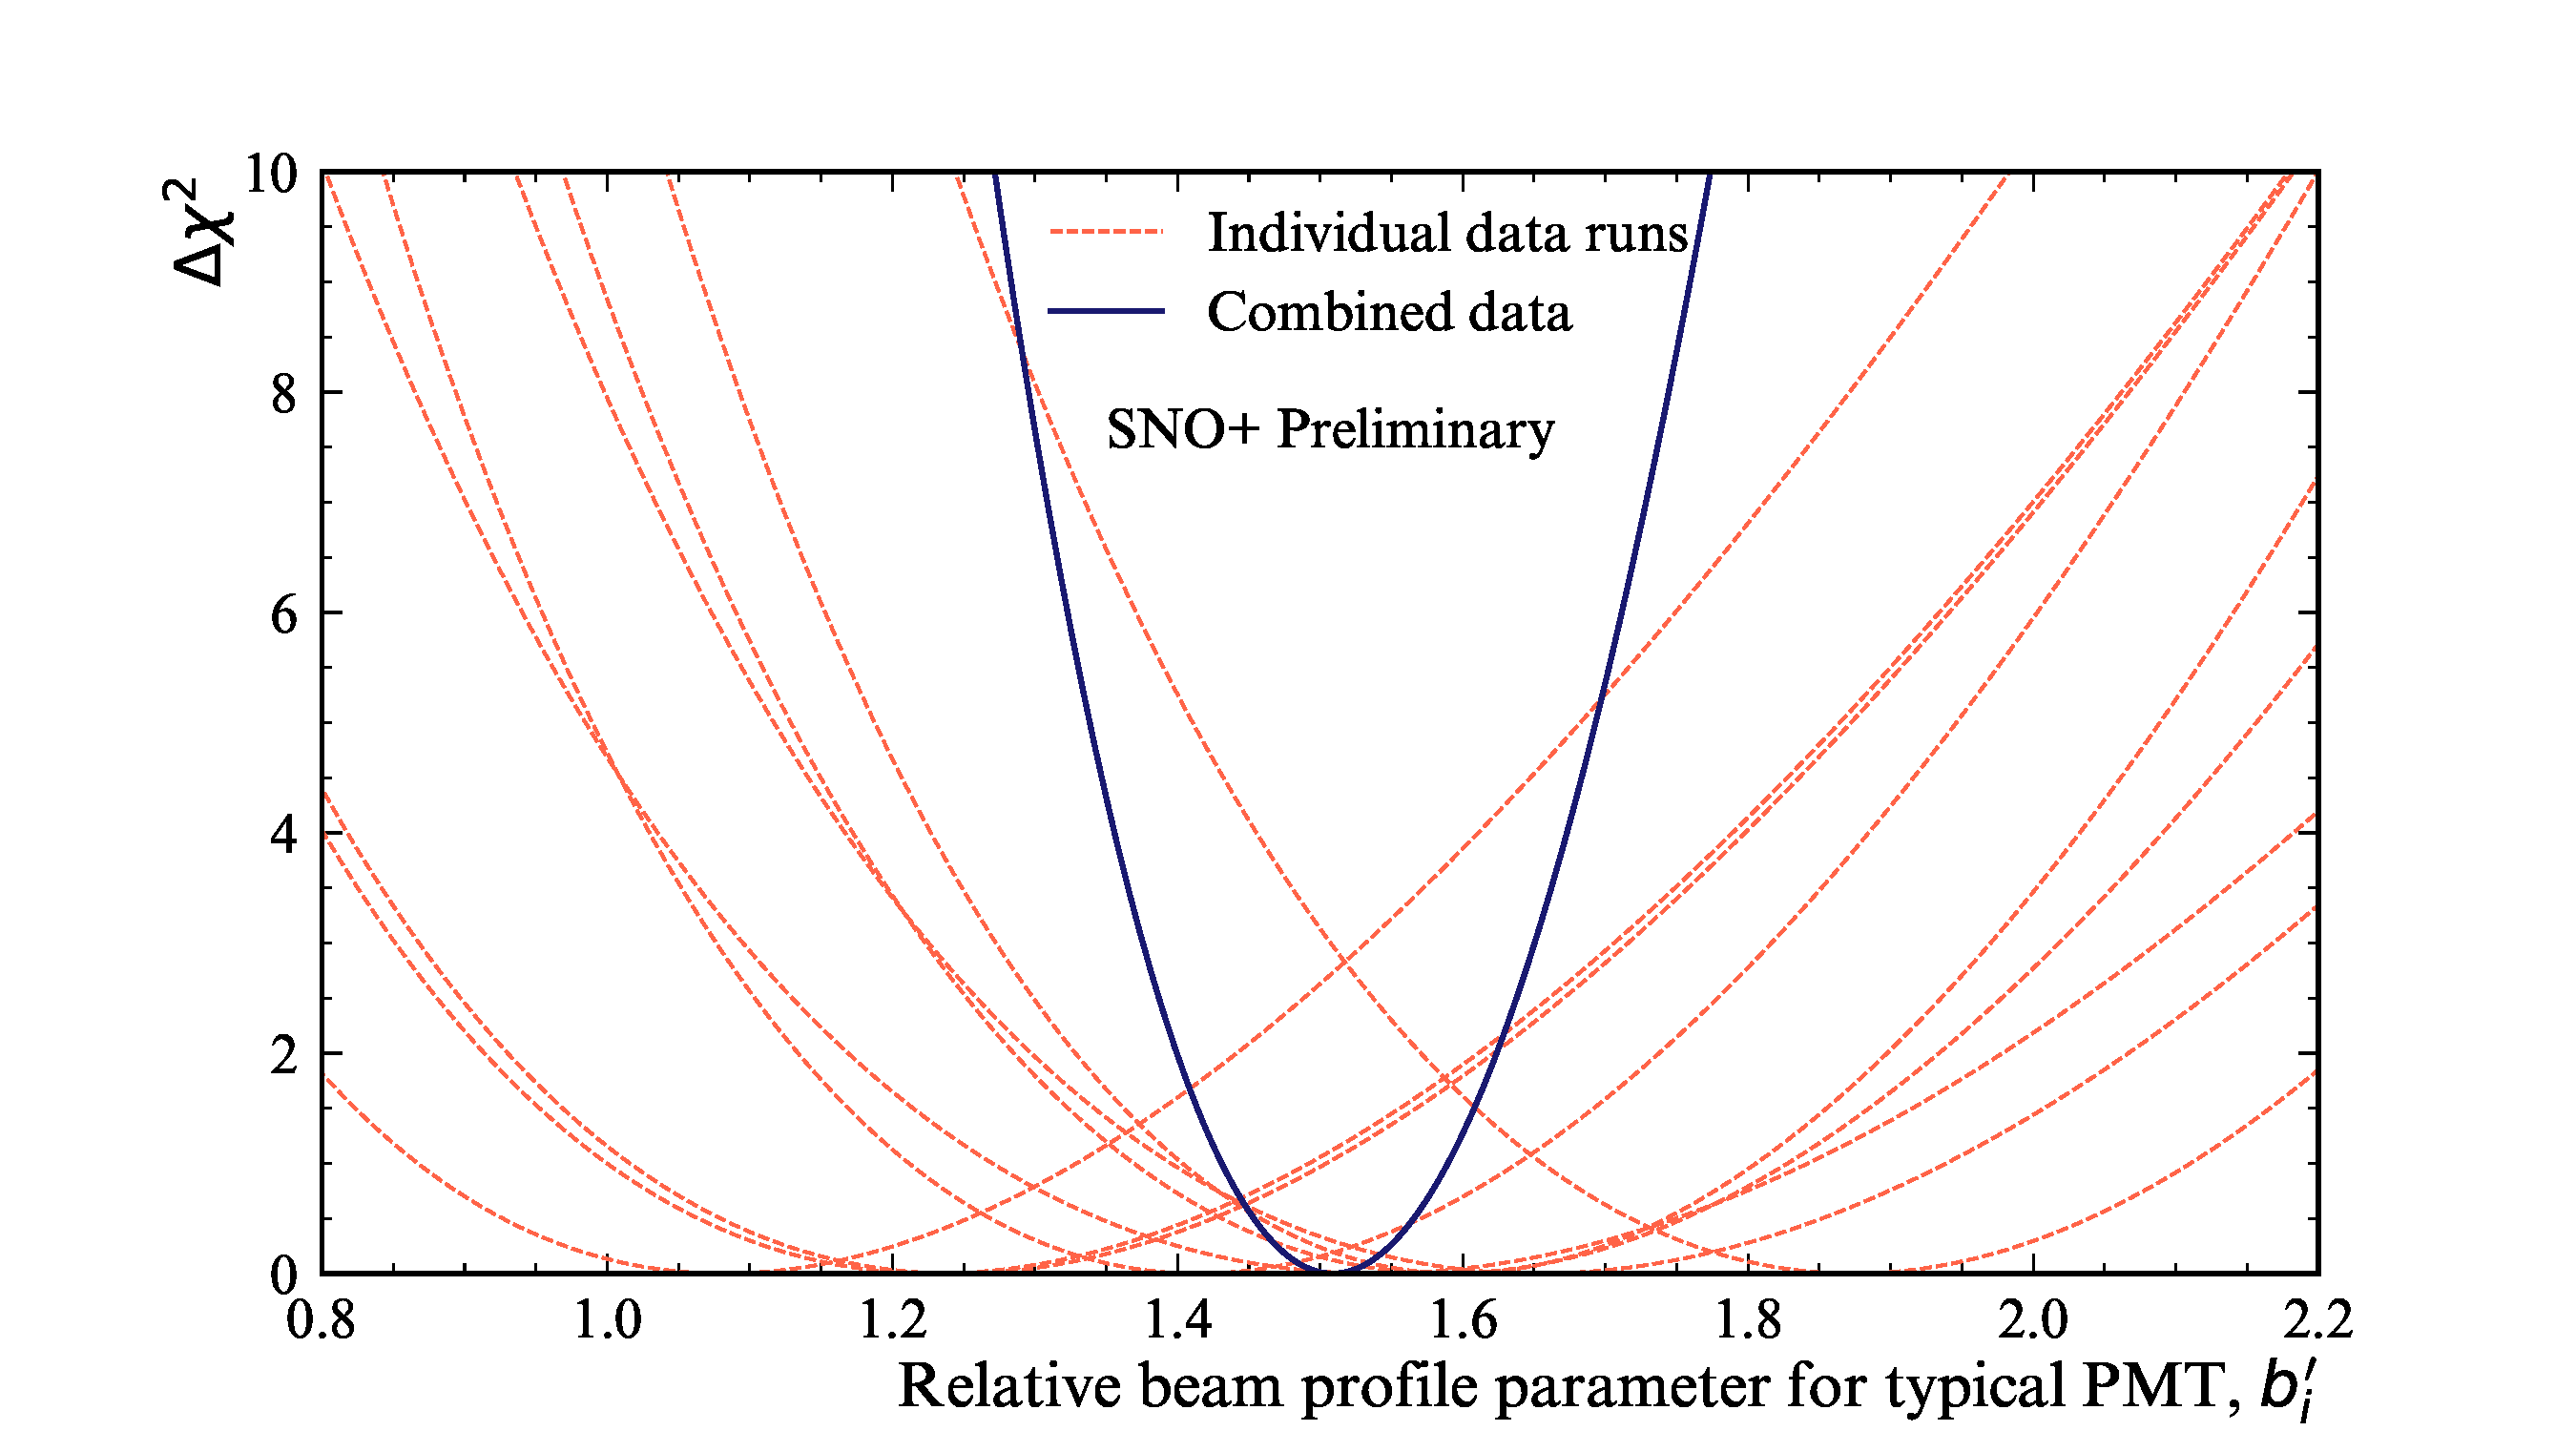
\includegraphics[width=0.8\linewidth]{4_SMELLIESimulation/images/example_likelihood_distribution_pmt_inc_all_subruns_proper_formatting.pdf}
    \caption[Plot of $\Delta\chi^2$ for both single subruns of a typical PMT, and when all relevant subruns are combined]{Plot of $\Delta\chi^2\simeq X_{i}$, twice the negative log-likelihood ratio, for both single subruns of a typical PMT, and when all relevant subruns are combined.}
    \label{fig:likelihood_scan}
\end{figure}

Another benefit of using this log-likelihood approach is that the resulting distribution's shape can be used for uncertainty estimation. In almost all cases, Wilks Theorem~\cite{wilksLargeSampleDistributionLikelihood1938} allows us to produce $1 \sigma$ confidence intervals about the maximum likelihood estimate for $b'_{i}$, $\left<b'_{i}\right>$, because $$X(b'_{i}) = -2\left[\mathcal{L}\left(b'_{i}\right) - \mathcal{L}\left(\left<b'_{i}\right>\right)\right]$$ approximates a $\chi^2$-distribution. As a result, the error bounds on our parameter estimate are given by when $X = 1$. The fact that the shape of $X$ can be well-approximated by a quadratic in the region near $X = 0$ indicates the validity of Wilks' Theorem being used here.

Only a couple of exceptions to this approach of parameter estimation are possible. In the case where $m_{ij} = N_{j}$, i.e. a PMT has 100\% occupancy, no maximum likelihood estimate exists: we need not worry about this, as subruns where this occurs have not been used. On the other end, however, there are some PMTs for certain fibres where after all subruns of data have been included, there remains no hits. In this scenario, one can show that the log-likelihood becomes linear in the beam profile parameter:
\begin{equation}
    \mathcal{L}\left(b'_{i}|\left\{m_{ij}=0\right\}\right) = b'_{i}k_{i}^{MC}\cdot\sum_{j}\left[I_{j}N_{j}\right].
\end{equation}
This scenario is very much reminiscent of rare-decay searches, and a similar approach can be used. A $1 \sigma$ upper limit on the possible value for $b'_{i}$ can be analytically-calculated to be:
\begin{equation}
    b'_{i,ulim} = -\frac{k_{i}^{MC}\sum_{j}\left[I_{j}N_{j}\right]}{\ln\left[1 - \operatorname{erf}\left(1/\sqrt{2}\right)\right]},
\end{equation}
where $\operatorname{erf}(x)$ is the error function.
{
    \color{blue}
    [18 pages for above two sections]
}

\subsection{Results \& Discussion}\label{sect:results}
{
    \color{blue}
    WARNING: contents of this subsection will be gutted, focusing merely on impact of combining data sets. Details about discrepancies will be covered in the next section.
    [Will just be ~1 page]
}
Figure~\ref{fig:updated_beam_profile} shows the impact of using additional subruns of data on a typical beam profile. One can clearly see the great reduction in the number of PMTs with no hits in data. That many more data sets were included allowed for the major increase in dynamic range available for measuring these $b'_{i}$ values. One can also note that by including additional data the curious spot that was seen in the old beam profile our at $r\approx0.08$ has gone, further indicating that it was an artefact of that single data set.
\begin{figure}
    \centering
    \includegraphics[width=0.8\textwidth]{4_SMELLIESimulation/images/flat_plot_r_comparison_FS055_old_vs_new_empty_circles.pdf}
    \caption[Comparison between old and updated beam profiles for fibre FS055, after combining multiple data sets]{Comparison between old and updated beam profiles for fibre FS055, after combining multiple data sets. Once again, the relative intensities ($b'_{i}$) for each PMT are given by the colour of each point, the position of each plotted in the 2D $(r,\phi)$-space. The relative intensities have been both scaled here so that the largest value equals 1. Hollowed-out points are PMTs that, even after all relevant subruns have been combined, have no PMT hits.}
    \label{fig:updated_beam_profile}
\end{figure}

Further details can be gathered from the interpolated intensity maps, one of which can be seen in figure~\ref{fig:updated_beam_profile_sampling}. There are two curious stand-out features that can be seen here: firstly, there are multiple distinct parabolic arcs. These correspond to the shadows of the ropes that hold up/down the AV. More precisely, they are the mismodelling of those shadows --- if the shadows were in the right place in the isotropic MC, then they would correctly cancel out any decreased intensity seen in the data of shadowed PMTs. These shadows could be mismodelled either because the positions of the ropes in the MC are in the wrong place, or the fibre's emission position is wrong. Note that any mismodelling of the fibre's nominal emission direction has no impact on this shadowing problem, as changing that direction merely causes a change of basis in the $(r,\phi)$-space. The latter possibility of incorrect fibre positions are more likely, and in fact these arcs in the beam profiles could be used as an effective way to correct for this problem.

\begin{figure}
    \centering
    \includegraphics[width=0.8\textwidth]{4_SMELLIESimulation/images/flat_plot_r_FS055_500k_interpolated_beam_profile_full_formatting.png}
    \caption[Interpolated intensity map for the new updated beam profile of fibre FS055]{Interpolated intensity map for the new updated beam profile of fibre FS055. The misalignment of rope shadows and AV effects, can both be seen.}
    \label{fig:updated_beam_profile_sampling}
\end{figure}
The second distinctive feature of this intensity map is the large band of lower intensity varying between $r\approx0.2-0.5$, followed by larger intensity out at large $r$ values. This feature comes from light reflecting off the AV surface, or internally-reflecting. The reason for this band's functional dependence on $\phi$ is that this particular fibre, FS055, has a nominal fibre direction $\sim\ang{10}$ from pointing radially-towards the detector's centre. This feature appears in the updated beam profiles of all fibres, but its shape depends on the particular fibre's direction --- for fibres pointing directly towards the detector's centre, there is little $\phi$-dependence observed. Like the ropes, this feature must come from some form of mismodelling of the optics of the AV. A de-facto shadowing of PMTs in line with tangents from the AV surface which intersect the fibre position is to be expected. One also expects PMTs at polar angles larger than this to have their observed intensities boosted from reflected light off the AV. However, the discontinuities seen in the beam profiles indicate that for whatever reason this effect has been over-emphasised in the simulation.

There is a further phenomenon that can be seen, by comparing beam profile values obtained from a single subrun to the updated combined beam profile. This can be done by calculating the residuals corresponding to the single subrun, relative to the combined data set. The residual is negative if the combined data sets have a $b'_{i}$ below the equivalent for a given single subrun; that is, the combined model underestimates this subrun for that PMT.

This information was plotted for two different subruns from the same fibre, seen in figure~\ref{fig:llr}. One subrun was the same one used by Esther Turner for the original 2D beam profiling, with a wavelength of \SI{495}{\nano\metre}; the latter was at the longer wavelength of \SI{595}{\nano\metre}. For both subruns, most PMTs are seen to have intensities well-modelled by the combined model. However, their appears to be a significant amount of mismodelling within the beamspot. There also appears to be some systematic shift between data and model at somewhat larger polar angles. Moreover, this mismodelling seems not to be merely random, but a function of wavelength: at shorter wavelengths the beamspot tends towards being overestimated and then underestimated at larger values of $\alpha$. At longer wavelengths, the beamspot becomes underestimated, with larger angles getting overestimated. This indicates that there appears to be a wavelength-dependence on the beam profiles, contradicting one of the main assumptions which we used to combine the water-phase data in the first place!
\begin{figure}
    \centering
    \includegraphics[width=\textwidth]{4_SMELLIESimulation/images/residual_wavelength_comparison_data_model_nice.pdf}
    \caption[Residuals from subruns at two different wavelengths, both compared to the combined beam profile model for fibre FS055]{Residuals from subruns at two different wavelengths, both compared to the combined beam profile model for fibre FS055. A negative sign, and hence bluer colours, indicate that the combined model underestimates the observed intensity for that particular subrun. Values with a magnitude beyond 5 are shown capped at this maximal value for the purposes of this plot. These PMTs are plotted in the polar fibre coordinates $(\alpha,\phi)$.}
    \label{fig:llr}
\end{figure}
All three of these features --- rope shadows, AV reflections, and wavelength dependence --- add systematic uncertainty to the beam profiles, beyond the statistical uncertainty as measured by the width of the likelihood distribution. Certainly if one wanted to further improve the uncertainties in the beam profiles, tackling these challenges would be key.

\section{Comparisons between Data and Simulation}\label{sec:smellie_systematics}
{
    \color{blue}
    \begin{itemize}
        \item This focuses on disagreements noticed between data and MC even after the new generator and beam profiles have been used.
        \item Important to mention that none of these are necessarily game-ending, they are just systematics that may or may not be substantial in a given analysis with SMELLIE..
    \end{itemize}
    
    \subsection{Forward Hemisphere Discrepancies}
    \begin{itemize}
        \item The continued disagreement between data and MC when it comes to measured npe in various parts of the ``forward" hemisphere. This includes:
        \begin{itemize}
            \item The central beamspot,
            \item The TIR region,
            \item Rope shadows,
            \item A noticeable wavelength-dependence.
        \end{itemize}
        \item This is pretty much most of the contents of Section~\ref{sect:results}.
    \end{itemize}
    [4 pages]
    
    \subsection{Emission Time Discrepancies}
    \begin{itemize}
        \item For certain lasers, a strong mismatch in the observed hit time residuals for prompt light.
        \item A mysterious +18 ns bump seen for the PQ495 laser.
        \item A trigger jitter in the SuperK laser.
    \end{itemize}
    [3 pages]
    \subsection{Backward Hemisphere Discrepancies}
    \begin{itemize}
        \item The observed distribution of hits vs time and angle in MC does not match data in a number of ways for PMTs near the fibre emission point.
        \item Includes the outer-water scattering length, rope reflections, and investigations into whether certain modifications to the optics could plausibly fix things (so far, no).
    \end{itemize}
   [6 pages]

   [32 PAGES TOTAL]
}
\chapter{Analysis of SMELLIE Data in the Scintillator Phase}\label{chap:smellie_analysis}
% \epigraph{\textit{}}{source}

This chapter contains two sets of analyses: measurements of the extinction lengths of the scintillator as a function of wavelength and time, as well as monitoring the Rayleigh scattering length over time. In both cases, care had to be taken to try and make the methodologies robust to systematics.

\section{Extinction Length Analysis}\label{sec:ext_length_analysis}
% \subsection{Motivation}
% \begin{itemize}
%     \item Explain motivating observations for this analysis: a substantial discrepancy between MC and data seen in the radial profiles of nhitsCleaned for \ce{^{210}Po} after the PPO top-up campaign. Performed by Serena.
%     \item Hypothesis of a shortening of the absorption/scattering length proposed, further strengthened by Ben Tam's ex-situ absorption measurements with scintillator taken from the detector, as well as knowledge about a likely ``cooking'' of PPO during the PPO-fill.
%     \item Describe the provisional optics model decided on based on these measurements, which includes an additional non-re-emitting component of the scintillator.
%     \item As a further cross-check, SMELLIE should be sensitive to changes in the overall extinction length of the scintillator, especially for short extinction lengths relative to the size of the detector.
%     \item More straightforward in measuring extinction length compared to scattering length --- no need to distinguish between scintillator re-emission and scattering.
%     \item Further uses: can be used to monitor the extinction length over time!
% \end{itemize}
% [4 pages]
The first analysis discussed in this chapter is the measurement of the extinction lengths of the liquid scintillator deployed in the SNO+ detector, as a function of both wavelength and time. As seen in Fig.~\ref{fig:smellie_timeline}, SMELLIE data was taken during the water phase, and in the scintillator phase when the PPO concentration of the LABPPO was at a variety of levels. Fig.~\ref{fig:smellie_expected_ext_length_phases} shows the expected changes in extinction length with detector phase, as a function of wavelength, according to the optical model described in Section~\ref{sec:optical_processes}.

\begin{figure}
    \centering
    % \includegraphics[width=0.8\textwidth]{6_SolarAnalysis/images/b8_eelectrue_vs_enutrue.pdf}
    \caption[]{}
    \label{fig:smellie_expected_ext_length_phases}
\end{figure}

\subsection{Analysis Approach}
\subsubsection{The 2-PMT Case}
To begin, consider light emission from a particular SMELLIE fibre of fixed wavelength $\lambda_{j}$, with a mean emission intensity of $I_{j}$ photons emitted per event in subrun $j$ during detector phase $p$. Modifying Eq.~\ref{eq:mu_def}, a general PMT $i$ will have a mean npe per event of $\mu_{ij,p}(\lambda_{j}) = I_{j,p}b_{i,p}(\lambda_{j})f_{i,p}(\lambda_{j})$. A detector phase-dependence has been added to all terms, because:
\begin{itemize}
    \item The emission intensities chosen, $I_{j,p}$, can vary between different data-taking campaigns. These changes are due to changes in hardware (as detailed in Chapter~\ref{chap:smellie_hardware}), as well as changes in the settings used to run SMELLIE.
    \item The beam profile of a given fibre at a given wavelength is not expected to change with detector phase. However, if the refractive index of the inner detector medium changes (e.g. from the water phase to scintillator phase), then the fraction of light emitted that is pointed in the correct direction to be detected by PMT $i$, $b_{i,p}(\lambda_{j})$, \textit{can} change. This effect is discussed in more detail in Section~\ref{sec:smellie_ext_corrections}.
    \item In a different phase of the detector, the optics of the inner detector can certainly change, and so the probability that a photon pointing in the correct direction for PMT $i$ actually makes it across the detector and generates a photoelectron, $f_{i,p}(\lambda_{j})$, can change.
\end{itemize}

For the purposes of this analysis, consider specifically PMTs in the beamspot of the fibre with unobstructed paths. Then, a given beamspot PMT will have a mean npe per event, $\mu_{ij,p}^{\mathrm{beam}}(\lambda_{j})$, of:
\begin{align}\label{eq:smellie_ext_length_theory}
    \mu_{ij,p}^{\mathrm{beam}}(\lambda_{j}) &= I_{j,p}b_{i,p}(\lambda_{j})
    \exp\left(
        -\frac{L_{ij,p}^{\mathrm{extern}}(\lambda_{j})}{l^{\mathrm{extern}}(\lambda_{j})}
    \right)
    \exp\left(
        -\frac{L_{ij,p}^{\mathrm{acr}}(\lambda_{j})}{l^{\mathrm{acr}}(\lambda_{j})}
    \right)
    \exp\left(
        -\frac{L_{ij,p}^{\mathrm{inner}}(\lambda_{j})}{l_{p}^{\mathrm{inner}}(\lambda_{j})}
    \right)\nonumber\\
    & \qquad\cdot T_{ij,p}(\lambda_{j})\epsilon_{ij,p}(\lambda_{j}).
\end{align}
Here, $L_{ij,p}^{\mathrm{extern,acr,inner}}(\lambda_{j})$ is the length of a path in a given detector medium through which light travels, for the external water, acrylic, and inner detector medium, respectively. $l_{p}^{\mathrm{extern,acr,inner}}(\lambda_{j})$ is the extinction length of each detector medium for a given wavelength --- it is assumed that only the inner detector medium has changing optics in different phases. Some fraction of light is lost when passing between two mediums with different refractive indices: this is captured by $T_{ij,p}(\lambda_{j})$, the product of the Fresnel transmission components for all optical boundaries along a photon's path. Finally, $\epsilon_{ij,p}(\lambda_{j})$ is the probability that a photon along a given path, incident on a given PMT, will generate a photoelectron that is detected. 

Measuring $l_{p}^{\mathrm{inner}}(\lambda_{j})$ is the aim of this analysis. In order to do so, all other parameters in Eq.~\ref{eq:smellie_ext_length_theory} must either be measured, or removed in some careful way. As discussed in Section~\ref{sec:optical_processes}, the extinction lengths of both the UPW and the acrylic were measured as a function of wavelength in the water phase with the Laserball. It is assumed that the optics of the UPW inside and outside the AV were the same, and have not changed since. That section also discusses the measured refractive indices as a function of wavelength for the UPW, acrylic, and LABPPO. For a given detector phase, subrun, and PMT, the Collaboration's \texttt{Light Path Calculator} is able to determine the values of $L_{ij,p}^{\mathrm{extern,acr,inner}}(\lambda_{j})$ as well as the combined Fresnel transmission coefficient $T_{ij,p}(\lambda_{j})$.

As will be discussed in Section~\ref{sec:smellie_intensity}, measuring the absolute value of $I_{j,p}$ is challenging. Fortunately, there are ways of making relative intensity calibrations, which is sufficient for this analysis. Consider PMTs near the fibre emission point. The first light observed by these PMTs will be from photons which have `back-scattered' off of the UPW outside the AV. This is followed by light reflected off of the AV surface. Fig.~\ref{fig:smellie_back_PMTs_tres_plot} shows the observed time residual distribution for such a PMT. As can be seen, the back-scattered light is well-separated in time from all other optical processes. Assuming that the Rayleigh scattering properties of the UPW outside the AV have been unchanged throughout the lifetime of the detector, then the expected number of photoelectrons observed in a selection of these PMTs during a time period in which only back-scattering can occur will be simply:
\begin{equation}
    \mu_{j,p}^{\mathrm{back}} = kI_{j,p}.
\end{equation}
$k$ here is just some general constant of proportionality.

\begin{figure}
    \centering
    % \includegraphics[width=0.8\textwidth]{6_SolarAnalysis/images/b8_eelectrue_vs_enutrue.pdf}
    \caption[]{}
    \label{fig:smellie_back_PMTs_tres_plot}
\end{figure}

Because $\mu_{j,p}^{\mathrm{back}}$ is proportional to the intensity, the ratio $R_{ij,p} = \mu_{ij,p}^{\mathrm{beam}}(\lambda_{j})/\mu_{j,p}^{\mathrm{back}}$ will be independent of $I_{j,p}$. A similar trick can be used to remove the dependence of $R_{ij,p}$ on $k$, by taking the ratio of $R_{ij,p}$ with $R_{ij,\ce{H_{2}O}}$, where $R_{ij,\ce{H_{2}O}}$ is the measured values of $R_{ij,p}$ in the water phase. This ratio becomes:
\begin{align}
    \frac{R_{ij,p}}{R_{ij,\ce{H_{2}O}}}(\lambda_{j}) 
    &= \frac{k}{k}
    \frac{b_{i,p}(\lambda_{j})}{b_{i,\ce{H_{2}O}}(\lambda_{j})}
    \frac{T_{ij,p}(\lambda_{j})}{T_{ij,\ce{H_{2}O}}(\lambda_{j})}
    \frac{\epsilon_{ij,p}(\lambda_{j})}{\epsilon_{ij,\ce{H_{2}O}}(\lambda_{j})}
    \exp\left(
        -\frac{L_{ij,p}^{\mathrm{extern}}(\lambda_{j})-L_{ij,\ce{H_{2}O}}^{\mathrm{extern}}(\lambda_{j})}{l^{\mathrm{extern}}(\lambda_{j})}
    \right)
    \nonumber\\
    & \quad \cdot \exp\left(
        -\frac{L_{ij,p}^{\mathrm{acr}}(\lambda_{j})-L_{ij,\ce{H_{2}O}}^{\mathrm{acr}}(\lambda_{j})}{l^{\mathrm{acr}}(\lambda_{j})}
    \right)
    \exp\left(
        -\frac{L_{ij,p}^{\mathrm{inner}}(\lambda_{j})}{l_{p}^{\mathrm{inner}}(\lambda_{j})}
        +\frac{L_{ij,\ce{H_{2}O}}^{\mathrm{inner}}(\lambda_{j})}{l_{\ce{H_{2}O}}^{\mathrm{inner}}(\lambda_{j})}
    \right)
    \nonumber\\
    &= \frac{b_{i,p}(\lambda_{j})\epsilon_{ij,p}(\lambda_{j})}{b_{i,\ce{H_{2}O}}(\lambda_{j})\epsilon_{ij,\ce{H_{2}O}}(\lambda_{j})}
    \frac{T_{ij,p}(\lambda_{j})}{T_{ij,\ce{H_{2}O}}(\lambda_{j})}
    \exp\left(
        -\frac{L_{ij,p}^{\mathrm{inner}}(\lambda_{j})}{l_{p}^{\mathrm{inner}}(\lambda_{j})}
        +\frac{L_{ij,\ce{H_{2}O}}^{\mathrm{inner}}(\lambda_{j})}{l_{\ce{H_{2}O}}^{\mathrm{inner}}(\lambda_{j})}
    \right),
\end{align}
where it has been assumed that any change in path length through the external UPW or acrylic relative to their extinction lengths is negligible.

Rearranging the above for $l_{p}^{\mathrm{inner}}(\lambda_{j})$, one can write:
\begin{align}\label{eq:smellie_ext_length_1PMT}
    l_{p}^{\mathrm{inner}}(\lambda_{j}) &= 
    \frac{
        L_{ij,p}^{\mathrm{inner}}(\lambda_{j})
        }{
        \ln\left(
            \frac{R_{ij,\ce{H_{2}O}}}{R_{ij,p}}(\lambda_{j})\cdot s_{ij,p}(\lambda_{j})
        \right)
        + \ln\left(
            \frac{T_{ij,p}(\lambda_{j})}{T_{ij,\ce{H_{2}O}}(\lambda_{j})}
        \right)
        + \frac{L_{ij,\ce{H_{2}O}}^{\mathrm{inner}}(\lambda_{j})}{l_{\ce{H_{2}O}}^{\mathrm{inner}}(\lambda_{j})}
    },\nonumber\\
    s_{ij,p}(\lambda_{j}) &=
    \frac{
        b_{i,\ce{H_{2}O}}(\lambda_{j})\epsilon_{ij,\ce{H_{2}O}}(\lambda_{j})
        }{
        b_{i,p}(\lambda_{j})\epsilon_{ij,p}(\lambda_{j})
    }.
\end{align}
The parameter $s_{ij,p}(\lambda_{j})$ describes the fractional change in observed npe for a given PMT due to differences in refraction between the phases. Quantifying this effect will be discussed in Section~\ref{sec:smellie_ext_corrections}.


% \begin{itemize}
%     \item Outline theoretical approach for how one could measure the extinction length of scintillator through a comparison of SMELLIE data between the scintillator and water phases, in the simplified 1 dimensional case with only 2 PMTs.
% \end{itemize}
% [3 pages]

\subsubsection{Combining Results Between PMTs}
The formula described in Eq.~\ref{eq:smellie_ext_length_1PMT} is theoretically able to measure the extinction length of the liquid scintillator using one beamspot PMT and a number of `back-scatter' PMTs. Conveniently, numerous beamspot PMTs exist, which means each can be used to make a separate measurement of the extinction length, and then the measurements combined afterwards. One could alternatively consider the total npe detected in all beamspot PMTs together, but this wouldn't account for the different path lengths through the scintillator that light has to travel to get to different beamspot PMTs.



{
\color{blue}
\begin{itemize}
    \item Not doing analysis with just 2 PMTs, of course! Can combine results from multiple PMTs within a beamspot: I explain how here.
\end{itemize}
[2 pages]

\subsubsection{Corrections Between the Water and Scintillator Phases}\label{sec:smellie_ext_corrections}
\begin{itemize}
    \item Note the complications that we have to deal with. Namely, the differing refractive indices of the media bending the beamspot differently in the phases, as well as the method used to estimate $t_{\textrm{emm}}$.
    \item Explain how we deal with these, the former through MC simulation.
\end{itemize}
[2 pages]
\subsection{Validation of the Analysis in Simulation}
\begin{itemize}
    \item Show results of this approach being used to measure the extinction length in simulation. How well does it do?
\end{itemize}
[3 pages]
\subsection{Results in Data}
\begin{itemize}
    \item Describe the data used in this analysis, both water and scintillator, which can be shown in a table.
    \item Show examples of analysis of data in action for \SI{375}{\nm} data: typical $t_{\textrm{res}}$ distributions of backscattered and beamspot PMTs; calculation of that particular extinction length measurement, followed by the graph for extinction length in \SI{375}{\nm} over all fibres and time periods.
    \item Discuss what results can be seen in this plot: consistency between fibres, the expected change as a function of PPO concentration, and stability of the extinction length during the main \SI{2.2}{\gpl} scintillator phase.
    \item Compare results to those made by Ben ex-situ: are they in agreement? If not, what possible systematics could there be? The main one for my analysis is likely to be uncertainties in the simulated beam profile that leak through into the refractive index correction of the beamspot. For the ex-situ analysis, the value of the extinction length obtained is achieved through background subtraction at some long wavelength, and the particular choice of this wavelength can lead to systematic changes in the obtained extinction length.
    \item Look at results at longer wavelengths: can anything reasonably be said at these longer wavelengths? Why/why not?
    \item Finally: describe any conclusions that can be reached, in particular whether we can affirm the optics model we use in RAT.
\end{itemize}
[8 pages]

\section{Scattering Analysis}\label{sec:scattering_analysis}
\subsection{Historical Approaches and the Problem of Systematics}
\begin{itemize}
    \item Comparison to MC is necessary in scattering analysis, compared to merely being needed as a correction factor. This is because of the angular dependence of scattering. As a result, we can be far more susceptible to systematics from poor modelling!
    \item As a warning, show how Krish's/Esther's approach to the SMELLIE scattering analysis suffers majorly from these systematic effects. Requires describing their analysis approach briefly, and then explaining how the systematics described in Section~\ref{sec:smellie_systematics} lead to major problems with this approach.
    \item Motivates the need for either reduced systematics, or an alternative analysis approach that is more robust to them!
\end{itemize}
[2 pages]
\subsection{New Methodology}
\subsubsection{Signal Region Selection}
\begin{itemize}
    \item Propose the new analysis approach: looking at light in the ``bad light-path'' PMT region. Define what this region is.
    \item Give qualitative argument for why we expect this region to be robust to the beam profile systematics: dominated by the scattered signal as no direct light can make it here, and changes to beam profile should get ``smeared out'' after scattering.
    \item Show how simulations indicate this should be a region with a very high purity of scattered light, and (assuming all else being equal) robust to beam profile uncertainties.
    \item Confirm robustness of selected PMT region to uncertainties in AV offset and fibre position.
\end{itemize}
[5 pages]
\subsubsection{Measuring the Emission Intensity}\label{sec:smellie_intensity}
\begin{itemize}
    \item Remaining systematics is now in the calculation of an average absolute emission intensity.
    \item Show how various methods don't work particularly well: whole detector npe, beamspot npe, backscattered light npe, ``bad light-path'' PMTs but at later times. Explain why it goes wrong for each method.
    \item Look at "beamspot but excepting the central bit": if that works well, then we can continue!
    \item Otherwise, we'll have to live with measuring relative scattering lengths instead of absolute amounts, using the outer water back-scattering as a measure of the relative emission intensity.
\end{itemize}
[4 pages]
\subsection{Results}
\begin{itemize}
    \item Actually do the proposed analysis on data, versus time and wavelength. Do the results seem consistent between fibres? Are they sensible values?
\end{itemize}
[5 pages]
[33 PAGES TOTAL]
}
\chapter{Solar Oscillation Analysis}\label{chap:solar_osc_analysis}
\epigraph{\textit{Driving out into the Sun\\Let the ultraviolet cover me up\\Looking for a Creation Myth\\Ended up with a pair of black lips}}{\textit{This is the End}\\ \textsc{Phoebe Bridgers}}
Measuring the ``solar'' neutrino oscillation parameters \dmsq{} and \tonetwo{} is one of the principal aims of the SNO+ detector during the scintillator-phase. There are, in fact, two complementary methods of measuring these parameters: the oscillations of anti-neutrinos from terrestrial nuclear reactors, and the oscillations of neutrinos from the Sun.

This chapter focuses on the latter approach, using \beight{} neutrinos coming from the Sun to measure the solar oscillation parameters. An initial background-free study was performed by Javi Caravaca~\cite{caravacaSNOSensitivityStandard2020}, % Javi's tech note
which demonstrated that it was indeed possible to make such a measurement in the detector. The work in this chapter builds on substantially from that analysis. This chapter also draws on the associated reactor anti-neutrino analysis built by Iwan Morton-Blake~\cite{morton-blakeFirstMeasurementReactor2021}, % Iwan's thesis
and more broadly from the general techniques used in the \onbb{} analysis of Tereza Kroupova~\cite{kroupovaImprovingSensitivityNeutrinoless2020} and Jack Dunger~\cite{dungerTopologicalTimeBased2018}.% Tereza & Jack's thesis

This chapter begins by explaining how it is possible to measure the solar oscillation parameters via \beight{} events. Then, the framework used to perform the analysis is then explained: that of a \textit{Bayesian Analysis using Markov Chain Monte Carlo techniques}. After the method has been described, the dataset upon which the analysis is performed is then introduced. The results and associated validation are then given. Given these results, a projection is then made for the expected sensitivity to \tonetwo{} as a function of livetime.


\section{Analysis Methodology}\label{sec:analysis_method}
\subsection{Observational Principle}
How can we measure neutrino oscillation parameters via solar neutrinos in the SNO+ detector? As discussed in Chapter~\ref{chap:theory}, % link to theory section on solar oscillations
it is possible to detect all flavours of neutrino through elastic scattering with electrons in the detector. If this interaction was purely neutral-current, then there would be no way of telling the flavour-state of an interacting neutrino. However, electron neutrinos are able to interact through an additional charged-current mode. This modifies the cross-section for electron neutrinos, and means that as the survival probability for electron neutrinos generated from the Sun, $P_{ee}$, is modified, the interaction probability of neutrinos with the detector will also.

Of course, we do not directly measure neutrino energies in the detector --- only the associated scattered electron. If there were no correlation between the observed electron energy and its associated neutrino, then the only effect of neutrino oscillations would be to change the overall observed rate of events due to this process. There would be no change in the shape of the event's energy spectrum, even though neutrino oscillations are a function of neutrino energy. Fortunately, there is some dependence of the neutrino's energy, $E_{\nu}$ on that of the scattered electron, $E_{e}$. This dependence can be seen in Fig.~\ref{fig:nu_elec_energy_dependence} for \beight{} electron neutrinos interacting in SNO+. % Expected analytical dependence?
As can be seen, the dependence is weak, and comes mostly from basic energy conservation: If one observes a \SI{10}{\MeV} electron event in the detector, it can't reasonably have come from a \SI{5}{\MeV} neutrino.

\begin{figure}
    \centering
    \includegraphics[width=0.8\textwidth]{6_SolarAnalysis/images/b8_eelectrue_vs_enutrue.pdf}
    \caption[True \beight{} $E_{\nu}$ versus true $E_{e}$.]{2D probability distribution comparing the true neutrino energy from a \beight{} $\nu_{e}$ to the true energy of the scattered electron. Also shown in red is the line $E_{\nu} = E_{e}$.}
    \label{fig:nu_elec_energy_dependence}
\end{figure}

\begin{figure}
    \centering
    \includegraphics[width=0.75\textwidth]{6_SolarAnalysis/images/b8_energy_evolution.pdf}
    \caption[The evolution of energy distributions related to \beight{} solar neutrino detection.]{The evolution of energy distributions related to \beight{} solar neutrino detection. The unoscillated neutrino spectrum is taken from~\cite{winterB8NeutrinoSpectrum2006}; % cite relevant SSM paper RAT uses
    neutrino oscillations assume oscillation parameters from the current global fit results~\cite{estebanFateHintsUpdated2020} % NuFit
    and $\nu_{e}$ survival probabilities calculated via the method described in Section~\ref{sec:osc_in_fit}. The latter three distributions were obtained from MC production as described in Section~\ref{sec:solar_dataset_livetime}, with the cross-section formula coming from~\cite{bahcallSolarNeutrinosRadiative1995}.% Bahcall radiative corrections paper
    }
    \label{fig:nu_elec_energy_dependence2}
\end{figure}

In Fig.~\ref{fig:nu_elec_energy_dependence2} we can see the impact each physical process has on the energy spectrum that we eventually observe. We start with a broad energy distribution of \beight{} electron neutrinos generated in the Sun. These neutrinos then oscillate their flavour state as they propagate to the detector, in an energy-dependent manner. When a (tiny) fraction of these neutrinos interact with the electrons in our detector, there is both an energy- and flavour-dependence on the cross-section. The scattered electrons gain a kinetic energy with some mild dependence on the inciting neutrino's energy, which is then measured by the detector to within some energy resolution.

Let us now consider the dependence of $P_{ee}$ on the individual neutrino oscillation parameters. Recall from Eq.~\ref{eq:pee_msw} %
that, after considering matter-induced oscillations due to neutrinos passing through the Sun and possibly the Earth, $P_{ee} = P_{ee}\left(\tan2\theta^{M}_{12}, \sin\theta^{M}_{13}, \Delta m^{2}_{21,M}\right) = P_{ee}\left(\theta_{12}, \theta_{13}, \Delta m^{2}_{12}, \Delta m^{2}_{13}\right)$. Fig.~\ref{fig:pee_osc_param_dependence} shows the dependence of each of these four oscillation parameters on $P_{ee}(E)$. We can see that in reality only the two parameters \dmsq{} and \tonetwo{} have a substantial impact on $P_{ee}(E)$ and hence the observed electron energy spectrum. Because of this, for this analysis we will only ever vary these two oscillation parameters, and keep $\theta_{13}$ and $\Delta m^{2}_{13}$ at their current global fit values\footnote{We use the global fit results excluding Super-Kamiokande's atmospheric data, and assuming normal ordering of the neutrino mass hierarchy. This choice has a tiny impact on the magnitudes of these two fixed parameters, the main impact being the sign of $\Delta m^{2}_{13}$.} % Confirm that mass hierarchy has no impact on Pee.
of $\sin^{2}\theta_{13} = 0.0222$ and $\Delta m^{2}_{13} = +\SI{2.515e-3}{\eV\squared}$~\cite{estebanFateHintsUpdated2020}.% nufit citation

\begin{figure}
    \centering
    % \includegraphics[]{}
    \caption[]{}
    \label{fig:pee_osc_param_dependence}
\end{figure}

\subsection{Background Processes}\label{sec:background_processes}
Sadly, elastically-scattered electrons from \beight{} neutrinos are not the only events we see in the SNO+ detector during the scintillator phase. There are a number of background processes that our signal must compete against. Below a reconstructed energy of $\sim\SI{2.5}{\MeV}$, it is known that various backgrounds completely swamp any possible \beight{} signal, and so for this analysis we only consider processes that can generate reconstructed energies of at least $E_{\textrm{min}} = \SI{2.5}{\MeV}$. The following subsections explain each of these backgrounds, as well as methods that have been used to mitigate them as much as possible.

\subsubsection{Internal Uranium- and Thorium-Chain Backgrounds}\label{sec:u_th_internals}
Although every effort has been made to make the scintillator cocktail that fills SNO+ to be as radio-pure as possible, there inevitably remain trace amounts of the radioactive isotopes that derive from the decay chains of the \ce{^{238}U} and \ce{^{232}Th} isotopes. Fig.~\ref{fig:u_th_decay_chains} shows these two decay chains. Fortunately, only a fraction of the radioactive isotopes in these chains actually are capable of generating events in the detector with energies above $E_{\textrm{min}}$: these have been highlighted in Fig.~\ref{fig:u_th_decay_chains} in gold.

\begin{figure}
    \centering
    \includegraphics[width=0.75\textwidth]{6_SolarAnalysis/images/U238_Th232_decay_chains_tereza.png}
    \caption[The \ce{^{238}U} and \ce{^{232}Th} decay chains.]{The \ce{^{238}U} and \ce{^{232}Th} decay chains, taken from~\cite{kroupovaImprovingSensitivityNeutrinoless2020}. % Tereza's thesis
    Isotopic half-lives are given below their symbol; the Q-values for each decay, in MeV, is given in green. Downward arrows indicate an $\alpha$-decay; diagonal arrows indicate $\beta$-decay. Isotopes highlighted in gold are potential backgrounds for this solar analysis.}
    \label{fig:u_th_decay_chains}
\end{figure}

Of particular note are the decays of \ce{^{212}Bi} and \ce{^{214}Bi}. Both are capable of either $\alpha\textrm{-}$ or $\beta\textrm{-decays}$ to \ce{Tl} or \ce{Po} isotopes, respectively. For the former, it is the subsequent $\beta$-decay of the \ce{Tl} that can have a reconstructed energy above $E_{\textrm{min}}$. For the latter, the \ce{Bi} decay is the part of the pair of decays that can lie above $E_{\textrm{min}}$. Although the $\alpha$-decays here certainly have Q-values well above \SI{2.5}{\MeV}, the liquid scintillator quenches the observed energy well below $E_{\mathrm{min}}$. The so-called ``\ce{Bi-Po}'' decays are particularly special because the lifetimes of \ce{^{212}Po} and \ce{^{214}Po} are \SI{300}{\nano\second} and \SI{164}{\micro\second}, respectively, which are short enough to allow for highly-effective coincidence tagging.

There are two classes of \ce{Bi-Po} event in the detector: ``out-of-window'' events for which the \ce{Bi} and \ce{Po} occur in separate event windows, and ``in-window'' events whereby the \ce{Bi} and \ce{Po} occur within the same event window. These lead to two distinct strategies for tagging these kinds of events. For out-of-window \ce{Bi-Po}s, we look for a delayed coincidence of two events. Using the tagging algorithm suggested in~\cite{} % Jeanne's BiPo tagging DocDB
as a starting point, the chosen procedure was as follows. There must be two events that trigger the detector within \SI{4}{\micro\second} of one another, and both have a valid \texttt{scintFit} position reconstruction within \SI{2}{\metre} of one another. The delayed candidate event must also have at least 100 cleaned PMT hits. %Must ensure cleaned nhits has been explained earlier
This very broad coincidence tagging procedure was designed to ensure that the cut was as \textit{efficient} in tagging (and hence, rejecting) \ce{Bi-Po}s as possible, whilst negligibly impacting the solar signal. This is in contrast to the cuts chosen by Rafael Hunt-Stokes in~\cite{}, % Raf's BiPo tagging tech note on DocDB
which try and obtain a highly \textit{pure} sample of \ce{Bi-Po} tags.

Of course, the above delayed coincidence procedure cannot catch any of the in-window \ce{Bi-Po} events. For these, we use a different approach. Because two decays happened in the same event window, we expect to see two distinct peaks in the event's time residual spectrum. In order to look for this event topology, a likelihood-ratio classifier was run over events, first developed by Eric Marzec~\cite{} % Eric's tech note on DocDB
and re-coordinated for the \SI{2.2}{\gram\per\litre} LABPPO scintillator optics by Ziping Ye~\cite{}. % Ziping's presentation on DocDB
This classifier calculates the likelihood ratio between the null hypothesis of a \onbb{} event (a proxy in this analysis for single-site events such as our \beight{} signal) and the alternative hypothesis of an in-window \ce{Bi-Po} event. The more negative the value of the result, \texttt{alphabeta212}, the greater the evidence there is for rejecting the null hypothesis of a single-site event. Events with $\texttt{alphabeta212} < 0$ % WRITE FINAL CHOICE OF CUT!
were then rejected.

Combining both out-of-window and in-window \ce{Bi-Po} tagging, the impact on \ce{^{212}Bi-Po}, \ce{^{214}Bi-Po}, and \beight{} $\nu_e$ events can be seen in Fig.~\ref{fig:bipo_tagging_efficiency}. We consider here only events that pass all other cuts used in this analysis: see Section~\ref{sec:event_selection} % link to cuts subsection
for the specifics of the cuts used. Because of the different lifetimes of the decays, \ce{^{214}Bi-Po} decays predominantly fall out-of-window whilst \ce{^{212}Bi-Po} events are typically in-window. This explains why the out-of-window tagging is substantially better at cutting \ce{^{214}Bi-Po} decays, whereas the in-window tagging far better tags \ce{^{212}Bi-Po} decays. Overall, within the analysis region of interest (ROI), the two combined cuts are able to tag TODO\% % CALCULATE
of \ce{^{214}Bi-Po} triggered events, TODO\% % CALCULATE
of \ce{^{212}Bi-Po} triggered events, whilst retaining TODO\% % CALCULATE
of \beight{} $\nu_e$ signal events.

\begin{figure}
    \centering
    % \includegraphics[]{}
    \caption[]{}
    \label{fig:bipo_tagging_efficiency}
\end{figure}

\subsubsection{\alphan{} Reactions}
The impact of \ce{^{238}U}- and\ce{^{232}Th}-chain isotopes does not simply end at their direct decays. It is possible for the $\alpha$s generated during these decays to undergo their own interactions with nuclei in the detector. Within the organic scintillator of SNO+, the dominant interaction of this type is when an $\alpha$ collides with a \ce{^{13}C} nucleus, emitting a neutron: \ce{\alpha{} + ^{13}C -> ^{16}O + n}. This is known as an \alphan{} reaction.

The topology of this reaction in the detector is a delayed coincidence, as shown in Fig.~\ref{fig:alpha_n_drawing}. % Iwan's alpha-n sketch
For the prompt signal, there is the light emitted from the $\alpha$ just before, and the \ce{n} just after the \alphan{}. The neutron then thermalises and gets captured by another nucleus --- usually hydrogen in SNO+ --- which creates an excited state that then eventually decays, creating a \ce{\gamma} that creates the delayed signal in the detector~\cite{}. % cite an explanation of alpha-n reactions

\begin{figure}
    \centering
    \includegraphics[width=0.8\textwidth]{6_SolarAnalysis/images/alpha_n_schematic_Iwan_modified.pdf}
    \caption[Schematic of \alphan{} interactions.]{Schematic of the three dominant modes of \alphan{} interaction, taken from~\cite{morton-blakeFirstMeasurementReactor2021}. % Iwan's thesis
    }
    \label{fig:alpha_n_drawing}
\end{figure}

As can be seen in Fig.~\ref{fig:alpha_n_coincidence_cut_impact}, \alphan{} interactions can lead to events reconstructed at a wide variety of energies, which could be an issue for this analysis. However, because they are delayed coincidence events with a typical decay time of $\sim\SI{100}{\nano\second}$, the aforementioned out-of-window \ce{Bi-Po} tagging algorithm also efficiently tags \alphan{} events. Looking again at Fig.~\ref{fig:alpha_n_coincidence_cut_impact}, simply by using the out-of-window \ce{Bi-Po} tagger without any further modifications TODO\% of events in the ROI are cut.

\begin{figure}
    \centering
    % \includegraphics[]{}
    \caption[]{}
    \label{fig:alpha_n_coincidence_cut_impact}
\end{figure}


\subsubsection{External Backgrounds}
All materials within the SNO+ detector are radioactive, not just the liquid scintillator cocktail. This includes the acrylic, ropes, external water, and PMTs. These components have had their radiopurity ``assayed'' (that is, measured) throughout the detector's lifetime, often back to the construction of the original SNO detector itself. The materials other than the liquid scintillator are known to have far higher background levels, especially in the important \ce{^{238}U}- and \ce{^{232}Th}-chain backgrounds~\cite{andringaCurrentStatusFuture2016}. % good ref for this
To distinguish between the inherent backgrounds within the scintillator, and the backgrounds from materials at larger radii, we use the terminology ``internal'' and ``external'', respectively.

Although there are numerous external backgrounds, with a suitably accurate and precise position reconstruction algorithm they can be suitably handled. The simplest approach is with a so-called ``fiducial volume'' (FV) cut: just throw out all events that reconstruct beyond some radius. The only external background events that will reach within the FV are those that have reconstructed very poorly, or have some long-distance radiation that manages to deposit radiation close to the centre of the AV. % FOM cut?
Because $\alpha$ and $\beta$ radiation can only travel short distances through the detector, it is only $\gamma$ % and neutron?
radiation that can realistically travel far enough into the detector to be able to reconstruct anywhere near the centre. Moreover, the intensity of this $\gamma$ radiation attenuates exponentially towards the centre of the detector, meaning only a tiny fraction of the total number of external events reconstruct within a \SI{3.5}{\metre} FV, say. This strong radial-dependence can be seen in Fig.~\ref{fig:external_radial_dependence}.

\begin{figure}
    \centering
    % \includegraphics[]{}
    \caption[]{}
    \label{fig:external_radial_dependence}
\end{figure}

What this figure also demonstrates is that our solar signal has a completely different radial dependence to these backgrounds. As a result, if one considers not just the energy of events but also their reconstructed radius, then it is possible to get an additional handle on the external backgrounds. The FV cut can then be pushed further out to larger radii, allowing one to gain more signal statistics.

Work by Tereza Kroupova~\cite{kroupovaImprovingSensitivityNeutrinoless2020} % Tereza's thesis & full-scint re-coordination
allows for additional means of distinguishing external backgrounds from the solar signal. The underlying assumption in the reconstruction of SNO+ events is that there was an electron at a single point, which is entirely valid for \beight{} elastic scattering events. However, external backgrounds can fail this assumption in two ways. Firstly, these radioactive decays often generate $\gamma$ radiation in addition to the main $\alpha$/$\beta$ particle, which creates a multi-site event. Because the \texttt{scintFit} position reconstruction algorithm is not prepared for a distribution of energy depositions in the scintillator, the \tres{} distribution will broaden. This allows an event classifier to be built that distinguishes between the \tres{} distributions of single-site events and externals, known as the ``external background timing classifier''. Secondly, because external backgrounds that do reconstruct close to the centre of the detector typically have a $\gamma$ that travelled a long distance towards the centre of the detector, we expect the earliest light that hits the PMTs to arrive most often along the direction of the reconstructed position vector. A distribution of PMT hits for a given event as a function of their angular distribution relative to the direction of position reconstruction can be built, and compared to the expected distributions for single-site and external background events. This is known as the ``external background topological classifier''. Much like the classifier described in Section~\ref{sec:u_th_internals}, the single-site events used for comparison were \onbb{} events, but these have a similar single-site structure to the solar signal of interest in this analysis.

Fig.~\ref{fig:external_classifier_corr} shows the correlation between the two classifier results for both a typical external background, and \beight{} $\nu_{e}$ events. % DESCRIPTION OF PLOT, HOW A CUT COULD WORK!!

\begin{figure}
    \centering
    % \includegraphics[]{}
    \caption[]{}
    \label{fig:external_classifier_corr}
\end{figure}

\subsubsection{Cosmogenic Isotopes}
The final source of background events are radioactive isotopes that form via collisions of cosmic rays with atomic nuclei, known as cosmogenic isotopes. Most of these isotopes are short-lived~\cite{}, % cite Borexino/KamLAND(?) paper handling cosmogenics
with lifetimes $\mathcal{O}(\SI{1}{\second})$. Fortunately, the depth of SNO+ means that our rate of cosmic ray muons interacting with the detector is only 3 an hour~\cite{}. % cite Lorna/Katharine; Q: confident only muons? What about other kinds of cosmic rays? Presumably nothing else can penetrate this far with high enough rates
Because the rate is so low relative to other experiments, relatively straightforward approaches to tagging and removing cosmic ray muons and their cosmogenic followers can be utilised without substantial loss of livetime. Events are tagged as a cosmic ray muon if they create a sufficient number of hits in the outward-looking PMTs above background levels, as well as many hits within the detector itself. The details of this tagging for the scintillator-fill were put in place by Lorna Nolan~\cite{}, % Lorna's thesis(?); Katharine's contribution?
modifying the existing algorithms used in the water-phase~\cite{} % Billy's Thesis
and in SNO~\cite{}. % Appropriate SNO citation (old thesis?)
After a tagged cosmic muon event, all events for the next \SI{20}{\second} are then vetoed as a means of rejecting followers. This simple cut is enough to remove the vast majority of expected cosmogenic events in the scintillator-phase. % CITATION?
The expected impact on loss of livetime, and hence quantity of signal events, is 3 lots of \SI{20}{\second} vetoes an hour, that is to say 1/60\textsuperscript{th} of the signal is lost via this cut.

There is one cosmogenic isotope with a long-enough half-life that even the \SI{20}{\second} muon follower veto is not sufficient to remove all events. This is \ce{^{11}C}, which \ce{\beta+}-decays to stable \ce{^{11}B} with a half-life of \SI{20.4}{\minute}. The maximum possible energy deposited in this decay is \SI{1.982}{\MeV}~\cite{}, % CITATION
just below $E_{\textrm{min}}$, so only a small fraction of \ce{^{11}C} events end up in the ROI: the ones with very high energies that get their energy reconstruction falsely-inflated by some amount. As a result, this background is expected to be very much sub-dominant to all other backgrounds in this analysis. Because this background is important to consider for some other analyses, a triple-coincidence tagging algorithm is being built by Katharine Dixon~\cite{}, % Katharine C11 citation
but not used for this analysis currently.% Maybe this changes? will see if constraint needed.

\subsection{The Log-likelihood Test Statistic}\label{sec:test_statistic}
At the highest level, this analysis involves taking the data observed in the scintillator-fill after applying a certain set of cuts, along with simulated PDFs for all processes believed to build up the observed data with those same cuts applied, and then attempting to fit the combined energy and radial distributions of the MC to that of the data. Given a set of PDFs, to try and match the distribution of observables in data we can modify a number of parameters. These consist of the normalisations of each PDF (i.e. the total number of events observed due to that process), and any systematic parameters that could modify the shapes of these distributions. For this analysis, the neutrino oscillation parameters act as \textit{de facto} systematic parameters, as they modify the shape of the \beight{} PDFs. Of course, unlike usual systematics the oscillation parameters are what we are actively trying to measure, instead of being a nuisance.

In order to perform a fit to data in this way, we must first answer a set of questions:
\begin{enumerate}
    \item Which signal and background processes must we consider?\label{q:signal_v_background}
    \item In addition to their normalisations, are there any further parameters necessary to specify the distributions of the PDFs for each of the processes? Systematics and oscillation parameters are good examples.
    \item What is our test statistic?\label{q:test_statistic}
    \item What algorithm do we use to try and find the best-fit result?\label{q:algorithm}
    \item How do we measure uncertainties on these best-fit values for each parameter?\label{q:uncertainty}
\end{enumerate}
In section~\ref{sec:background_processes}, question~\ref{q:signal_v_background} was answered for this analysis. We now give the answer to question~\ref{q:test_statistic}; all other questions on this list will be answered shortly.

The test statistic used for this analysis is the \textit{binned extended log-likelihood.} Once the data and MC PDFs have been binned in both the observables of interest, it is assumed that the expected number of events in a given bin $j$ is governed by a Poisson distribution:
\begin{equation}
    P_{j}\left(n_{j} | \lambda_{j}\right) = \frac{\lambda_{j}^{n_{j}}e^{-\lambda_{j}}}{n_{j}!},
\end{equation}
where $P_{j}\left(n_{j} | \lambda_{j}\right)$ is the probability of observing $n_{j}$ events in bin $j$, given an expectation of $\lambda_{j}$ events in total from signal and background processes in that bin. This $\lambda_{j}$ can be decomposed into each of the expected rates for each process, $i$:
\begin{equation}
    \lambda_{j} = \sum_{i=1}^{N_{\textrm{PDFs}}} \mathcal{N}_{i}P_{ij}\left(\bm{\theta}\right),
\end{equation}
where $N_{\textrm{PDF}}$ is the number of PDFs being considered in the analysis, $\mathcal{N}_{i}$ is the normalisation parameter of the $i^{\textrm{th}}$ PDF, and $P_{ij}\left(\bm{\theta}\right)$ is the probability of observing an event of process type $j$ in bin $i$, assuming a set of non-normalisation parameters $\bm{\theta}$. By combining the probabilities of all the bins together, %and also adding the possibility of constraining any of the normalisation or systematic parameters $\bm{\mathcal{N}}$ or $\bm{\theta}$, 
the total probability for a given set of processes assuming these parameters to give rise to the data seen is:
\begin{align}
    P\left(\bm{n} | \bm{\mathcal{N}}, \bm{\theta}\right) = 
    L\left(\bm{\mathcal{N}}, \bm{\theta} | \bm{n}\right) &= 
    \prod_{j=1}^{N_{\textrm{bins}}} \frac{\left[\sum_{i=1}^{N_{\textrm{PDFs}}} \mathcal{N}_{i}P_{ij}\left(\bm{\theta}\right)\right]^{n_{j}}e^{-\sum_{i=1}^{N_{\textrm{PDFs}}} \mathcal{N}_{i}P_{ij}\left(\bm{\theta}\right)}}{n_{j}!},
    % \nonumber\\
    % &\cdot\prod_{k=1}^{N_{\mathcal{N}'}}\frac{e^{-\frac{\left(\mathcal{N}_{k}' - \mathcal{N}_{k}^{\mathrm{nom}}\right)^2}{2(\sigma_{k}^{\mathcal{N}})^{2}}}}{\sqrt{2\pi\sigma_{k}^{\mathcal{N}}}}
    % \cdot\prod_{\ell=1}^{N_{\theta'}}\frac{e^{-\frac{\left(\theta_{\ell}' - \theta_{\ell}^{\mathrm{nom}}\right)^2}{2(\sigma_{\ell}^{\theta})^{2}}}}{\sqrt{2\pi\sigma_{\ell}^{\theta}}}
\end{align}
where $N_{\mathrm{bins}}$ is the total number of bins being considered in the analysis. 
% Gaussian constraints
% \footnote{% note about Bayesian interpretation of constraints
%     As we shall see in section~\ref{}, % reference to Bayesian analysis explanation section
%     because this analysis uses a Bayesian statistical approach, it is more appropriate to talk of these constraints as non-uniform ``priors'' for the parameters.
% } 
% on a subset of the normalisations have been included, $\left\{\mathcal{N}'\right\}$, of which there are $N_{\mathcal{N}'}$ in total. For each of these normalisations, indexed by $k$, there is an associated nominal value $\mathcal{N}_{k}^{\mathrm{nom}}$ and width $\sigma_{k}^{\mathcal{N}}$. There are similar constraints on a subset of the systematic parameters, with similarly-named variables.
This probability can be re-framed as the likelihood of the vectors of parameters $\bm{\mathcal{N}}$ and $\bm{\theta}$ given the vector of number of events in each bin, $\bm{n}$: $L\left(\bm{\mathcal{N}}, \bm{\theta} | \bm{n}\right)$. It is rare to see the likelihood as-is, instead, for computational purposes the log-likelihood is used instead, $\mathcal{L}\left(\bm{\mathcal{N}}, \bm{\theta} | \bm{n}\right) := \ln{L}\left(\bm{\mathcal{N}}, \bm{\theta} | \bm{n}\right)$. We can then get to the formula actually used for this analysis:
\begin{align}
    \mathcal{L}\left(\bm{\mathcal{N}}, \bm{\theta} | \bm{n}\right) &=
    -\sum_{i=1}^{N_{\mathrm{PDFs}}}\mathcal{N}_{i} 
    + \sum_{j=1}^{N_{\mathrm{bins}}}n_{j}\ln{\left(\sum_{i=1}^{N_{\textrm{PDFs}}} \mathcal{N}_{i}P_{ij}\left(\bm{\theta}\right)\right)}.%\nonumber\\
    % &-\sum_{k=1}^{N_{\mathcal{N}'}}\frac{\left(\mathcal{N}_{k}' - \mathcal{N}_{k}^{\mathrm{nom}}\right)^2}{2(\sigma_{k}^{\mathcal{N}})^{2}}
    % -\sum_{\ell=1}^{N_{\theta'}}\frac{\left(\theta_{\ell}' - \theta_{\ell}^{\mathrm{nom}}\right)^2}{2(\sigma_{\ell}^{\theta})^{2}}.
\end{align}


\subsection{The Bayesian Statistical Approach}
There are two main schools of statistical inference, ``Frequentist'' and ``Bayesian''. In the former, probabilities describe the fraction of times a situation can be found within the whole ensemble of possible worlds. For the latter, we care not about an ensemble of worlds but instead our degree of belief in this current one. We update our beliefs as we acquire knowledge of the world through Bayes' Theorem:
\begin{equation}
    P\left(\bm{\mu}|\bm{x}\right) = \frac{\mathcal{L}\left(\bm{\mu}|\bm{x}\right)P\left(\bm{\mu}\right)}{P\left(\bm{x}\right)}.
\end{equation}
Here, $\bm{\mu}$ is the set of parameters that model our system, $P\left(\bm{\mu}\right)$ is our \textit{prior} (pre-existing) distribution for those model parameters, and $\bm{x}$ is the data taken in our experiment. The updated, \textit{posterior} distribution $P\left(\bm{\mu}|\bm{x}\right)$ is then the prior multiplied by the likelihood of parameters $\bm{\mu}$ given observations $\bm{x}$, $L\left(\bm{\mu}|\bm{x}\right)$, and divided by the total probability $P\left(\bm{x}\right)$ of observing $\bm{x}$ under any circumstance.

Both approaches to statistics are widely-used in statistical analysis, in both particle physics and beyond. The Bayesian approach was used for this analysis, as it was believed that this helps keep transparent what assumptions are being made in the analysis. 

Now, if one is able to determine the overall posterior distribution, then it is possible to derive best-fit values with uncertainties for all parameters in the fit. This is done by ``marginalising'' the posterior distribution, i.e. integrating over all parameters other than the one of interest. A sensible best-fit value is then the modal marginalised posterior density, the highest value in the marginalised distribution. The uncertainty on this value is derived from the spread of the marginalised posterior, by the calculation of the $1\sigma$ Credible Interval (CI): this is the set of values for a given parameter which has a total posterior probability of 68.3\%, and contain the best-fit value. There are in fact an infinite number of CIs that satisfy this property; for this analysis, the values are chosen in decreasing order of marginalised posterior probability density.
\subsection{Markov Chain Monte Carlo}
Of course, all of this assumes that one can accurately determine the posterior density distribution. Whilst the likelihood and prior distribution are straightforward enough to calculate, often-times $P\left(\bm{x}\right)$ (which acts as a normalisation) is very challenging to determine. This is because calculating this normalisation involves integrating the likelihood over all the parameter space, and if there are a large number of parameters this can become enormously numerically complex. An alternative approach is needed!

That alternative comes in the form of \textit{Markov Chain Monte Carlo}, MCMC. A Markov Chain is any mathematical system for which the next state of the system is dependent only on its current state; the system is in some sense ``memoryless''. For a large class of Markov Chains --- those that are ``ergodic'' and ``aperiodic'' --- one can prove that regardless of the initial position on the chain, the probability distribution converges to the same distribution~\cite{}. % CITE Feller, W. (1968). An Introduction to Probability Theory and its Applications
MCMC uses such a Markov Chain which attempts to converge towards the posterior density distribution in particular. In MCMC, after choosing the initial position in the parameter space, successive states are chosen at random with a probability dependent only on the properties of the current position in parameter space and the proposed position. The convergence property of Markov Chains means that the set of steps made in the parameter space after some initial number of steps will have a distribution that converges to that of the posterior density distribution.

There are a number of MCMC algorithms, and the particular one used in this analysis is that of the \textit{Random-Walk Metropolis-Hastings Algorithm}. In this algorithm, after the initial position in the parameter space $\bm{\mu}$, a new step is proposed some distance from the current one, $\bm{\mu}'$. This step is chosen at random from a multivariate Gaussian distribution centred on the current position, with widths in each dimension of the parameter space chosen beforehand as constants for tuning the MCMC process. This choosing of a new proposed step at random is what gives the algorithm its Monte Carlo and Random Walk titles. Once a new step is proposed, it is accepted as the new step with a probability $S\left(\bm{\mu}'|\bm{\mu}\right)$ according to the condition of \textit{detailed balance}:
\begin{align}
    S\left(\bm{\mu}'|\bm{\mu}\right) &= 
    \min{\left(
        1,
        \frac{P\left(\bm{\mu}'|\bm{x}\right)}{P\left(\bm{\mu}|\bm{x}\right)}
        \frac{R\left(\bm{\mu}|\bm{\mu}'\right)}{R\left(\bm{\mu}'|\bm{\mu}\right)}
        \right)
        } = 
    \min{\left(
        1,
        \frac{L\left(\bm{\mu}'|\bm{x}\right)P\left(\bm{\mu}'\right)}{L\left(\bm{\mu}|\bm{x}\right)P\left(\bm{\mu}\right)}
        \frac{R\left(\bm{\mu}|\bm{\mu}'\right)}{R\left(\bm{\mu}'|\bm{\mu}\right)}
        \right)
    }\nonumber\\
    &= \min{\left(
        1,
        \frac{R\left(\bm{\mu}|\bm{\mu}'\right)}{R\left(\bm{\mu}'|\bm{\mu}\right)}
        \exp{\left[\mathcal{L}\left(\bm{\mu}'|\bm{x}\right)-\mathcal{L}\left(\bm{\mu}|\bm{x}\right)+\ln{\frac{P\left(\bm{\mu}'\right)}{P\left(\bm{\mu}\right)}}\right]}
        \right)
    }.
\end{align}
$R\left(\bm{\mu}'|\bm{\mu}\right)$ is the probability density that position $\bm{\mu}'$ is proposed as a step from position $\bm{\mu}$, and vice versa for $R\left(\bm{\mu}|\bm{\mu}'\right)$. In most cases, because of the use of the same multivariate Gaussian in choosing proposals, $\frac{R\left(\bm{\mu}|\bm{\mu}'\right)}{R\left(\bm{\mu}'|\bm{\mu}\right)} = 1$ simply. This component only becomes important at the edges of the parameter space, preventing the sampling probability being incorrectly impacted if a proposed step goes outside the allowed parameter space.

It is the detailed balance condition that ensures convergence of the MCMC algorithm to specifically the posterior density distribution. Crucially, because it is only dependent on the ratio of posterior densities, the hard-to-calculate normalisation $P\left(\bm{x}\right)$ in both posterior density terms cancels out, meaning one only needs to calculate the likelihood and priors for each step, as well as $\frac{R\left(\bm{\mu}|\bm{\mu}'\right)}{R\left(\bm{\mu}'|\bm{\mu}\right)}$.

The specific implementation of MCMC used for this analysis is that of \texttt{OXO}, a C++ analysis framework first developed by Jack Dunger~\cite{dungerTopologicalTimeBased2018}. % Jack's thesis
\texttt{OXO} is able to run the Metropolis-Hastings algorithm on multidimensional binned data, using the log-likelihood defined in~\ref{sec:test_statistic}. This framework also allows one to include systematic parameters that can float within the fit, and define non-uniform priors for normalisations and systematics that have constraints: the details of this will be discussed shortly.

\subsection{Choosing Priors}
For this analysis, the suggestions made by Biller \& Oser in~\cite{billerAnotherLookConfidence2015} % Steve's stats paper 
about choosing prior distributions are followed: for parameters that do not have some pre-existing constraint, a flat prior is used. A nice consequence of this choice is that $\ln{\frac{P\left(\bm{\mu}'\right)}{P\left(\bm{\mu}\right)}} = 0$, so the actual value of the prior for these variables never needs to be calculated when running the MCMC algorithm. For the bulk of this analysis, uniform priors are assumed on the neutrino oscillation parameters \dmsq{} and \tonetwo{}, as the magnitudes of these parameters are now well-established.

For parameters with existing asymmetric constraints $\beta^{+\sigma_{+}}_{-\sigma_{-}}$, this analysis uses an asymmetric Gaussian prior, equivalent to the logarithm of the prior being an asymmetric quadratic:
\begin{equation}
    \ln{P\left(\mu\right)} = \mathcal{A} -
    \begin{cases}
        \frac{\left(\mu-\beta\right)^{2}}{2\sigma_{+}^{2}} & \textrm{if } \mu\geq\beta,\\
        \frac{\left(\mu-\beta\right)^{2}}{2\sigma_{-}^{2}} & \textrm{if } \mu<\beta.
    \end{cases}
\end{equation}
Here, $\mathcal{A}$ is the logarithm of the prior's normalisation constant, and cancels out in the detailed balance condition. For parameters with symmetric constraints, $\sigma_{+}=\sigma_{-}$, then $\ln{P\left(\mu\right)}$ reduces to a quadratic with maximum at $\mu = \beta$.

\subsection{Including Systematics in the Fit}
One important implementation detail is how systematics are applied within the MCMC fitting process. Once systematics are added to the fit, at every step the binned PDFs for all the processes considered in the fit must get modified appropriately, which can become extremely computationally-intensive if not approached carefully. The strategy used in the \texttt{OXO} framework starts by thinking of the contents of a binned PDF as a vector of bin probabilities, $\bm{\mathrm{p}} = \left(p_{1}, p_{2}, ..., p_{N_{\textrm{bins}}}\right)^{T}$. Then, we can think of a systematic acting on the PDF as a linear transformation, and hence a matrix $S$ acting on this vector: $\bm{\mathrm{p}'} = S\bm{\mathrm{p}}$. We only need to calculate this matrix once for a given set of systematic parameter values, and can then use the same matrix on all the PDFs in the fit. Furthermore, when multiple systematics are applied, the matrix for each systematic can then be combined via matrix multiplication into one single ``detector response'' matrix. \texttt{OXO} uses the \texttt{Armadillo}~\cite{} % Armadillo software citation
linear algebra package for efficient matrix manipulation.

There is a problem that can arise when considering the impact of systematics near the edge of the analysis ROI. Many systematics such as shifts, scalings, and convolutions use information about the contents of nearby bins to determine the contents of a particular bin. However, for bins near the edge some of that information does not exist --- it has been lost to the cuts that define the ROI. This can lead to a bias in the generation of the modified PDFs, and therefore also the posterior distribution.

As an example, consider the impact of an energy scale systematic on the energy distribution of \ce{^{234m}Pa} events in the detector, shown in Fig.~\ref{fig:energy_scaling_example}. Because the events seen for this process in the ROI are merely the high-energy tail, any systematic energy scaling $E'_{\textrm{reco}} := \beta E_{\textrm{reco}}$ should have a large impact on the number of events observed at the low end of the ROI. However, given that the information about data below $E_{\textrm{min}}$ is lost to the ROI cuts, any energy scaling of $\beta>1$ will not be applied correctly at all.

\begin{figure}
    \centering
    % \includegraphics[]{}
    \caption[]{}
    \label{fig:energy_scaling_example}
\end{figure}

The solution to this problem is defining a ``buffer region'' of bins on either side of the ROI, which allow for tracking of events in and out of the ROI due to systematics, but aren't considered when calculating the likelihood. This is also shown in Fig.~\ref{fig:energy_scaling_example}. After the scaling systematic is applied, although incorrect bin values are found in the buffer region, this is fine because we are no longer calculating the likelihood with those bins. Note that because of this modification, the normalisation parameters we put into the model no longer represent the expected number of events in the ROI. Instead, they represent the number of events expected in both the ROI and buffer region, before any systematics have been applied.


\subsection{Including Oscillations in the Fit}\label{sec:osc_in_fit}
Within the analysis MCMC code, the process of neutrino oscillations are thought of as a \textit{de facto} systematic that acts only on the \beight{} $\nu_{e}$ and $\nu_{x}$ signal spectra. Three parameters relevant to the signal are floated within the MCMC fit: \dmsq{}, \tonetwo{}, and $\Phi_{\ce{^{8}B}}$, the unoscillated \ce{^{8}B} flux relative to the expected rate. For the two signal PDFs, a third ``bookkeeping'' dimension is added on top of reconstructed energy and radius: the true neutrino energy, $E_{\nu}$. This is necessary for correctly applying oscillations, as the oscillation probability is a function of the neutrino's energy, not the scattered electron's. Before the fit, these 3D PDFs are given normalisations corresponding to the expectation of the number of events for each type, $\nu_{e}$ and $\nu_{x}$, after cuts but before oscillations have been applied. Strictly speaking there should be zero $\nu_{x}$ events before neutrino oscillations: the pre-oscillation rate used here is the post-cut number of events expected if 100\% of the neutrinos oscillated to the $\nu_{x}$ type.

During the MCMC fit, for a given set of parameters $\bm{\theta} = \left(\dmsq{}, \tonetwo{}, \Phi_{\ce{^{8}B}}\right)$ the following is performed to oscillate the signal PDFs. Firstly, the normalisations are scaled by the factor $\Phi_{\ce{^{8}B}}$. Then, for each $E_{\nu}$ bin the survival probability $P_{ee}\left(E_{\nu}, \dmsq{}, \tonetwo{}\right)$ is calculated. Each bin then has their probability scaled by either $P_{ee}$ or $1-P_{ee}$, for $\nu_{e}$ and $\nu_{x}$ respectively. Of course, within the structure of the \texttt{OXO} framework these bin-by-bin scaling aren't immediately applied, but instead a matrix describing the impact of oscillations on each of the PDFs is made. Because the oscillation transformation is purely a bin-by-bin scaling, the resulting matrices are diagonal, with diagonal elements $\Phi_{\ce{^{8}B}}\cdot P_{ee}\left(E_{\nu}, \dmsq{}, \tonetwo{}\right)$ or $\Phi_{\ce{^{8}B}}\cdot\left(1-P_{ee}\left(E_{\nu}, \dmsq{}, \tonetwo{}\right)\right)$ for $\nu_{e}$ and $\nu_{x}$ respectively. After the oscillation matrix along with all other systematic matrices are applied to the signal PDFs, the PDFs are then marginalised over the $E_{\nu}$ dimension so that the signal PDFs match the dimensionality of all other processes.

Calculations of the survival probability are handled with \texttt{PSelmaa}, an algorithm written by Nuno Barros for the SNO 3-phase Analysis~\cite{}. % Nuno's thesis
This considers not only the neutrino oscillations through the vacuum of space between the Sun and Earth, but also the impact of matter effects in both the Sun and Earth. This can usually be a very computationally-intensive process, but \texttt{PSelmaa} takes advantage of the assumption that the solar oscillation parameters are in the so-called ``Large Mixing Angle'' regime, making the calculation much faster. As seen in Section~\ref{sec:nu_osc_evidence}, % ref chapter 1
previous solar oscillation experiments demonstrate that this assumption is reasonable. For this analysis, the standard MSW effect is assumed with neutrinos obeying the Normal Hierarchy, with the Sun following the \texttt{B16\_GS98} metallicity model~\cite{} % CITE
and the \texttt{PREM} model being used for the Earth~\cite{}. % CITE
% Discussion of why these models and not others?

One final thing \texttt{PSelmaa} needs to know to calculate survival probabilities is the distribution of solar zenith angles during the data-taking. The solar zenith $\theta_{z}$ is the angle between the two following vectors: one going from the centre of the Earth through the centre of the SNO+ detector, and another starting from the detector's centre and pointing towards the Sun. As an example, if the Sun were ever to be directly overhead the detector, both vectors would be along direction $\bm{\hat{z}}$ in detector coordinates, leading to a solar zenith angle of $\theta_{z}=0$. The position of the SNO+ detector on Earth, as well as the times at which the detector was live, determine the solar zenith angle distribution. If not accounted for, this can lead to a bias in the result of the analysis, as a preponderance of livetime taken at night (say) would lead to a larger fraction of solar neutrinos having to pass through the bulk of the Earth to get to the detector, and hence the impact of the MSW effect would be greater.

Even after using the Large Mixing Angle approximation, having to call \texttt{PSelmaa} numerous times for every step in the MCMC algorithm would lead to exorbitant run times for the fitting. Therefore, a further approximation is made. Before running the MCMC fit, \texttt{PSelmaa} is used to calculate $P_{ee}$ over the necessary 3D space of parameters. To get a fine scan of this space, 101 $E_{\nu}$ values from \SI{1}{\MeV} to \SI{20}{\MeV}, 101 \dmsq{} values from \SI{3e-6}{\eV\squared} to \SI{1e-3}{\eV\squared}, and 151 values for \tonetwo{} from \ang{5} to \ang{65} were looked over. This 3D grid of $101\cdot101\cdot151$ $P_{ee}$ values is then written to disk, and loaded into memory for use during the fit as a lookup table. At run-time, as the Metropolis-Hastings algorithm samples this 3D space the survival probability is estimated through a trilinear interpolation of the 3D grid loaded in: a version of linear interpolation for three dimensions~\cite{}. % trilinear interpolation citation
% Discussion of minor systematic associated with linear interpolation?

    %  \begin{itemize}
        % \item Start with observational principle: changes in oscillation parameters lead to change in the energy spectrum of neutrinos elastically-scattering in the detector, and hence a change in the observed energy spectra of elastically-scattered electrons within the detector. Demonstrate basic impact on modifying $\Delta m^{2}_{21}$ and $\theta_{12}$.
        % \item Want to maximise the sensitivity to measuring these two parameters. Energy spectrum of signal is background-free above $\sim\SI{5}{\MeV}$, but rate is substantially larger at lower energies. If one can minimise backgrounds at the lower energies, then there should be hopes of obtaining a measurement with greater precision!
        % \item Set up analysis approach: a Bayesian analysis using MCMC. Explain why this was chosen at a high level first: allows for us to perform a relatively complex analysis with multidimensional PDFs, numerous backgrounds, systematics, constraints on parameters, all whilst allowing us to obtain well-defined measures of uncertainty on our final results.
        % \item Test statistic: binned extended log-likelihood. Explain why this is fundamentally the ``right''  test statistic to use. Allows for handling of constraints and systematics.
        % \item Give an overview of how an MCMC works. Key idea: exploring parameter space in such a way as to reproduce posterior density distribution. Clever! Helps to avoid ``curse of dimensionality'' that often arises in fits with numerous parameters. Must also explain how we work in a fundamentally Bayesian, not frequentist, statistical approach.
        % \item Explain background processes we'll be dealing with: can be distinguished by event topology, energy spectrum, and position distribution.
        % \item Explain cuts that I am using for the analysis. Demonstrate how these attempt to maximise our signal sensitivity. Leads nicely into choice of 2D fit in both energy and radius (cubed).
        % \item Describe implementation of neutrino oscillations within the fitting procedure: flat priors on the oscillation parameters, but a strong constraint from the solar flux. Explain choices of constraint that are possible. MCMC varies oscillation parameters and flux scaling factor, which then modifies the solar signal PDFs through a de-facto systematic that is a function of true neutrino energy, a 3\textsuperscript{rd} ``bookkeeping'' dimension in the signal's PDFs only. Neutrino oscillations simulated via PSelmaa, which accounts for MSW effect in both the Sun and the Earth. For computational speed, at run-time we actually use a lookup table with linear interpolation for the survival probability as a function of parameters.
        % \item Implementation of systematics: we handle them generally as linear transformations acting on the vector of bin data. Clever!
        % \item Which systematics do we expect to be particularly important for this analysis? Well, mismodelling in detector optics etc. can lead to changes in the measured energy spectrum of processes, which can be decomposed into an energy scale term and an energy smearing term to first order. Systematics also possible in the radial dimension (expected to be less important?) 
        
    %  \end{itemize}

    % [19 pages currently, without figures; probably +5 pages for figures.]
\section{Analysis on Scintillator-Phase data}
\subsection{Dataset and Livetime}\label{sec:solar_dataset_livetime}
The data used in this analysis was chosen to be scintillator phase data after the end of the PPO top-up campaign that completed in April 2022. Following an initial validation of the analysis tools was performed on data between 29\textsuperscript{th} April and 10\textsuperscript{th} May 2022~\cite{}, % cite presentation of my high-background results
data for the full analysis was chosen from runs taken after these dates. Not all data taken during this time was considered usable for this analysis, however: this is the role of \textit{run selection}. The `Preliminary Scintillator Gold' run selection list was used as the basis for this analysis. This run list requires:
\begin{itemize}
    \item The run type must be in `Physics', as opposed to running in calibration or maintenance;
    \item The run must last at least 30 minutes;
    \item Detector electronics must be working in a stable manner without any alarms, and with all crates online;
    \item There are no abnormal rates of tagged muons, and the OWL PMTs are correctly functioning;
    \item There are no unusual conditions from e.g. earthquakes, blasting activity in the mine, or loss of power. 
\end{itemize}
In the end, data for this analysis used `Gold' runs selected between 17\textsuperscript{th} May--30\textsuperscript{th} November 2022, run numbers 300733--306498. The raw livetime associated with this dataset was calculated by looking at the start and end times of each run using the detector's \SI{10}{\MHz} clock: 84.977 days.

Importantly, the livetime of the data actually used in the analysis ends up being somewhat less than this raw value. This is because two of the cuts used in the analysis (described in Section~\ref{sec:event_selection}), the muon tagger and the high-\texttt{nhit} event tagger, also veto events for a time period following a tagged event. This means that any events in such a time window are automatically thrown out of consideration for analysis. An algorithm was written to determine the loss of livetime from both of these tagging processes for all the runs selected in this analysis, allowing for the net livetime to be calculated. To ensure accuracy in the value of this lost livetime, the algorithm took care to handle any overlaps in the time veto windows. This ends up being a quite common occurrence, as tagged muon events and their followers often have a very high \texttt{nhit}. The net livetime was calculated to be 80.615 days. Data processing and simulations used RAT versions 7.0.8 and 7.0.9.


    % \begin{itemize}
    %     \item Description of dataset chosen for analysis: 2.2 g/L scintillator-phase data that satisfies the ``gold'' list of run selection requirements, between May and November 2022.
    %     \item Explain requirements for run being selected into the Gold list.
    %     \item Note `raw' livetime calculated for this dataset, and then calculate the impact that the muon and high-nhit vetos have on the livetime.
    %     \item Note which RAT versions MC production is being used to compare to data.
    % \end{itemize}
    % [2 pages]
\subsection{Event Selection}\label{sec:event_selection}
{
    \color{blue}
    \begin{itemize}
        \item List final set of cuts chosen for analysis, along with any explanations for cuts that haven't already been motivated earlier (e.g. data cleaning). These are:
        \begin{itemize}
            \item Event index cut (prevents MC events that don't trigger detector from being used)
            \item Data cleaning cuts
            \item High-nhit event timing veto cut
            \item Valid scintFit reconstruction
            \item Reconstructed energy $2.5 < E < 14$
            \item Radial fiducial volume cut
            \item BiPo out-of-window tag
            \item BiPo in-window classifier cut
            \item Externals classifier cut
            \item ``Cleanliness'' cut
            \item Position FOM cut
        \end{itemize}
        \item Show impact of cuts on data and MC. Show tables (the full details maybe in an appendix) indicating this.
        \item Describe the finalised choice of binning for PDFs and data.
    \end{itemize}
    [4 pages]
    \subsection{Expected Rates and Constraints}\label{sec:exp_rates_constraints}
    \begin{itemize}
        \item Show expected rates calculation for both signal and background.
        \item Describe the constraints chosen to apply to the fit, and why they can be justified. These are: 
        \begin{itemize}
            \item B8 flux constraint
            \item U-238 and Th-232 constraints from BiPo tagging
            \item Alpha-n constraint from Po-210 tagging by Serena and Shengzhao
            \item External constraints from Tony Zummo's water-phase externals analysis.
        \end{itemize}
        \item Describe the systematics to be added to the fit (just energy scale for now, maybe also energy smearing?). For other possible systematics, such as those in position, my aim is to explain why they are sub-dominant and so don't need to be added to the fit. Will cover more about impact of systematics in the next subsection.
    \end{itemize}
    [4 pages]
    \subsection{Results}
    \subsubsection{Fit Validation}
    \begin{itemize}
        \item Show plots of parameter values versus step, to demonstrate that the step sizes have been tuned sufficiently.
        \item Show auto-correlation plots, to motivate a sensible ``burn-in'' size.
        \item Posterior density plots for each nuisance parameter, to check that they all look sensible and have sufficient statistics.
        \item Show plot of correlation coefficients between parameters, and note any strongly-correlated parameters.
    \end{itemize}
    [6 pages]
    \subsubsection{Oscillation Fit Results}
    \begin{itemize}
        \item Look at the data versus `best-fit' MC plot in energy, radius, and both. (Recall that in MCMC, the `best-fit' is not the point of parameter scape reached at the end, but the point of highest posterior density). Is there a good fit to data? Any clear disagreements?
        \item Show 2D contour plot for oscillation parameter posterior density. Note salient features. Show 1D posterior densities for each oscillation parameter. Derive measurement result for $\theta_{12}$, i.e. point of highest posterior density, with uncertainties given by the $1\sigma$ credible interval.
    \end{itemize}
    [5 pages]
    \subsubsection{Impact of Systematics}
    \begin{itemize}
        \item Show impact of modifying certain constraints on the final results of the measurement of $\theta_{12}$. In particular: fiducial volume, \beight{} flux constraint.
        \item Discussion of systematics post-fit --- Hopefully energy scaling parameter should be close to 1, given the Collaboration's calibration of the optics (light yield in particular). Perform a scan over energy smearing, and check impact of possible radial scale systematic.
    \end{itemize}
    [8 pages]
    
    \section{Sensitivity Projections}
    \begin{itemize}
        \item Using the same production MC, generate PDFs with the expected normalisations for longer periods of livetime: 1, 3, and 5 years. This still assumes a scintillator-fill with identical detector conditions on average, so not considering the impact of BisMSB loading at any point.
        \item Describe any further constraints to be assumed on top of the existing analysis of data: expected improved constraints on various backgrounds, as well as a possible energy-scale calibration constraint from the AmBe source or an internally-deployed source, for example.
        \item Run MCMC fits to these Asimov PDFs for each livetime scenario. Describe results in terms of the improvement to the sensitivity to \tonetwo{} as a function of livetime.
        \item Also consider scenario of lower backgrounds! How does that impact the result?
        \item Could consider scenario of BisMSB deployment, leading to substantially greater light yield and hence energy resolution. Given time it would take for Production MC to be generated for this scenario, I would likely have to come up with something clever and quick to actually do this. There quite possibly won't be enough time.
    \end{itemize}
    [8 pages]

    [61 PAGES TOTAL]
}
\chapter{Conclusions and Suggestions for Future Work}\label{chap:conclusions}
{
    \color{blue}
\begin{itemize}
    \item Say what has been achieved in this thesis! In particular:
    \begin{itemize}
        \item Substantial improvement to the SMELLIE generator in terms of speed and dynamic range
        \item A much stronger understanding of the discrepancies between data and MC in SMELLIE
        \item The creation of two analyses of SMELLIE data, designed explicitly around being robust to these systematics
        \item A measurement of the extinction length of scintillator \textit{in-situ} with SMELLIE at \SI{375}{\nano\metre}, monitored over time
        \item A first measurement of the scattering length of the scintillator \textit{in-situ}, monitored over time
        \item The creation of an analysis of \beight{} solar neutrinos in the scintillator phase to measure the solar neutrino oscillation parameters
        \item The first measurement of \tonetwo{} using \beight{} neutrinos in SNO+
        \item Projections of this solar analysis' precision at longer livetimes
    \end{itemize}
    \item Give suggestions for further work that could be done on both SMELLIE and the solar oscillation analysis:
    \begin{itemize}
        \item Inclusion of LABPPO's polarisability anisotropy in the detector's optical scattering simulation, and determination of its impact on both Physics and SMELLIE measurements
        \item Further investigation of SMELLIE's wavelength-dependence of the beam profiles, looking both at possible origins for the phenomenon and correcting for this in simulation
        \item Various computational improvements to allow for faster MCMC run-times, including the calculation of the systematic matrices, and possible use of GPUs to parallelise some parts of the computation.
        \item Inclusion of additional solar neutrino components at lower energy into the fit, e.g. Be7. Maybe the addition of lower energies also helps to naturally constrain backgrounds within the fit?
        \item Looking at the impact of various advanced background-rejection procedures, such as event directionality or topology. How much do they help with the sensitivity?
        \item Looking at the impact of splitting data into day and night parts, to try and provide further constraints on any matter effects. Not expected to be significant, so was ignored for this analysis so far. 
        \item Performing a combined fit with the reactor anti-neutrino oscillation analysis, which allows for the handling of correlated uncertainties, such as detector response systematics.
    \end{itemize}
\end{itemize}
[3 PAGES TOTAL]
}



% ********************************** Back Matter *******************************
% Backmatter should be commented out, if you are using appendices after References
%\backmatter

% ********************************** Bibliography ******************************
\begin{spacing}{0.9}

% To use the conventional natbib style referencing
% Bibliography style previews: http://nodonn.tipido.net/bibstyle.php
% Reference styles: http://sites.stat.psu.edu/~surajit/present/bib.htm

% \bibliographystyle{apalike}
\bibliographystyle{References/h-physrev5}
%\bibliographystyle{unsrt} % Use for unsorted references  
%\bibliographystyle{plainnat} % use this to have URLs listed in References
\cleardoublepage
\bibliography{References/references} % Path to your References.bib file


% If you would like to use BibLaTeX for your references, pass `custombib' as
% an option in the document class. The location of 'reference.bib' should be
% specified in the preamble.tex file in the custombib section.
% Comment out the lines related to natbib above and uncomment the following line.

% \printbibliography[heading=bibintoc, title={References}]


\end{spacing}

% ********************************** Appendices ********************************

% \begin{appendices} % Using appendices environment for more functunality

% \chapter{Expected Rates and Constraints in the Solar Analysis}\label{chap:appendix_solar_rates}

\section[Boron-8 Signal]{\beight{} Signal}
Numerous theoretical predictions and experimental measurements have been made of the \beight{} flux. For this analysis, two different values have been used. The SSM predicts a relatively loose constraint of $\Phi_{\beight{}} = (5.46\pm 12\%)\times 10^{6}\,\si{\per\cm\squared\per\second}$~\cite{vinyolesB16StandardSolar2018}, % cite SSM flux
whereas a recent global fit of neutrino oscillation experiments by Bergstr\"{o}m \textit{et al} leads to a much stronger constraint of $\Phi_{\beight{}} = (5.16\,^{+2.5\%}_{-1.7\%})\times 10^{6}\,\si{\per\cm\squared\per\second}$~\cite{bergstromUpdatedDeterminationSolar2016}. % cite Bergstrom et al
We shall mainly use the latter result to both calculate the expected rate of the signal events in the detector, and the fractional uncertainties used to constrain this rate. The looser constraint coming from the SSM will be used for comparison.

To calculate the number of electrons within the liquid scintillator, the method used in~\cite{inacioDataAnalysisWater2022} is followed, % cite Ana Sofia's thesis
which uses the formula:
\begin{equation}
    n_{e} = \frac{\left(f_{\mathrm{LAB}}n_{\mathrm{LAB}} +
                        f_{\mathrm{PPO}}n_{\mathrm{PPO}}\right)
                  N_{A}M_{\mathrm{LAB}}}
                 {m}.
\end{equation}
Here, $f_{\mathrm{LAB}}$ and $f_{\mathrm{PPO}}$ are the fraction by weight of the LAB and PPO within the scintillator cocktail, respectively. Because this analysis uses data taken during the scintillator phase with a PPO concentration of \SI{2.2}{\g} for every litre of LAB, these take values 99.744\% and 0.256\%, respectively. $n_{\mathrm{LAB}}$ and $n_{\mathrm{PPO}}$ are the mean number of electrons per molecule of LAB and PPO, respectively. PPO has the chemical formula \ce{C_{15}H_{11}NO}, leading to $n_{\mathrm{PPO}} = 116$. The LAB used in SNO+ has varying alkyl chain lengths, leading to a varying number of electrons per molecule. This distribution is known to have changed between batches of LAB made by the manufacturer, and is also impacted by the distillation process used during the purification of the LAB before it was put into the AV. At the time of writing, no final molecular breakdown has been made for the LAB within the detector; for now the breakdown provided here has been used~\cite{lebeufLABCertificateAnalysis2020}, % cite LAB breakdown DocDB #7572
from a representative tanker truck of LAB: there $n_{\mathrm{LAB}} = 131.68$. Finally, $N_{A} = \SI{6.02e23}{\per\mol}$ is Avogadro's Constant, $M_{\mathrm{LAB}} = \SI{780.2}{\tonne}$ is the total mass of scintillator within a sphere of radius the size of the AV, and $m = \SI{235}{\g\per\mol}$ is the molecular weight of the scintillator. This leads to a value for the number of electron targets:
\begin{equation*}
    n_{e} = \num{2.63e32}\; \mathrm{electrons}.
\end{equation*}

Eq.~\ref{eq:solar_rate} can be modified to get an equation for the total rate of solar neutrino events by flavour, before oscillations or analysis cuts are considered:\
\begin{equation}
    R_{i} = \Phi_{\beight{}}n_{e}
                \int S_{\nu}\left(E_{\nu}\right)\sigma_{\nu_{i}}\left(E_{\nu}\right)\,dE_{\nu}.
\end{equation}

Using the cross-section formula from Eq.~\ref{eq:enu_es_xsec}, the \beight{} spectral shape from~\cite{winterB8NeutrinoSpectrum2006}, and $\Phi_{\beight{}} = \SI{5.46e6}{\per\cm\squared\per\second} \left(\SI{5.16e6}{\per\cm\squared\per\second}\right)$, the expected rate before considering oscillations or cuts is:
\begin{equation*}
    R_{i} = 
    \begin{cases}
        2743.2 (2592.5)\; \text{events/yr} & \quad \text{for } i = e,\\
        489.7 (462.8)\;  \text{events/yr} & \quad \text{for } i = \mu,\tau.
    \end{cases}
\end{equation*}
In the above rates, an additional volume correction factor of 1.0139 has been included, because in MC events are simulated within the neck of the AV in addition to the main spherical bulk~\cite{caravacaValidationSNOProduction2019}. % cite Javi, DocDB 5519

\section[Internal Uranium- and Thorium-Chain Backgrounds]{Internal Uranium- and Thorium-Chain\\Backgrounds}
As mentioned in Section~\ref{sec:u_th_internals}, \ce{^{214}Bi-Po} and \ce{^{212}Bi-Po} decays, coming from the \ce{^{238}U} and \ce{^{232}Th} decay chains respectively, are capable of generating distinctive delayed coincidence events. Rafael Hunt-Stokes was able to use a series of cuts to isolate both types of coincidence signals~\cite{hunt-stokesUraniumThoriumBackground2022}, % cite Rafa's tech note?
looking at coincidence signals within the same \SI{5.0}{\m} FV as this analysis. After correcting for his cut efficiencies, he obtained a derived rate in the whole detector of~\cite{hunt-stokesPrivateCommunication2023}: % cite Rafa
\begin{equation*}
    \text{BiPo rate} = 
    \begin{cases}
        0.94\; \text{events/hour} & \quad \text{for } ^{212}\text{Bi-Po},\\
        6.06\; \text{events/hour} & \quad \text{for } ^{214}\text{Bi-Po}.
    \end{cases}
\end{equation*}
These rates assume a uniform concentration of \ce{^{222}Rn} and \ce{^{220}Rn} throughout the detector: this is how internal backgrounds are simulated by default in \texttt{RAT}. However, it has been shown that this is not at all the case within SNO+; radon ingress from the AV neck propagates through the bulk of the detector via convection currents induced by the thermal gradient present throughout the detector~\cite{wilsonThermallydrivenScintillatorFlow2023}. % Cite John wilson's paper, JoshW's & Rafa's tagging
This radon ingress also breaks the secular equilibrium of the two decay chains, so that one can no longer make straightforward predictions about rates for decays in the chains above radon. Fortunately for this analysis, Table~\ref{tab:MC_cut_effs} showed that the cut efficiencies for \ce{^{228}Ac} and \ce{^{234m}Pa} decays, both in their respective decay chain above radon, are negligible. This means that even if their decay rates were much greater than what would be predicted from the tagged BiPo rates, a negligible number of events are expected for both in the livetime of the dataset considered in this analysis.

The combination of broad coincidence tagging as well as using an in-window BiPo classifier cut ensures that the expected rate of \ce{Bi-Po} events that survive all the cuts is 1.5 and 2.5 for \ce{^{212}Bi-Po} and \ce{^{214}Bi-Po}, respectively. Because the branching ratio of \ce{^{212}Bi\to^{208}Tl} is 36\%, and the branching ratio of \ce{^{214}Bi\to^{210}Tl} is 0.021\%~\cite{martinNuclearDataSheets2007,shamsuzzohabasuniaNuclearDataSheets2014}, % cite some table of decays
after considering the cut efficiencies in this analysis 512.4 internal \ce{^{208}Tl} and 1.1 internal \ce{^{210}Tl} events are expected.

In theory, the non-uniformity of all the radon-induced backgrounds could impact the results of the oscillation analysis. However, the small rates of each of these backgrounds after cuts have been applied indicated that only the internal \ce{^{208}Tl} could plausibly have any effect. For this particular background, each slice of the binned PDF in $r_{3}$ was allowed to float independently, with no constraints. The other three related backgrounds considered in the fit (\ce{^{210}Tl}, \ce{^{212}Bi-Po}, and \ce{^{214}Bi-Po}) did not have this PDF splitting applied to them. A loose 25\% constraint on each of these three processes' rates was applied, to account for the current uncertainty in the calculation of R. Hunt-Stokes' tagging efficiency.

\section[Alpha-n Reactions]{\alphan{} Reactions}
As discussed in Section~\ref{sec:alphans}, \alphan{} reactions are induced by $\alpha$-particles generated in the detector. In the SNO+ scintillator phase, the dominant source of $\alpha$-particles are decays of \ce{^{210}Po} located both within the scintillator and on the AV surfaces. Because of substantial quenching by the scintillator, the reconstructed energy of the \ce{^{210}Po} $\alpha$ events fall substantially below $E_{\textrm{min}}$. The rate of the internal and surface \ce{^{210}Po} events have been tracked throughout the scintillator phase by Serena Riccetto and Shengzhao Yu, respectively.

Within the \SI{5}{\m} FV, S. Riccetto measured a total of \num{1.60e8} \ce{^{210}Po} events over the runs considered for this analysis~\cite{riccettoPrivateCommunication2023,riccettoFullFillInternal2023}. % cite Serena (private comm?)
Assuming the internal rate of these events are uniform throughout the scintillator, this leads to a total rate of \num{2.78e8} events for all the scintillator. After using a conversion rate of \num{6e-8} neutrons generated per $\alpha$ on \ce{^{13}C} in liquid scintillator~\cite{morton-blakeFirstMeasurementReactor2021,lozzaNeutronSourcesBackgrounds2015}, % where did this come from?
the expected number of internal \alphan{} events before cuts is 17. However, because a coincidence cut is used in this analysis, the vast majority of these should be removed, leading to merely 0.009 events expected after cuts.

Similarly, S. Yu measured the surface \ce{^{210}Po} rate to vary between \SIrange{2}{5}{\Bq\per\square\metre} over the time period of this analysis as well as a function of height in the detector~\cite{yuAVSurfacePo2102023}. % cite Shengzhao's work
Using the midpoint value of \SI{3.5}{\Bq\per\square\metre}, one can derive an expected rate of 554.4 surface \alphan{} events occurring over the dataset's livetime, before cuts. Once again, the coincidence cut as well as the FV cut removes the vast majority of these events, so that only 0.07 events are expected after all cuts have been applied. Because both classes of \alphan{} events have negligible expected rates in the dataset, they were not included within the MCMC fit.

\section{External Backgrounds}\label{sec:rates_ext_backgrounds}
During the water phase of SNO+, an analysis of the rates of the external backgrounds was performed by Tony Zummo~\cite{zummoExternalBackgroundBox2022}. % cite Zummo's externals results
The results of this analysis are shown in Table~\ref{tab:externals_rates_zummo}, giving the measured rates as a fraction of the nominal values given in~\cite{andringaCurrentStatusFuture2016}. % cite white paper.
Although the statistical uncertainty for these measurements were quite small, the total systematic uncertainty was substantial because T. Zummo's analysis involved looking at events in the tail of energy distributions, so that any uncertainty in the energy scale systematic had a strong impact on the number of events observed within the tail. These measured rates and their systematic uncertainties were used to predict the expected rate and constrain the external backgrounds in this scintillator phase solar analysis. For the AV, ropes, and PMTs, this seems reasonable as we do not expect there to be any substantial change in these backgrounds between the phases. The exception to this is the external water, where various aspects of the water purification process have changed over the years since T. Zummo's analysis dataset was taken~\cite{kaptanogluFirstLookExternal2023}. Because of this, the water phase measured rate was used as a starting point for the fit, but no constraint was applied.

\begin{table}
    \centering
    \begin{tabular}{c r}
        \hline
        Background Type & Rate (Fraction of Nominal)  \\ \hline \hline
        AV \& Ropes    & $0.21\pm0.009^{+0.64}_{-0.21}$  \\
        External Water & $0.44\pm0.003^{+0.32}_{-0.27}$  \\
        PMTs           & $1.48\pm0.002^{+1.65}_{-0.60}$  \\
        \hline
    \end{tabular}
    \caption[Measured rates of the external backgrounds during the water phase of SNO+, by Tony Zummo]
    {Measured rates of the external backgrounds during the water phase of SNO+, by Tony Zummo~\cite{zummoExternalBackgroundBox2022}. % cite Zummo
    }
    \label{tab:externals_rates_zummo}
\end{table}

Before the expected number of triggered events can be calculated for each external background process, two subtleties must be dealt with. Firstly, MC production of the externals did not include the hold-up ropes at the time of performing the analysis. This is not a major problem, because the hold-up ropes are of substantially lower mass than the hold-down ropes, and also their average radius from the centre of the detector is much larger. This means that the expected rate of events from the hold-up ropes that manage to reconstruct inside the FV should be sub-dominant to their hold-down counterparts. For the purposes of this thesis, the combined rate for both kinds of ropes were calculated assuming the same rate of decays per unit volume, with the overall cut efficiency and derived PDFs coming from just the hold-down ropes.

Secondly, because the attenuation length of a \SI{2.6}{\MeV} $\gamma$ particle is \SI{23}{\cm} in water~\cite{bergerXCOMPhotonCross2009,heintzelmanSurvivalRadiiPSUP2012}, % cite xsec database (see W.Heintzelman DocDBs!)
the vast majority of external backgrounds which start from a substantial distance away from the AV do not generate $\gamma$s that make it into the scintillator. As a result, an enormous amount of computational resources could be wasted on simulating events that never get into the ROI. To work around this, PMT $\beta-\gamma$ events are modelled as \SI{2.6}{\MeV} $\gamma$s generated at a radius of \SI{6.2}{\m} (just outside the AV), pointing radially inwards. Making some basic assumptions about these events, one can derive the expected survival rate of these $\gamma$ particles as a function of radius~\cite{heintzelmanSurvivalRadiiPSUP2012,heintzelmanAngularDistributionSurviving2013}. % cite Heintzelman #1712, 1729
This leads to a correction factor of \num{1.17e-6} being applied to the results of the radial shell simulation.

Similarly, simulations of background events in the external water and ropes are restricted from starting beyond certain maximum radii. The particular maximum radius chosen depends on the specific process, in order to ensure a negligible impact on the fraction of simulated events that actually deposit any energy into the scintillator. This leads to rate correction factors of 0.35 and 0.50 for external water \ce{^{214}Bi} and \ce{^{208}Tl} events, as well as 0.50 and 0.35 for hold-down and hold-up ropes~\cite{inacioUsingSmallerShell2019}. % cite Ana Sofia's DocDB #5154
% \include{Appendix2/appendix2}

% \end{appendices}

% *************************************** Index ********************************
% \printthesisindex % If index is present

\end{document}
